\documentclass[a5paper,11pt,dvipdfmx]{tarticle}

\usepackage{okumacro}
\usepackage{graphicx}
\usepackage{wrapfig}

\renewcommand{\thesubsection}{\rensuji{\arabic{subsection}}}

\setlength{\columnsep}{2zw}
\setlength\intextsep{18pt}
\setlength\textfloatsep{18pt}
\usepackage[Q=10,W=46,L=17,ptj,tate]{hanmen}

\title{明解・四柱推命学(基礎編)}
\author{藤田 肇}

\begin{document}

\maketitle
\newpage
\tableofcontents
\newpage

\section{四柱推命学の概要}
\subsection{四柱推命学とは}

四柱推命学は、人間が生まれた年・月・日・時に基づいて、その先天運命(持って生まれた質)と後天運勢(一生にわたる運気の流れ)とを推測する学問です。中国思想の陰陽五行説に端を発し、日本には文政年間(1818年頃)に中国から渡来したと考えられています。

中国では、古来より数々の思想家たちが、天体の運行、暦の記録、方角の指示、時間の測定などの複雑な事象を陰陽五行に則って体系化してきました。そして、四柱推命学は、その膨大な成果の積み上げに基づく「学問」として、長い歴史に耐えて現代まで発展を遂げてきました。成果と歴史の裏付けがあるからこそ、近代的な西洋の学問と同じように奥深く、東洋の学問の一つとして尊重されるべきものと言えます。

四柱推命学はあくまで学問であるため、霊感などの神がかり的な素養を必要としません。理屈を覚えて所定の手順に習熟すれば、誰でも先天運命と後天運勢を推測できます。つまり、推測の方法論がすべて言語化されているのです。もちろん、その手順は単純ではなく、習熟には時間を要しますし、推測の巧拙に応じてその精度は変わります。しかし、言語化により「誰でもできる」ことは1つの大きなポイントと言えるでしょう。

運命・運勢は、\ruby{命式}{めいしき}・\ruby{大運}{だいうん}を求めた上で、それらを解釈することによって推測できます。ここで、命式は、生年・月・日・時を列とした一種の表のように記述され、大運は、運勢を示す\ruby{干支}{かんし}を書き添えた一種の数直線のように記述されます。例えば、平成元年\rensuji{11}月\rensuji{26}日\rensuji{13}時\rensuji{45}分生まれの男性からは、次の命式(上部)と大運(下部)が求められます。

\begin{wrapfigure}{l}[0pt]{0.35\textwidth}
  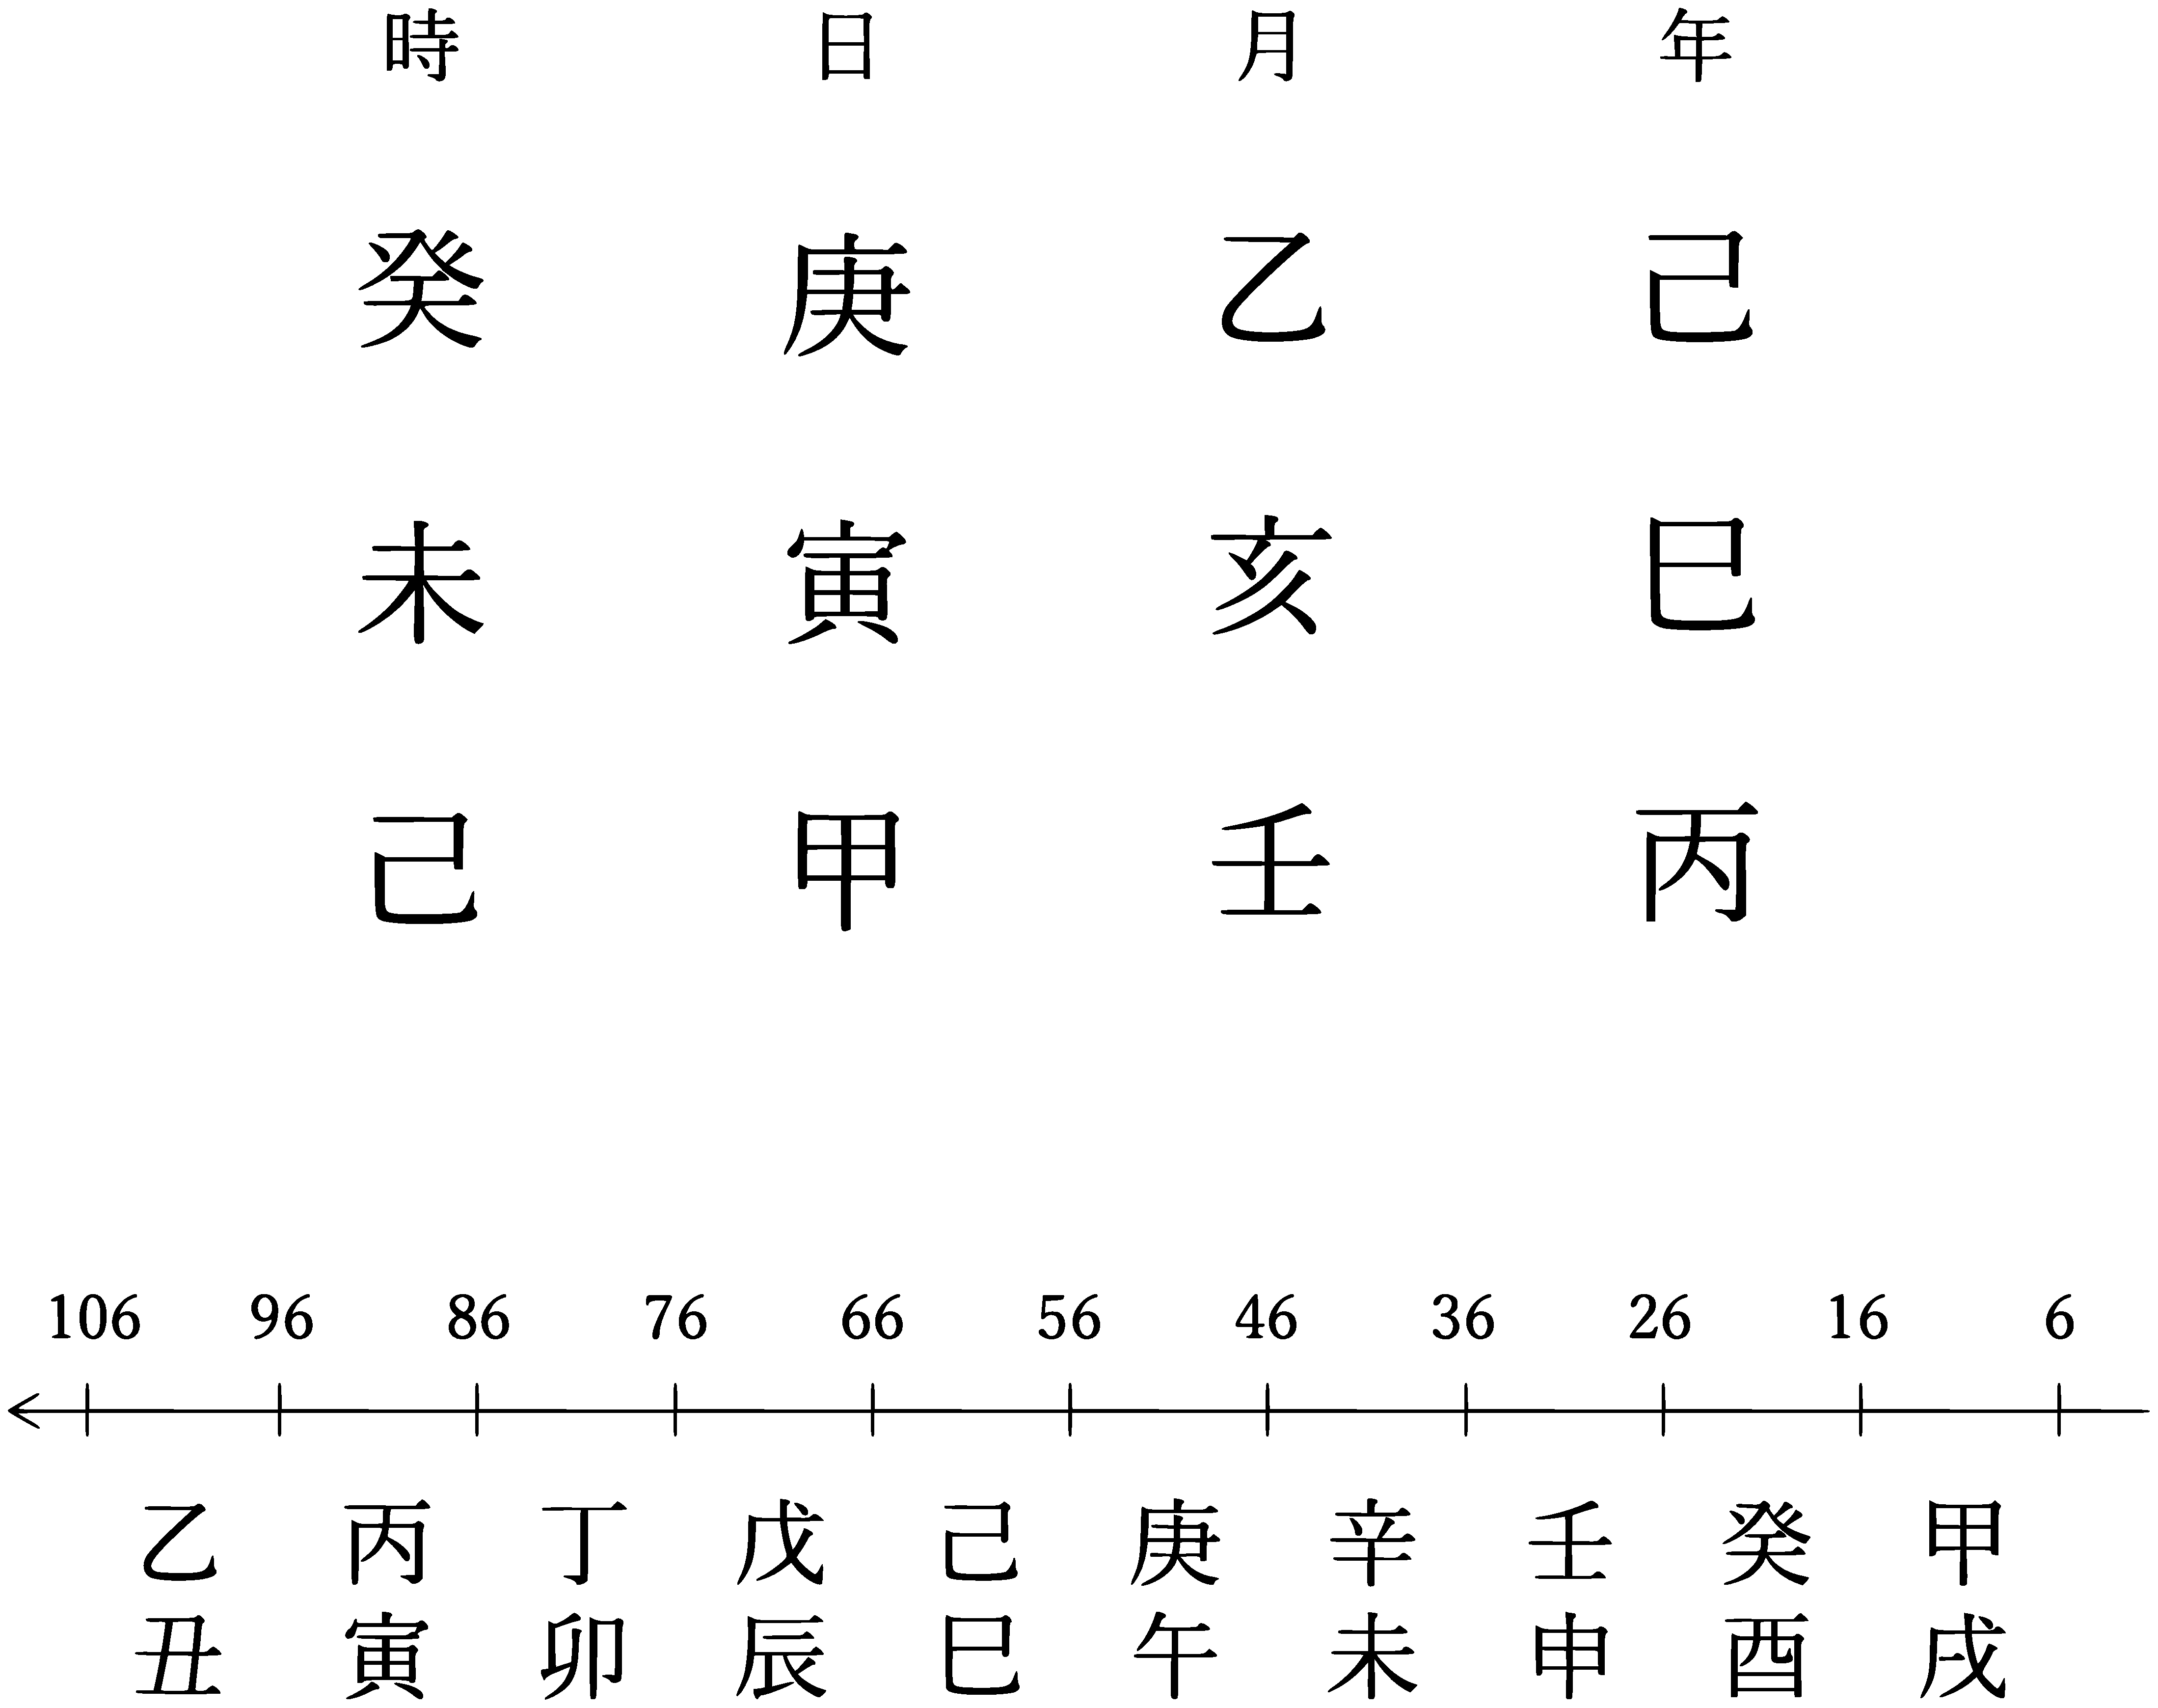
\includegraphics[width=72mm,angle=90]{figs/figure1-1.eps}
\end{wrapfigure}

命式は干支で表され、これがその人の持って生まれた先天運命を表します。命式を求める方法は機械的です。四柱推命学を志す人は、まずこれを求める方法に習熟する必要があります。

大運にもさまざまな要素が含まれ、これがその人の後天運勢を表します。命式と同様に、大運を求める方法も機械的です。やはりこれを求める方法にも習熟する必要があります。

命式・大運を求めた後、これらを詳細に解釈することによって、その人の運命・運勢を推測します。これにより、その人の性質、適職指向、人事・事相、肉親関係など、多岐にわたる事柄を明らかにできます。

例えば、先の男性は、才智に富み活動家と命式から推測できます。また、社交的で人間関係も良好ですが、積極性に欠けるところに注意が必要となるでしょう。さらに、\rensuji{45}歳までは良い運気が続きますが、それ以降は注意が必要となるため、若い時にできるだけ努力して将来に備えるべきことが、大運から推測できます。

このように、四柱推命学は、人間が生まれた年・月・日・時に基づいて、その先天運命と後天運勢とを推測する方法論です。各自の生まれながらに持っている質を知り、運気の流れを知り、人生航路で起きるさまざまな出来事や受難に対処する方法を考えるものです。

命式は、生年・月・日・時から一意に求められ、これは「持って生まれた運命」として換えようがありませんが、各人の人生が生まれながらに決定されているわけでは当然ありません。先天の運命が大輪の種子であったとしても、努力の時期を逸すれば花は咲きませんし、小さな草花の種子であったとしても、条件が整えば立派な花を咲かすことができます。四柱推命によって自分をよく知り、生涯の大局を見据えて、各自に応じた努力を積み重ねることにより、その後の運勢は必ず開かれるでしょう。


\subsection{五術体系における位置付け}

中国には、古来より「五術体系」と呼ばれる分類があります。\ruby{命}{めい}・\ruby{卜}{ぼく}・\ruby{相}{そう}・\ruby{医}{い}・\ruby{山}{ざん}の分類があり、これらはそれぞれ次の意味を持ちます。
\begin{description}
\item[\ruby{命}{めい}]命術のことで、生年・月・日・時に基づいて、先天運命と後天運勢とを推測する方法を指します。四柱推命はこの「命」に分類されます。その他、\ruby{紫微斗数}{しびとすう}、\ruby{九星気学}{きゅうせいきがく}などがこれにあたります。
\item[\ruby{卜}{ぼく}]卜術(\ruby{占卜}{せんぼく})のことで、偶然にあらわれた象徴を用いて、事柄や事態の成り行きを占う方法を指します。\ruby{周易}{しゅうえき}・\ruby{断易}{だんえき}・\ruby{梅花心易}{ばいかしんえき}などがこれにあたります。タロット・ルーンなども占卜に該当するでしょう。
\item[\ruby{相}{そう}]相術のことで、対象の姿・形から、その対象の状態や運勢を占う方法を指します。主なものとして、手相・人相・姓名判断・風水などがこれにあたります。
\item[\ruby{医}{い}]中国医術のことで、鍼灸・漢方・整体術などがこれにあたります。
\item[\ruby{山}{ざん}]大地自然の気をもらうことによって習得する術の総称で、気功・呼吸法・食事療法などがこれにあたります。
\end{description}

巷ではよく混同されていますが、四柱推命学は「占卜(占い)」ではありません。前述したとおり、「理屈」を積み上げて運命・運勢を推測する「命」であって、占卜のように「偶然」に頼る「卜」とは異なります。\footnote{そのため、サイコロやカードなどの小道具は一切用いません。}

そのため、「この時期にはこんなことが起こる」「この日は注意しなければ悪いことが起こる」「この時期に亡くなる」など、将来に起きる出来事を予言できるわけではありません。四柱推命学は、\ruby{看命}{かんめい}できる範囲は明確に決まっており、これを逸脱して不確かな推測を振り回すことを嫌います。\footnote{四柱推命学は「占い」ではないことから、対象を\ruby{看}{み}ることを「占う」とは言いません。「看命する」「鑑定する」などと言います。}

四柱推命学を真に志すのであれば、占卜との違いを理解した上で、理論・理屈から外れたことを云々することは控える自戒が必要です。

\subsection{概要のまとめ}
四柱推命学は「人間を知る学問」です。生年・月・日・時だけから、「命式」という航海図を描き、「大運」という天気予報を得る\ruby{命学}{めいがく}です。

こんな格言があります。\\

人事を尽くして天命を待つは常人なり

天命を知って人事を尽くすは達人なり\\

四柱推命学によって、各人が生まれながらに持っている天命(質)をよく知り、自分の生涯のうち、いつ花が咲くか、いつ注意すればよいかを予測します。そして、発展運の時は大いに伸ばし、凶運の時は大難を小難に止める人事を尽くせば、人生の「達人」といえるかもしれません。

それでは、奥深い四柱推命学の世界に足を踏み入れましょう。本書がその正しい第一歩となることを願っています。

\clearpage

\section{予備知識}

この章では、四柱推命学を学び進めるために必要となる最も基本的なことを解説します。普段は馴染みのない用語が多数出てきますが、少しずつ慣れていきましょう。

\subsection{陰陽五行と干支}
\subsubsection*{陰陽五行説}
陰陽説は、世界が陰と陽のバランスから成り立っていると考える思想です。例えば、「太陽と月」「天と地」「昼と夜」「男と女」「裏と表」など、自然界の全てのものを「陰」と「陽」の相反する二つの要素でとらえます。そして、これらが互いに消長し、調和することによって自然界の秩序が保たれていると解釈します。

一方で、五行説は、万物が\ruby{木}{もく}・\ruby{火}{か}・\ruby{土}{ど}・\ruby{金}{ごん}・\ruby{水}{すい}の五つの要素(五行)から構成されていると考える思想です。そして、これらの要素の盛衰・消長によって、この世のすべてが循環して進展すると解釈します。

そして「陰陽五行説」は、陰陽説と五行説とが結びついた古代中国の思想です。四柱推命学では、この陰陽五行説に基づいて、\textbf{陰陽・五行の均衡・不均衡を検討すること}が、最大のポイントとなります。

\subsubsection*{\ruby{十干}{じっかん}}

陰陽説によれば、すべてのものに陰陽がありますので、\ruby{木}{もく}・\ruby{火}{か}・\ruby{土}{ど}・\ruby{金}{ごん}・\ruby{水}{すい}の五行にもそれぞれ陰陽があることになります。

ここで、中国の慣習にしたがって陽を「\ruby{兄}{え}」に、陰を「\ruby{弟}{と}」に対応づけ、これらの陰陽五行の十種類を漢字で表現すると、次の表のようになります。

\begin{figure}[hbp]
  \centering
  
\includegraphics[width=50mm,angle=90]{figs/table2-1.eps}
\end{figure}

例えば、「\ruby{木}{もく}」の五行の陽は「\ruby{木}{き}の\ruby{兄}{え}」となり、「\ruby{甲}{きのえ}」の漢字で表現します。また、「\ruby{金}{ごん}」の五行の陰は「\ruby{金}{か}の\ruby{弟}{と}」となり、「\ruby{辛}{かのと}」の漢字で表現します。\footnote{「金」が変則的な読み方(ごん、か)になることに注意しましょう。}

このように、陰陽五行の十種類を漢字で表現したものを「\ruby{十干}{じっかん}」と呼びます。

また、\ruby{甲}{きのえ}・\ruby{丙}{ひのえ}・\ruby{戊}{つちのえ}・\ruby{庚}{かのえ}・\ruby{壬}{みずのえ}(\ruby{兄}{え}のグループ)を「\ruby{陽干}{ようかん}」と呼び、\ruby{乙}{きのと}・\ruby{丁}{ひのと}・\ruby{己}{つちのと}・\ruby{辛}{かのと}・\ruby{癸}{みずのと}(\ruby{弟}{と}のグループ)を「\ruby{陰干}{いんかん}」と呼びます。

四柱推命学では、この十干が一つの基礎になりますので、まずは漢字の表記と読みを正しく覚えておく必要があります。

\subsubsection*{\ruby{十二支}{じゅうにし}}

\ruby{十二支}{じゅうにし}は、\ruby{子}{ね}、\ruby{丑}{うし}、\ruby{寅}{とら}、\ruby{卯}{う}、\ruby{辰}{たつ}、\ruby{巳}{み}、\ruby{午}{うま}、\ruby{未}{ひつじ}、\ruby{申}{さる}、\ruby{酉}{とり}、\ruby{戌}{いぬ}、\ruby{亥}{い}の総称です。日本では年を表す\ruby{干支}{えと}として馴染み深いものです。

十二支にも陰陽・五行の分類があり、それぞれ次の表のようになります。

また、\ruby{子}{ね}・\ruby{寅}{とら}・\ruby{辰}{たつ}・\ruby{午}{うま}・\ruby{申}{さる}・\ruby{戌}{いぬ}を「\ruby{陽支}{ようし}」と呼び、\ruby{丑}{うし}・\ruby{卯}{う}・\ruby{巳}{み}・\ruby{未}{ひつじ}・\ruby{酉}{とり}・\ruby{亥}{い}を「\ruby{陰支}{いんし}」と呼びます。

四柱推命学では、命式・大運をすべて\ruby{十干}{じっかん}と\ruby{十二支}{じゅうにし}で表しますので、\ruby{十干}{じっかん}だけでなく、\ruby{十二支}{じゅうにし}の表記と読みも覚えておく必要があります。

\begin{figure}[h]
  \centering
  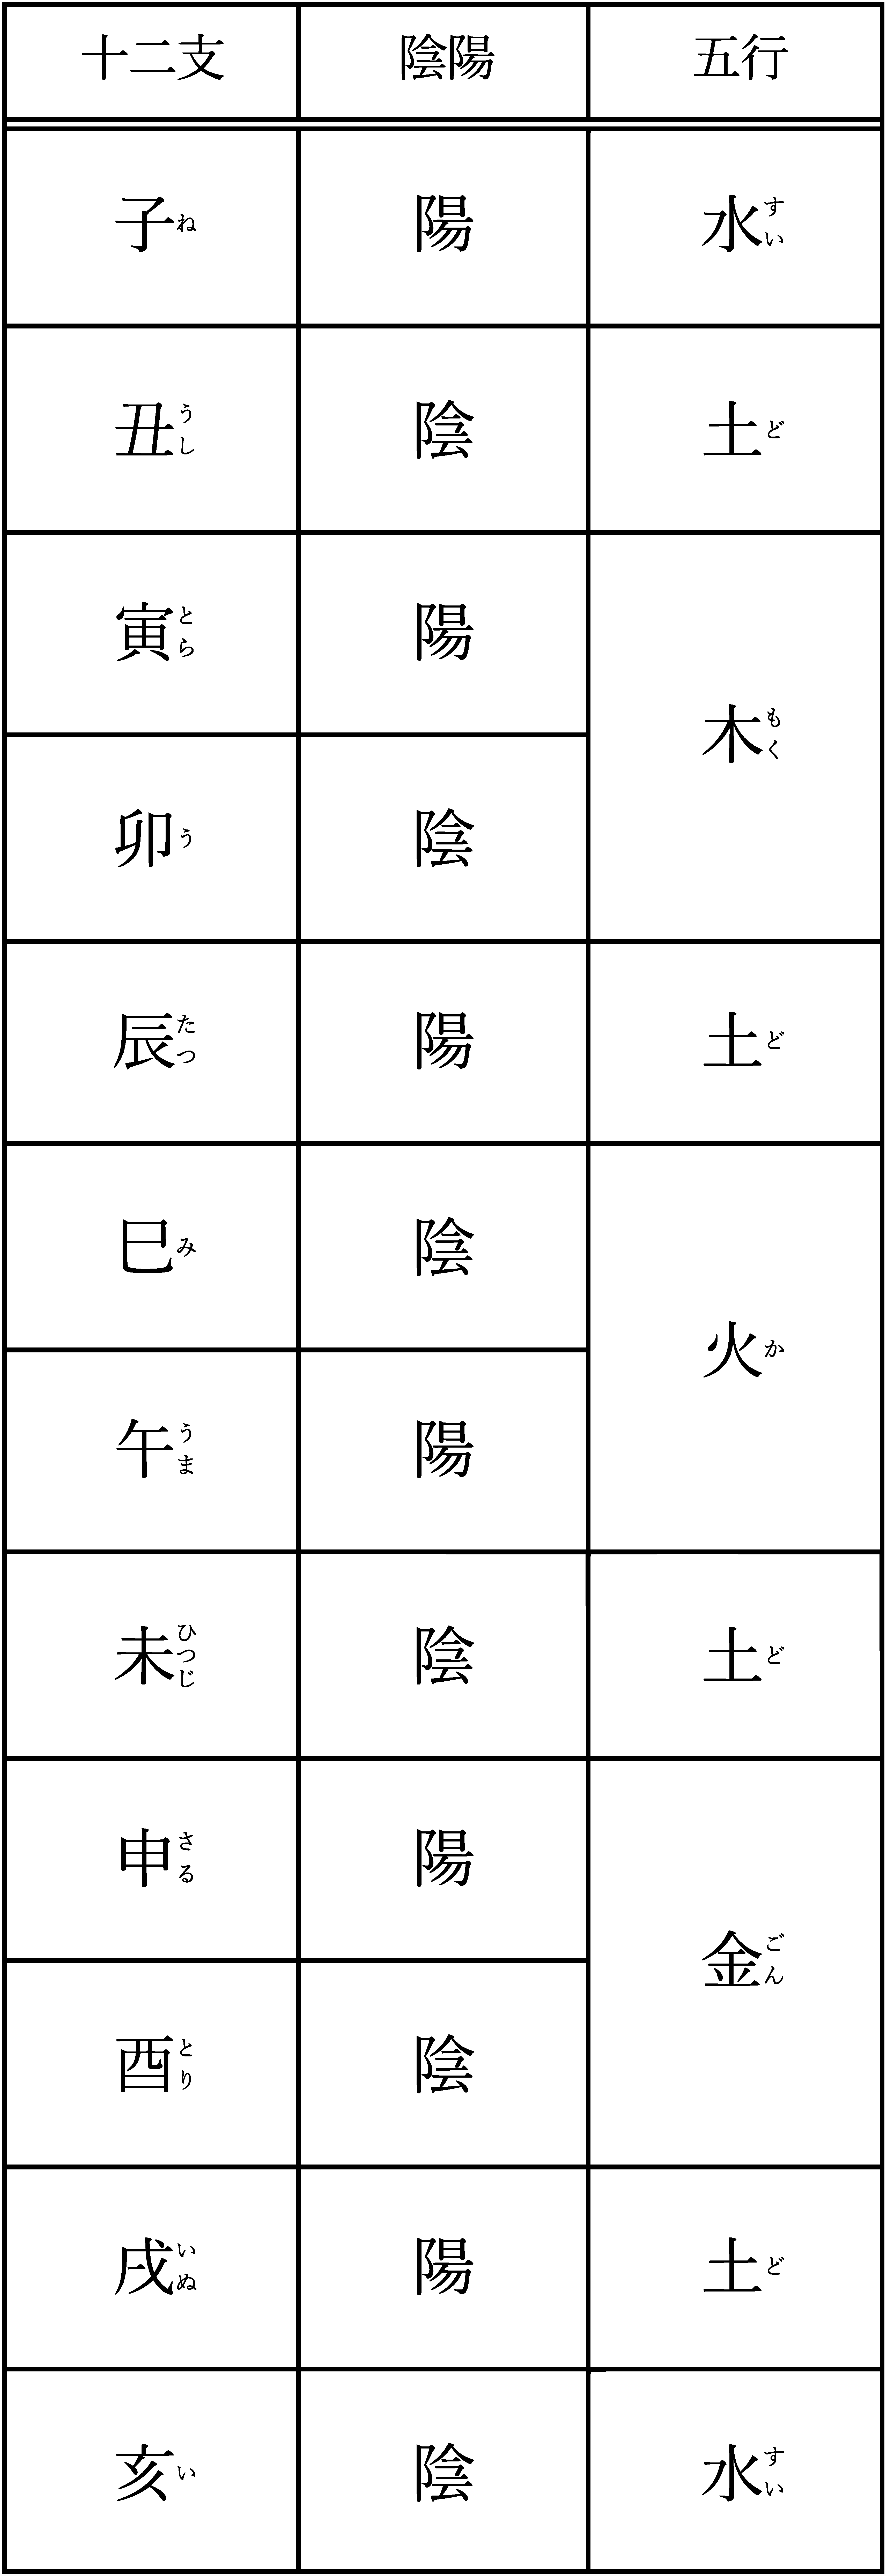
\includegraphics[width=48mm,angle=90]{figs/table2-2.eps}
\end{figure}


\subsubsection*{\ruby{干支}{かんし}}

\ruby{十干}{じっかん}と\ruby{十二支}{じゅうにし}を合わせた十干十二支を「\ruby{干支}{かんし}」と略して呼びます。\ruby{干支}{えと}と漢字が同じですが、意味も読み方も異なりますので注意しましょう。\footnote{以後「干支」はすべて「かんし」と読みます。}

陽干と陽支、陰干と陰支を任意に組み合わせると、六〇通りの干支を構成できます。これを表にしたものを「\ruby{六十干支}{ろくじっかんし}表」と呼びます。\footnote{表の最下段に記載の「\ruby{空亡}{くうぼう}」については、後の章で詳しく説明します。}

\begin{figure}[h]
  \centering
  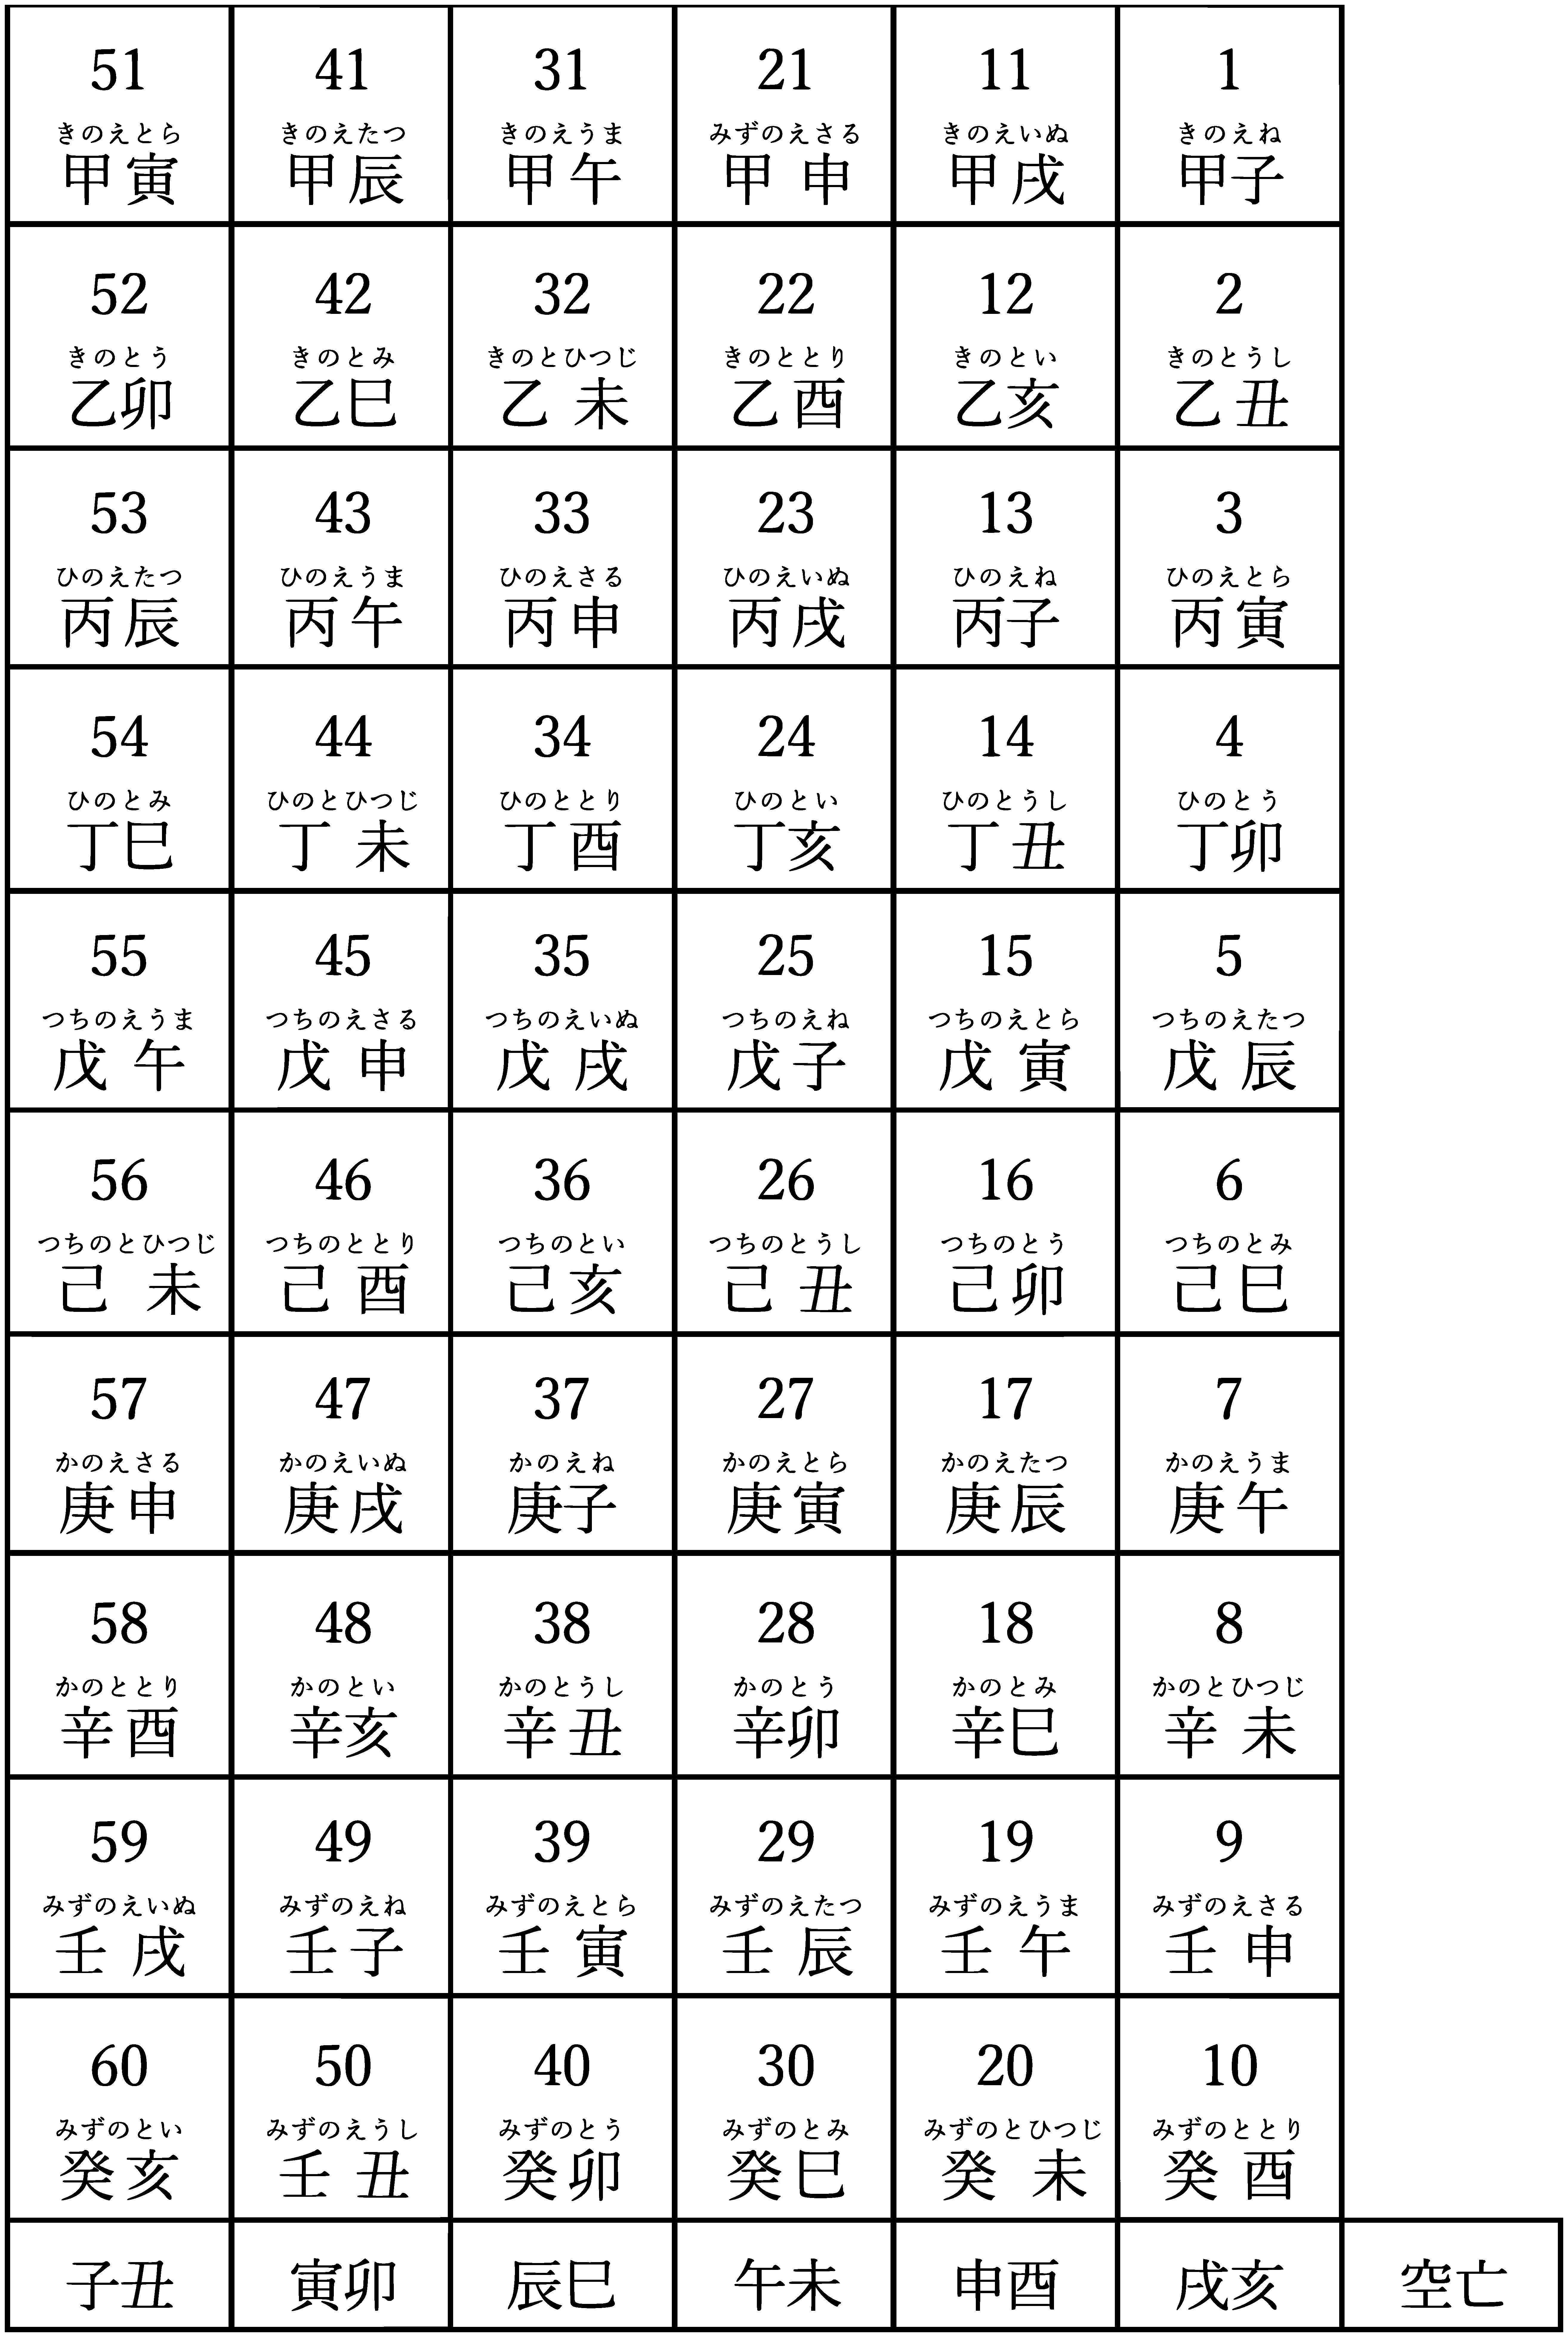
\includegraphics[width=75mm,angle=90]{figs/table2-3.eps}
\end{figure}

中国では、古代からこの六十干支を用いて暦を記録していました。私たちが普段使う近代西洋の「\ruby{天文暦}{てんもんれき}」に対して、これを「\ruby{干支暦}{かんしれき}」と呼びます。

六十干支は、表のように「\ruby{甲子}{きのえね}」(1)から始まり「\ruby{癸亥}{みずのとい}」(\rensuji{60})で終わります。一巡すると、また「\ruby{甲子}{きのえね}」から始まり、この六十干支表の番号順に、年・月・日・時の干支が延々と巡ります。

例えば、最近では大正\rensuji{13}年(1924年)が「\ruby{甲子}{きのえね}」であり、それより六〇年後の昭和\rensuji{59}年(1984年)も「\ruby{甲子}{きのえね}」でした。同様に、2044年も「\ruby{甲子}{きのえね}」になります。余談ですが、甲子園球場は、大正\rensuji{13}年の「\ruby{甲子}{きのえね}」年に完成したことにちなんで、その名が付けられました。六〇歳を「還暦」と呼ぶのも、「暦が\ruby{還}{かえ}る」ことからきています。

また、令和3年(2022年)8月は「\ruby{己酉}{つちのととり}」であり、同月\rensuji{17}日は「\ruby{壬寅}{みずのえとら}」でした。そのため、六〇月後の令和8年(2027年)8月も「\ruby{己酉}{つちのととり}」であり、六〇日後の\rensuji{10}月\rensuji{16}日も「\ruby{壬寅}{みずのえとら}」でした。

さらに、令和元年(2019年)5月\rensuji{13}日\rensuji{13}時0分は「\ruby{癸未}{みずのとひつじ}」だったため、六〇時間後の同月\rensuji{18}日\rensuji{13}時0分も「\ruby{癸未}{みずのとひつじ}」でした。

このように、年・月・日・時の干支が、古代から六〇サイクルにより休みなく巡っています。

四柱推命学では、\textbf{天文暦で表される生年・月・日・時を、干支暦で表される生年・月・日・時に置き換えることが最初の一歩}となります。


\subsection{五行と季節の関係}

\ruby{木}{もく}・\ruby{火}{か}・\ruby{土}{ど}・\ruby{金}{ごん}・\ruby{水}{すい}の五行には、次の表のようにそれぞれ季節が対応づけられています。

\begin{figure}[h]
  \centering
  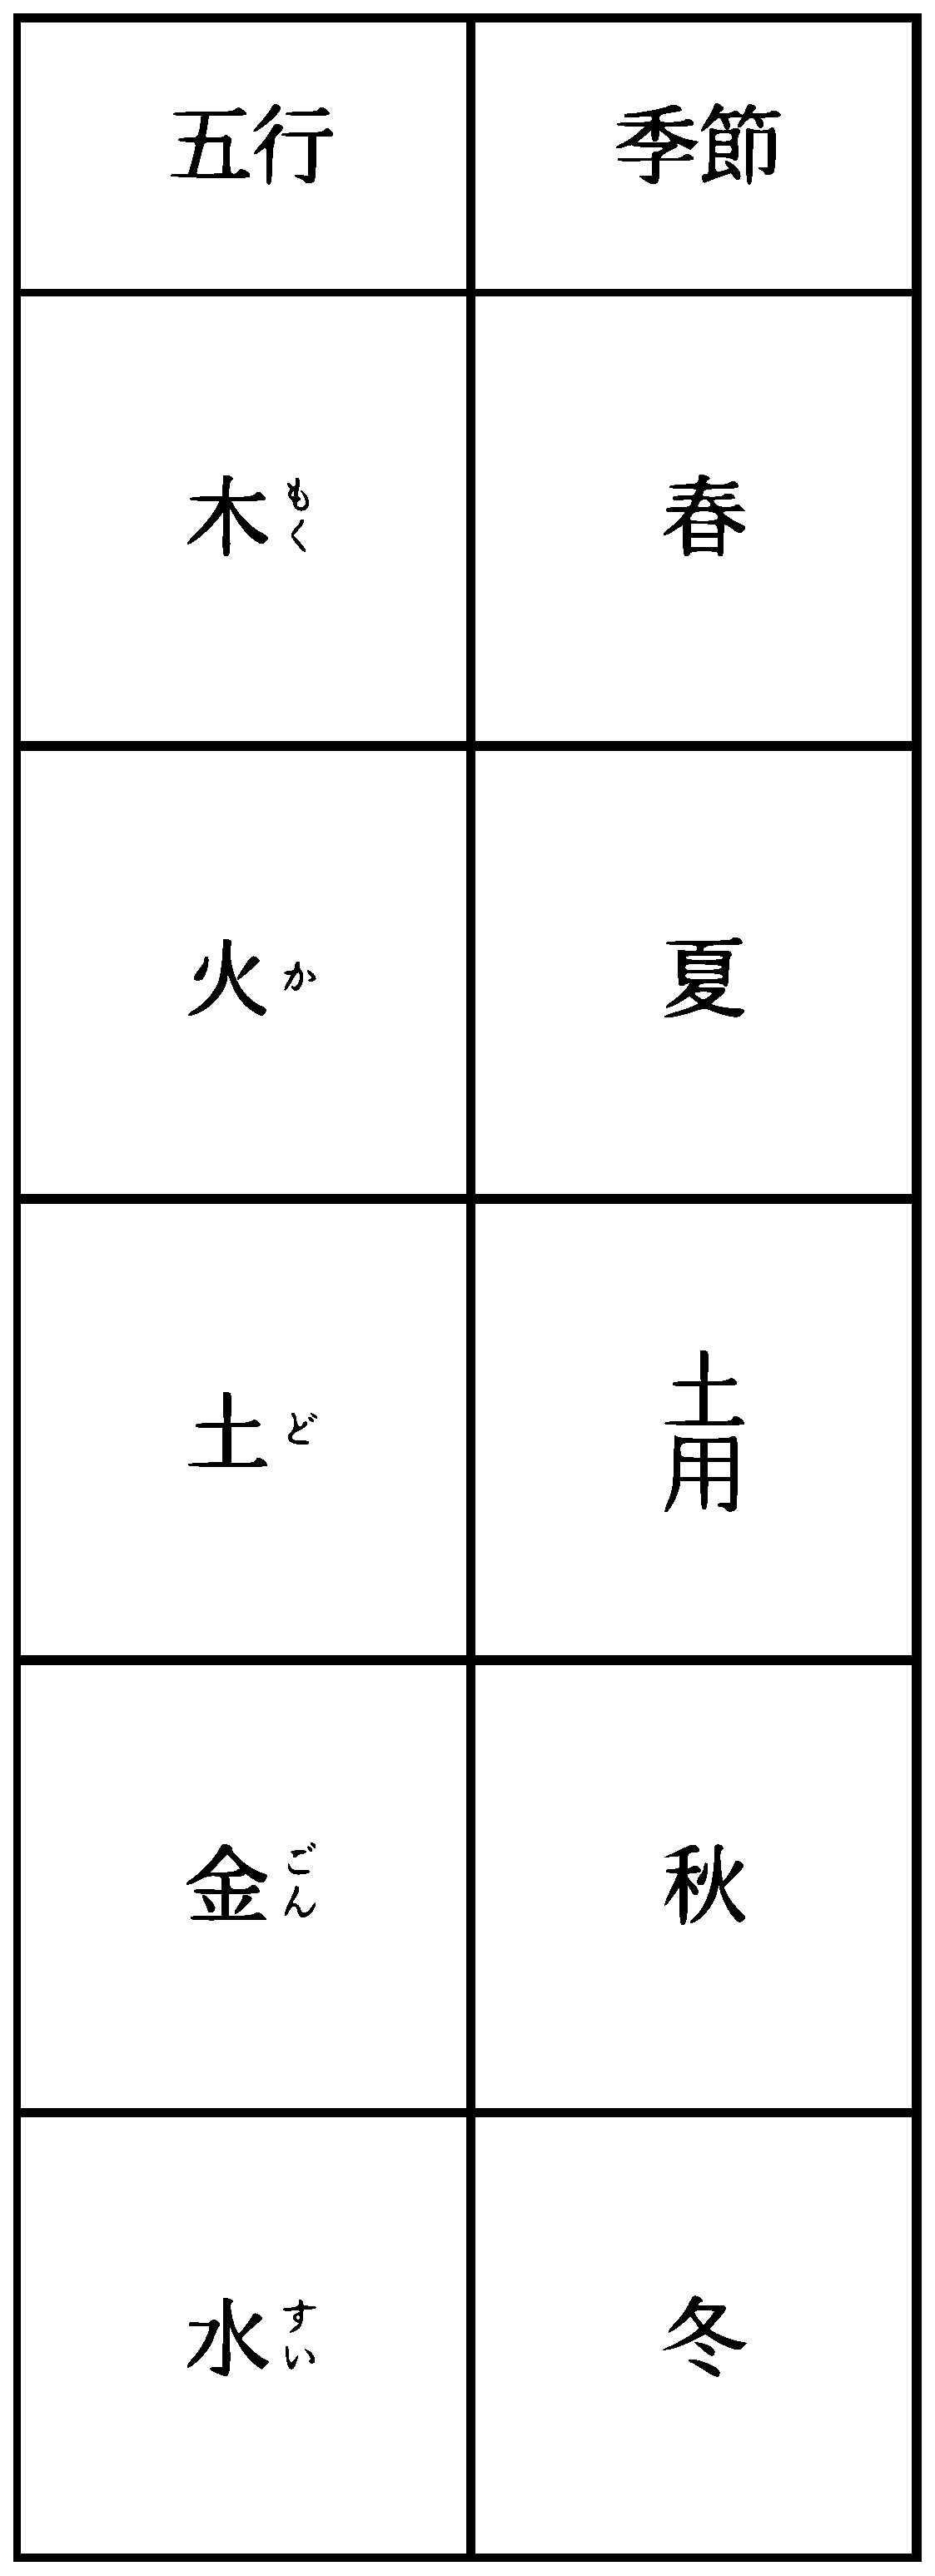
\includegraphics[width=30mm,angle=90]{figs/table2-4.eps}
\end{figure}

「木」が青葉となり茂る季節が春、「火」が燃えるように暑くなる季節が夏、「金」が土の中で実る季節が秋、「水」が冷たく凍る季節が冬に対応します。「土」は、それぞれの季節の終わりを表し、これを「土用」といいます。\footnote{いわゆる「土用の丑」は、暦の上での夏(七月)の土用(立秋まえの十八日間)をいいます。}

四柱推命学は季節を重視します。人間の運勢にも「季節」があり、その移ろいに応じて人生にさまざまな変化をもたらすと考えるからです。

例えば、大運に「春」が巡った場合、命式に含まれる木の五行(\ruby{甲}{きのえ}、\ruby{乙}{きのと})が\ruby{旺}{おう}じます。\footnote{「\ruby{旺}{おう}じる」とは、その五行の作用が大きくなることをいいます。}

同様に、「夏」が巡った場合は火の五行(\ruby{丙}{ひのえ}、\ruby{丁}{ひのと})が、「秋」が巡った場合は金の五行(\ruby{庚}{かのえ}、\ruby{辛}{かのと})が、「冬」が巡った場合は水の五行(\ruby{壬}{みずのえ}、\ruby{癸}{みずのと})が旺じます。そして、それぞれの季節の終わり(土用)には土の五行(\ruby{戊}{つちのえ}、\ruby{己}{つちのと})が旺じます。その結果、命式において他の五行との相対的な関係がダイナミックに変化し、これが運勢の吉凶を決定づけることになります。


\subsection{予備知識のまとめ}

四柱推命学の予備知識として、五行、十干、十二支、季節について説明しましたが、この内容をあらためて表にすると次のようになります。

\begin{figure}[hbp]
  \centering
  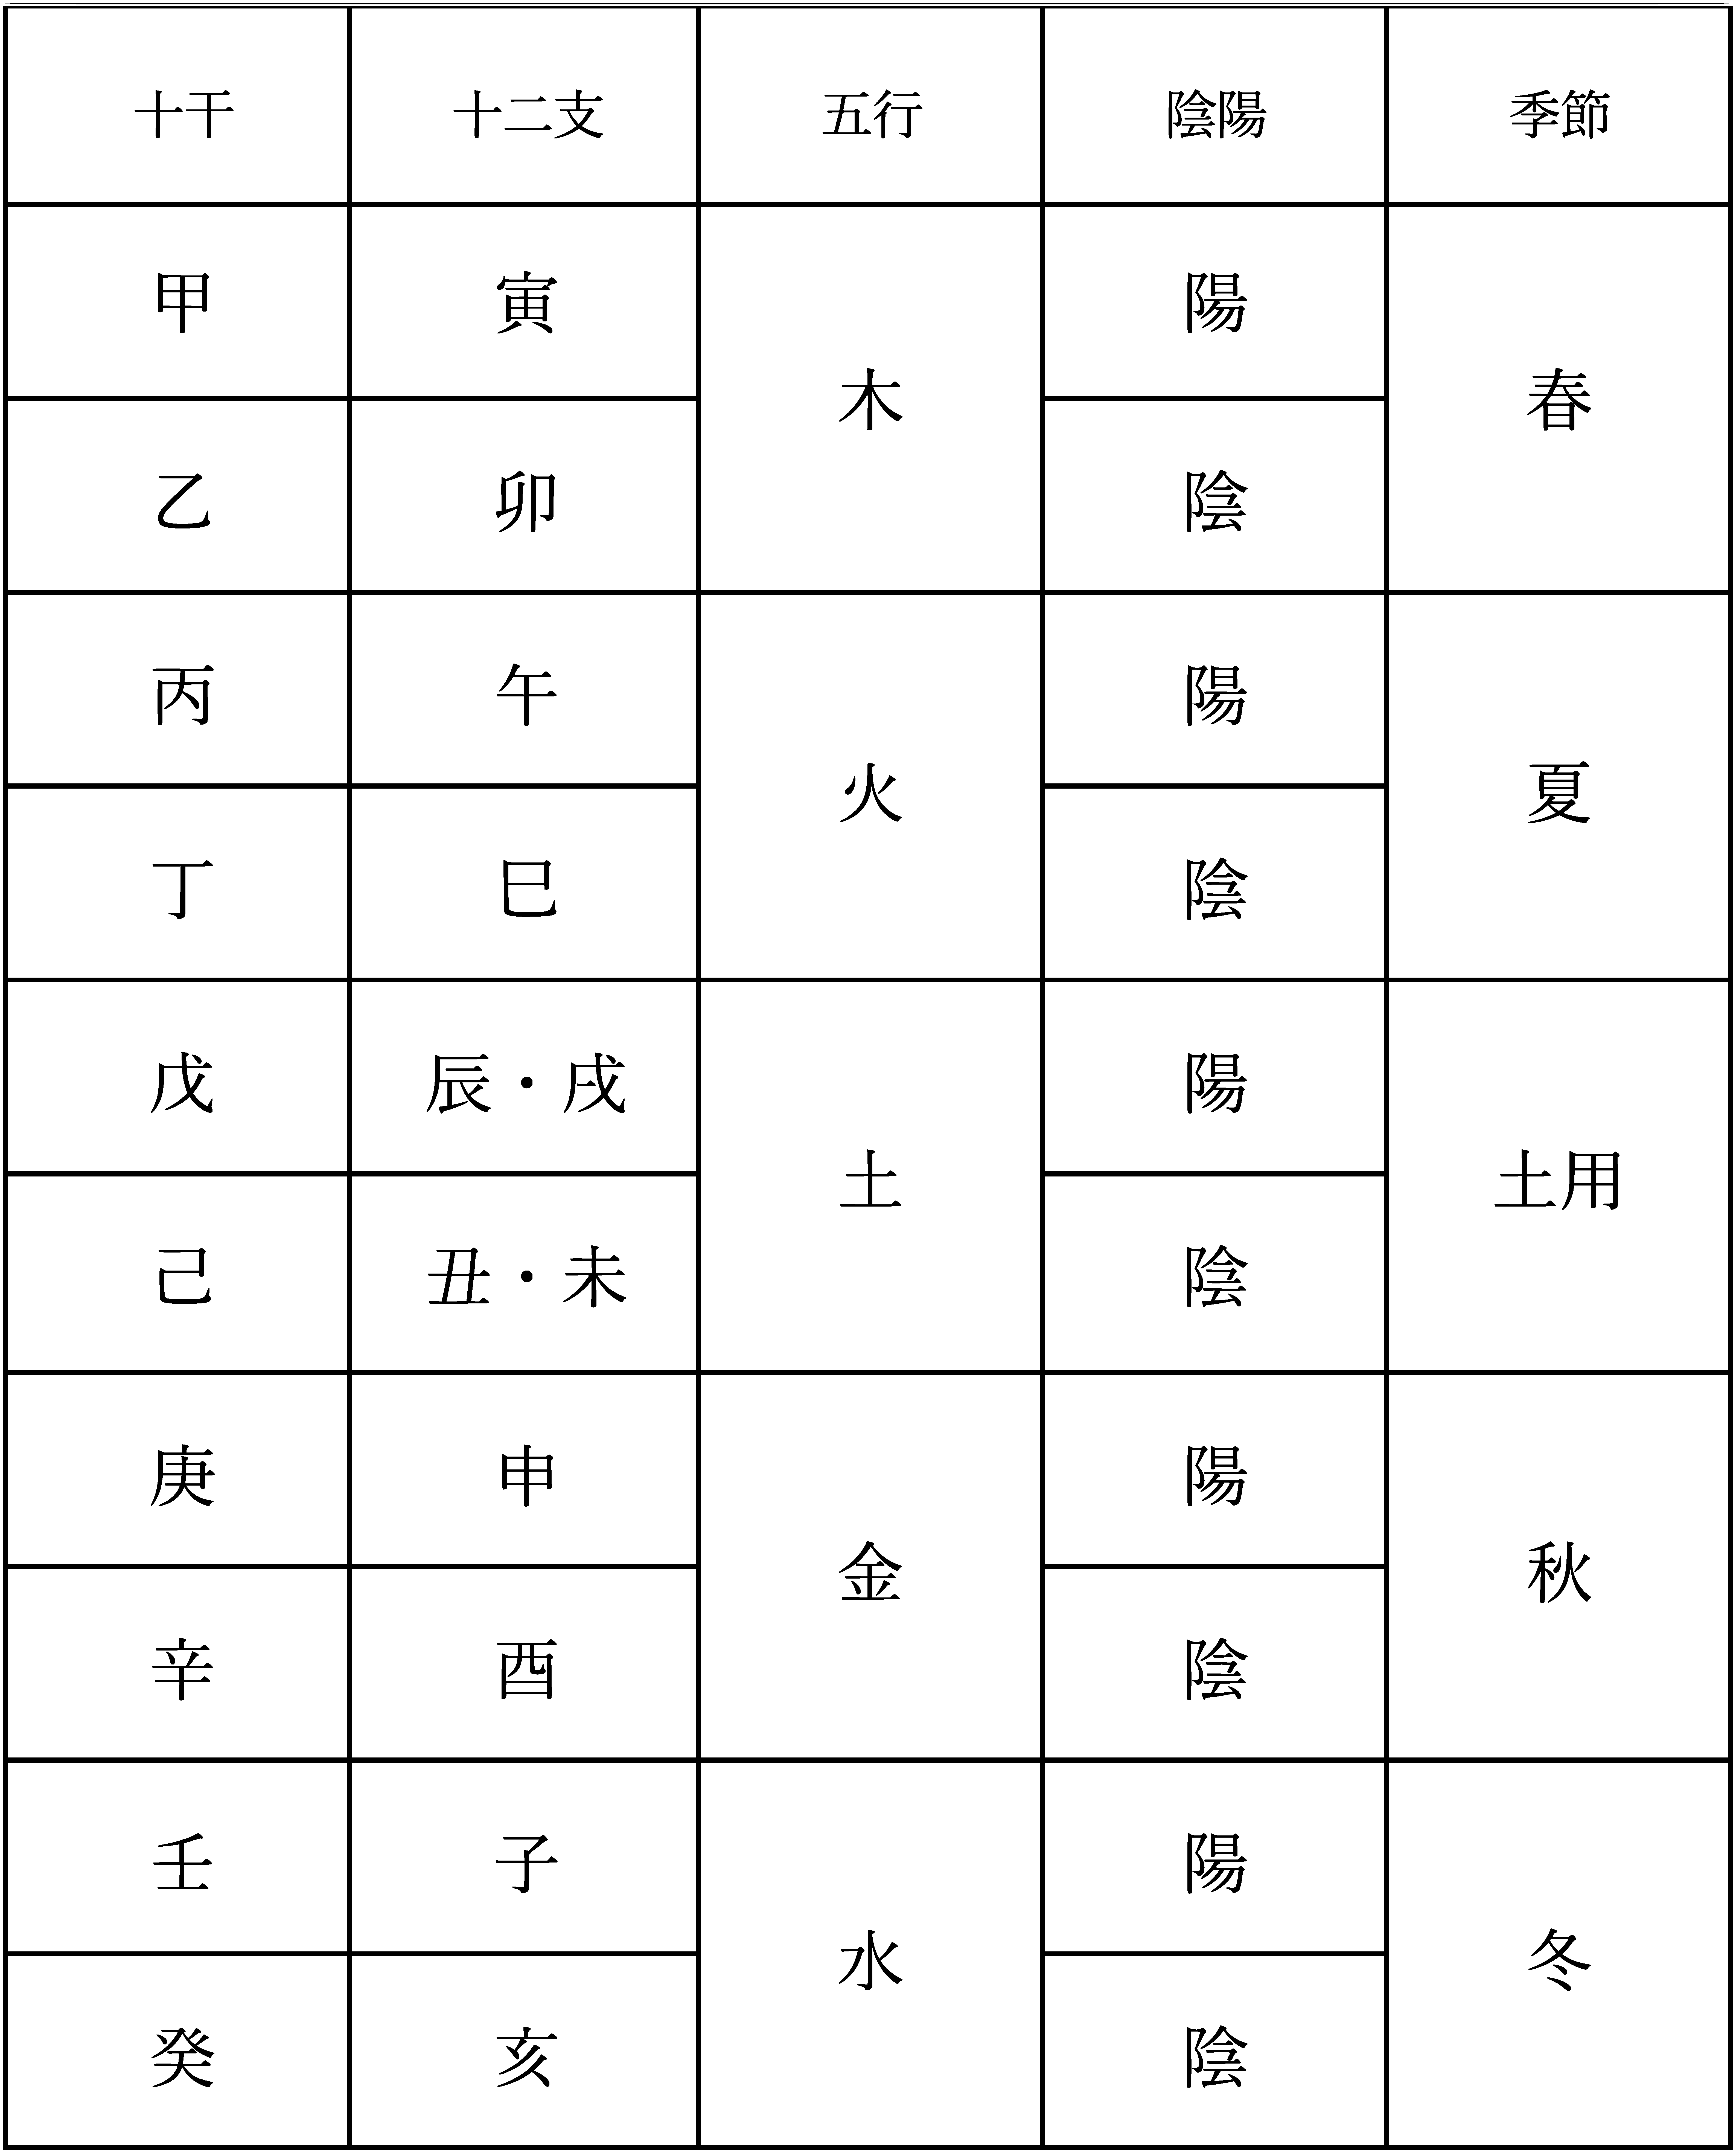
\includegraphics[width=82mm,angle=90]{figs/table2-5.eps}
\end{figure}

まとめると、まず五行(\ruby{木}{もく}・\ruby{火}{か}・\ruby{土}{ど}・\ruby{金}{ごん}・\ruby{水}{すい})があり、これらの陰陽によって\ruby{十干}{じっかん}(\ruby{甲}{きのえ}、\ruby{乙}{きのと}、\ruby{丙}{ひのえ}、\ruby{丁}{ひのと}、\ruby{戊}{つちのえ}、\ruby{己}{つちのと}、\ruby{庚}{かのえ}、\ruby{辛}{かのと}、\ruby{壬}{みずのえ}、\ruby{癸}{みずのと})が導かれます。そして、この十干と十二支(\ruby{子}{ね}、\ruby{丑}{うし}、\ruby{寅}{とら}、\ruby{卯}{う}、\ruby{辰}{たつ}、\ruby{巳}{み}、\ruby{午}{うま}、\ruby{未}{ひつじ}、\ruby{申}{さる}、\ruby{酉}{とり}、\ruby{戌}{いぬ}、\ruby{亥}{い})とを合わせて「\ruby{干支}{かんし}」と呼びます。人間の先天運命を表す命式も後天運勢を表す大運も、すべてこの干支で表現されます。

五行には季節が対応づけられています。\ruby{木}{もく}が春、\ruby{火}{か}が夏、\ruby{土}{ど}が土用、\ruby{金}{ごん}が秋、\ruby{水}{すい}が冬です。そして、十干では\ruby{甲}{きのえ}、\ruby{乙}{きのと}が、十二支では\ruby{寅}{とら}、\ruby{卯}{う}が「春」に対応します。同様に、\ruby{丙}{ひのえ}、\ruby{丁}{ひのと}、\ruby{巳}{み}、\ruby{午}{うま}が「夏」、\ruby{戊}{つちのえ}、\ruby{己}{つちのと}、\ruby{丑}{うし}、\ruby{辰}{たつ}、\ruby{未}{ひつじ}、\ruby{戌}{いぬ}が「土用」、\ruby{庚}{かのえ}、\ruby{辛}{かのと}、\ruby{申}{さる}、\ruby{酉}{とり}が「秋」、\ruby{壬}{みずのえ}、\ruby{癸}{みずのと}、\ruby{亥}{い}、\ruby{子}{ね}が「冬」に対応します。

このように、四柱推命学は陰陽五行説に立脚しており、これに基づいて陰陽・五行の均衡・不均衡を検討することがすべての基本となります。そのため、まずは五行・十干・十二支、およびこれらの季節との対応を、予備知識としてしっかり覚えておきましょう。


\clearpage

\section{命式}

\ruby{命式}{めいしき}は、生年・月・日・時を「\ruby{干支}{かんし}」に置き換え、「\ruby{年柱}{ねんちゅう}」「\ruby{月柱}{げっちゅう}」「\ruby{日柱}{にっちゅう}」「\ruby{時柱}{じちゅう}」として組み立てたものです。

\begin{wrapfigure}{l}[0pt]{0.25\textwidth}
  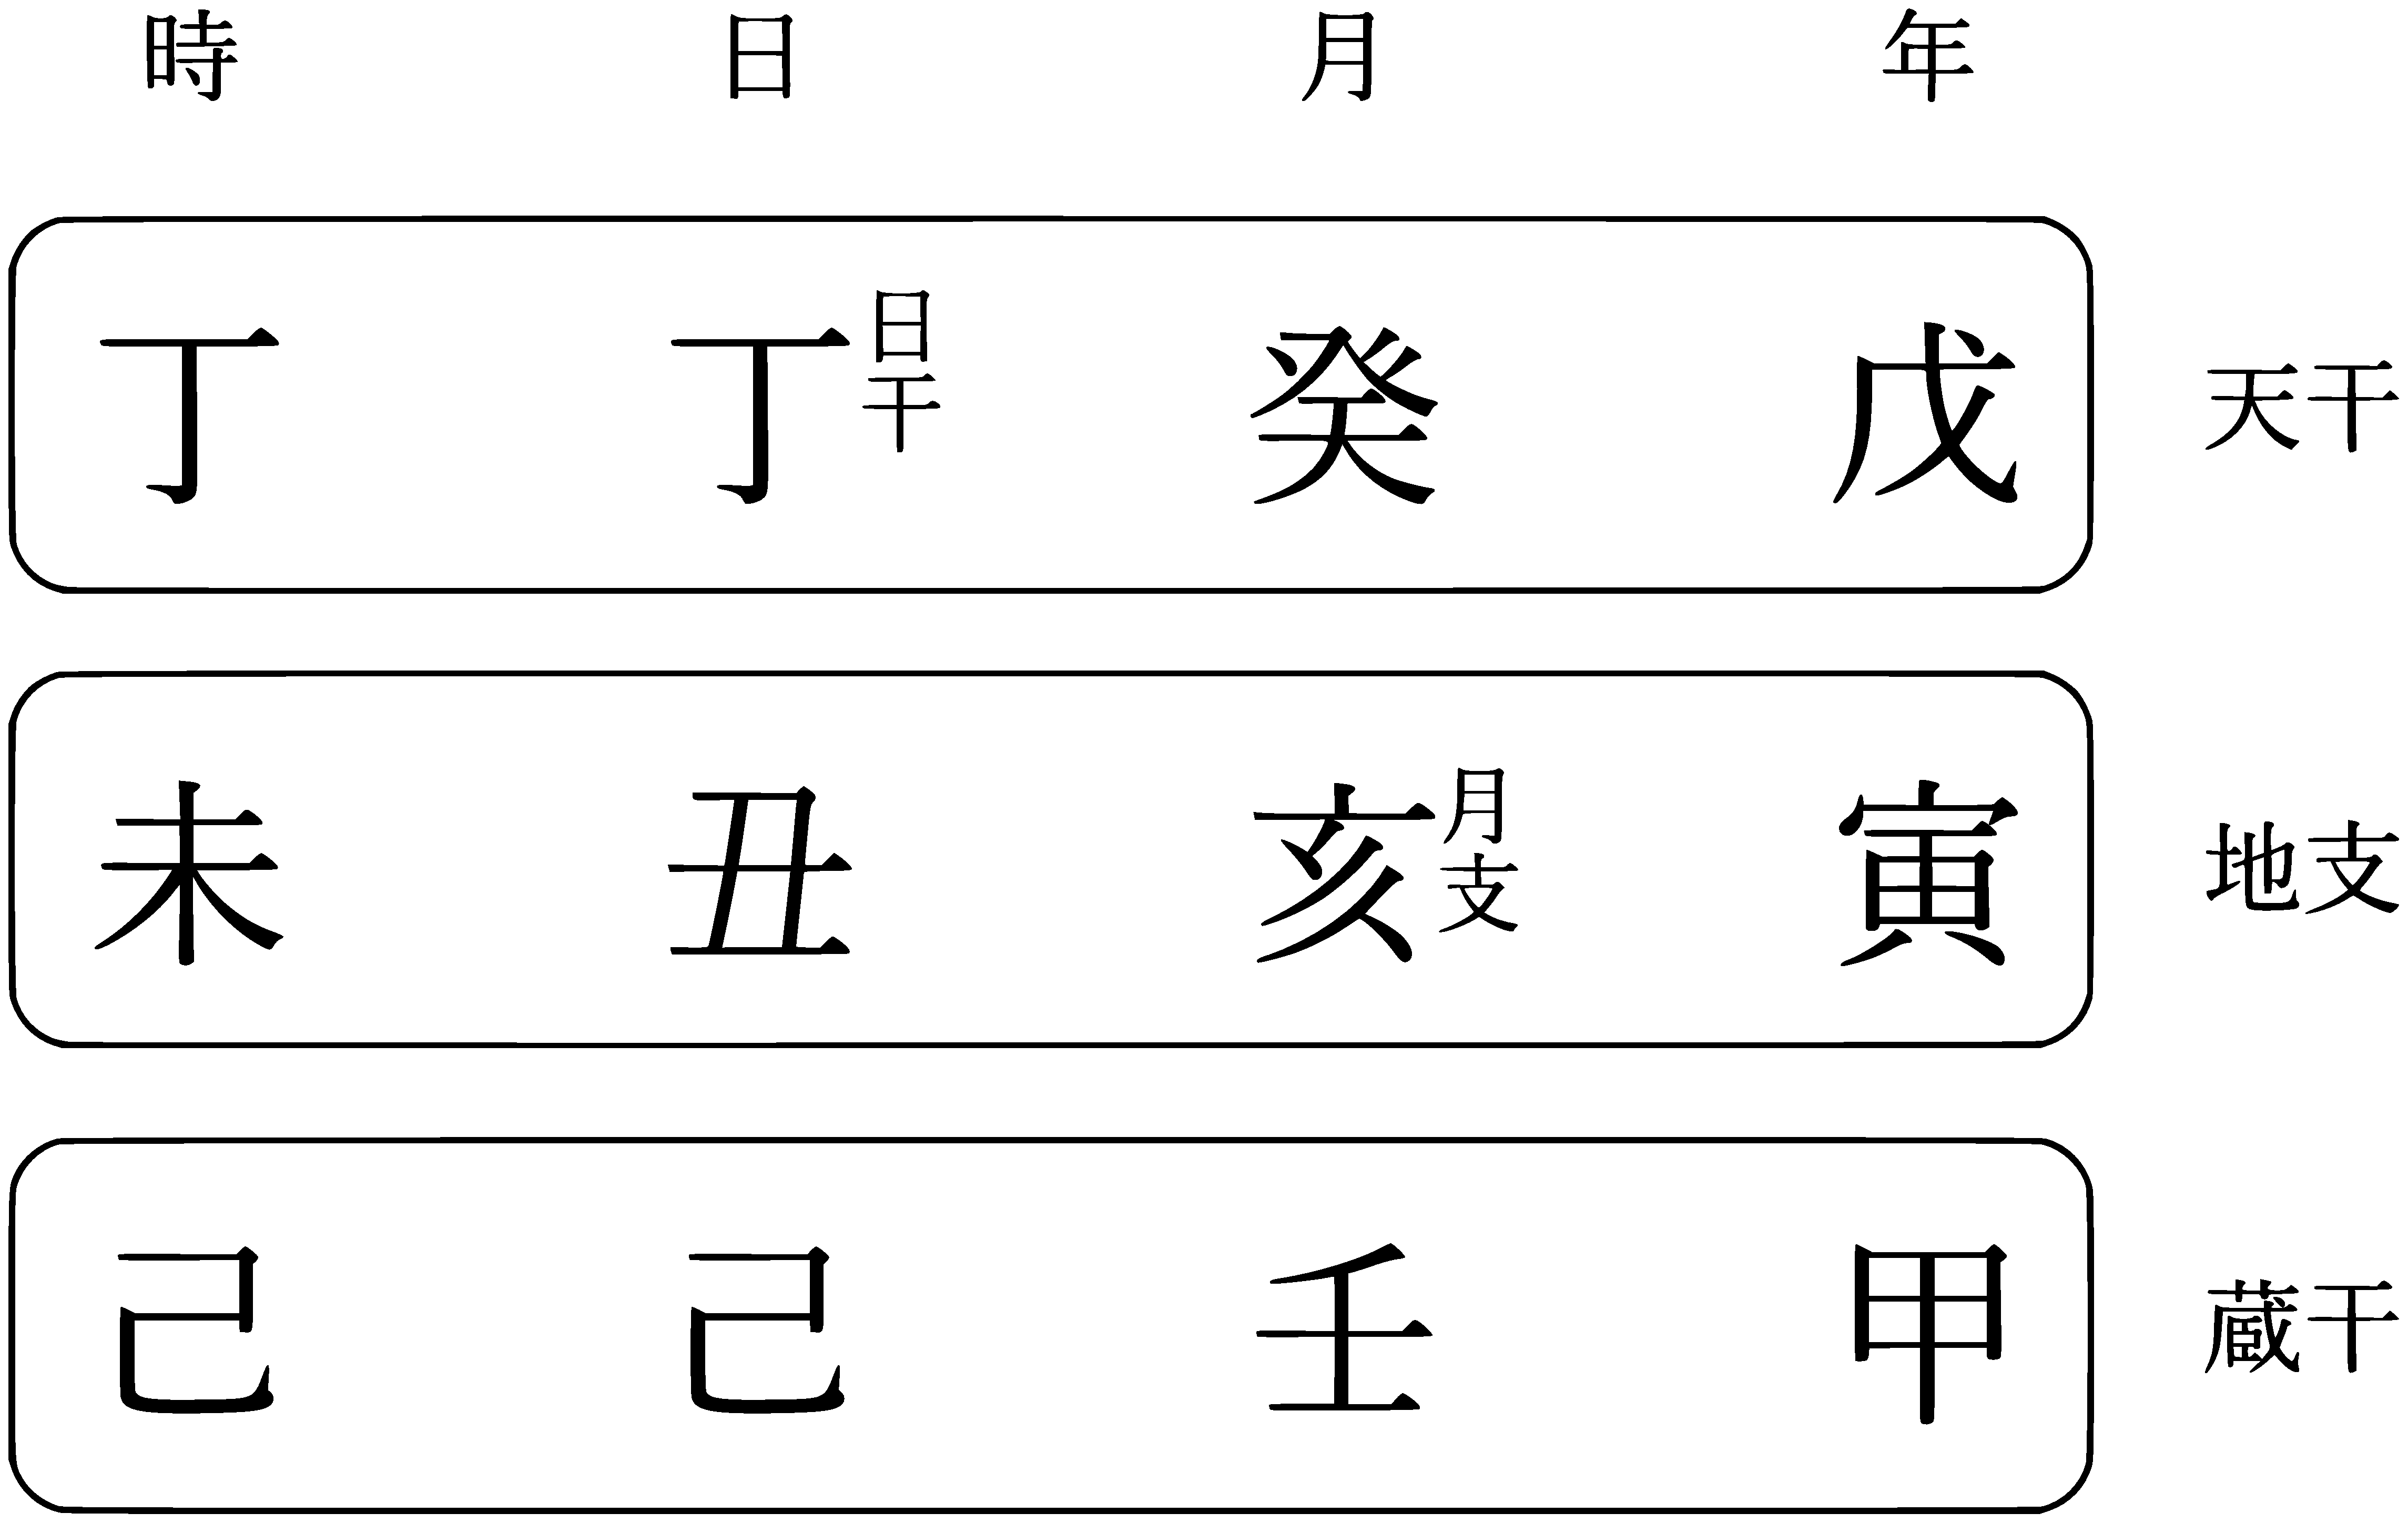
\includegraphics[width=60mm,angle=90]{figs/figure3-1.eps}
\end{wrapfigure}

男性の命式を「\ruby{男命}{だんめい}」、女性の命式を「\ruby{女命}{じょめい}」といい、主に先天運命を推測する(推命する)ために用います。このように、年・月・日・時に対応する干支を「四つの柱」として推命するため、「四柱推命」と称します。

命式において、上段の干を「\ruby{天干}{てんかん}」、中段の支を「\ruby{地支}{ちし}」、下段の干を「\ruby{蔵干}{ぞうかん}」と呼びます。特に重要な干支は、日柱に位置する天干と、月柱に位置する地支であり、これらをそれぞれ「\ruby{日干}{にっかん}」、「\ruby{月支}{げっし}」と略して呼びます。\footnote{月支ほど頻出ではありませんが、年柱地支を「年支」、日柱地支を「日支」、時柱地支を「時支」と呼ぶことがあります。また、日干のことを「\ruby{日元}{にちげん}」「\ruby{命主}{めいしゅ}」「\ruby{日主}{にっしゅ}」ということもあります。}

命式は、天文暦で表される生年・月・日・時を、干支暦で表される生年・月・日・時に置き換えることで四柱干支を求め、次に蔵干を導くという手順で構成するため、ここではこの順序で説明します。

\clearpage

\subsection{四柱干支の求め方}
\subsubsection*{年の干支の求め方}

和暦から年干支を得る手順は、次のとおりです。

\begin{enumerate}
\item 昭和であれば2を足し、平成であれば5を足し、令和であれば\rensuji{35}を足す(足した数が\rensuji{60}を超過している場合は\rensuji{60}を引く)
\item 足した数に対応する干支を六十干支表から得る\footnote{六十干支表は第二章参照。}
\end{enumerate}

例えば、平成\rensuji{10}年の場合、\rensuji{10}に5を足すと\rensuji{15}です。そこで、六十干支表の\rensuji{15}に対応する干支「戊寅」を得ます。

昭和\rensuji{59}年の場合、2を足すと\rensuji{61}となり、\rensuji{60}を超えてしまいます。この場合はさらに\rensuji{60}を引いて1とし、六十干支表の1に対応する干支「甲子」を得ます。

なお、西暦から年干支を求める手順は、次のとおりです。
\begin{enumerate}
\item 3を引く
\item 残りの数から直近の\rensuji{60}の倍数を引く
\item 引いた数に対応する干支を六十干支表から得る
\end{enumerate}

例えば、1998年の場合、まず3を引くと1995となり、ここから1980(直近の\rensuji{60}の倍数)を引くと\rensuji{15}です。そこで、六十干支表の\rensuji{15}に対応する干支「戊寅」を得ます。

\begin{wrapfigure}{l}[0pt]{0.2\textwidth}
  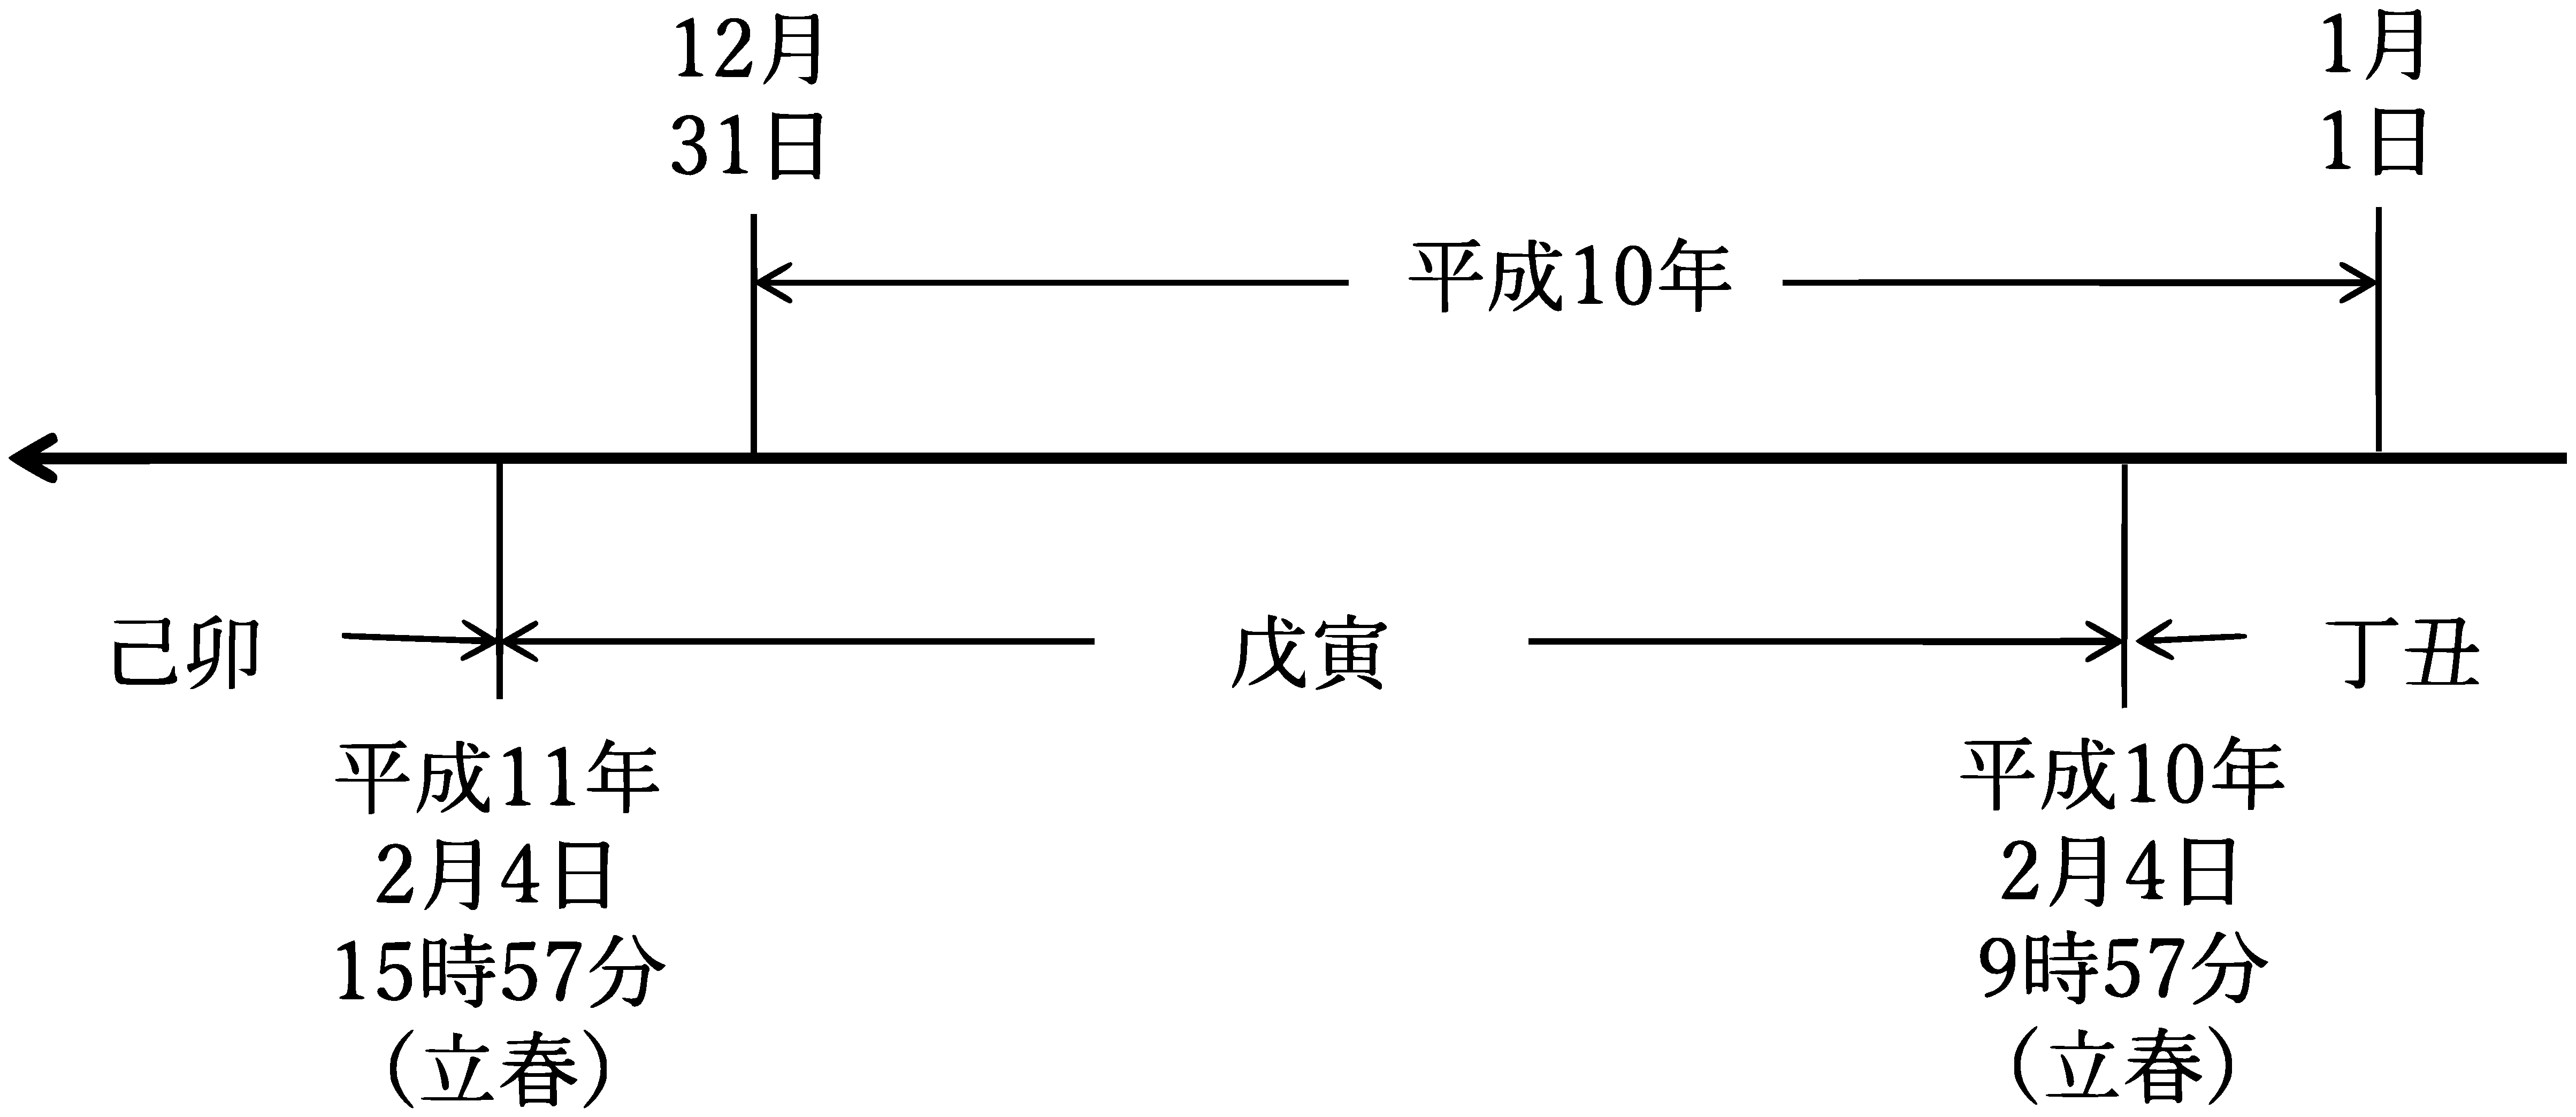
\includegraphics[width=65mm,angle=90]{figs/figure3-2.eps}
\end{wrapfigure}


年柱の干支を求める場合、注意しなければならないことがあります。それは、立春前までに誕生した人については、前年の干支を採用するということです。立春とは、暦の上で春に入る日であり、節分の翌日のことです。なお、暦の上での各月の始まりに入ることを「\ruby{節入}{せつい}りする」といいます。

この注意事項を、上の図を用いて説明します。

一般に、平成\rensuji{10}年は、その年の1月1日から\rensuji{12}月\rensuji{31}日までのことです。

一方で、四柱推命学では、平成\rensuji{10}年として「戊寅」の年柱を採用するのは、平成\rensuji{10}年2月4日9時\rensuji{57}分の節入りから、平成\rensuji{11}年2月4日\rensuji{15}時\rensuji{57}分の節入りより前までです。\footnote{立春の日付と正確な時刻については、国立天文台が発行する「理科年表」で毎年発表されています。}

例えば、平成\rensuji{10}年1月は、まだ「戊寅」には節入りしていませんので、その前年の「丁丑」を採用します。同様に、平成\rensuji{11}年2月1日も、まだ「己卯」に節入りしていませんので、その前年の「戊寅」を採用します。

このように、1月から2月の立春より前に生まれた人の年柱の求め方は変則的になるので、注意が必要です。


\subsubsection*{月の干支の求め方}

月の干支は、次の月干支表を用いて求めます。

\begin{figure}[h]
  \centering
  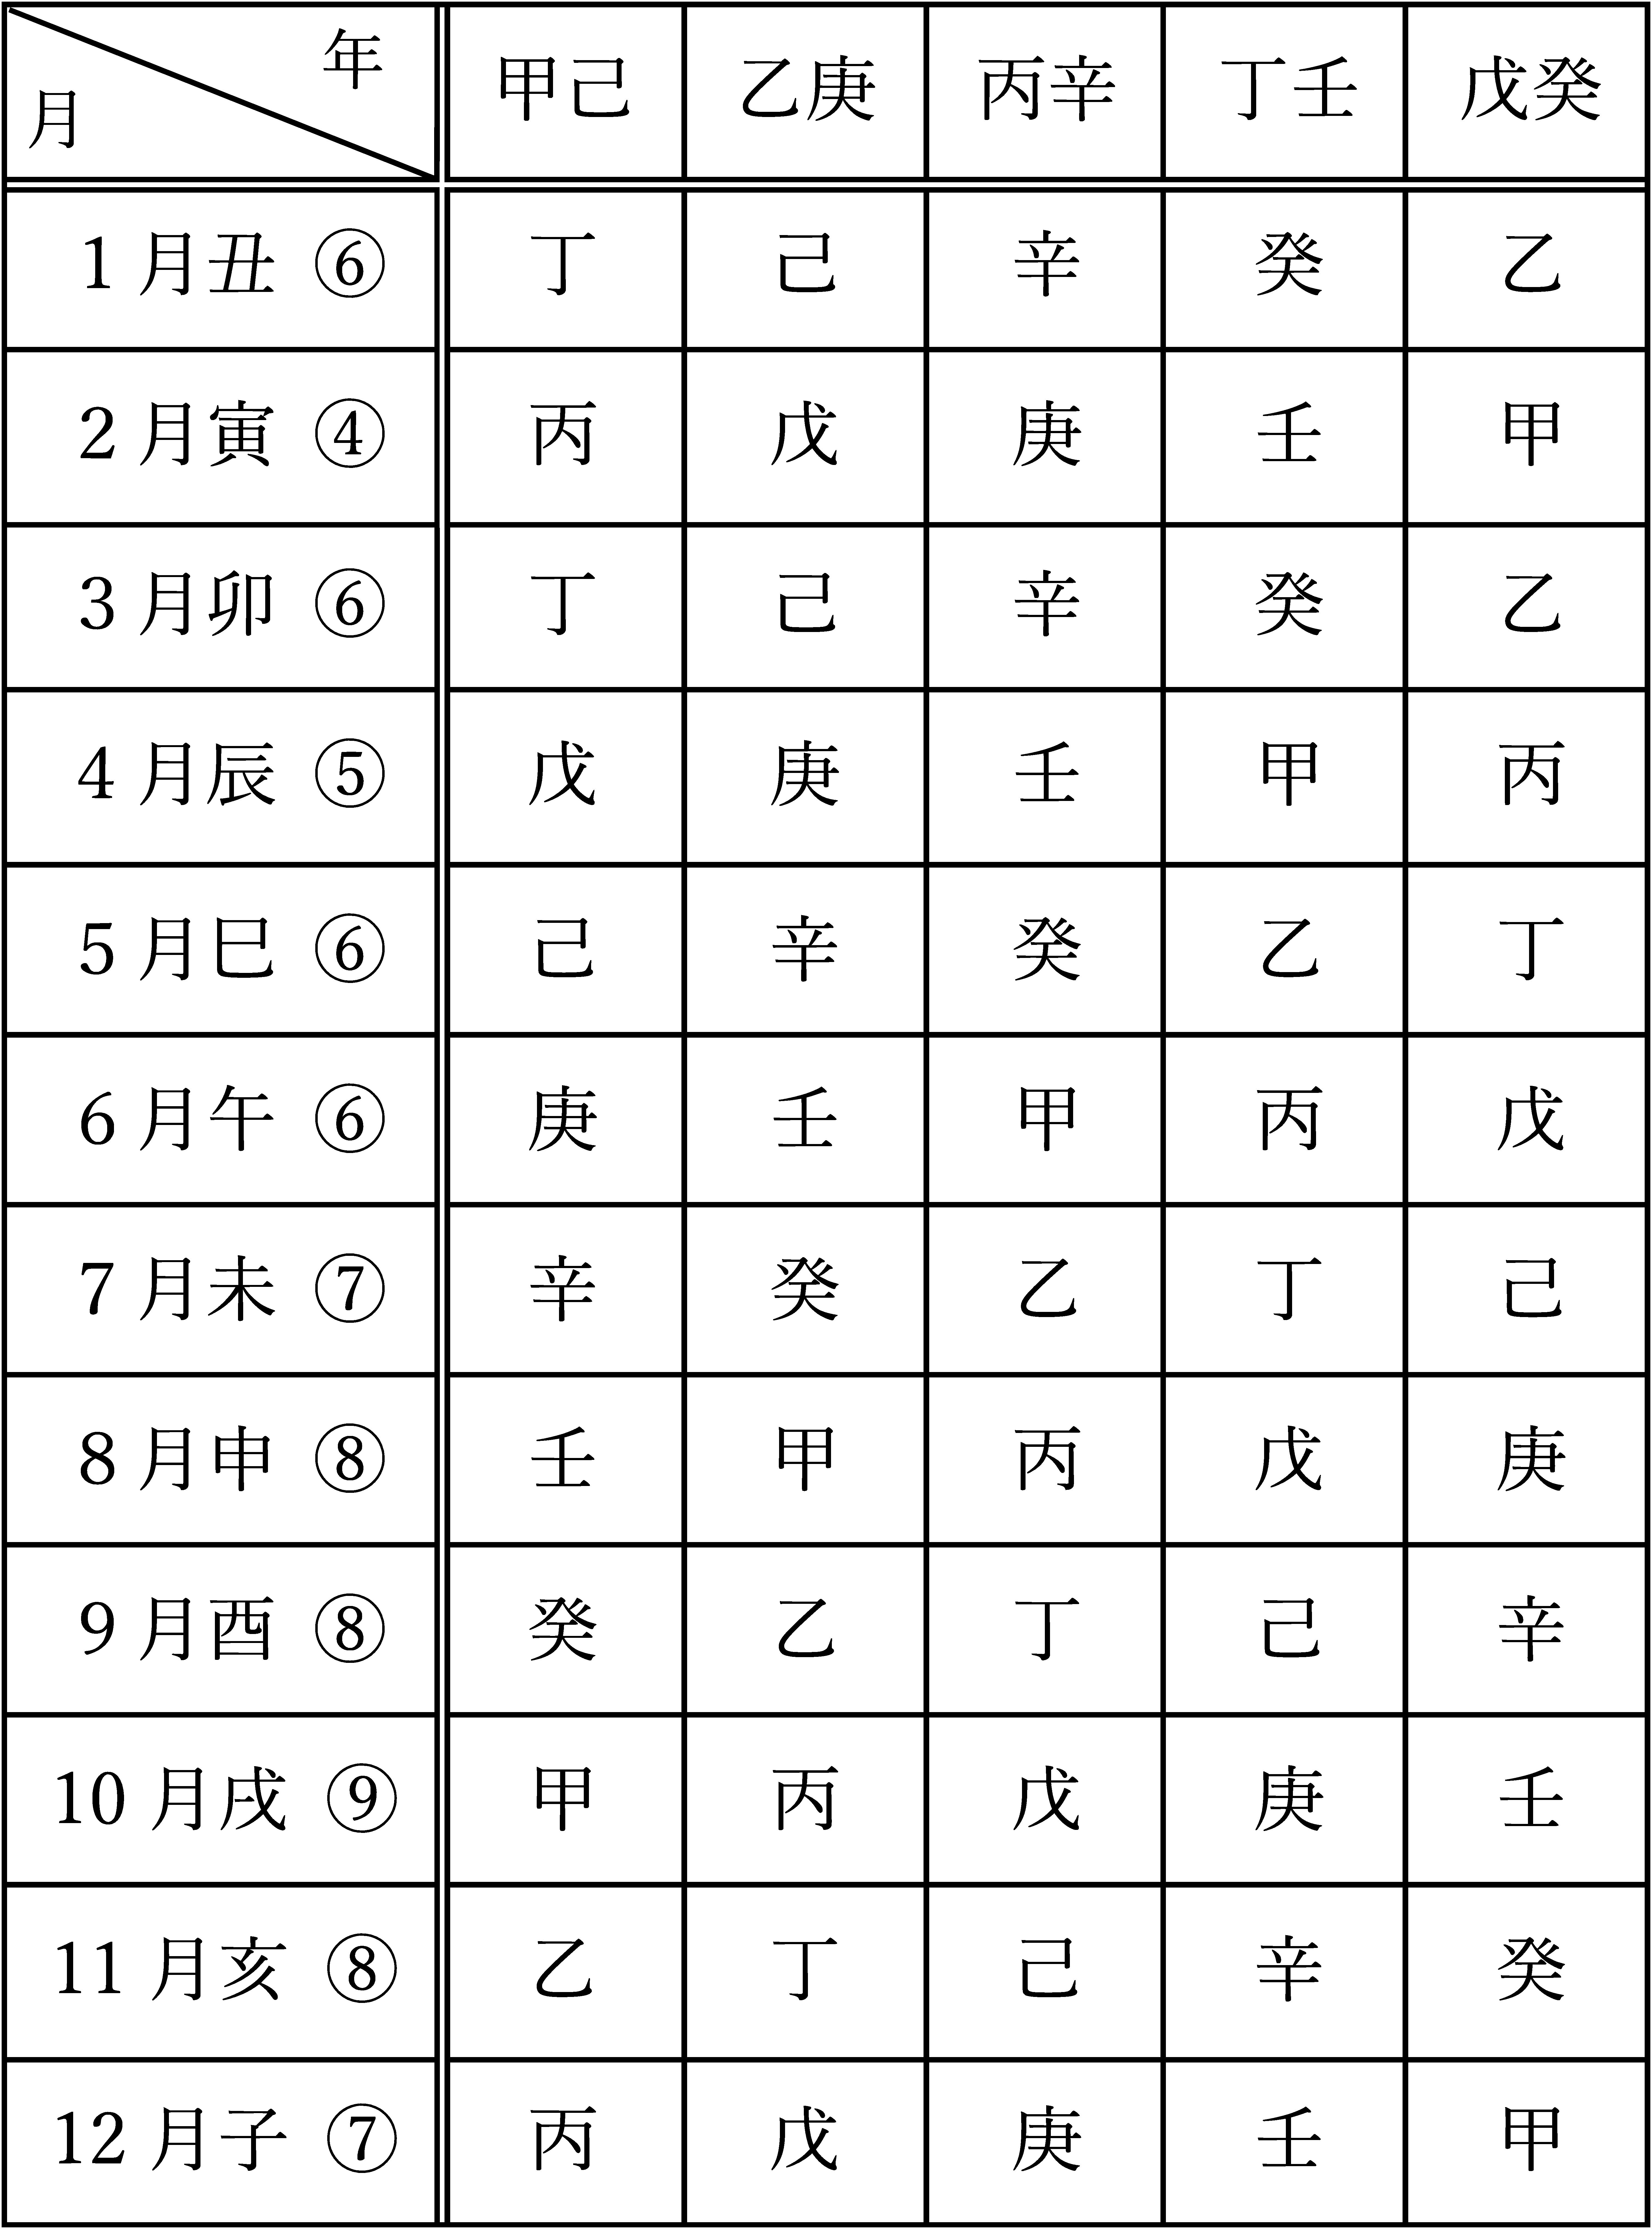
\includegraphics[width=75mm,angle=90]{figs/table3-1.eps}
\end{figure}

平成\rensuji{10}年\rensuji{11}月を例として説明します。

前述のとおり、年の干は「戊」でしたので、月干支表の「戊」の行を参照します。この表によれば、「戊」の「\rensuji{11}月亥」は「癸」です。そのため、平成\rensuji{10}年\rensuji{11}月の月干支は「癸亥」になります。

次に、昭和\rensuji{61}年9月を例として説明します。

六十干支表によれば、\rensuji{61}+2ー\rensuji{60}=3の干支は「丙寅」ですので、これが年干支になります。月干支表の「丙」の行において「9月酉」は「丁」です。そのため、昭和\rensuji{61}年9月の月干支は「丁酉」になります。

最後に、平成8年1月を例として説明します。

六十干支表によれば、8+5=\rensuji{13}の干支は「丙子」です。しかし、1月はまだ節入りしていないので、年干支はその前年の「乙亥」になります。月干支表の「乙」の行において「1月丑」は「己」です。そのため、平成8年1月の月干支は「己丑」になります。\\

月干支を求める場合も、毎月の節入りを考慮する必要があることに注意が必要です。つまり、毎月の節入り前までに誕生した人については、前月の干支を採用するということです。\footnote{毎月の節入りは、\ruby{小寒}{しょうかん}(1月6日頃)、\ruby{立春}{りっしゅん}(2月4日頃)、\ruby{啓蟄}{けいちつ}(3月6日頃)、\ruby{清明}{せいめい}(4月5日頃)、\ruby{立夏}{りっか}(5月6日頃)、\ruby{芒種}{ぼうしゅ}(6月6日頃)、\ruby{小暑}{しょうしょ}(7月7日頃)、\ruby{立秋}{りっしゅう}(8月8日頃)、\ruby{白露}{はくろ}(9月8日頃)、\ruby{寒露}{かんろ}(\rensuji{10}月9日頃)、\ruby{立冬}{りっとう}(\rensuji{11}月8日頃)、\ruby{大雪}{だいせつ}(\rensuji{12}月7日頃)です。それぞれの日付と正確な時刻については、「理科年表」で発表されています。}

この注意事項を、次の図を用いて説明します。

\begin{wrapfigure}{l}[0pt]{0.2\textwidth}
  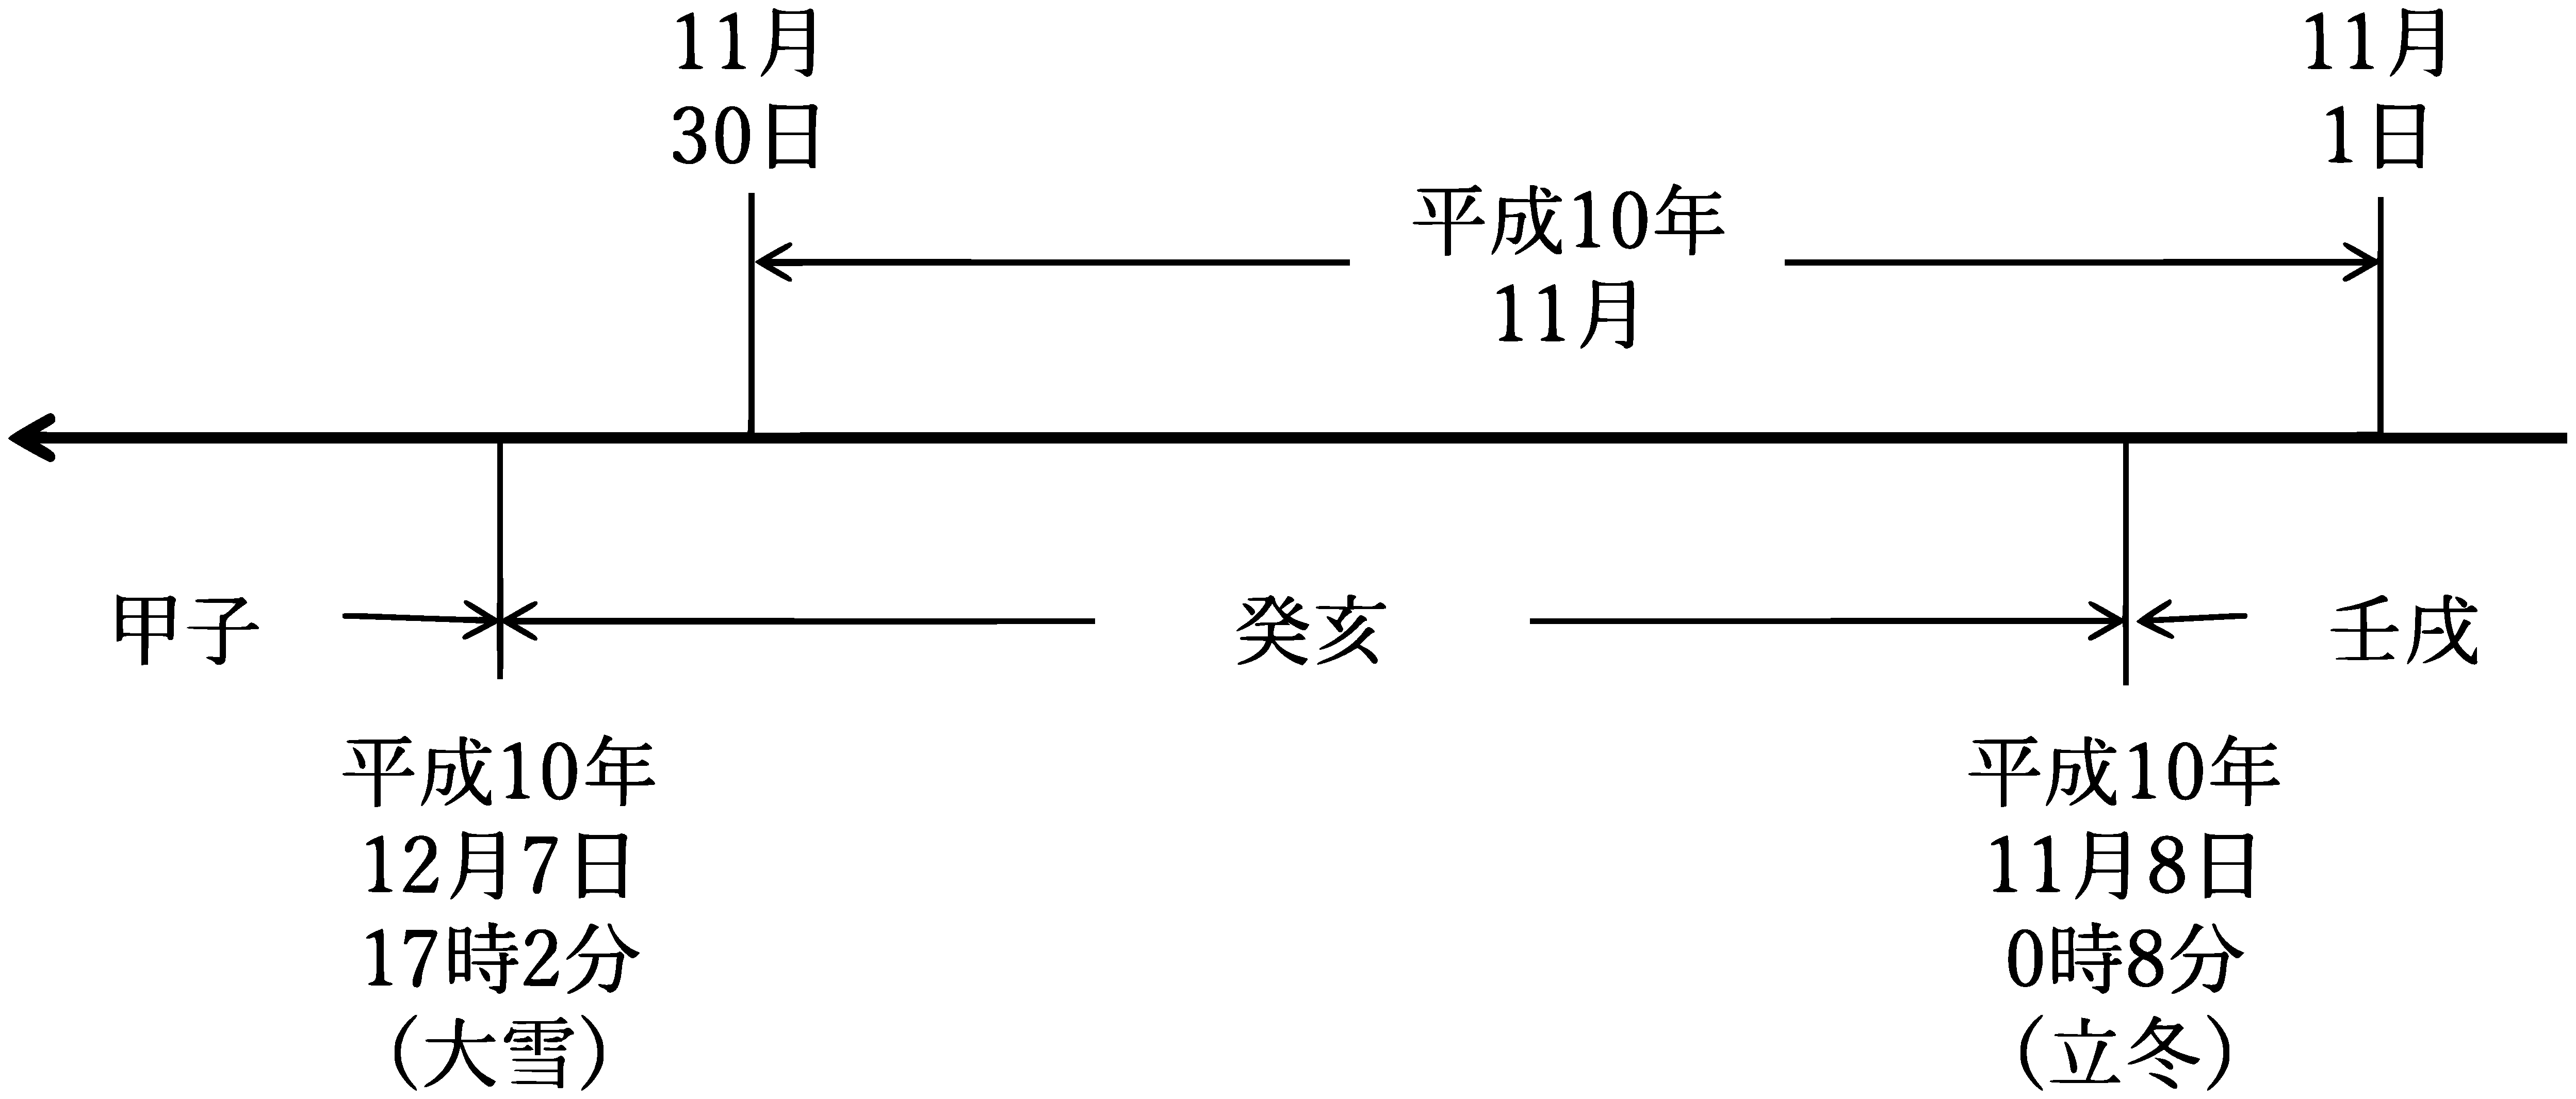
\includegraphics[width=75mm,angle=90]{figs/figure3-3.eps}
\end{wrapfigure}

一般に、平成\rensuji{10}年\rensuji{11}月は、\rensuji{11}月1日から\rensuji{11}月\rensuji{30}日までのことです。

一方で、四柱推命学では、平成\rensuji{10}年\rensuji{11}月「癸亥」の月柱を採用するのは、平成\rensuji{10}年\rensuji{11}月8日0時8分の節入り(立冬)から、同年\rensuji{12}月7日\rensuji{17}時2分の節入り(大雪)より前までです。

例えば、平成\rensuji{10}年\rensuji{11}月5日は、まだ「癸亥」には節入りしていませんので、その前月の「壬戌」を採用します。同様に、同年\rensuji{12}月2日は、まだ「甲子」に節入りしていませんので、「癸亥」を採用します。

このように、各月の上旬に生まれた人の月柱の求め方は変則的になるので、注意が必要です。

なお、月干支表の○内数字は「標準節入日」です。例えば、毎年8月の節入り(立秋)は、正確な時刻は別として「だいたい8日」です。そのため、「8月申」の下に「\textcircled{\rensuji{8}}」と記載しています。

この標準節入日を参考にして、節入りの有無を大まかに検討し、当月の干支を採用するか、前月の干支を採用するかを判断すればよいでしょう。


\subsubsection*{日の干支の求め方}

日干支は、次の生日基数表を用いて求めます。

\begin{figure}[h]
  \centering
  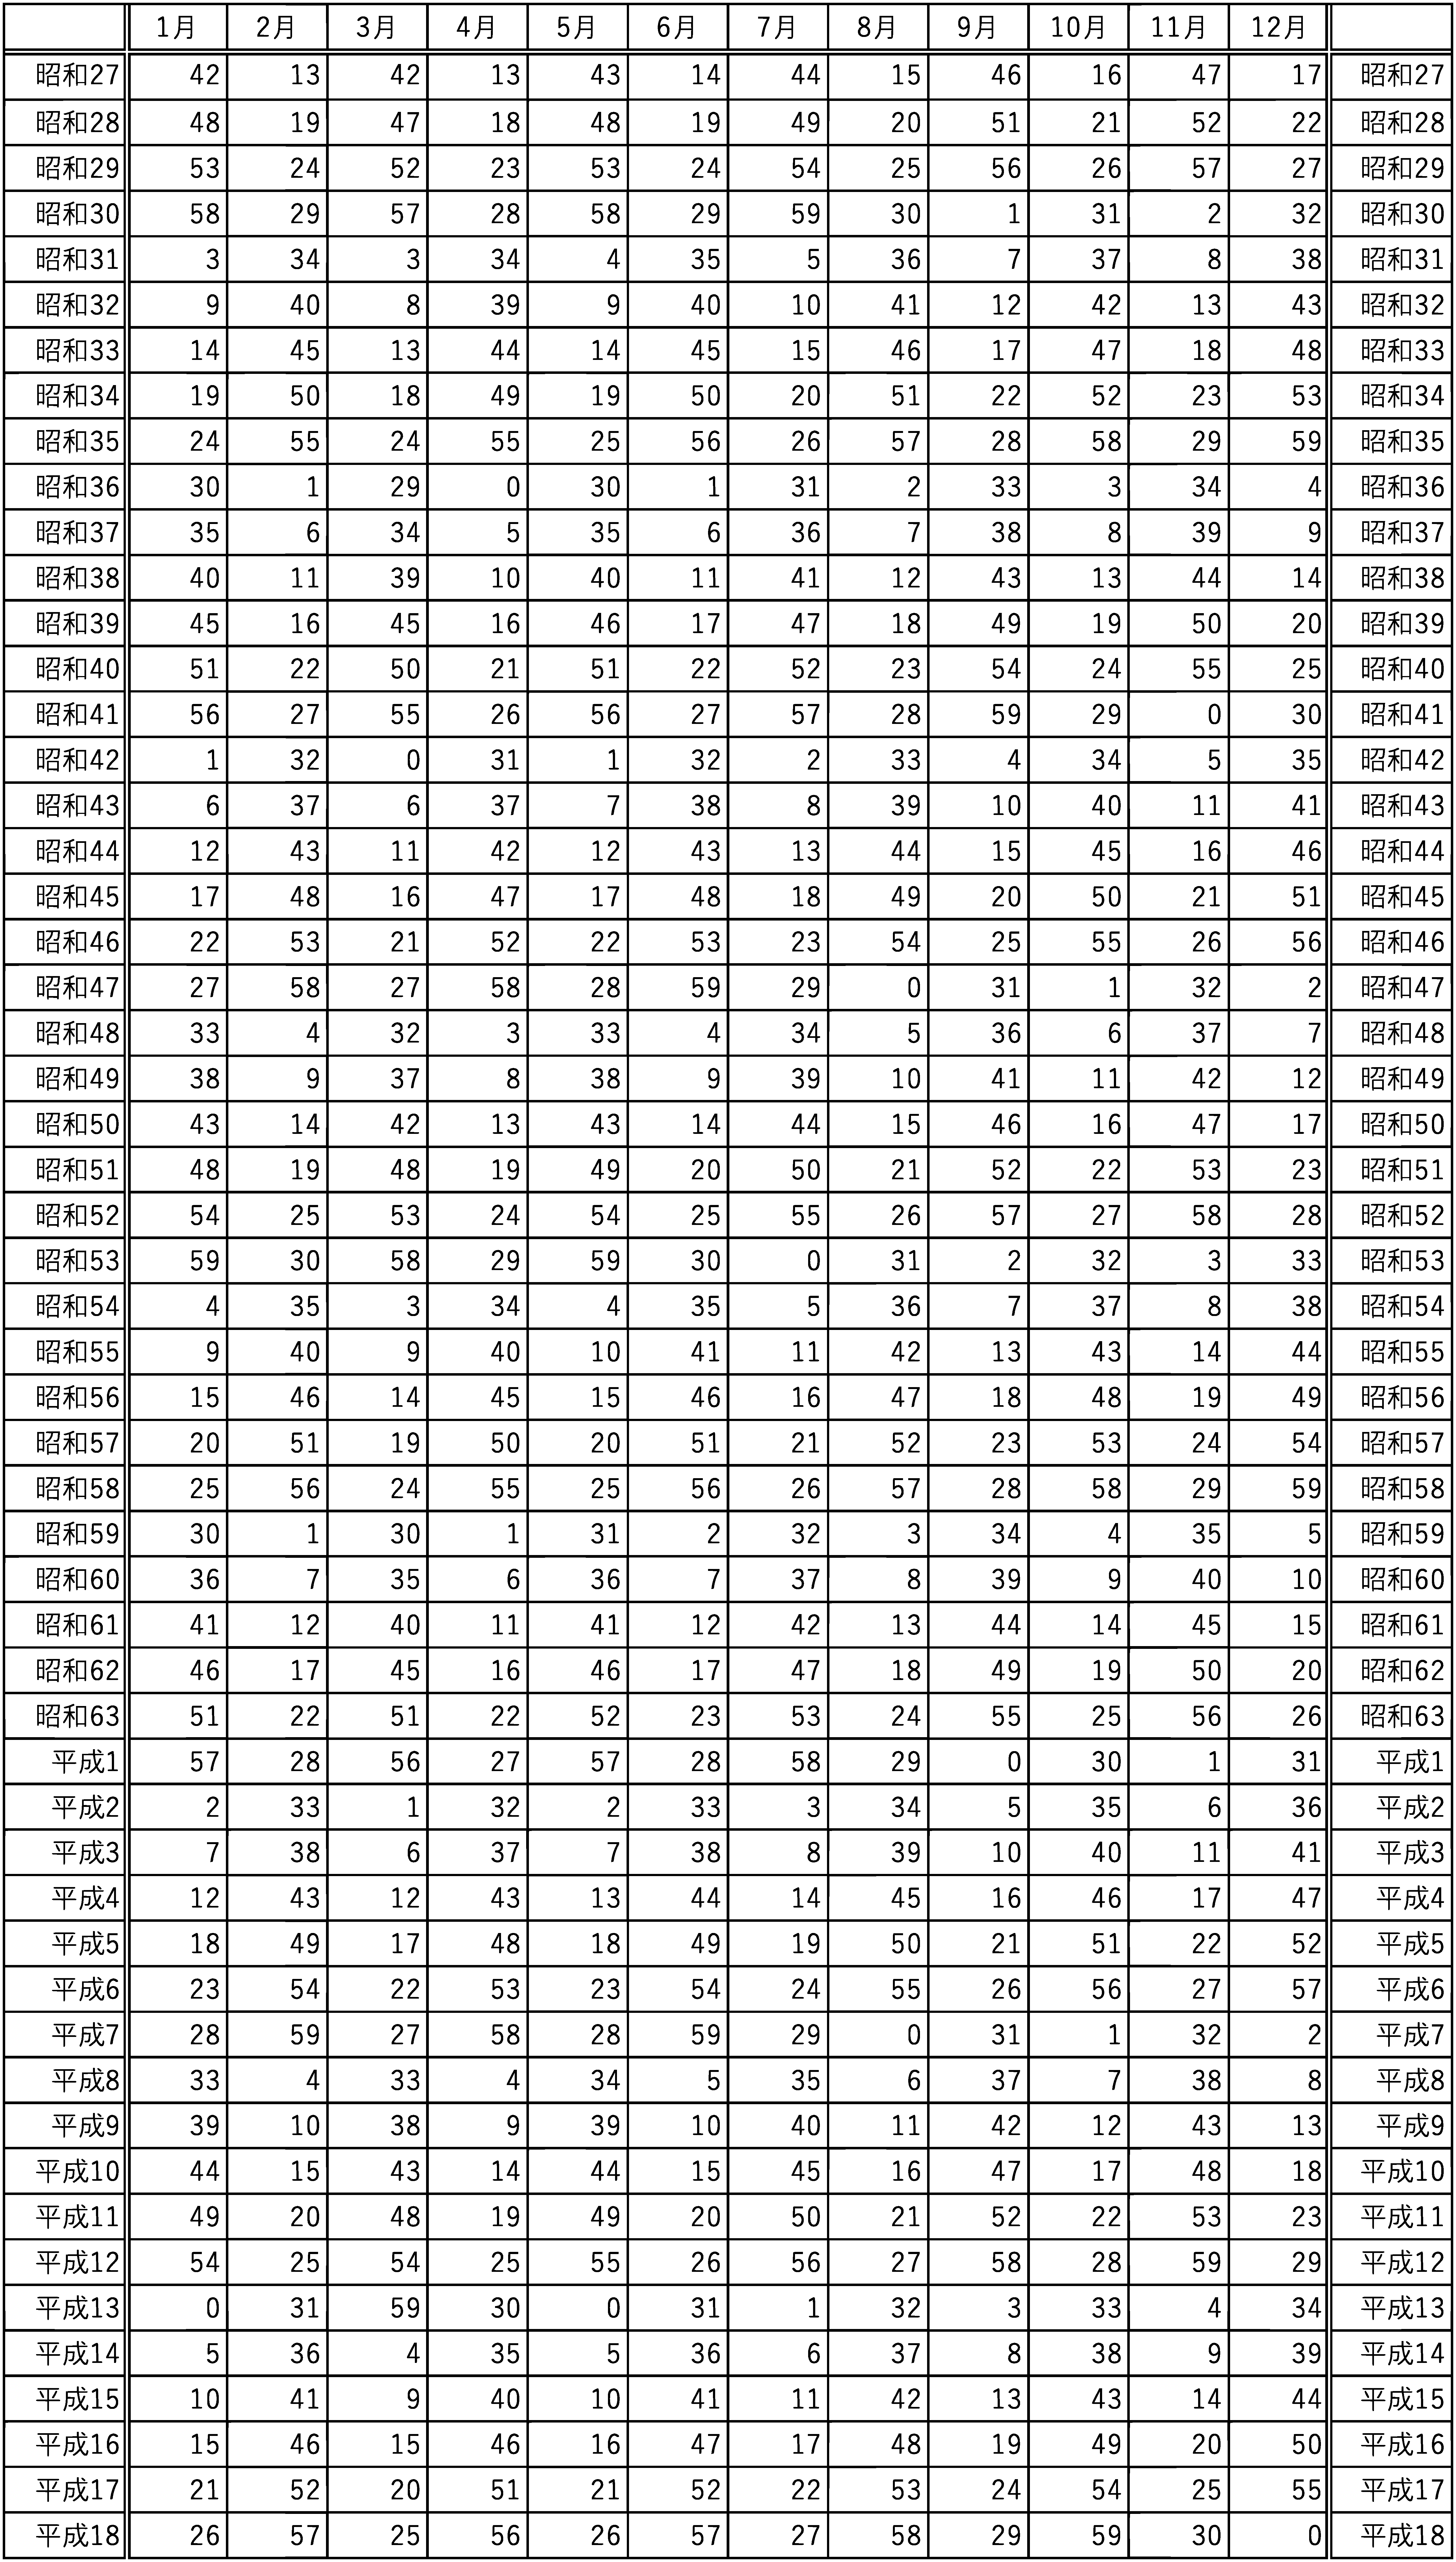
\includegraphics[width=75mm,angle=90]{figs/table3-2-1.eps}
\end{figure}

\clearpage

\begin{figure}[h]
  \centering
  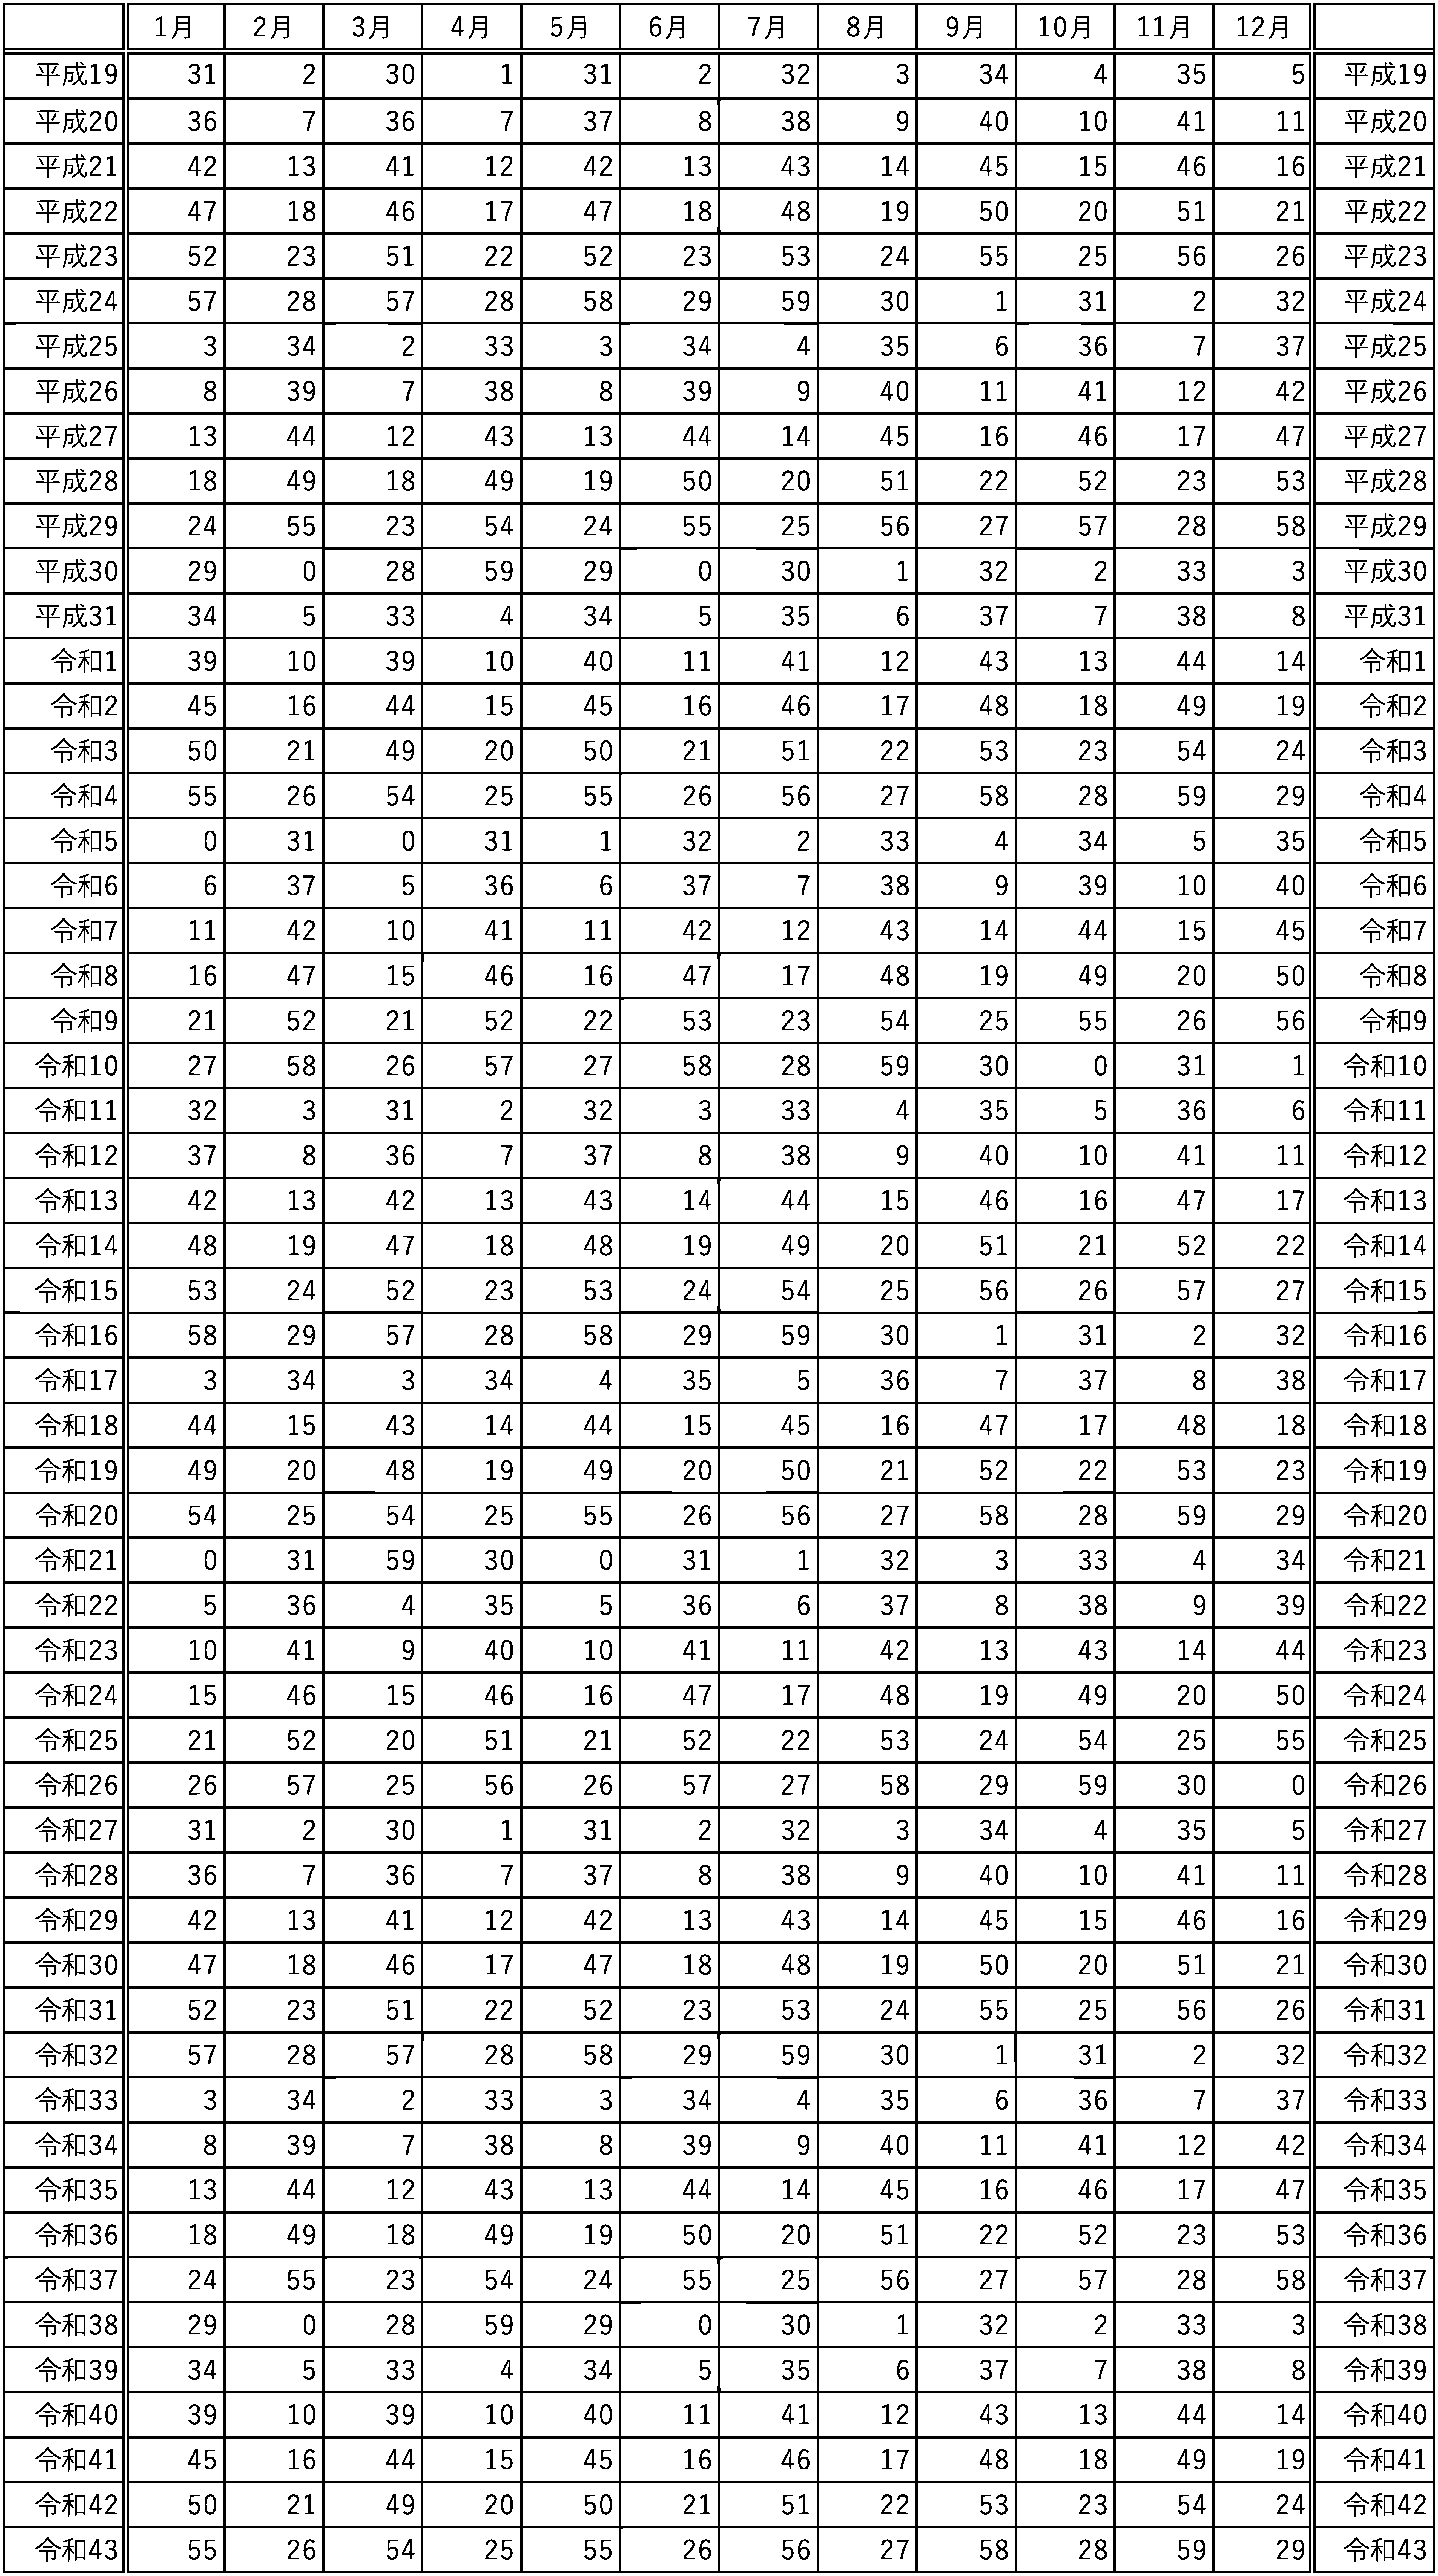
\includegraphics[width=75mm,angle=90]{figs/table3-2-2.eps}
\end{figure}

日干支を求める手順は、次のとおりです。

\begin{enumerate}
\item 生日基数表から年月に対応する基数を得る
\item その基数に日の数を足す(足した数が\rensuji{60}を超過している場合は\rensuji{60}を引く)
\item 足した数に対応する干支を六十干支表から得る
\end{enumerate}

平成\rensuji{10}年\rensuji{11}月\rensuji{10}日を例として説明します。

生日基数表によれば、平成\rensuji{10}年\rensuji{11}月に対応する基数は「\rensuji{48}」です。これに日数(\rensuji{10})を足すと「\rensuji{58}」です。六十干支表において「\rensuji{58}」に対応する干支は「辛酉」ですので、平成\rensuji{10}年\rensuji{11}月\rensuji{10}日の干支は「辛酉」になります。

次に、昭和\rensuji{61}年9月\rensuji{27}日を例として説明します。

生日基数表によれば、昭和\rensuji{61}年9月に対応する基数は「\rensuji{44}」です。これに日数(\rensuji{27})を足すと「\rensuji{71}」です。\rensuji{60}を超えているので、\rensuji{71}から\rensuji{60}を引いて\rensuji{11}を得ます。六十干支表において「\rensuji{11}」に対応する干支は「甲戌」ですので、昭和\rensuji{61}年9月\rensuji{27}日の干支は「甲戌」になります。


\subsubsection*{時の干支の求め方}

時の干支は、次の時干支表を用いて求めます。

\begin{figure}[h]
  \centering
  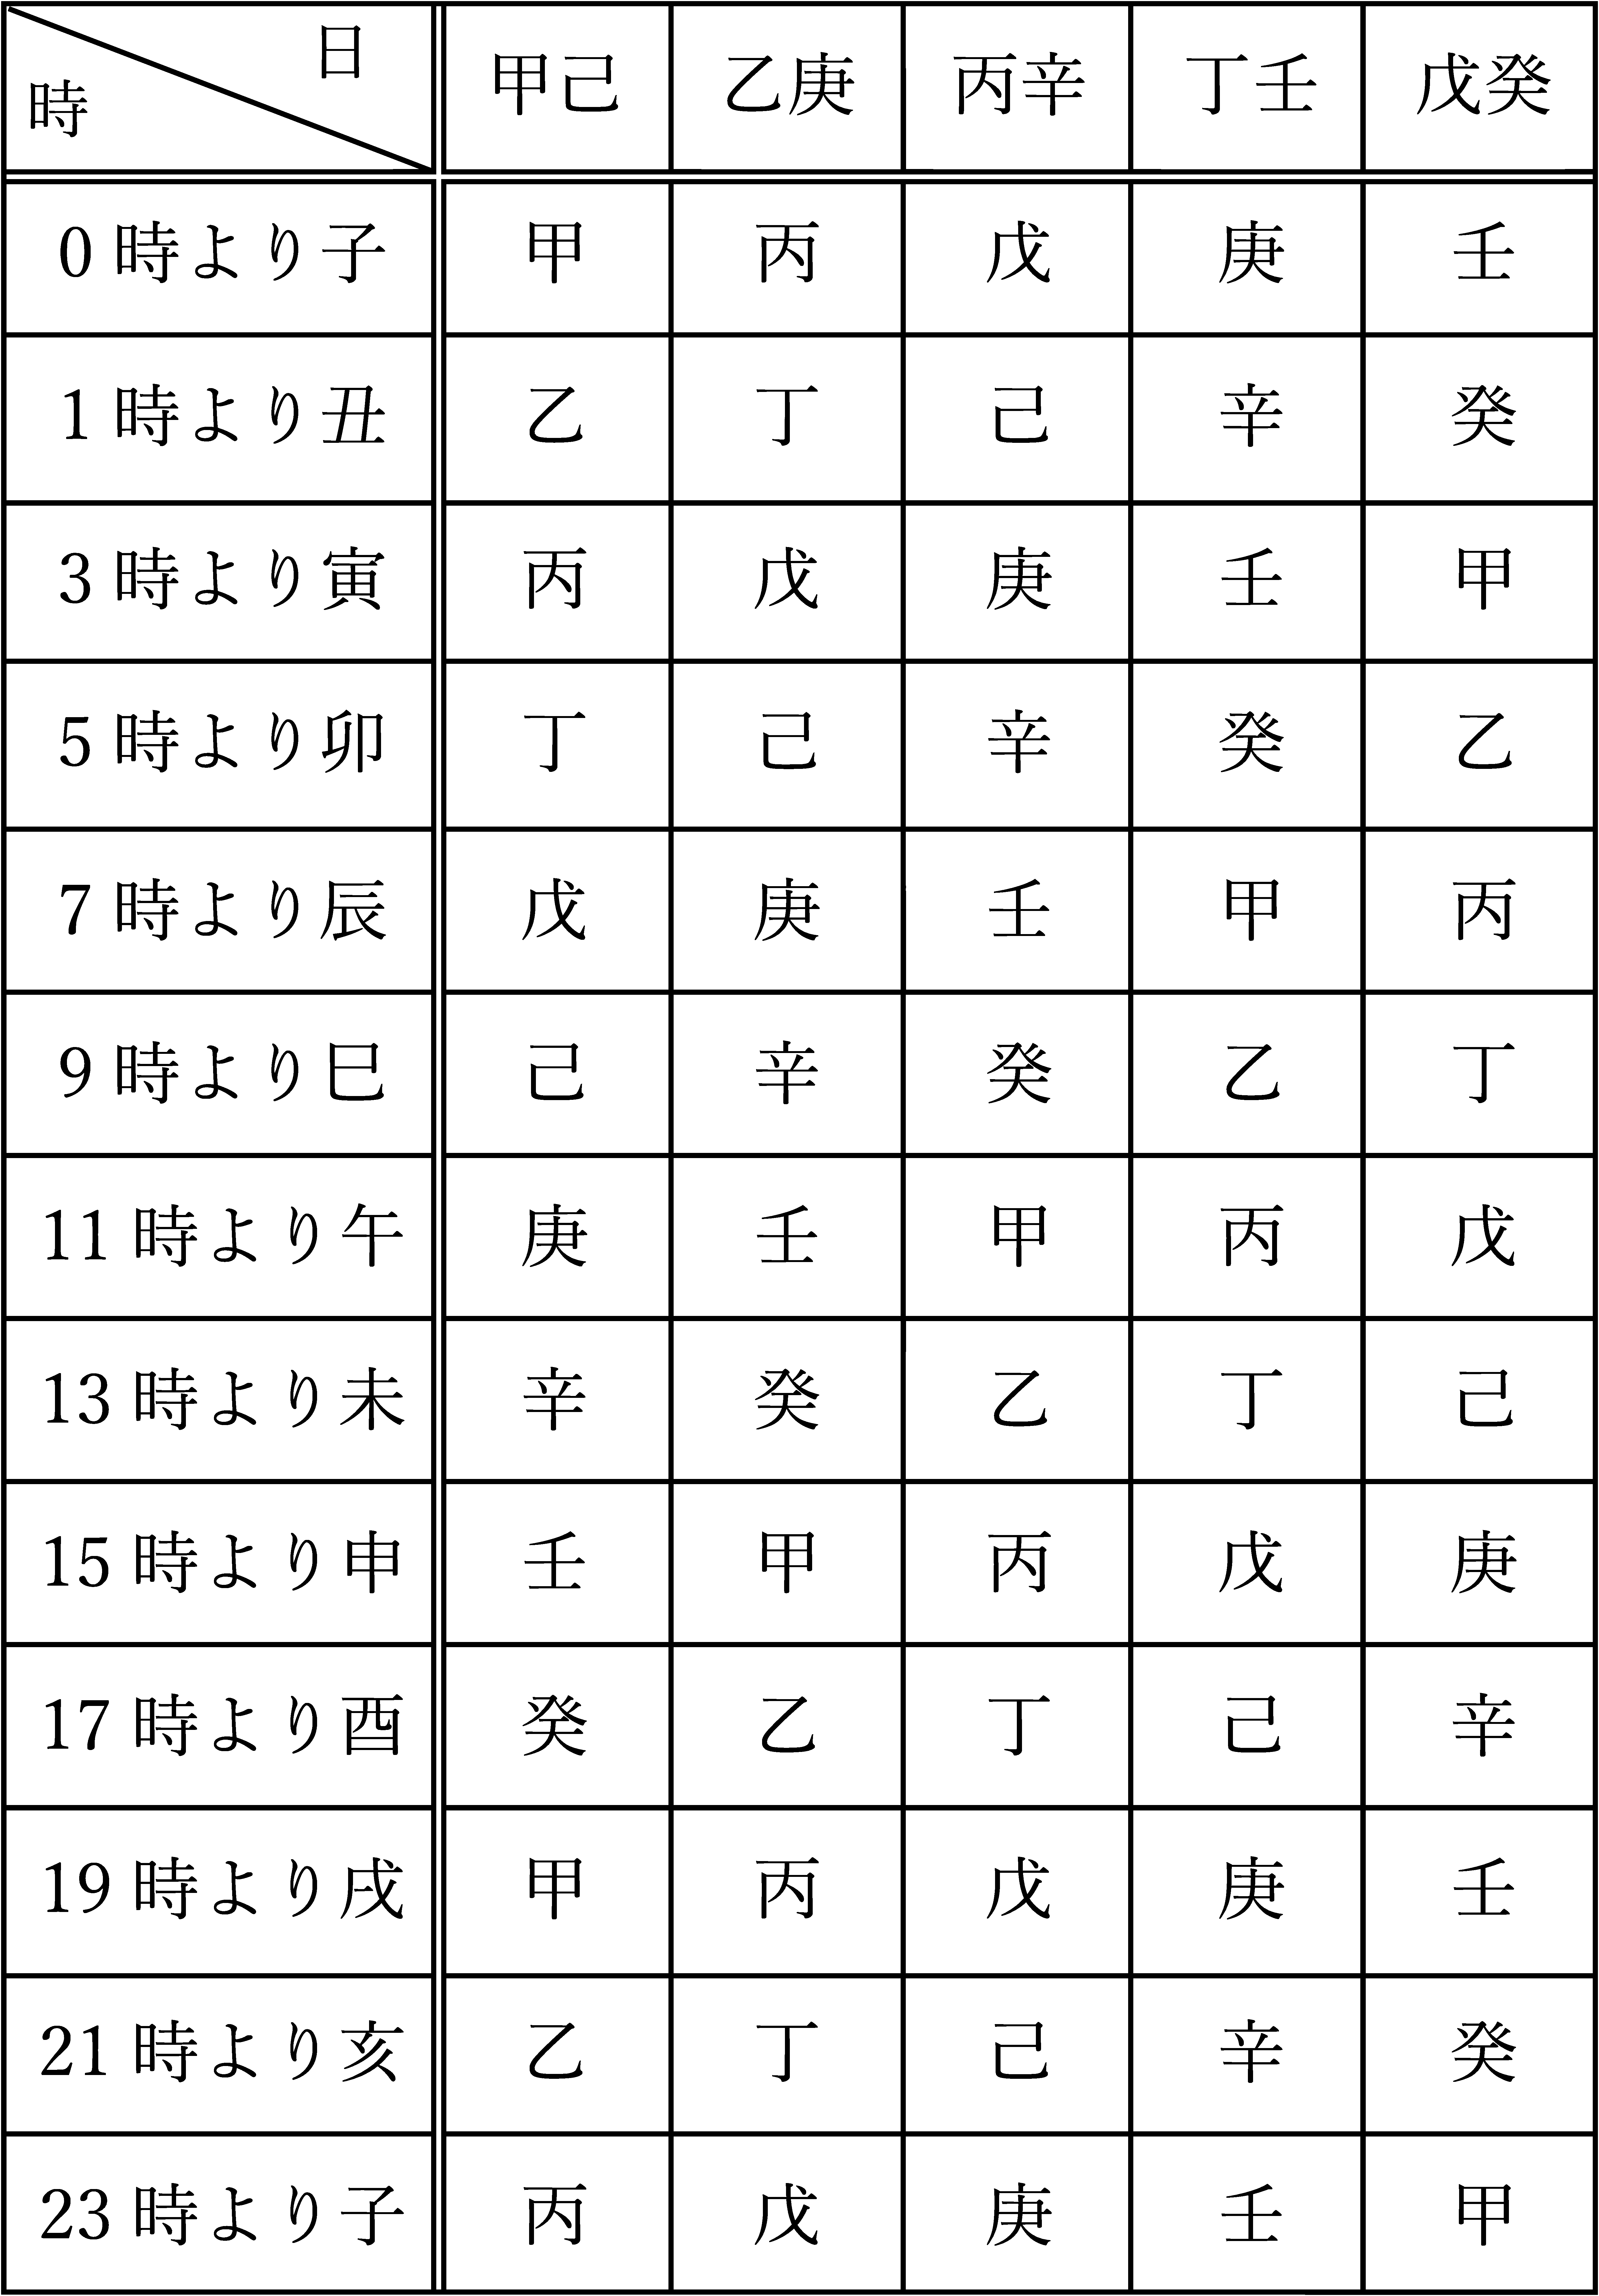
\includegraphics[width=75mm,angle=90]{figs/table3-3.eps}
\end{figure}

平成\rensuji{10}年\rensuji{11}月\rensuji{10}日\rensuji{13}時\rensuji{45}分を例として説明します。

前述のとおり、日干は「辛」でしたので、時干支表の「辛」の行を参照します。この表によれば、「辛」の「\rensuji{13}時より未」は「乙」です。そのため、平成\rensuji{10}年\rensuji{11}月\rensuji{10}日\rensuji{13}時\rensuji{45}分の時干支は「乙未」になります。

次に、昭和\rensuji{61}年9月\rensuji{27}日8時\rensuji{51}分を例として説明します。

前述のとおり、日干は「甲」でしたので、時干支表の「甲」の行を参照します。この表によれば、「甲」の「7時より辰」は「戊」です。そのため、昭和\rensuji{61}年9月\rensuji{27}日8時\rensuji{51}分の時干支は「戊辰」になります。

\subsubsection*{四柱干支の求め方のまとめ}
4つの例題をとおして、四柱干支の求め方をまとめましょう。\\

\noindent
(1) 昭和\rensuji{58}年(1983年)8月\rensuji{21}日\rensuji{14}時\rensuji{13}分

まず、六十干支表から昭和\rensuji{58}+2=\rensuji{60}で年干支「癸亥」を得ます。次に、月干支表の「癸」の行を参照すると、「8月申」は「庚」です。ここから月干支「庚申」を得ます。

\begin{wrapfigure}{l}[0pt]{0.2\textwidth}
  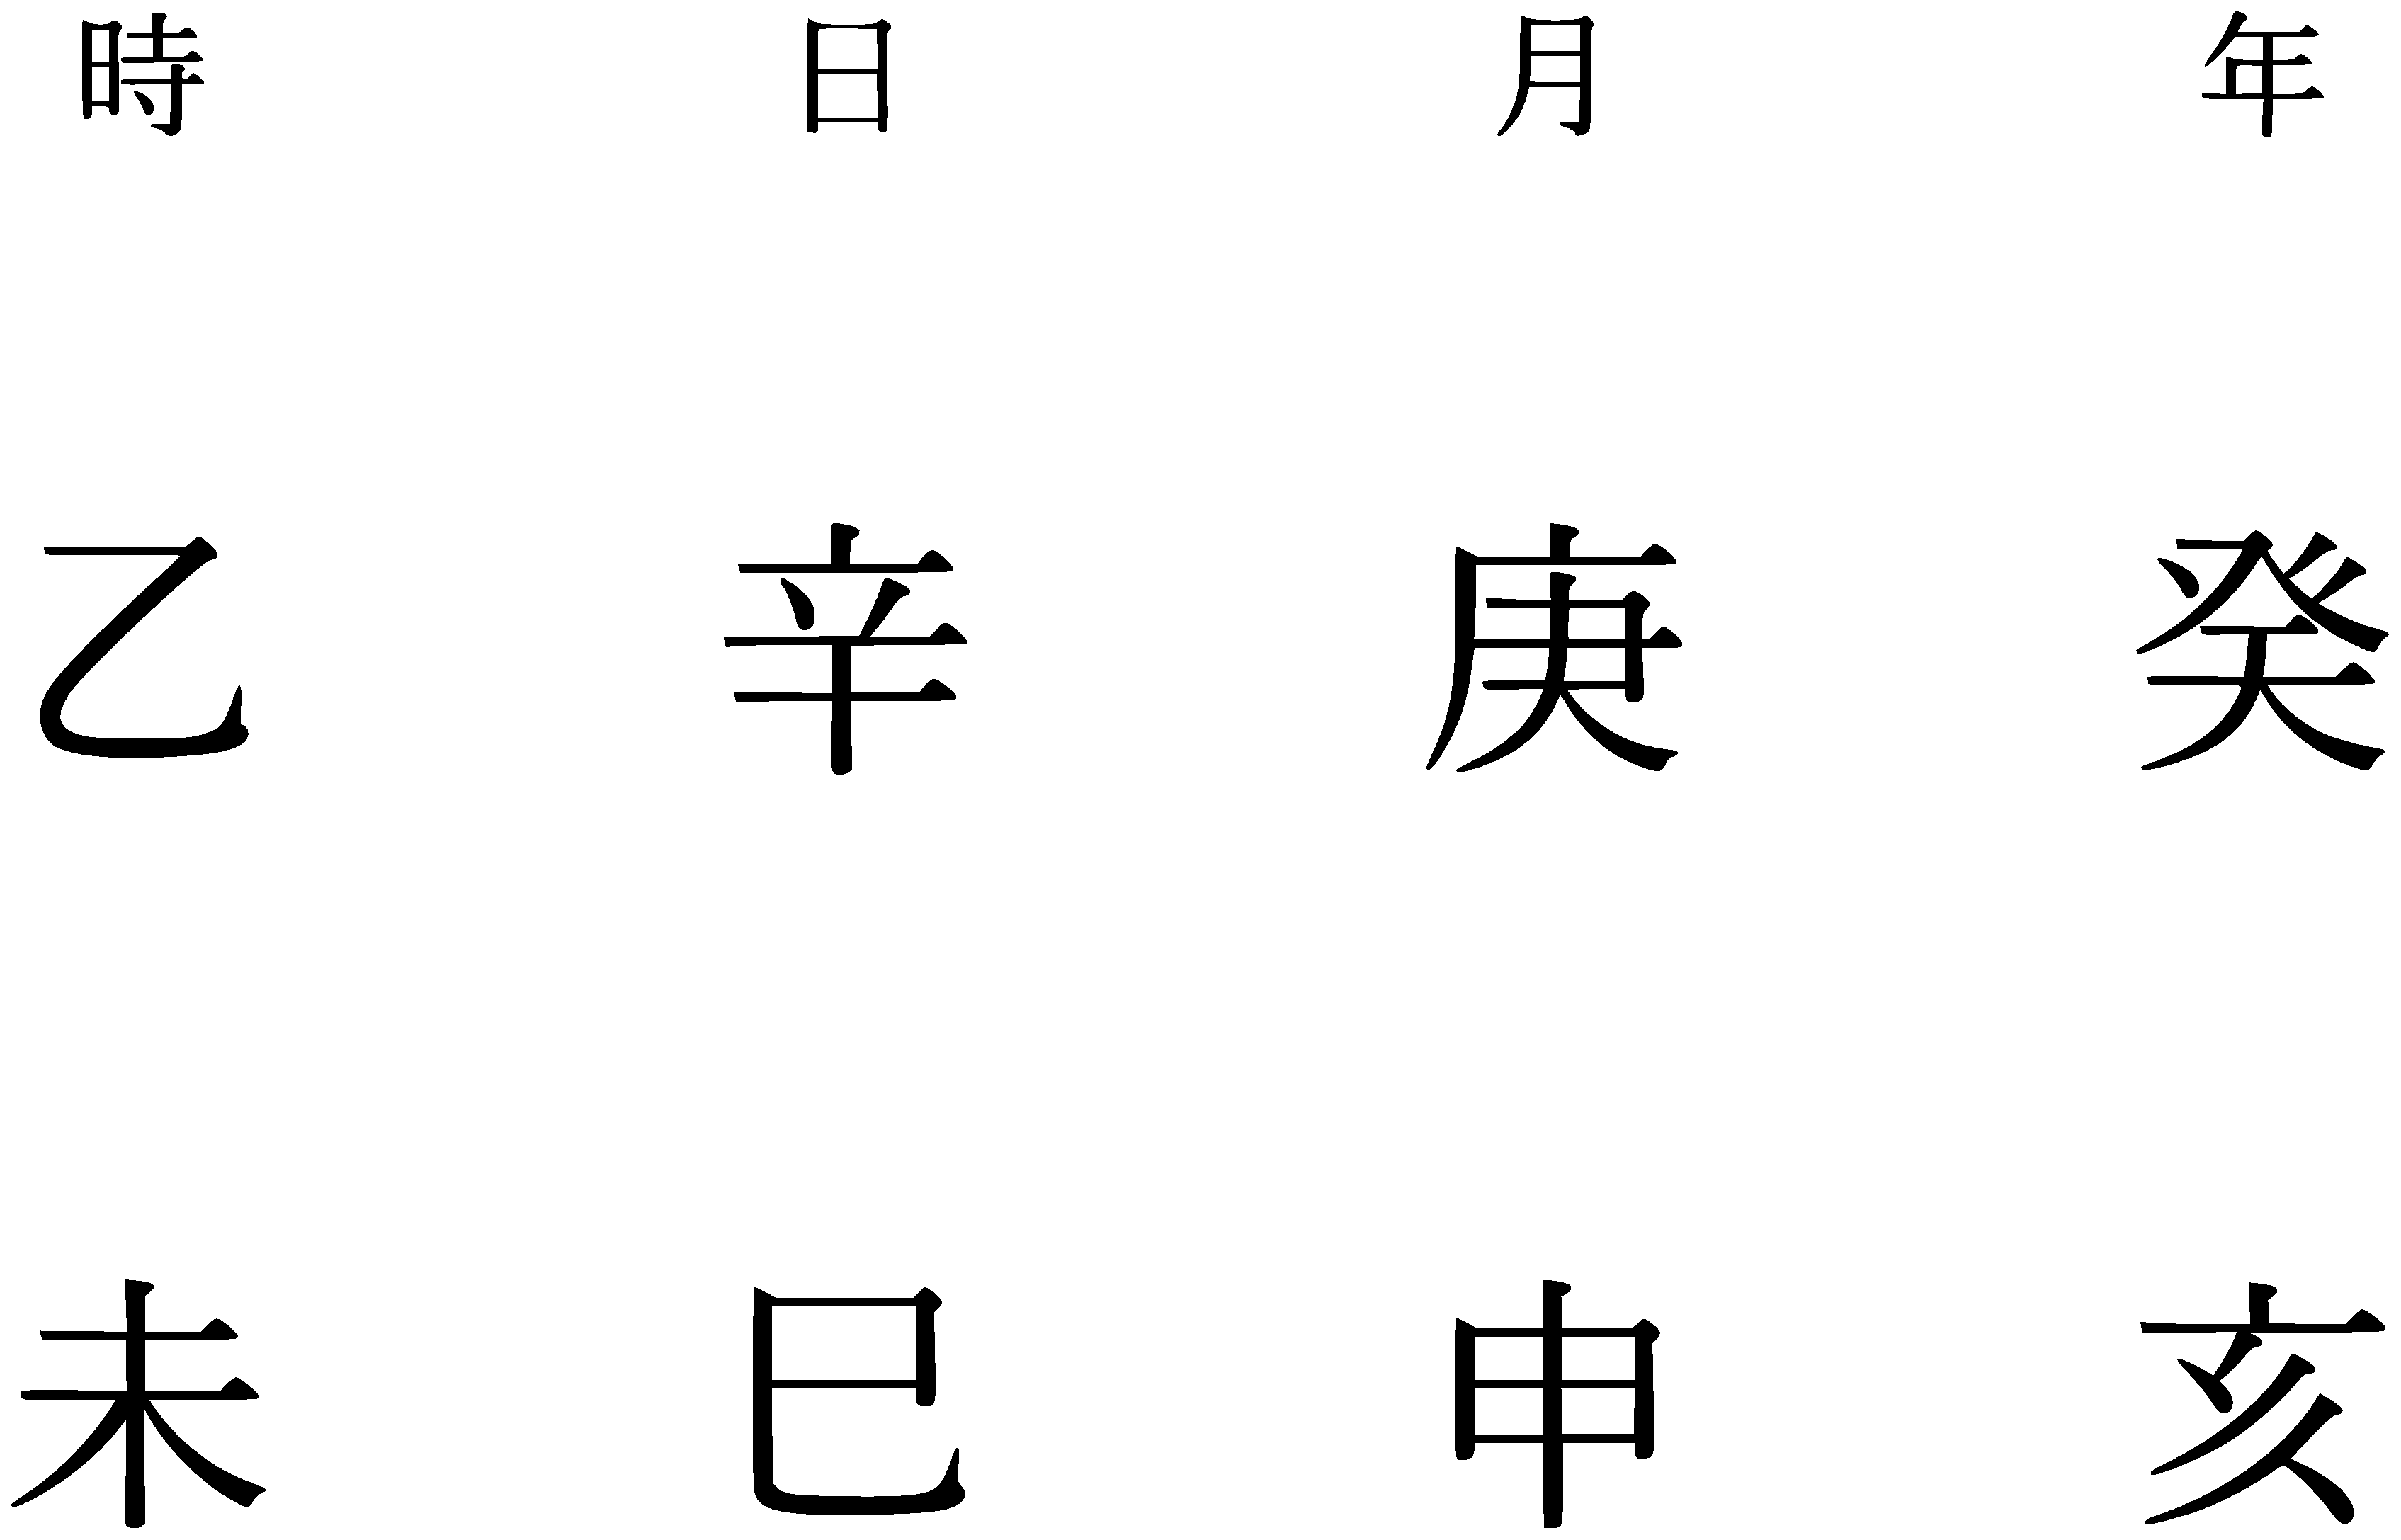
\includegraphics[width=50mm,angle=90]{figs/figure3-4.eps}
\end{wrapfigure}

生日基数表によれば、昭和\rensuji{58}年8月に対応する基数は「\rensuji{57}」ですので、\rensuji{57}+\rensuji{21}ー\rensuji{60}=\rensuji{18}です。六十干支表において「\rensuji{18}」に対応する干支は「辛巳」ですので、これが日干支になります。最後に、時干支表の「辛」の行を参照すると、「\rensuji{13}時より未」は「乙」です。そのため、ここから時干支「乙未」を得ます。

まとめると、昭和\rensuji{58}年8月\rensuji{21}日\rensuji{14}時\rensuji{13}分生まれの四柱干支は、上のとおりです。\\

\noindent
(2) 平成7年(1995年)1月\rensuji{27}日9時\rensuji{21}分

まず、六十干支表から平成7+5=\rensuji{12}で年干支「乙亥」を得ます。しかし、1月はまだ節入りしていないため、前年の「甲戌」が年干支となります。次に、月干支表の「甲」の行を参照すると、「1月丑」は「丁」です。ここから月干支「丁丑」を得ます。

生日基数表によれば、平成7年1月に対応する基数は「\rensuji{28}」ですので、\rensuji{28}+\rensuji{27}=\rensuji{55}です。六十干支表において「\rensuji{55}」に対応する干支は「戊午」ですので、これが日干支になります。最後に、時干支表の「戊」の行を参照すると、「9時より巳」は「丁」です。そのため、ここから時干支「丁巳」を得ます。

まとめると、平成7年1月\rensuji{27}日9時\rensuji{21}分生まれの四柱干支は、次のとおりです。

\begin{figure}[h]
  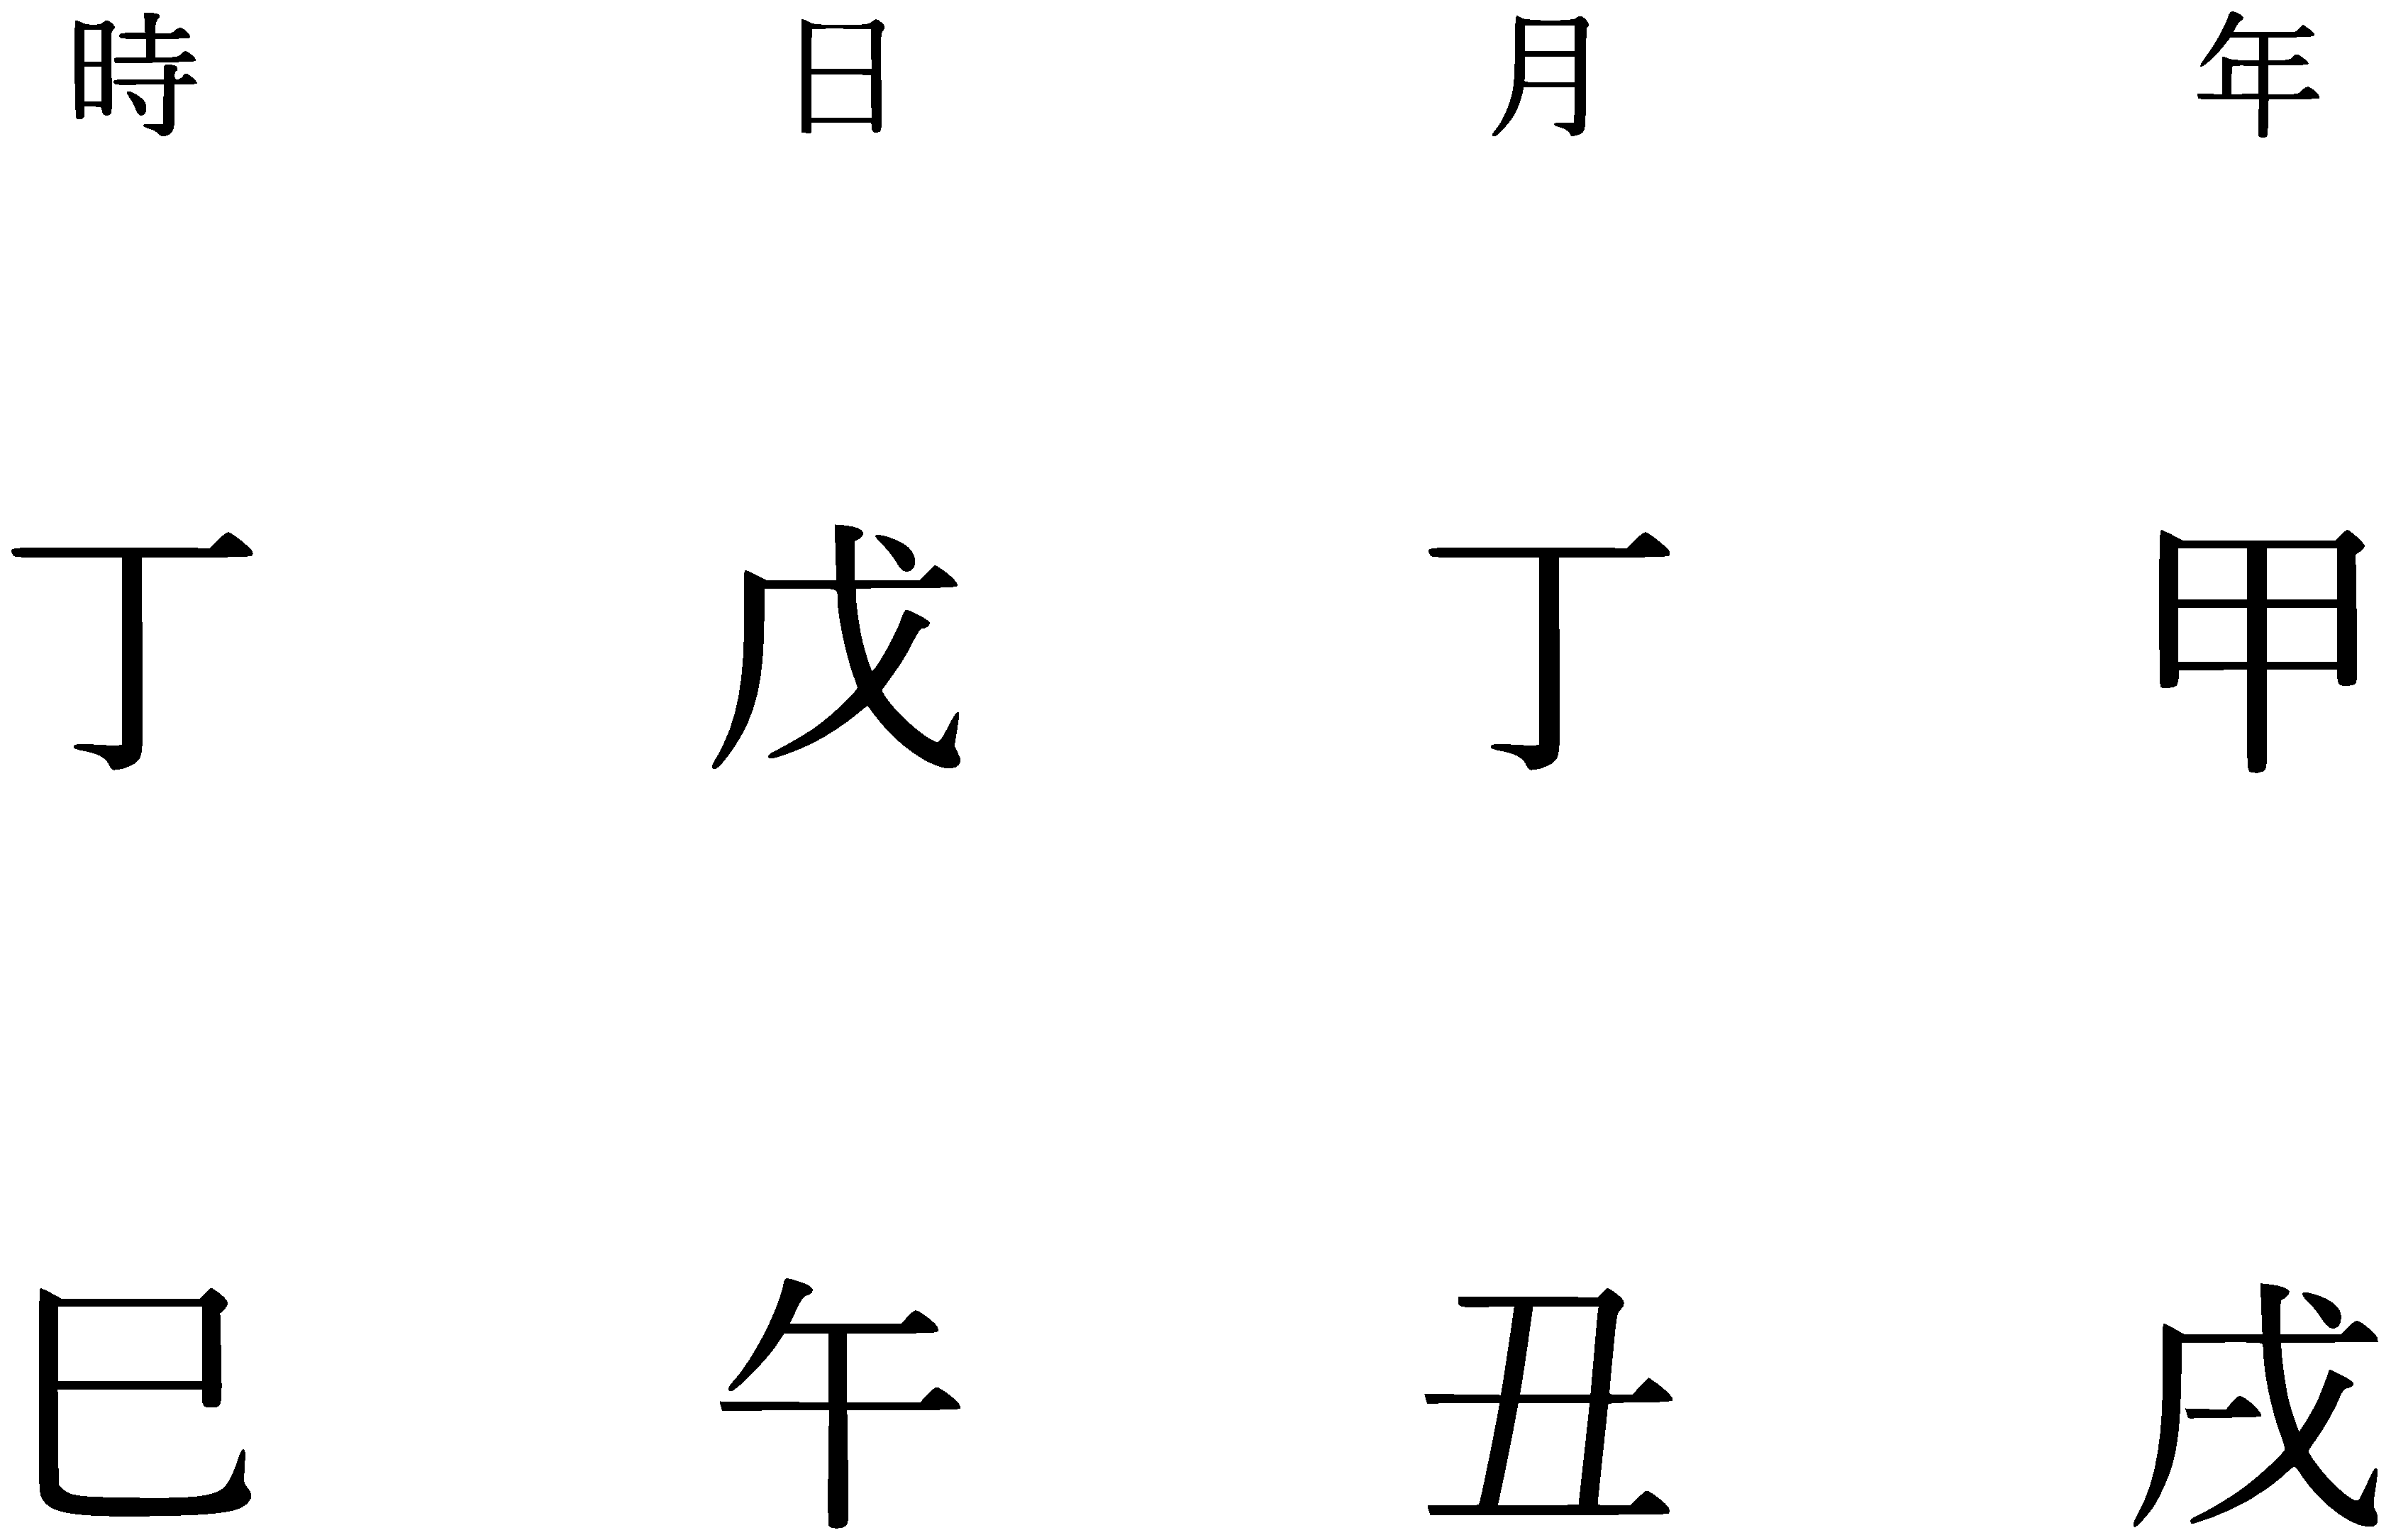
\includegraphics[width=45mm,angle=90]{figs/figure3-5.eps}
\end{figure}

\noindent
\\(3) 平成9年(1997年)6月3日\rensuji{21}時\rensuji{22}分

まず、六十干支表から平成9+5=\rensuji{14}で年干支「丁丑」を得ます。次に、6月の標準節入日を参照すると「6日」であるため、6月3日はまだ節入りしていないことが分かります。そのため、月干支表の「丁」の行における「5月巳」を参照し、「乙」を得ます。月干支は「乙巳」です。

生日基数表によれば、平成9年6月に対応する基数は「\rensuji{10}」ですので、\rensuji{10}+3=\rensuji{13}です。六十干支表において「\rensuji{13}」に対応する干支は「丙子」ですので、これが日干支になります。最後に、時干支表の「丙」の行を参照すると、「\rensuji{21}時より亥」は「己」です。そのため、ここから時干支「己亥」を得ます。

まとめると、平成9年6月3日\rensuji{21}時\rensuji{22}分生まれの四柱干支は、次のとおりです。

\begin{figure}[h]
  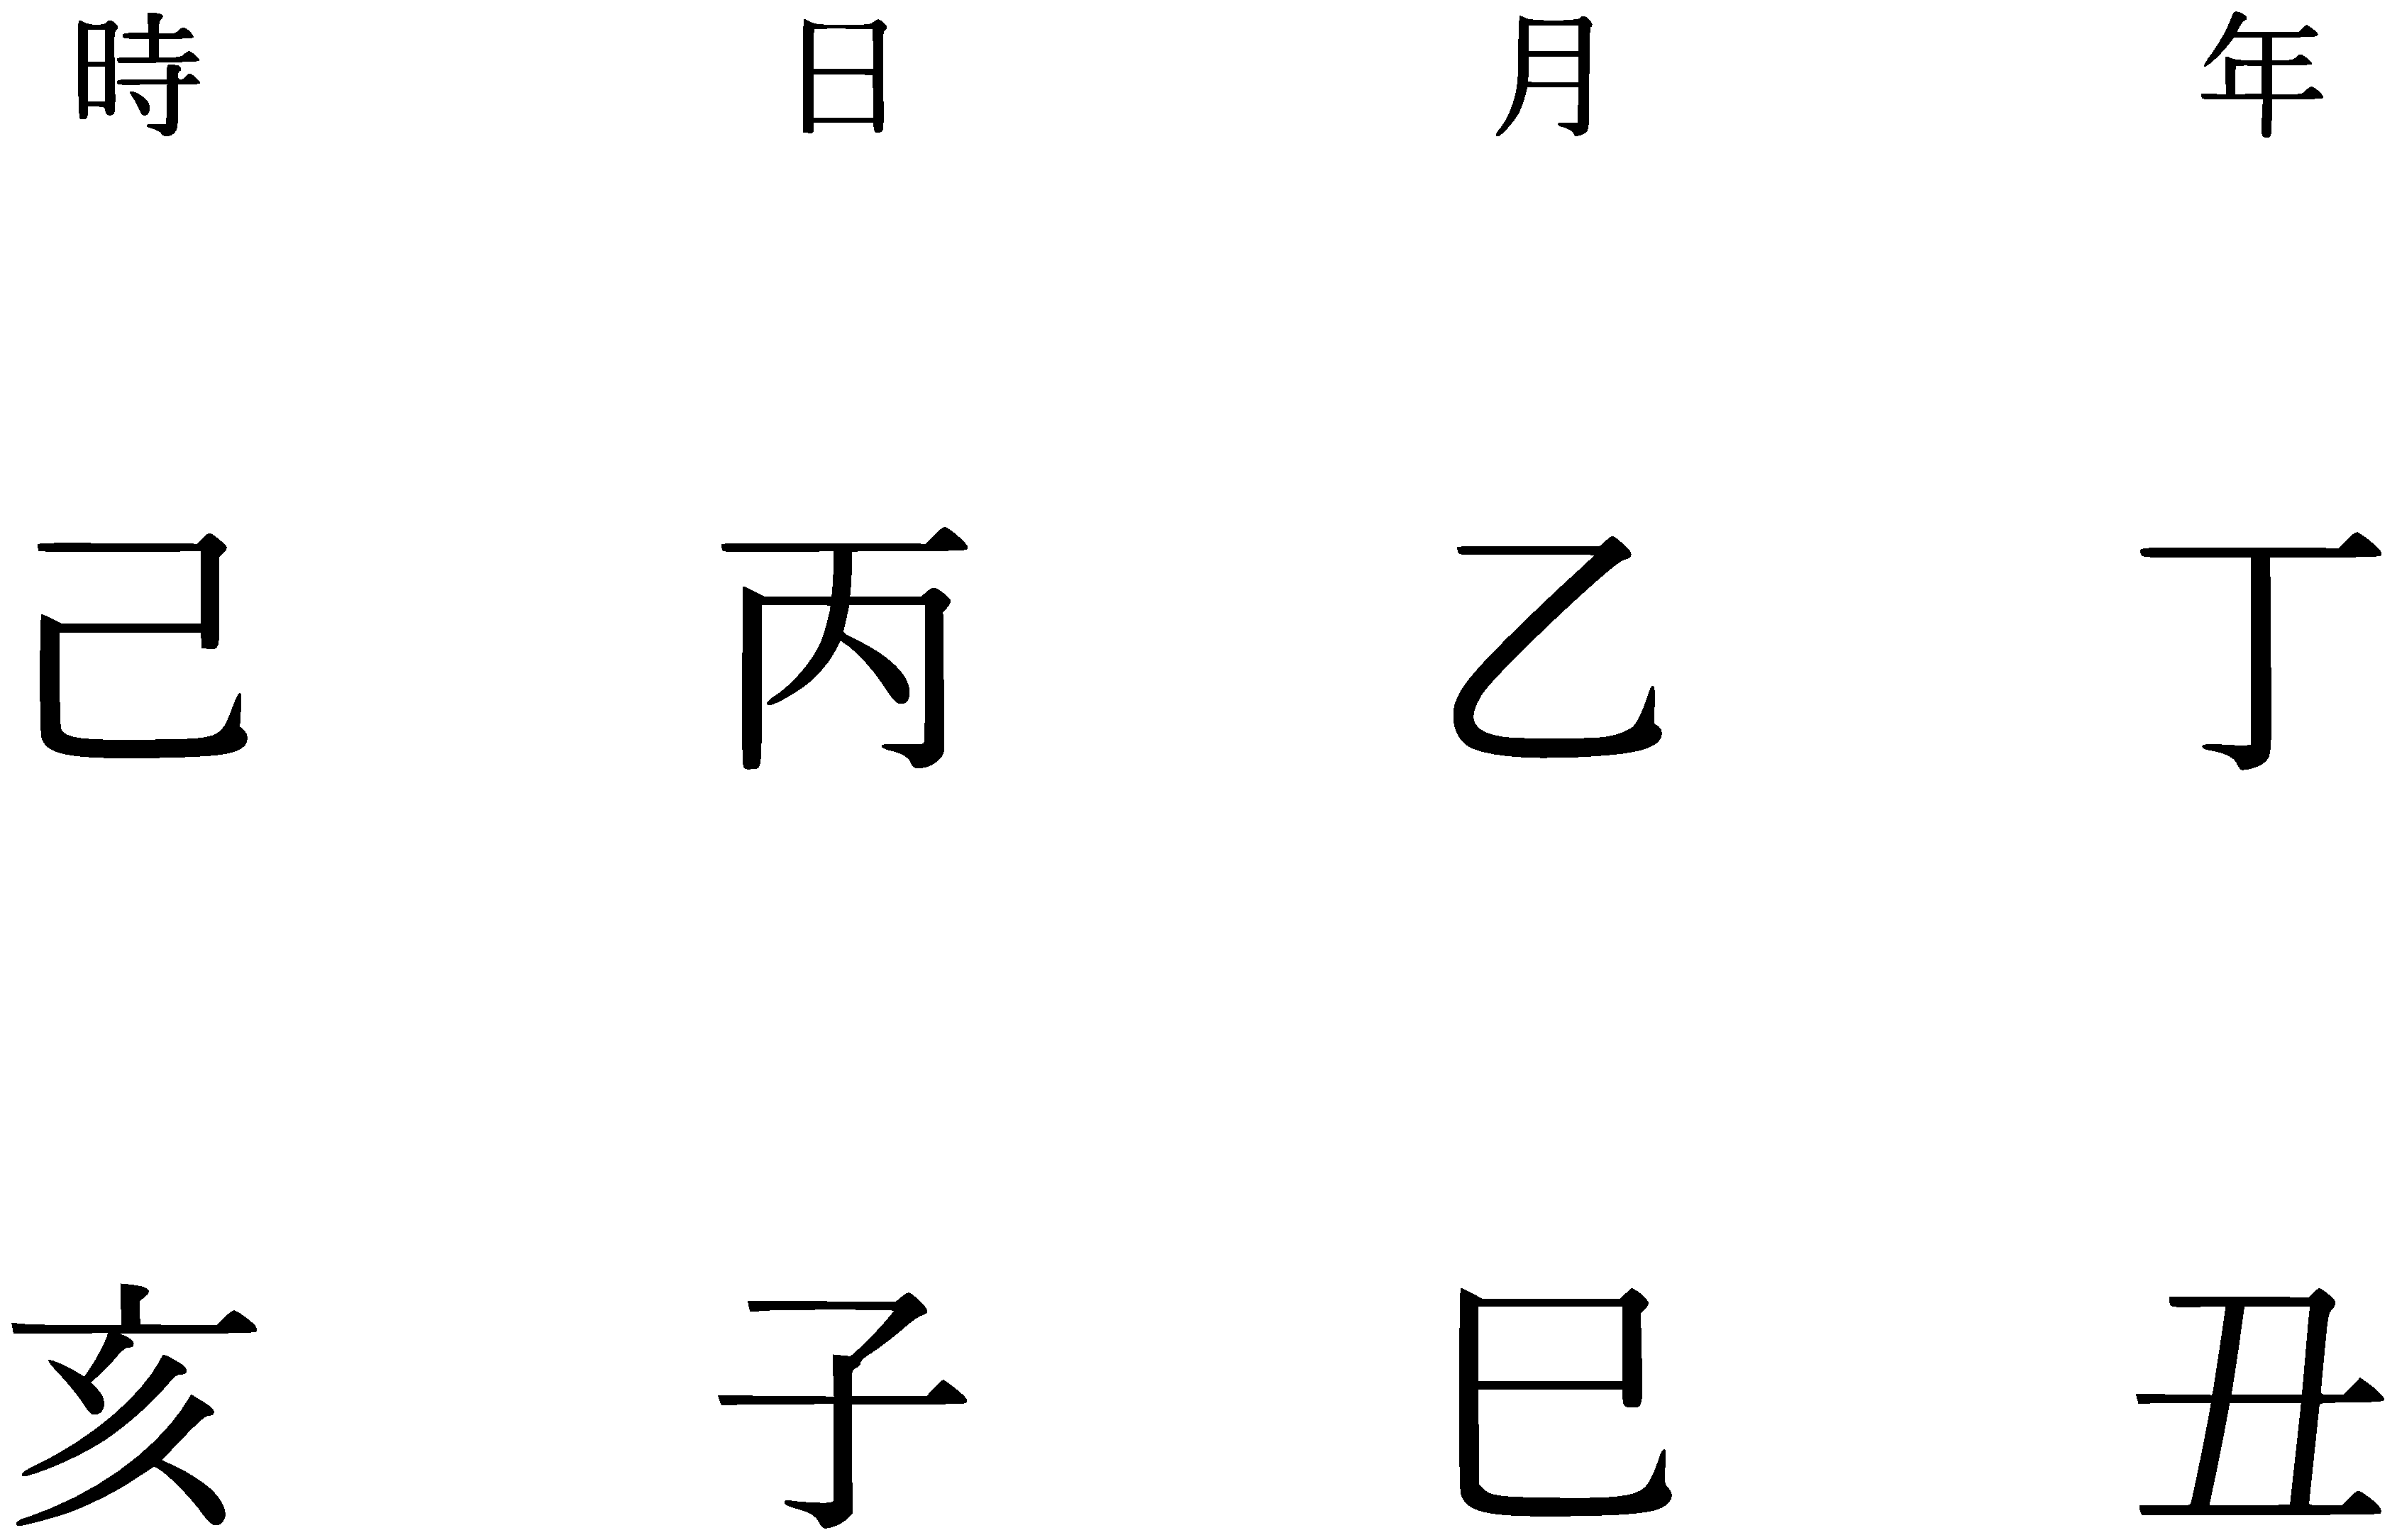
\includegraphics[width=45mm,angle=90]{figs/figure3-6.eps}
\end{figure}

\noindent
\\(4) 昭和\rensuji{57}年(1982年)1月4日2時\rensuji{23}分

まず、六十干支表から昭和\rensuji{57}+2=\rensuji{59}で年干支「壬戌」を得ます。しかし、1月はまだ節入りしていないため、前年の「辛酉」が年干支となります。次に、1月の標準節入日を参照すると「6日」であるため、1月4日はまだ節入りしていないことが分かります。そのため、月干支表の「辛」の行における「\rensuji{12}月子」を参照し、「庚」を得ます。月干支は「庚子」です。

生日基数表によれば、昭和\rensuji{57}年1月に対応する基数は「\rensuji{20}」ですので、\rensuji{20}+4=\rensuji{24}です。六十干支表において「\rensuji{24}」に対応する干支は「丁亥」ですので、これが日干支になります。最後に、時干支表の「丁」の行を参照すると、「1時より丑」は「辛」です。そのため、ここから時干支「辛丑」を得ます。

まとめると、昭和\rensuji{57}年1月4日2時\rensuji{23}分生まれの四柱干支は、次のとおりです。

\begin{figure}[h]
  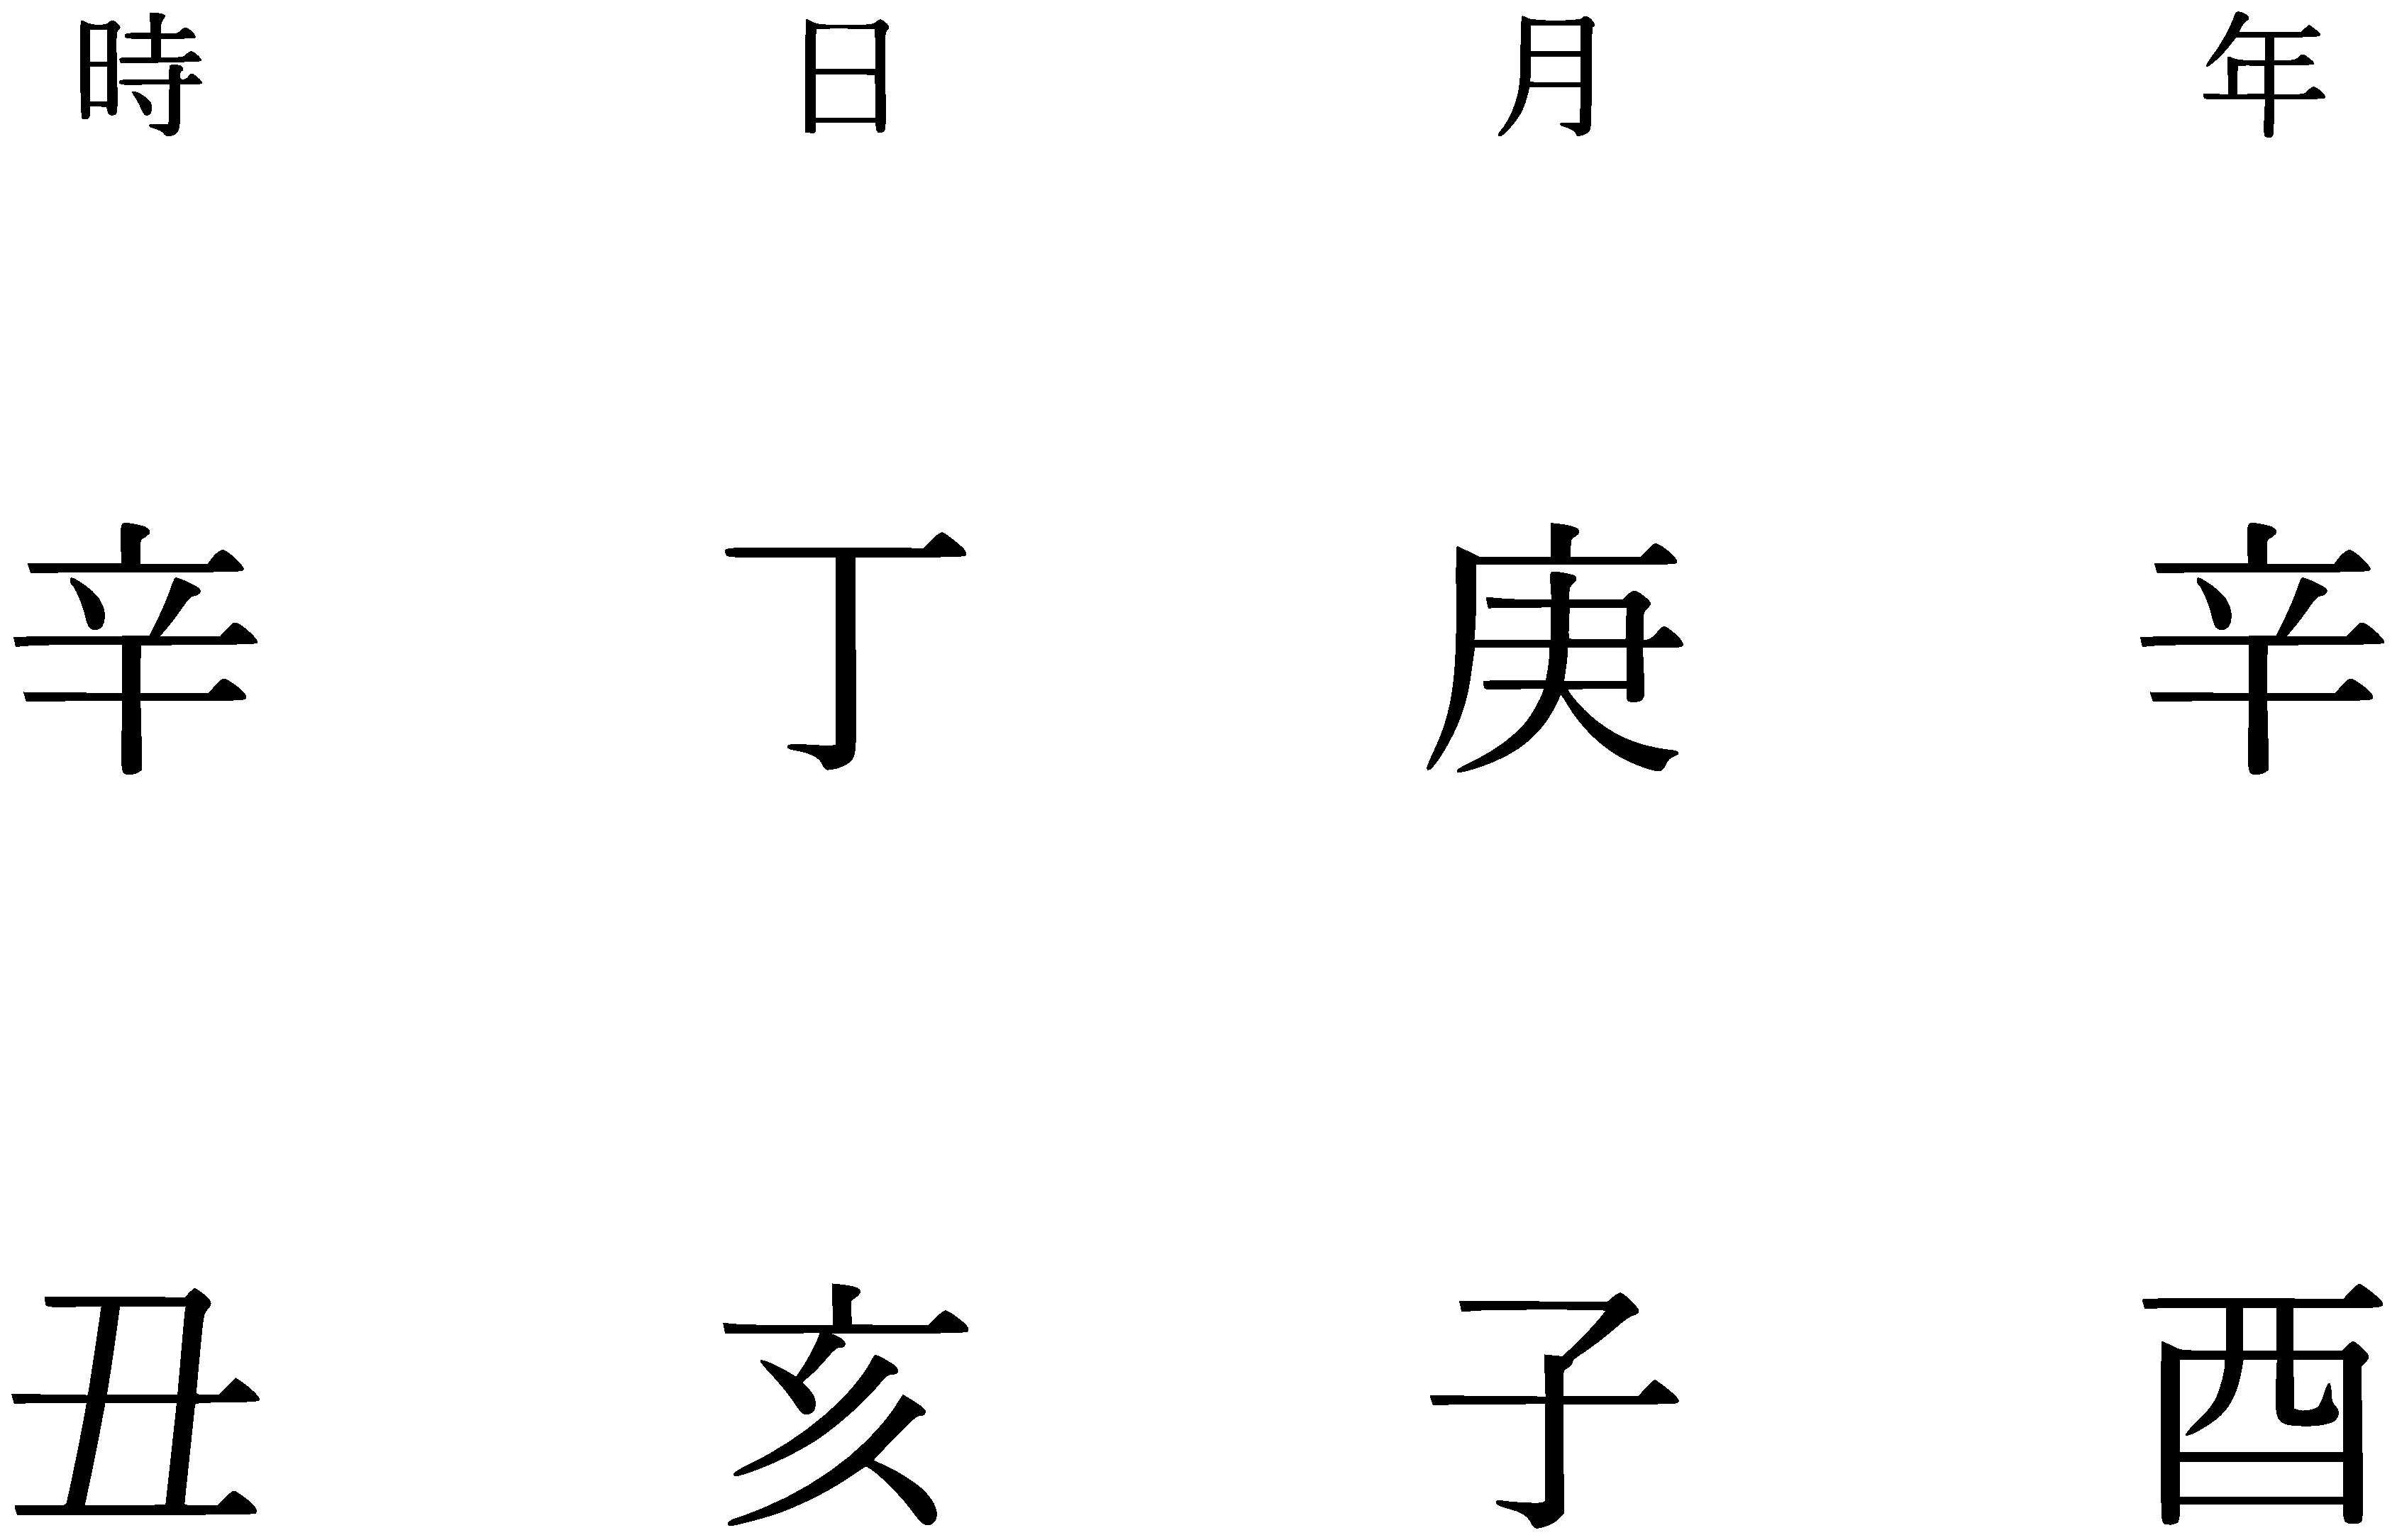
\includegraphics[width=45mm,angle=90]{figs/figure3-7.eps}
\end{figure}

\subsection{蔵干の導き方}
ここまでで、四柱干支(天干・地支)が求められるようになりました。ここから、次は「\ruby{蔵干}{ぞうかん}」を導きます。

蔵干は、月律(月のリズム)による運命の差異を表す干です。四柱推命学では、例えば、同じ平成\rensuji{10}年(1998年)\rensuji{11}月の「癸亥」月生まれでも、その月の前半(\ruby{初気}{しょき})に生まれるか、後半(\ruby{本気}{ほんき})に生まれるかで運命が異なり、その違いが地支に含まれていると考えます。

そこで、4つの支がそれぞれ蔵している干(蔵干)を導き出すことによって、その運命の差異を命式に反映させます。

蔵干は、次の蔵干表を用いて導きます。

\begin{figure}[h]
  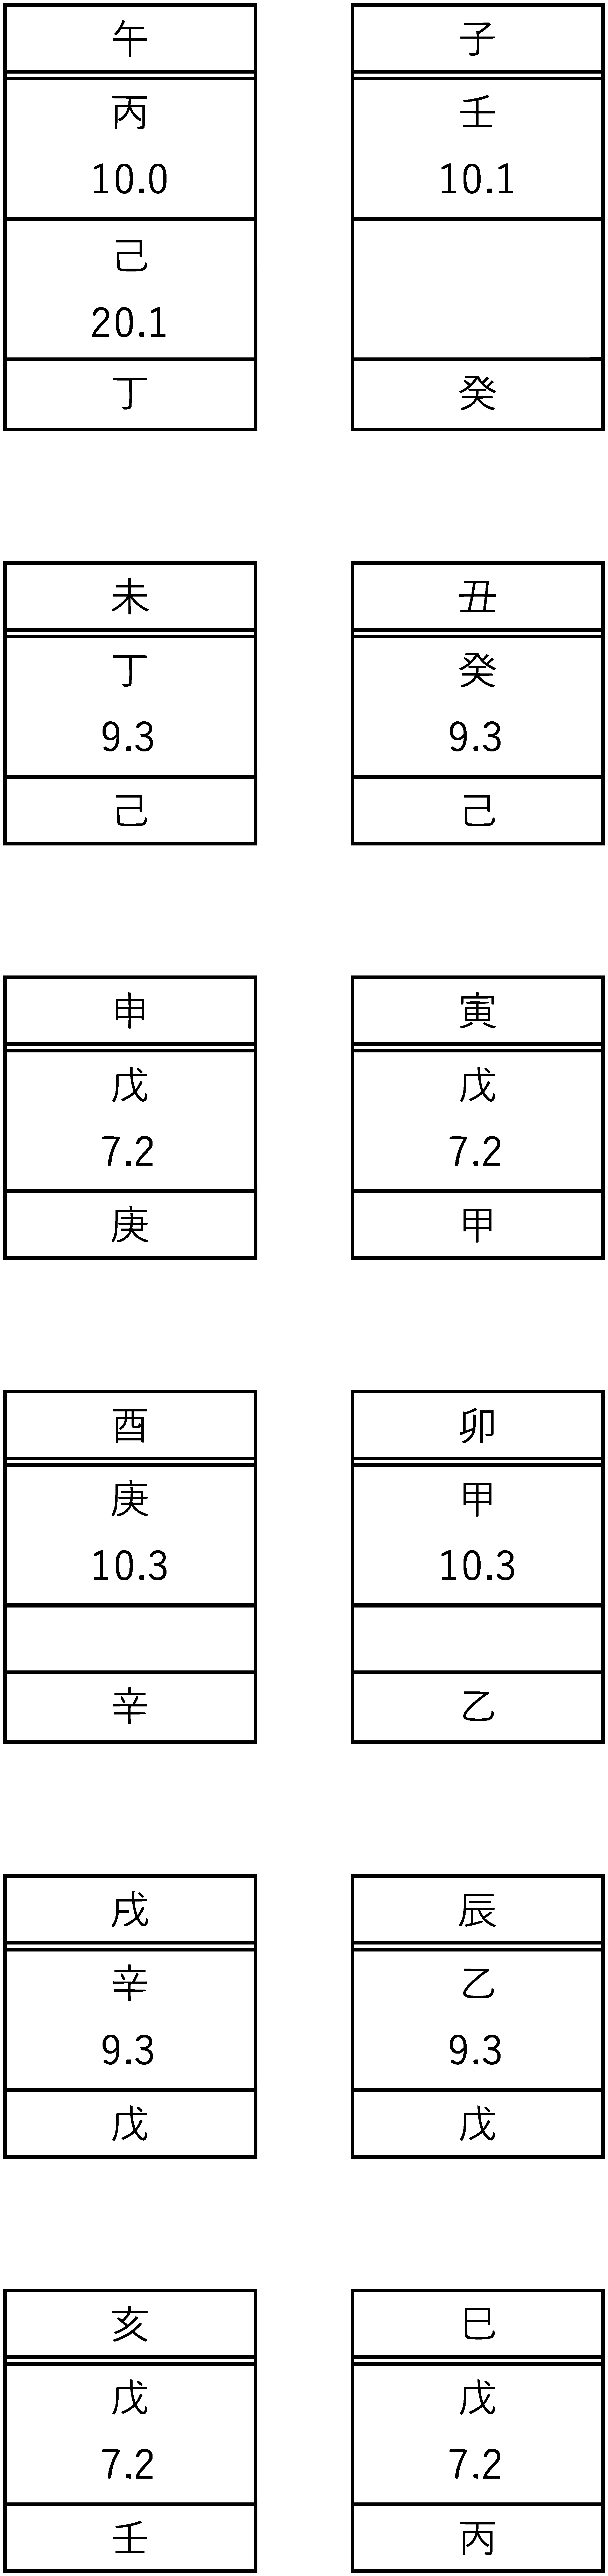
\includegraphics[width=30mm,angle=90]{figs/figure3-9.eps}
\end{figure}

平成3年(1991年)8月\rensuji{16}日9時\rensuji{30}分生まれの人の蔵干を導く例を説明します。

まず、年支は「未」ですので、蔵干表の「未」欄を参照すると、「丁\rensuji{9.3}」と「己」と書かれています。この「\rensuji{9.3}」は節入りからの経過日時を表します。つまり、節入りから誕生日時までの経過日時が9日と3時間までであれば、「丁」を蔵干とし、それ以降であれば「己」を蔵干とすることを意味します。

月干支表によれば、8月の標準節入日は8日ですので、8月\rensuji{16}日9時\rensuji{30}分は、節入りからだいたい8日と9時間\rensuji{30}分です。これは「9日と3時間まで」に該当するため、年支蔵干は「丁」になります。

次に、月支は「申」ですので、蔵干表の「申」欄を参照すると、「戊\rensuji{7.2}」と「庚」と書かれています。8日と9時間\rensuji{30}分は「7日と2時間以降」に該当するため、月支蔵干は「庚」になります。

さらに、日支は「午」ですので、蔵干表の「午」欄を参照すると、「丙\rensuji{10.0}」、「己\rensuji{20.1}」、「丁」と書かれています。8日と9時間\rensuji{30}分は「\rensuji{10}日と0時間まで」に該当するため、日支蔵干は「丙」になります。

最後に、時支は「巳」ですので、蔵干表の「巳」欄を参照すると、「戊\rensuji{7.2}」と「丙」と書かれています。8日と9時間\rensuji{30}分は「7日と2時間以降」に該当するため、時支蔵干は「丙」になります。

\begin{figure}[h]
  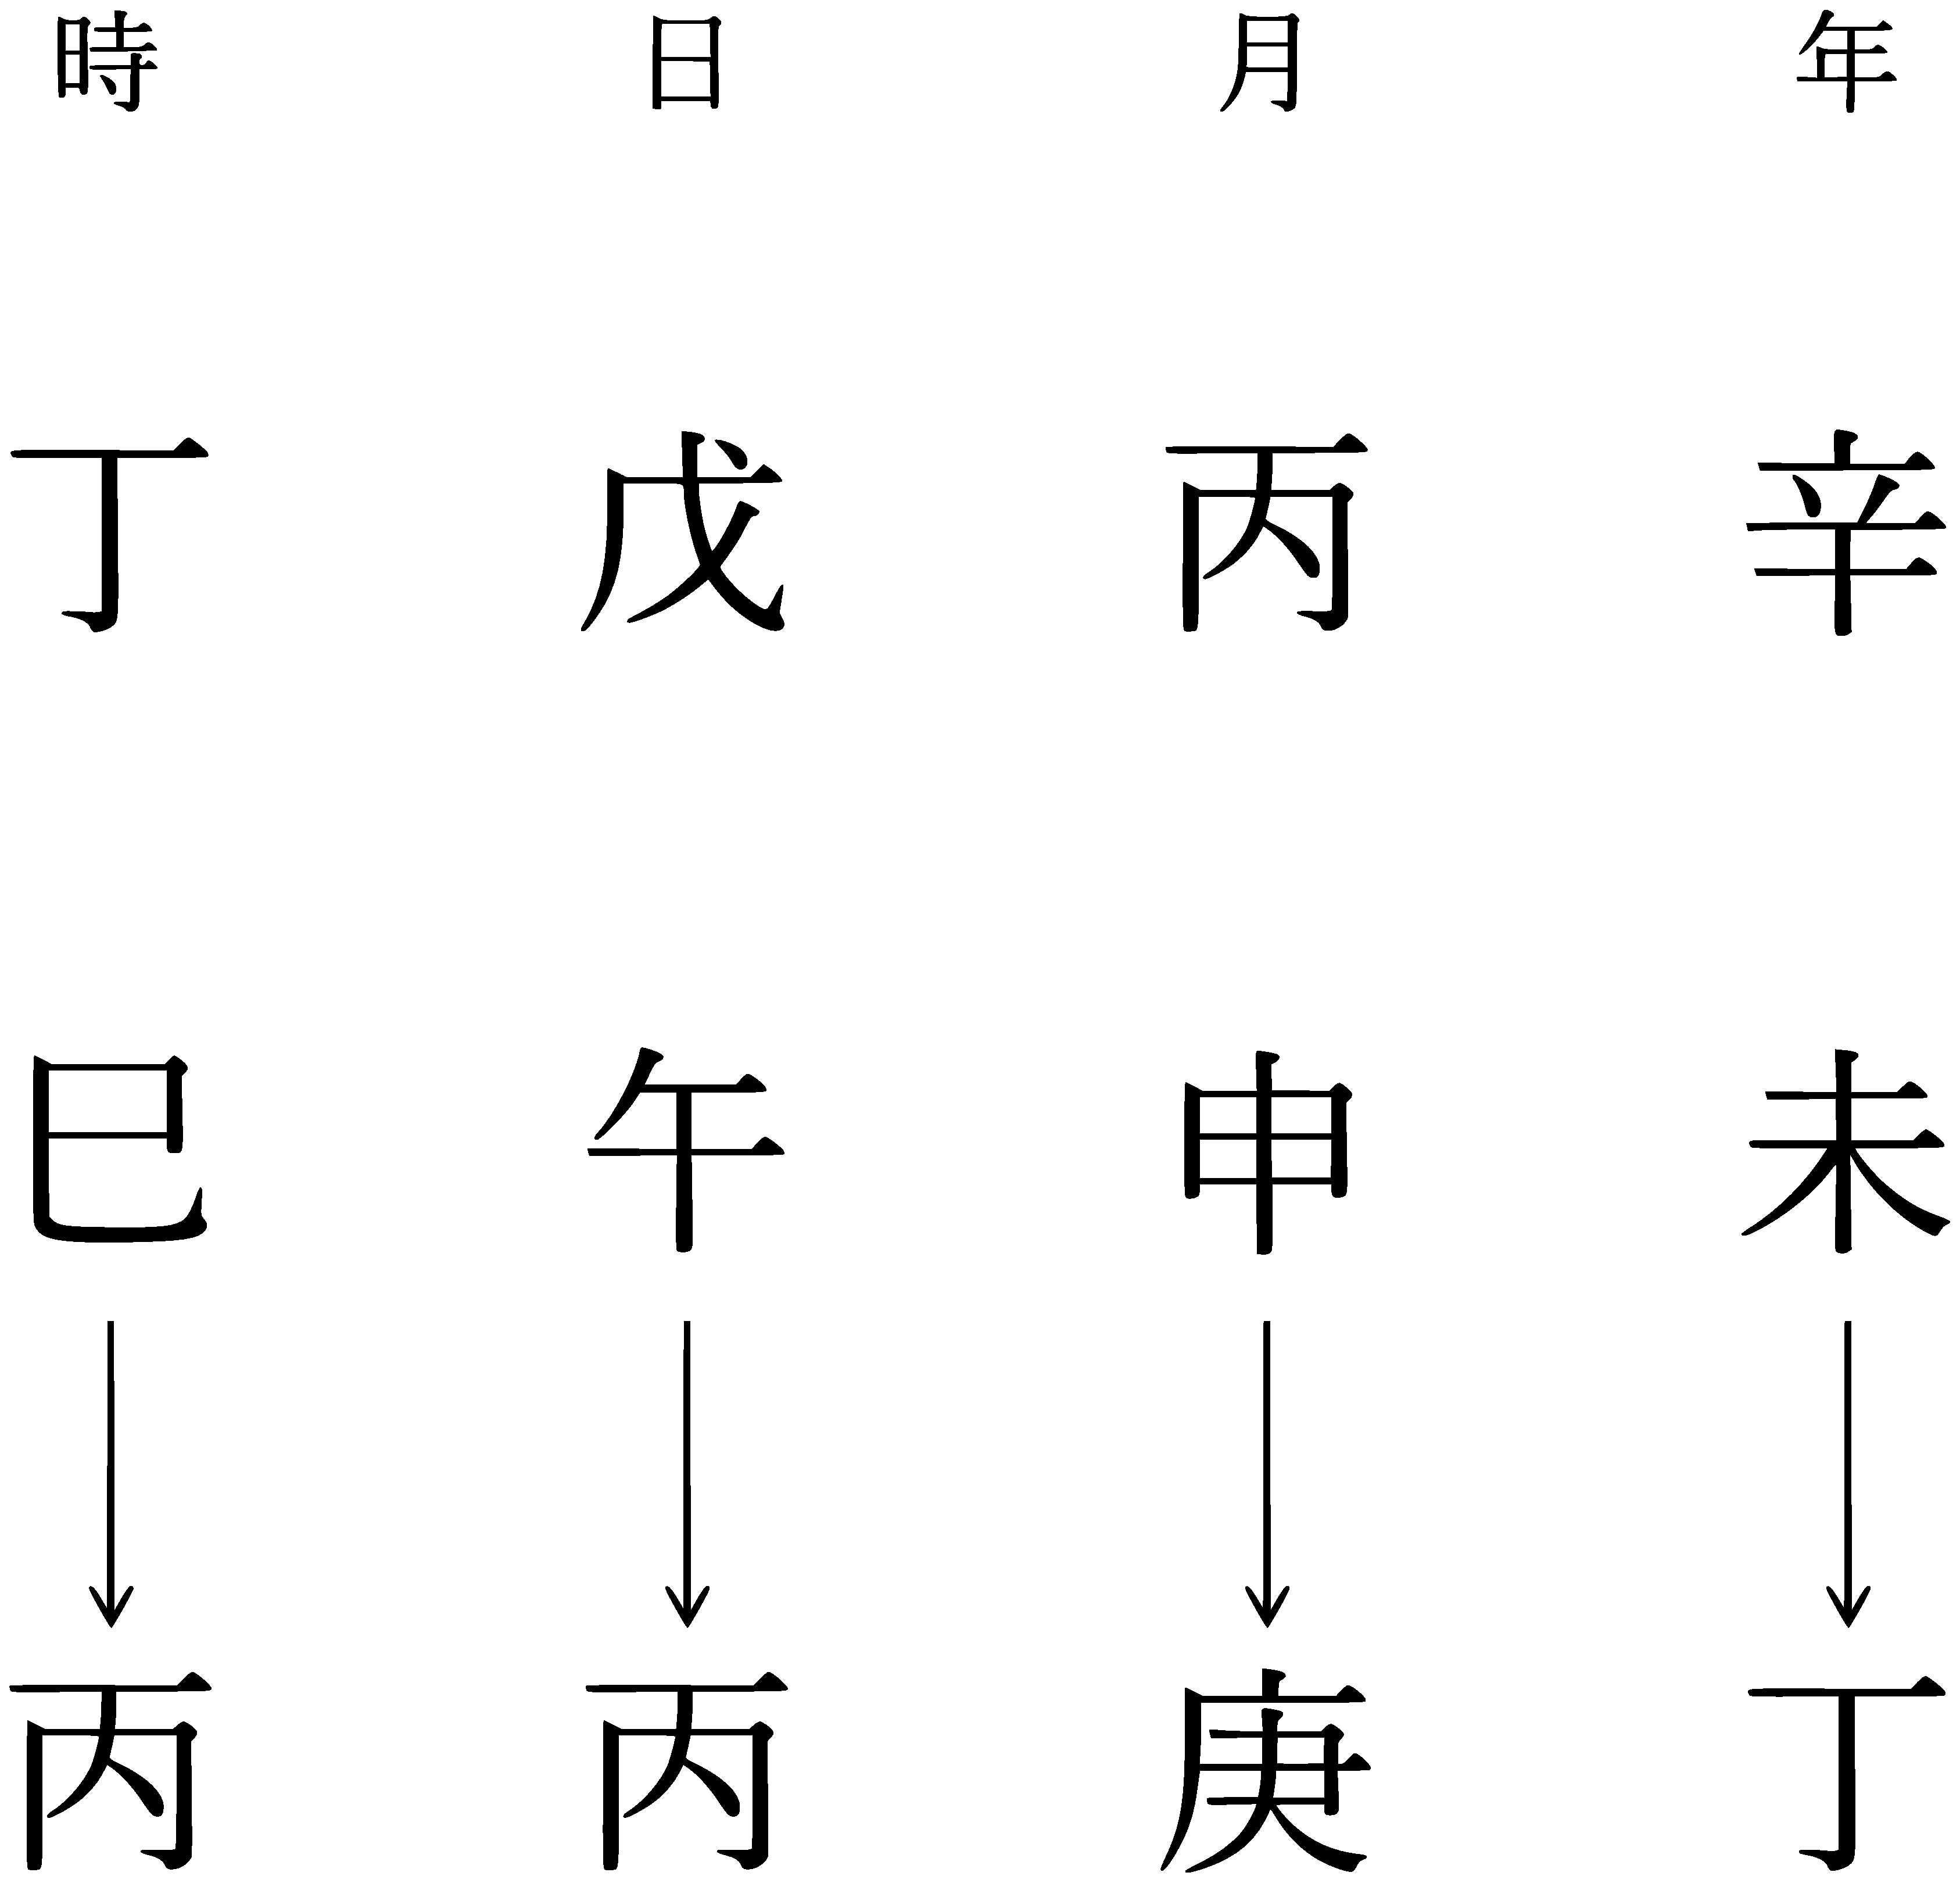
\includegraphics[width=45mm,angle=90]{figs/figure3-10.eps}
\end{figure}

ここで、「午」の蔵干のみ変則的であることに注意しましよう。つまり、蔵干表に記載のとおり、節入りから誕生日時までの経過日時が、\rensuji{10}日と0時間までであれば「丙」、\rensuji{10}日と0時間以降かつ\rensuji{20}日と1時間までであれば「己」、\rensuji{20}日と1時間以降であれば「丁」を蔵干とします。 \footnote{午のみ蔵干が変則的となる詳しい理屈は、ここでは割愛します。}\\

次に、平成2年(1990年)9月\rensuji{25}日8時\rensuji{41}分生まれの人の蔵干を導く例を説明します。

まず、月干支表によれば、9月の標準節入日は8日ですので、9月\rensuji{25}日8時\rensuji{41}分は、節入りからだいたい\rensuji{13}日と8時間\rensuji{41}分です。年支は「午」ですので、蔵干表の「午」欄を参照すると、「丙\rensuji{10.0}」、「己\rensuji{20.1}」、「丁」と書かれています。\rensuji{13}日と8時間\rensuji{41}分は「\rensuji{10}日と0時間以降かつ\rensuji{20}日と1時間まで」に該当するため、年支蔵干は「己」になります。

次に、月支は「酉」ですので、蔵干表の「酉」欄を参照すると、「庚\rensuji{10.3}」と「辛」と書かれています。\rensuji{13}日と8時間\rensuji{41}分は「\rensuji{10}日と3時間以降」に該当するため、月支蔵干は「辛」になります。

さらに、日支は「巳」ですので、蔵干表の「巳」欄を参照すると、「戊\rensuji{7.2}」、「丙」と書かれています。\rensuji{13}日と8時間\rensuji{41}分は「7日と2時間まで」に該当するため、日支蔵干は「丙」になります。

最後に、時支は「辰」ですので、蔵干表の「辰」欄を参照すると、「乙\rensuji{9.3}」と「戊」と書かれています。\rensuji{13}日と8時間\rensuji{41}分は「9日と3時間以降」に該当するため、時支蔵干は「戊」になります。

\begin{figure}[h]
  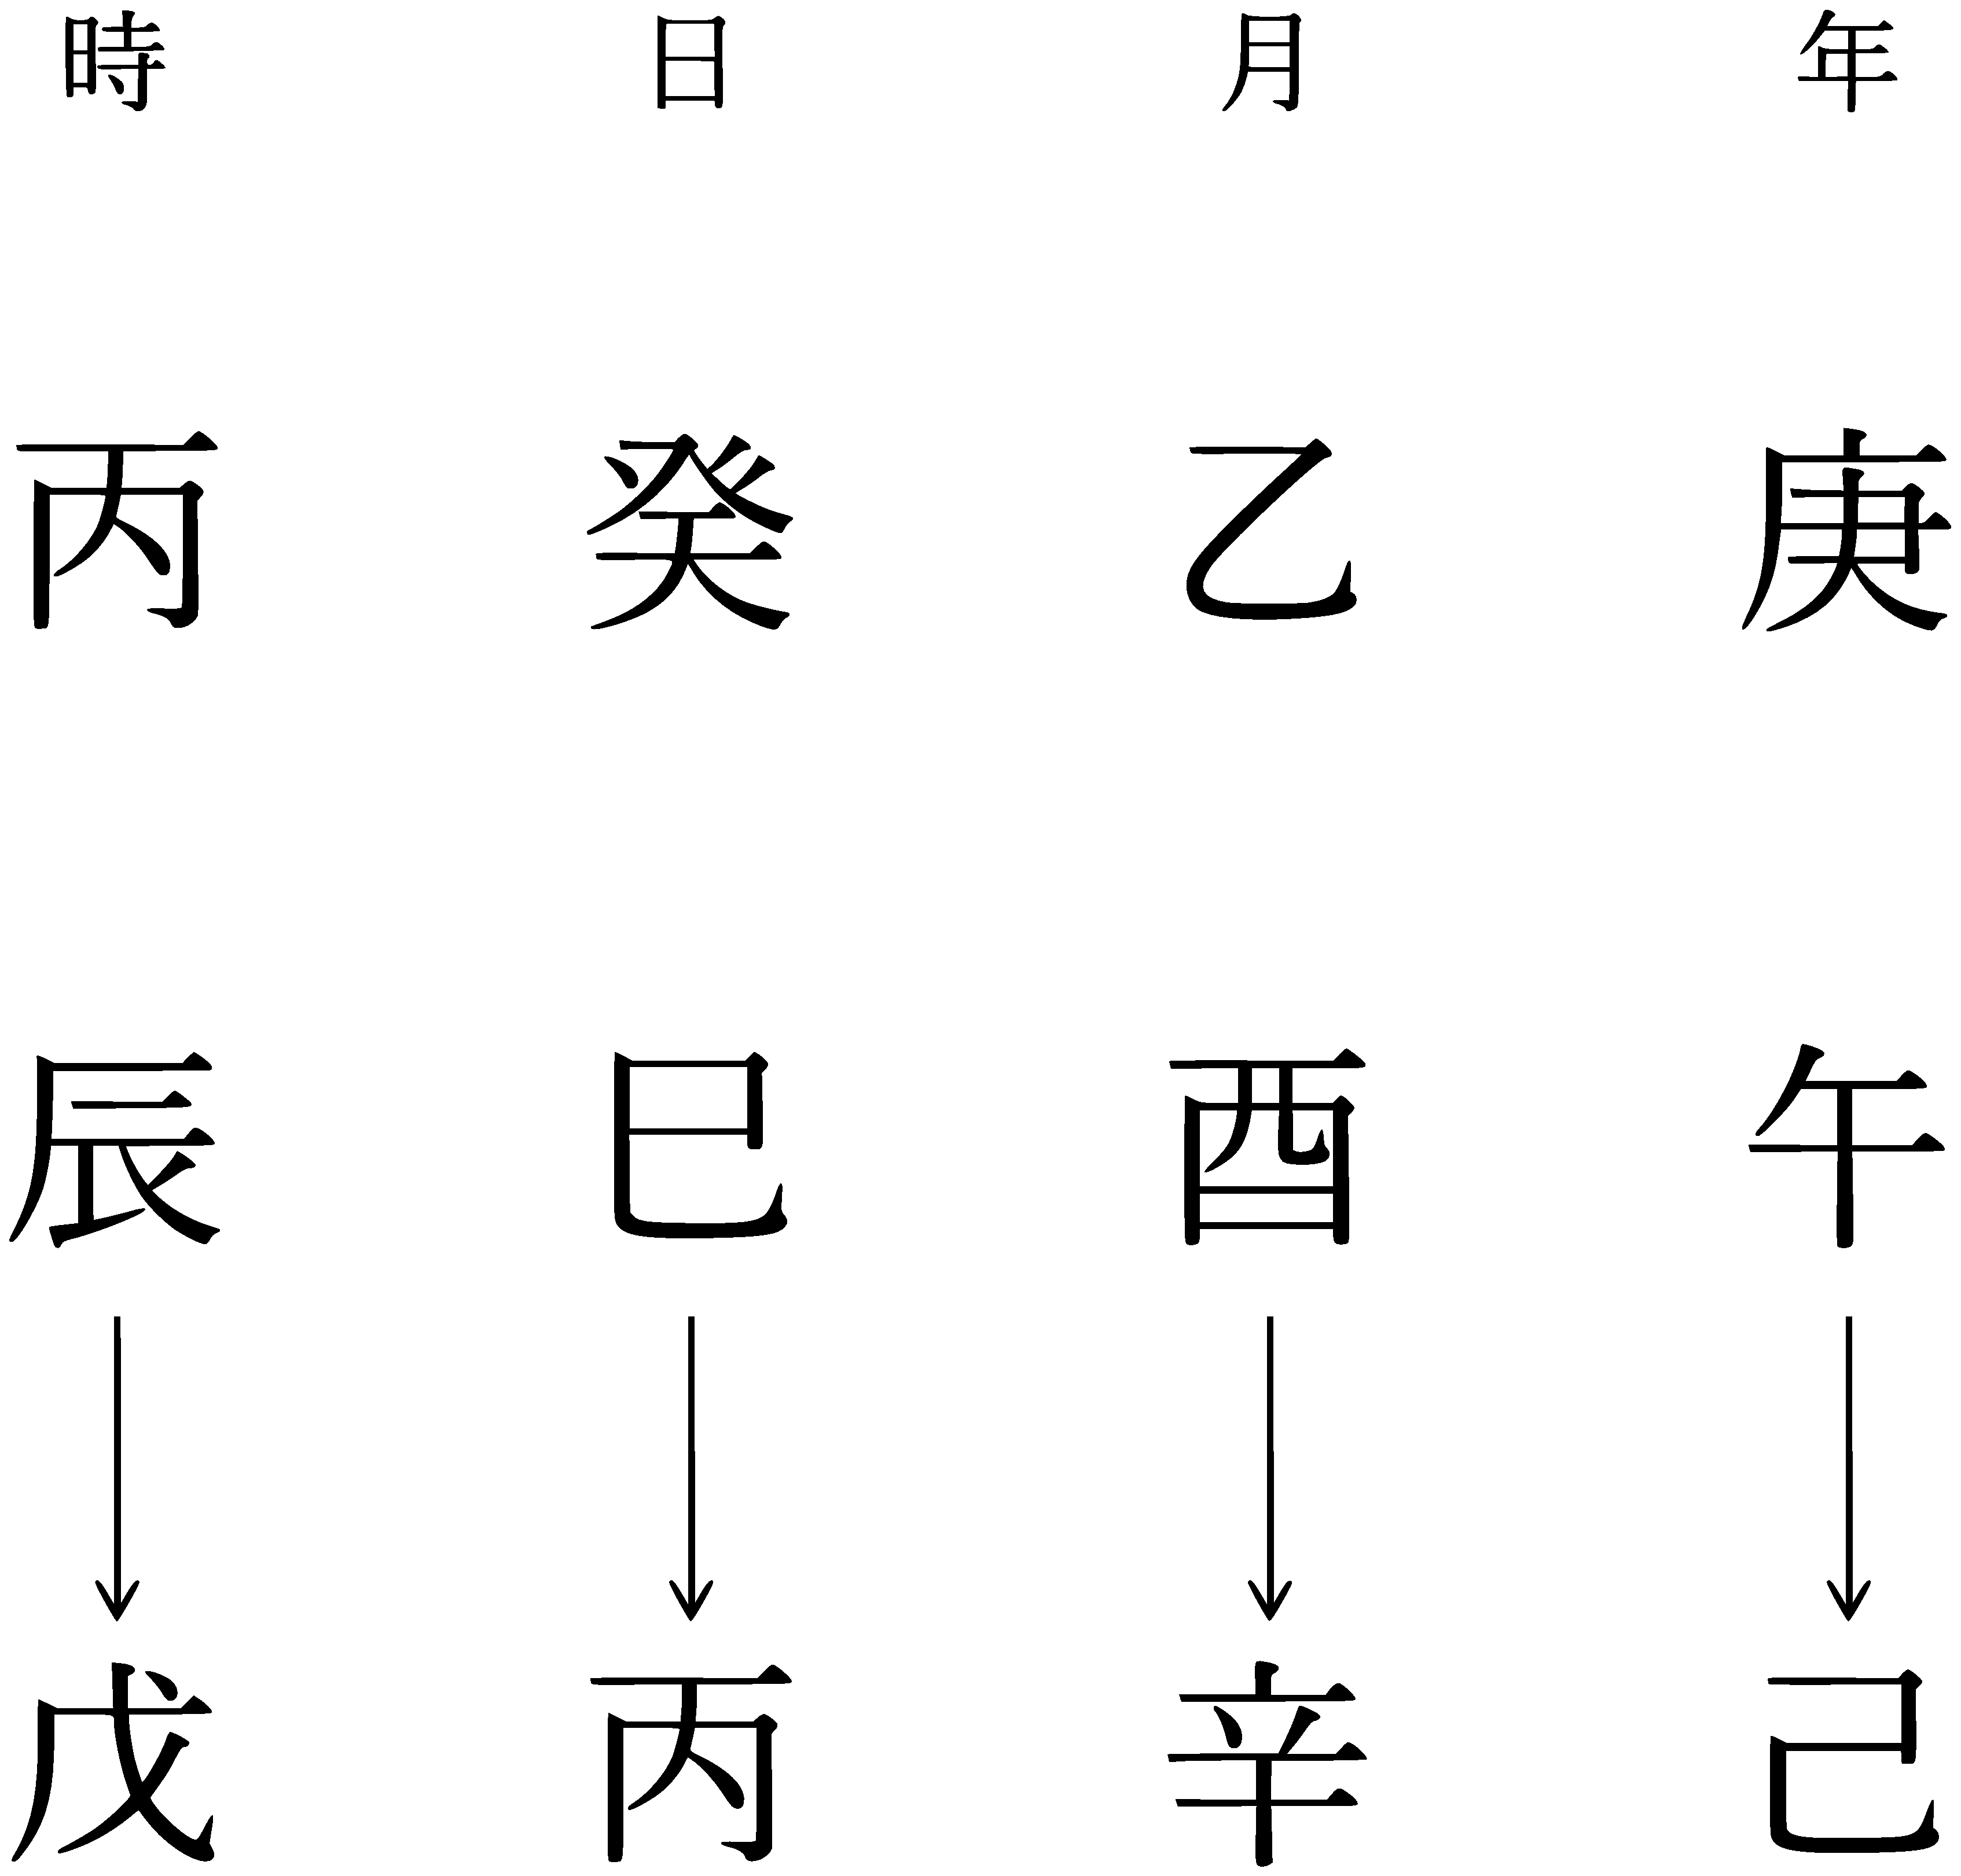
\includegraphics[width=45mm,angle=90]{figs/figure3-11.eps}
\end{figure}

\subsection{命式の求め方のまとめ}
四柱干支(天干・地支)を求めて蔵干を導くと、命式が完成します。これで、その人が持って生まれた運命を推測する準備が整いました。その方法は後で詳しく説明するとして、最後に命式の求め方をまとめます。

\begin{enumerate}
  \item 年干支を求める
  \begin{enumerate}
  \item 昭和であれば2を足し、平成であれば5を足し、令和であれば\rensuji{35}を足す(足した数が\rensuji{60}を超過している場合は\rensuji{60}を引く)
  \item 足した数に対応する干支を六十干支表から得る\\
    ※節入りの有無に注意すること
  \end{enumerate}
\item 月干支を求める
  \begin{enumerate}
  \item 年柱天干に対応する干支を月干支表から得る\\
    ※節入りの有無に注意すること
  \end{enumerate}
  \item 日干支を求める
    \begin{enumerate}
    \item 生日基数表から年月に対応する基数を得る
    \item その基数に日の数を足す(足した数が\rensuji{60}を超過している場合は\rensuji{60}を引く)
    \item 足した数に対応する干支を六十干支表から得る
    \end{enumerate}
  \item 時干支を求める
    \begin{enumerate}
    \item 日干に対応する干支を時干支表から得る
    \end{enumerate}
  \item 蔵干を導く
    \begin{enumerate}
    \item 節入りから誕生日時までの経過日時と蔵干表に基づいて、各支が蔵する干を導く
    \end{enumerate}
  \end{enumerate}

命式の求め方は機械的です。四柱推命学を志す人は、まずこれを求める方法に習熟する必要がありますので、何度も練習しましょう。

\subsection{五行配分}
四柱干支が出揃えば、五行の配分が明らかになります。例えば、平成元年\rensuji{11}月\rensuji{26}日\rensuji{13}時\rensuji{45}分生まれの四柱干支は、次のとおりであり、五行配分は、木2、火1、土2、金1、水2であることが分かります。\footnote{十干十二支と五行との関係は、第2章を参照。}

\begin{figure}[h]
  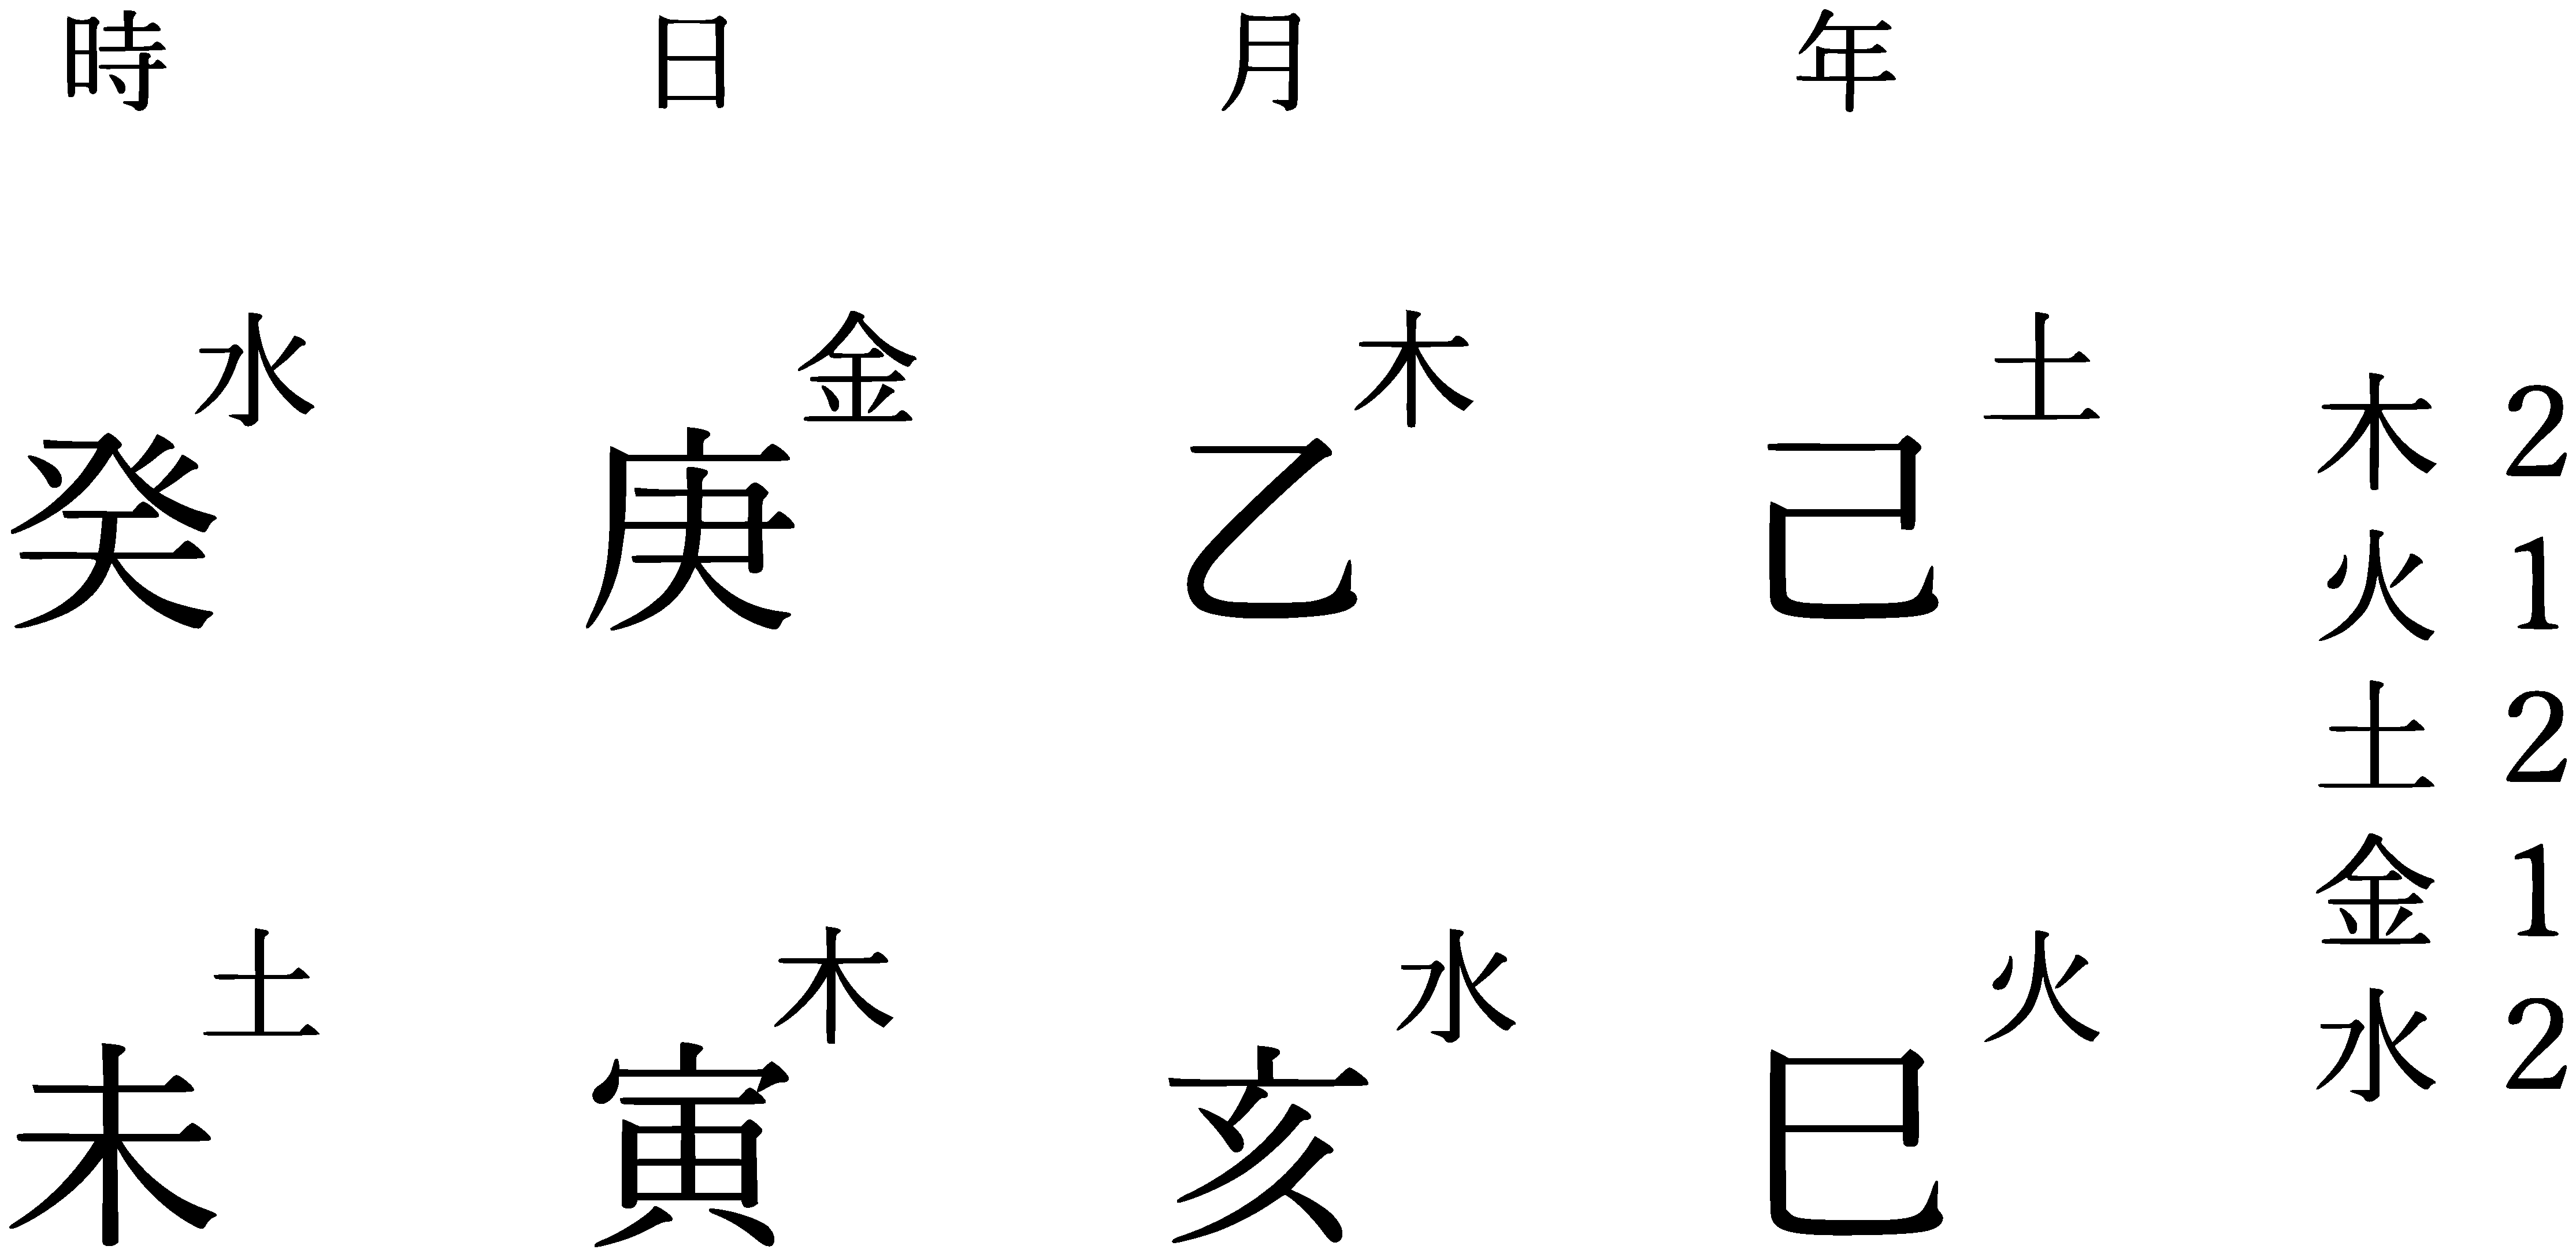
\includegraphics[width=55mm,angle=90]{figs/figure3-12.eps}
\end{figure}

五行配分は、命式を解釈する上で重要な情報になります。例えば、右の例のように、四柱干支に木火土金水の五行がすべて揃っている場合、その性格は穏やかな傾向があり、人生に多少の動揺があってもその衝撃を吸収できるため、浮き沈みの緩やかな生涯を送れると一応解釈されます。

なお、このように五行が揃っていることを「\ruby{五行周流}{ごぎょうしゅうりゅう}」と呼びます。中庸と均衡を重視する四柱推命学では、この状態を大変喜びます。\footnote{全人口の約\rensuji{15}パーセントの人が五行周流に恵まれているといわれます。}

逆に、木火金水が3つ以上配分されている場合、または、土が4つ以上配分されている場合、その五行は「多い」と判断され、なんらかの偏りがあると分かります。

\subsection{空亡(天中殺)}
六十干支表のように、十干と十二支を組み合わせていくと、支が二つ余ります。この干のない支を\ruby{空亡}{くうぼう}(\ruby{天中殺}{てんちゅうさつ})といいます。「\ruby{空}{むな}しく\ruby{亡}{ほろ}びる」の字義どおり、空亡が現れた柱はその働きが弱まります。

空亡は、六十干支表の最下段に記載されており、日干支から求められます。例えば、先の例では、日干支は「\rensuji{27}庚寅」であるため、その列の六十干支表の最下段を参照すると、「午未」が空亡であることが分かります。

\begin{figure}[h]
  \centering
  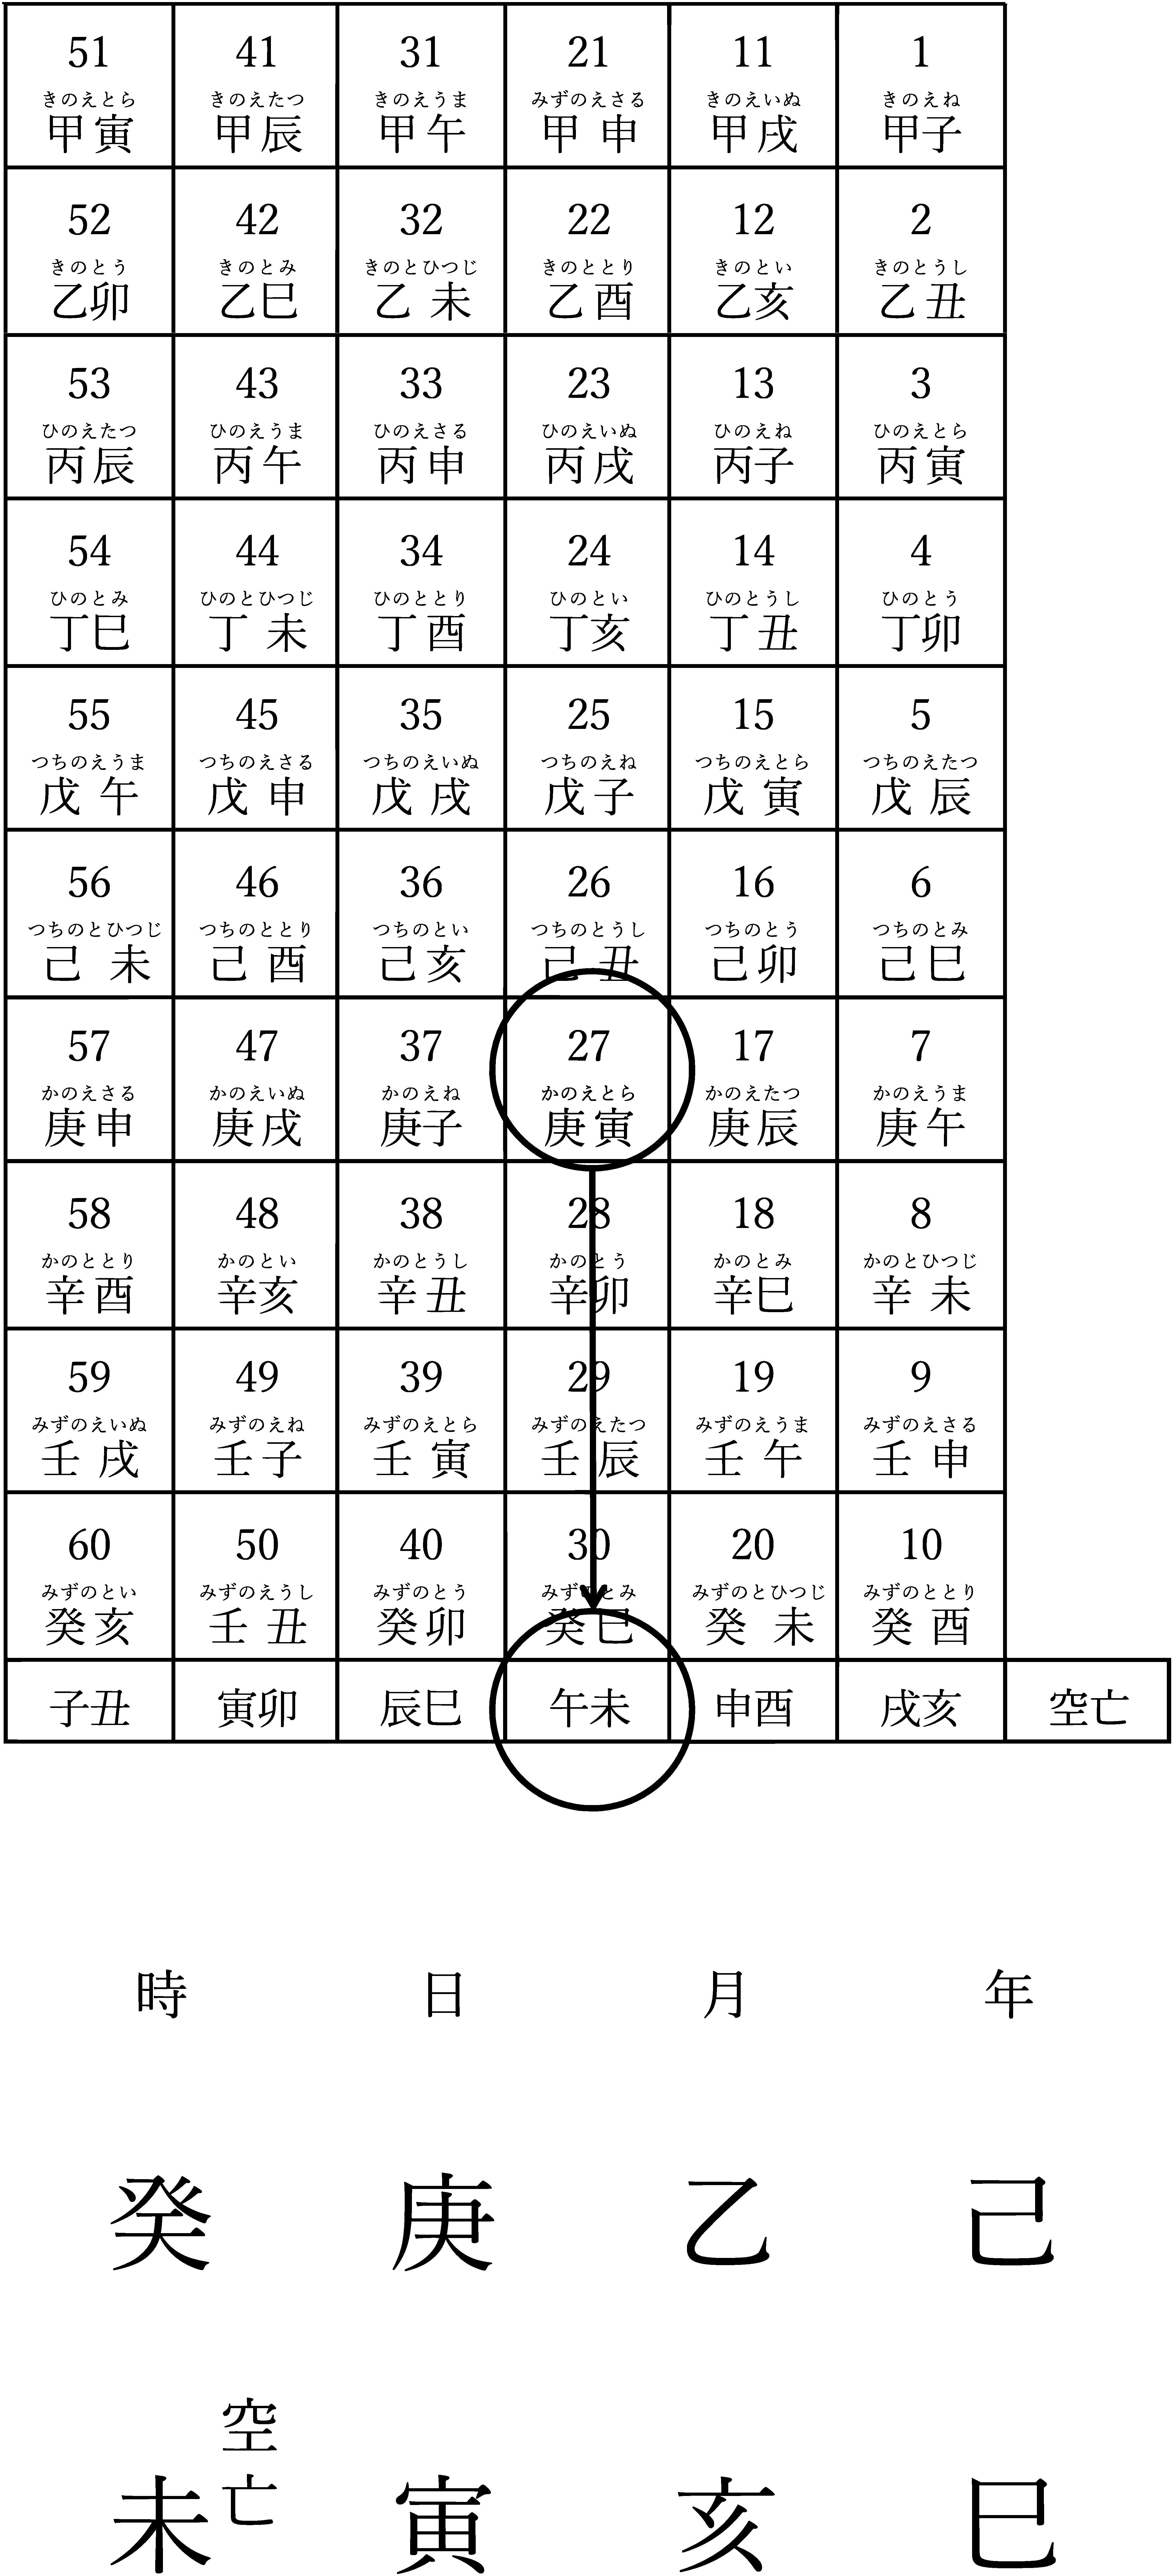
\includegraphics[width=60mm,angle=90]{figs/figure3-13.eps}
\end{figure}

先の四柱干支を再度確認すると、時支に「未」があるため、時柱が空亡していることが分かります。

命式に空亡が現れた場合の看命方法については、後の章で詳しく説明します。ここでは「時柱は空しく亡びているため、その働きが弱まる」と覚えておきましょう。

\subsection{調候}
\ruby{調候}{ちょうこう}とは、日干の季節バランスのことです。



\subsection{まとめ}


\clearpage

\section{大運}

\ruby{大運}{だいうん}は、一〇年ごとの運気の流れ(後天運勢)を干支で表現したものです。月柱の干支が大運の出発点となり、以後は立運年数から一〇年ごとに、六十干支表にしたがって大運の干支が変わっていきます。

ここで、大運が六十干支表にしたがって順に進んでいくのを「\ruby{順運}{じゅんうん}」といいます。逆に、六十干支表を遡って進んでいくのを「\ruby{逆運}{ぎゃくうん}」といいます。\footnote{順運・逆運に良し悪しはありません。つまり、順運であるから運勢が良いとか、逆運であるから運勢が悪いとかという意味はありません。}

例えば、月柱干支が「己丑」の順運であった場合、大運は「庚寅」「辛卯」「壬辰」「癸巳」…の順に進んでいきます。逆に、逆運であった場合、大運は「戊子」「丁亥」「丙戌」「乙酉」…の順に遡っていきます。

\begin{figure}[h]
  \centering
  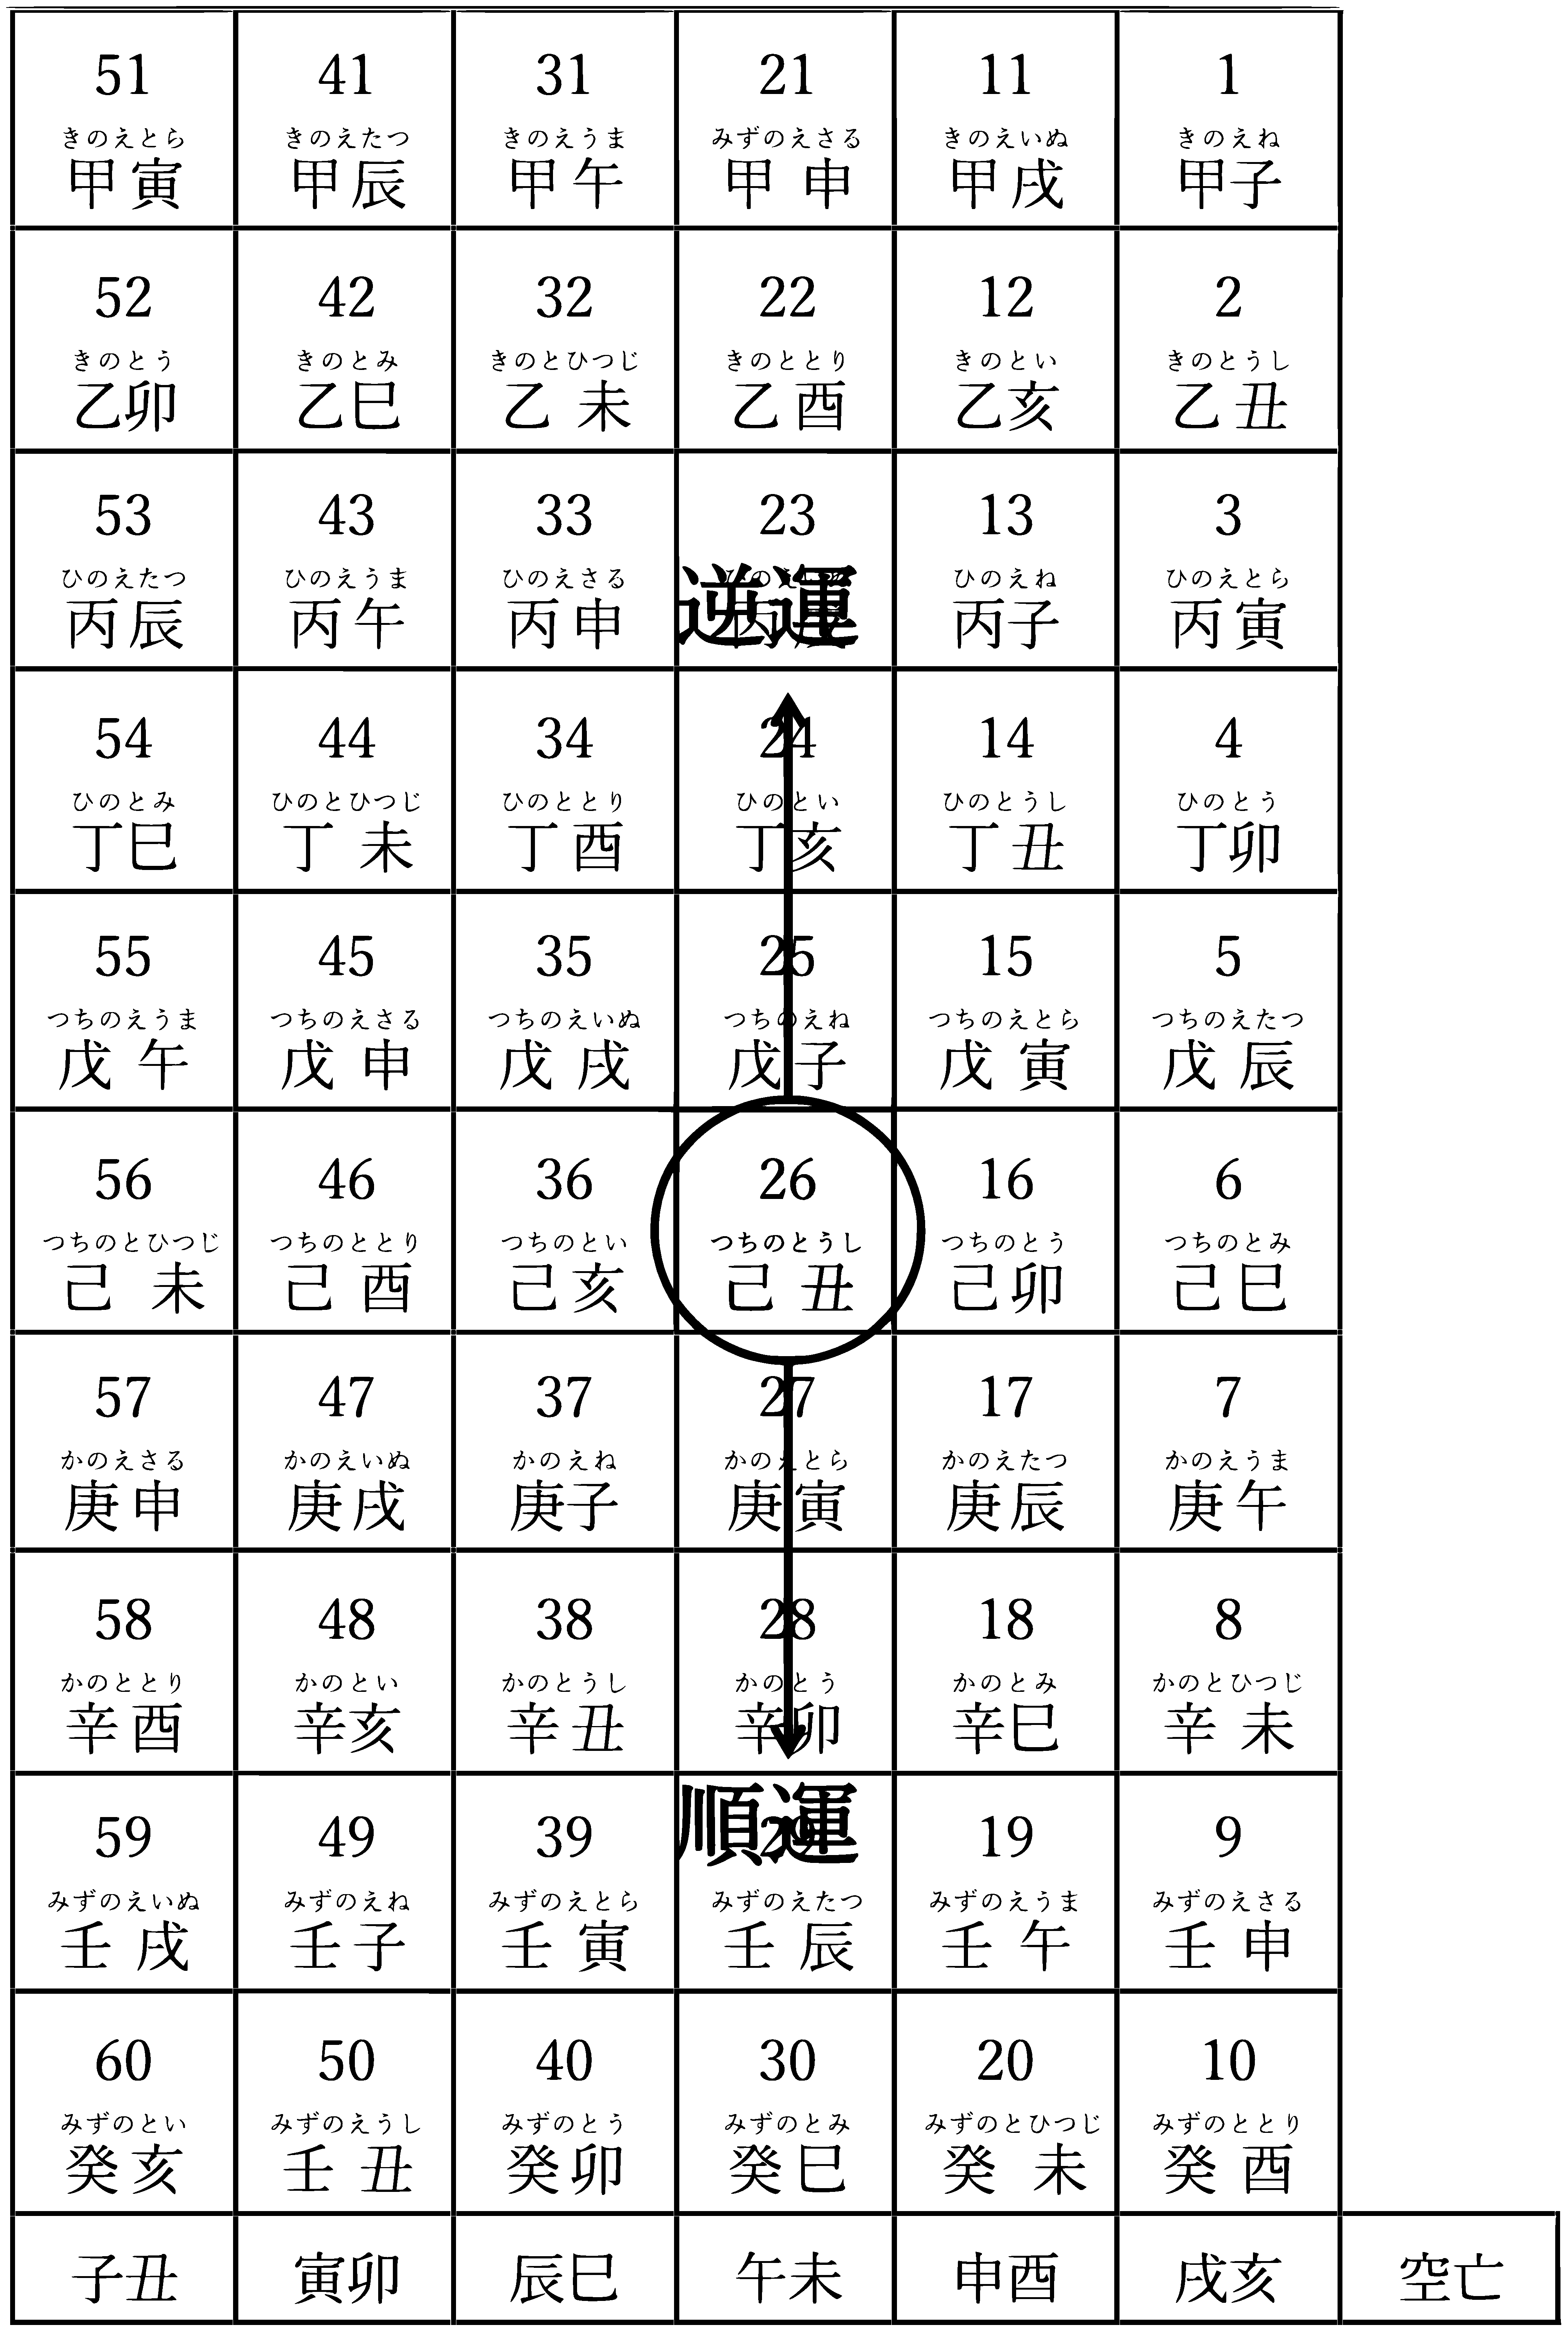
\includegraphics[width=75mm,angle=90]{figs/figure4-1.eps}
\end{figure}

\subsection{大運の求め方}
\subsubsection*{順運と逆運の決定と干支の配置}
大運を求めるためには、まず、その人の運勢が順運か逆運かを決定しなければなりません。これには性別と年柱天干を利用します。

(1)	男性…年柱天干が「陽干」の場合 → 順運\\
        年柱天干が「陰干」の場合 → 逆運

(2)	女性…年柱天干が「陽干」の場合 → 逆運\\
        年柱天干が「陰干」の場合 → 順運\\

次の命式を例に用いて説明します。

\begin{figure}[h]
  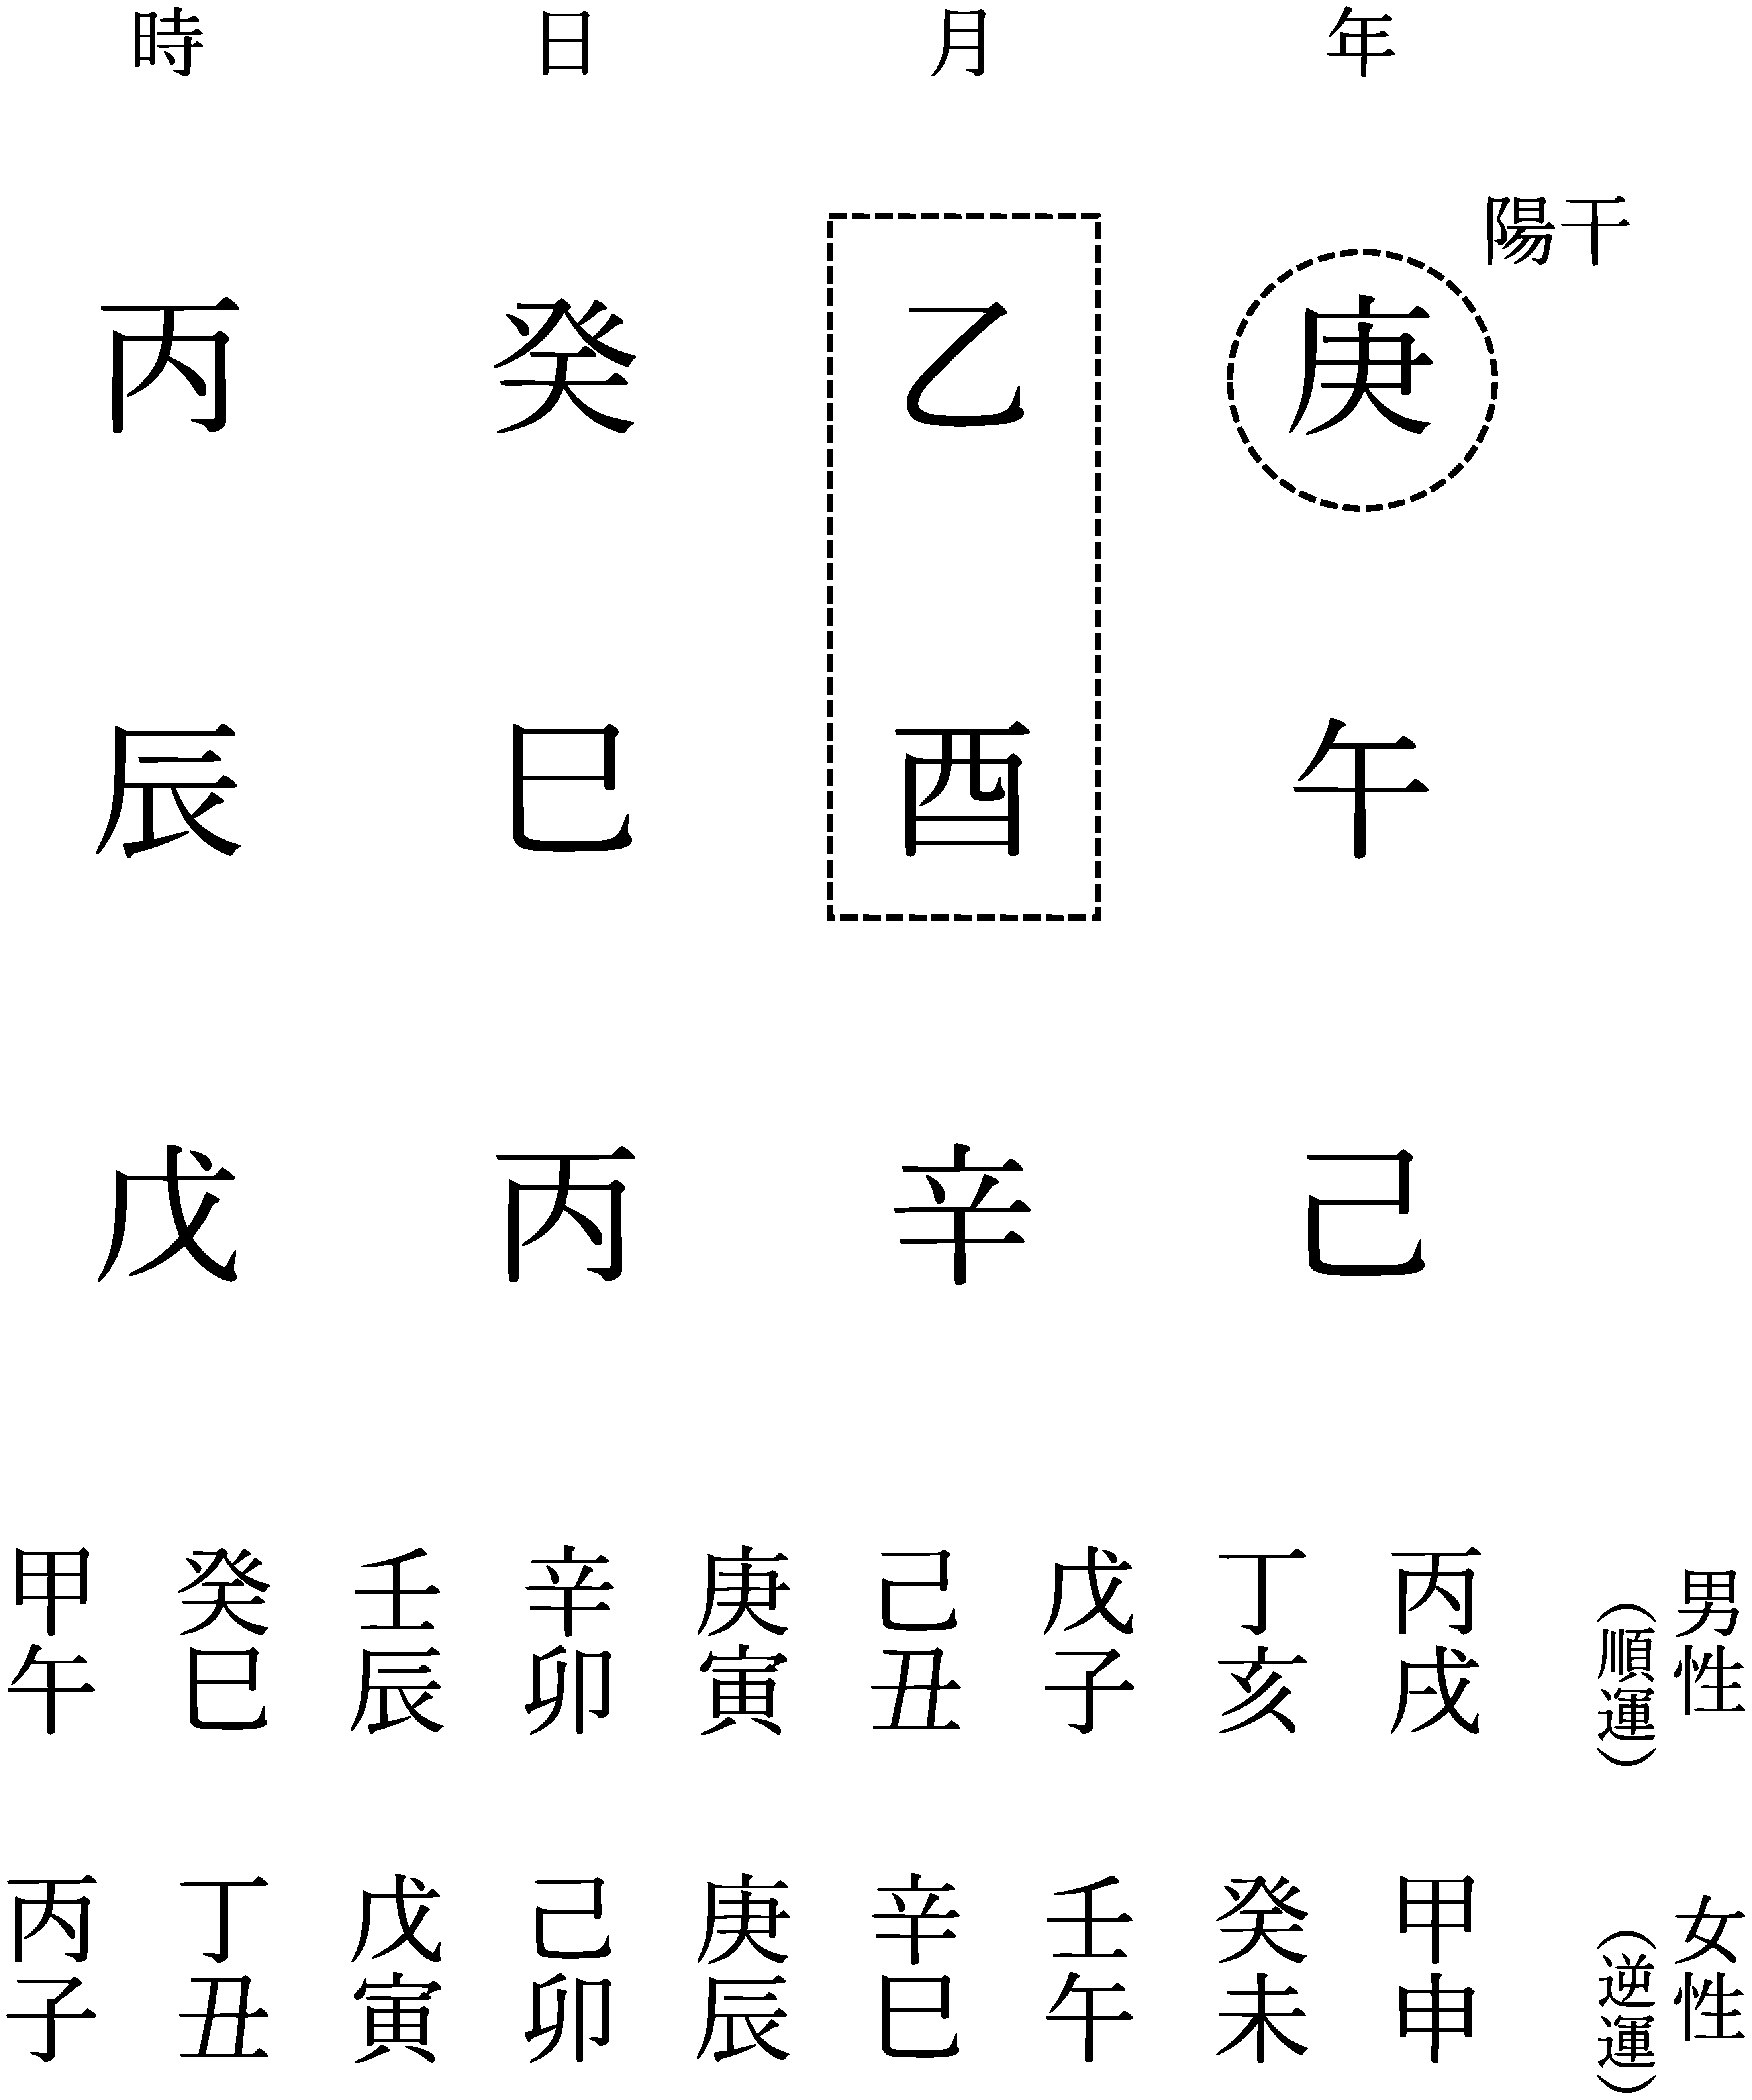
\includegraphics[width=60mm,angle=90]{figs/figure4-2.eps}
\end{figure}

まず、年柱天干「庚」は陽干のため、この命式の持ち主が男性であれば順運、女性であれば逆運です。

次に、干支を配置します。月柱の干支が大運の出発点となりますので、この場合は「乙酉」から出発します。六十干支表の「乙酉」を参照すると、男性(順運)であれば、大運は「丙戌」「丁亥」「戊子」「己丑」「庚寅」…と進んでいくことが分かります。逆に、女性(逆運)であれば、大運は「甲申」「癸未」「壬午」「辛巳」「庚辰」…と遡っていくことが分かります。\\

次の命式を用いてさらに説明します。

\begin{figure}[h]
  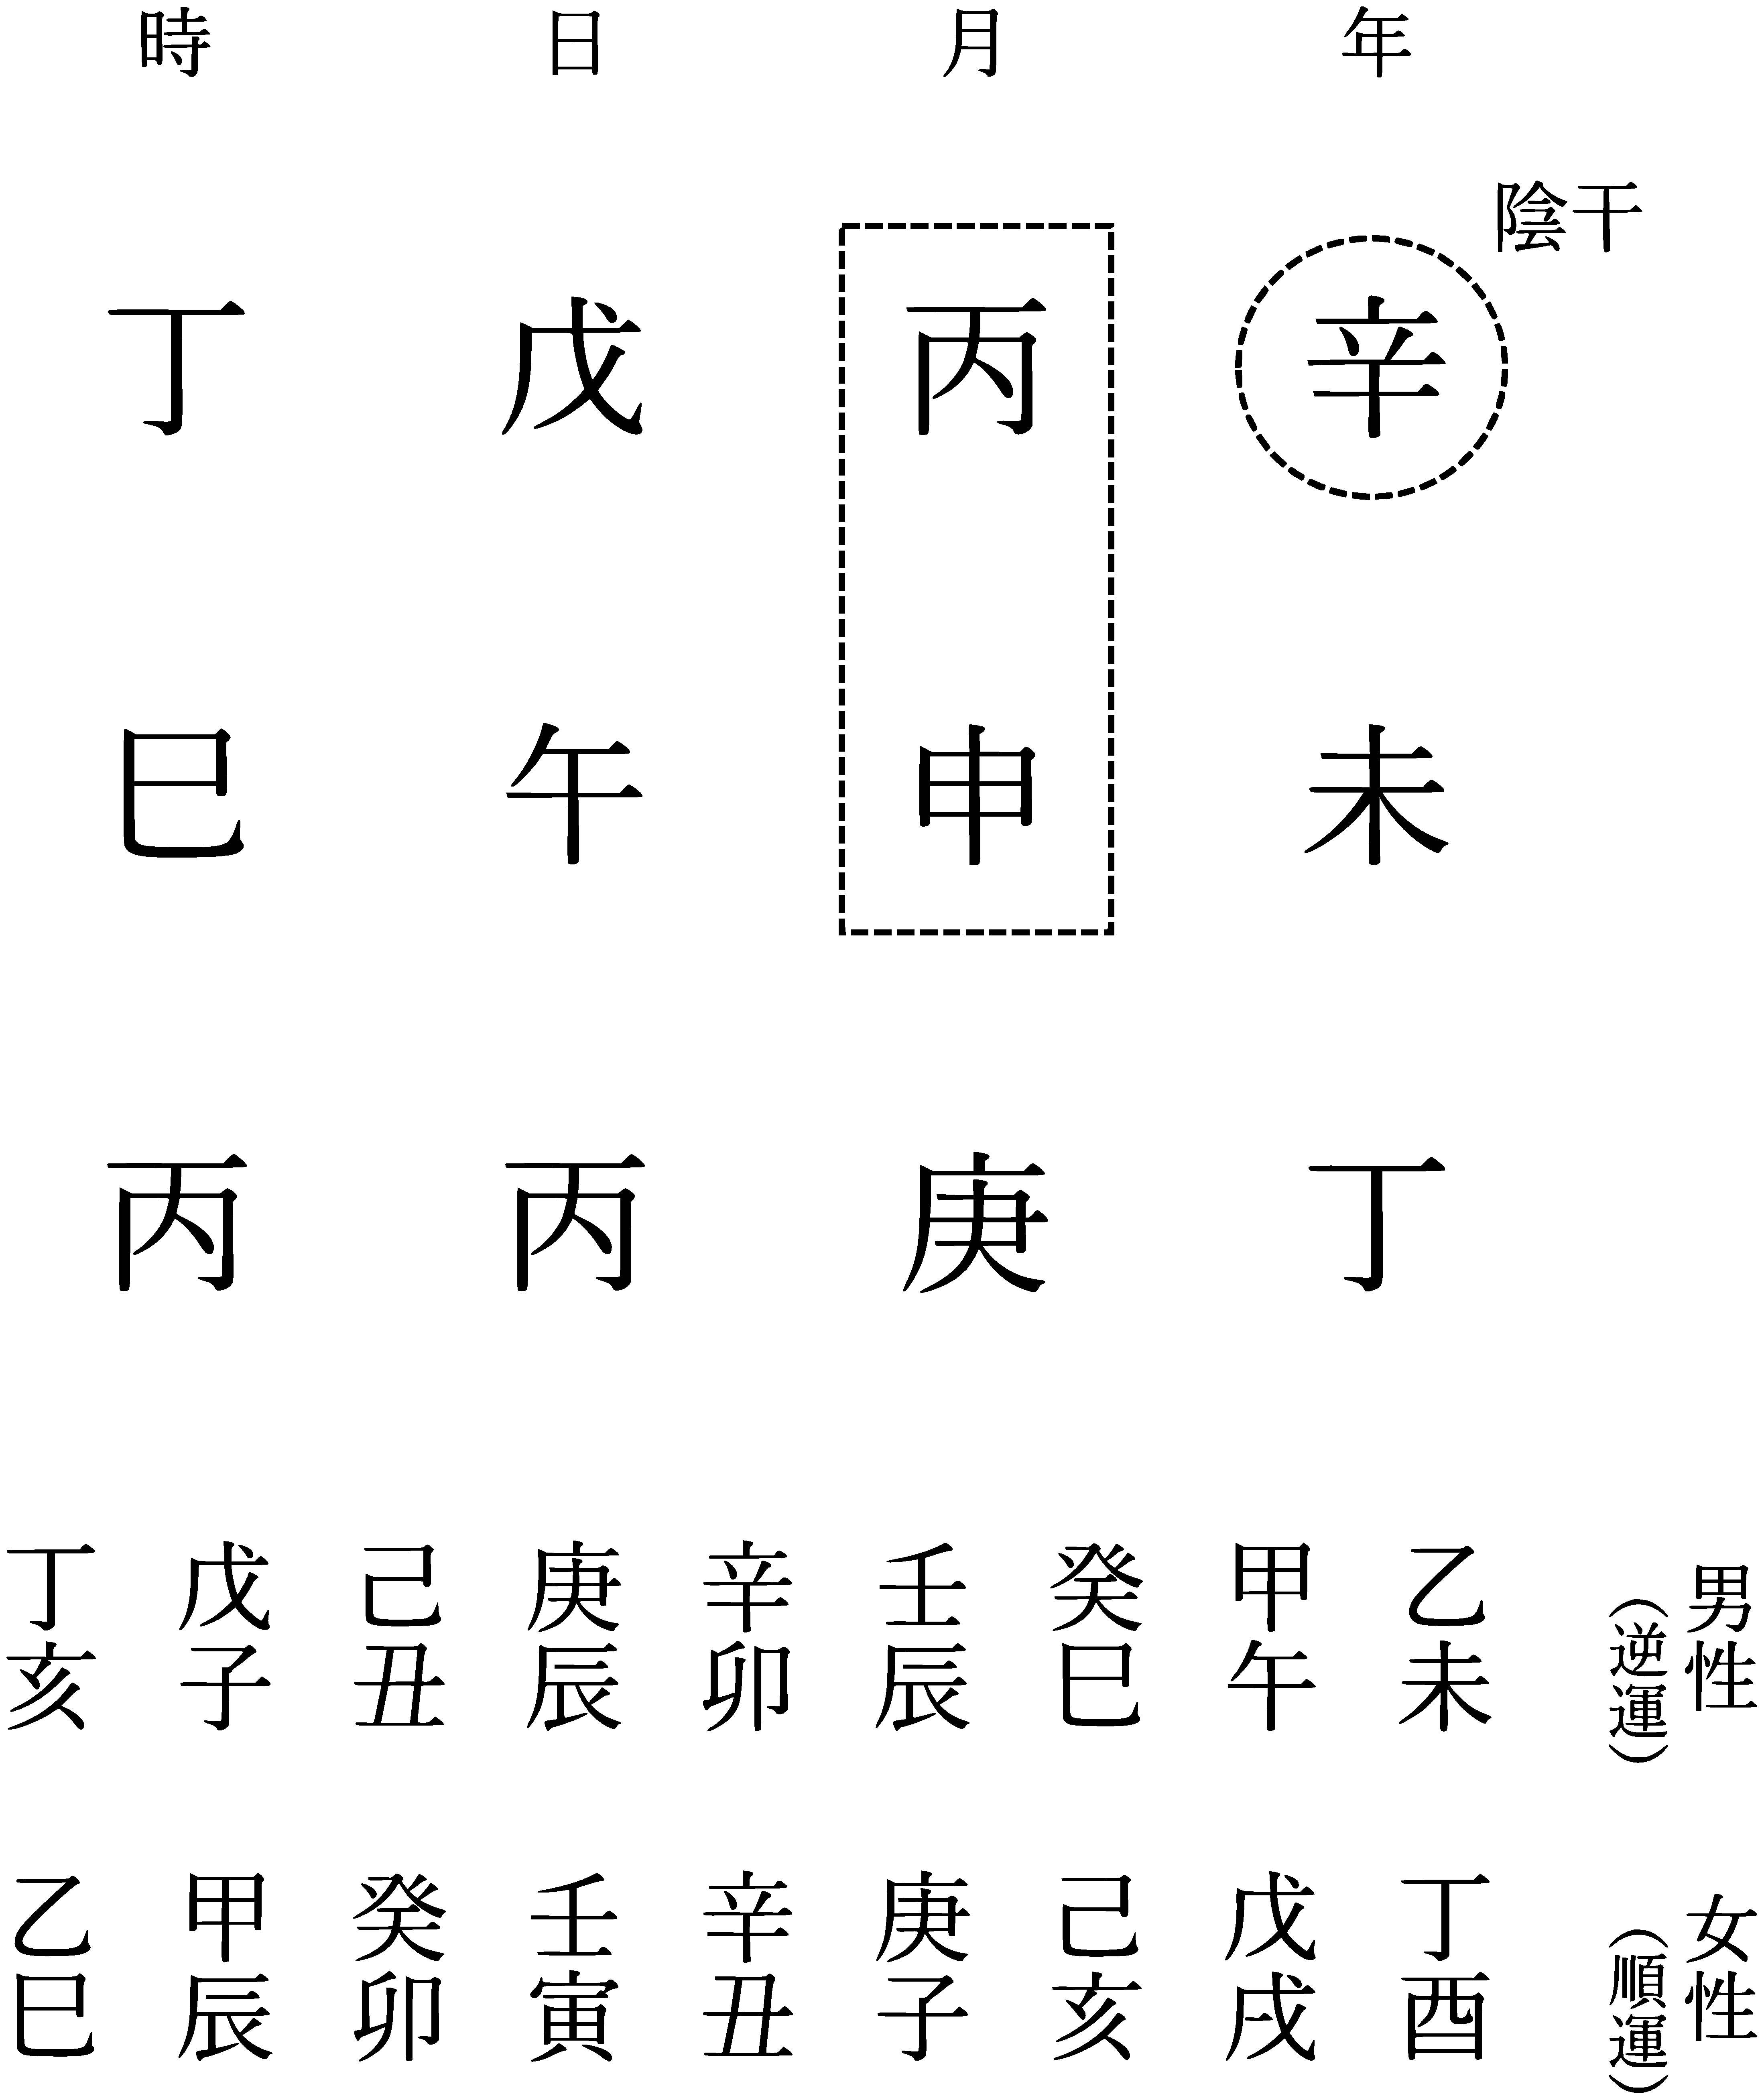
\includegraphics[width=60mm,angle=90]{figs/figure4-3.eps}
\end{figure}

まず、年柱天干「辛」は陰干のため、この命式の持ち主が男性であれば逆運、女性であれば順運です。

次に、干支を配置します。月柱の干支が大運の出発点となりますので、この場合は「丙申」から出発します。六十干支表の「丙申」を参照すると、男性(逆運)であれば、大運は「乙未」「甲午」「癸巳」「壬辰」「辛卯」…と遡っていくことが分かります。逆に、女性(順運)であれば、大運は「丁酉」「戊戌」「己亥」「庚子」「辛丑」…と進んでいくことが分かります。

\subsubsection*{立運計算}
次に、その人の大運が何歳から起算されるか(立運年数)を計算します。順運と逆運とで計算方法が異なるので、分けて説明します。\\

\noindent
(1)	順運の場合

生日より次の節入日までの日数を3で割り、1捨2入した数が立運年数となります。\footnote{3で割って1捨2入する詳しい理屈は、ここでは割愛します。}

平成\rensuji{13}年(2001年)\rensuji{10}月\rensuji{18}日\rensuji{17}時\rensuji{30}分生まれの女性を例にして、説明しましょう。

\begin{figure}[h]
  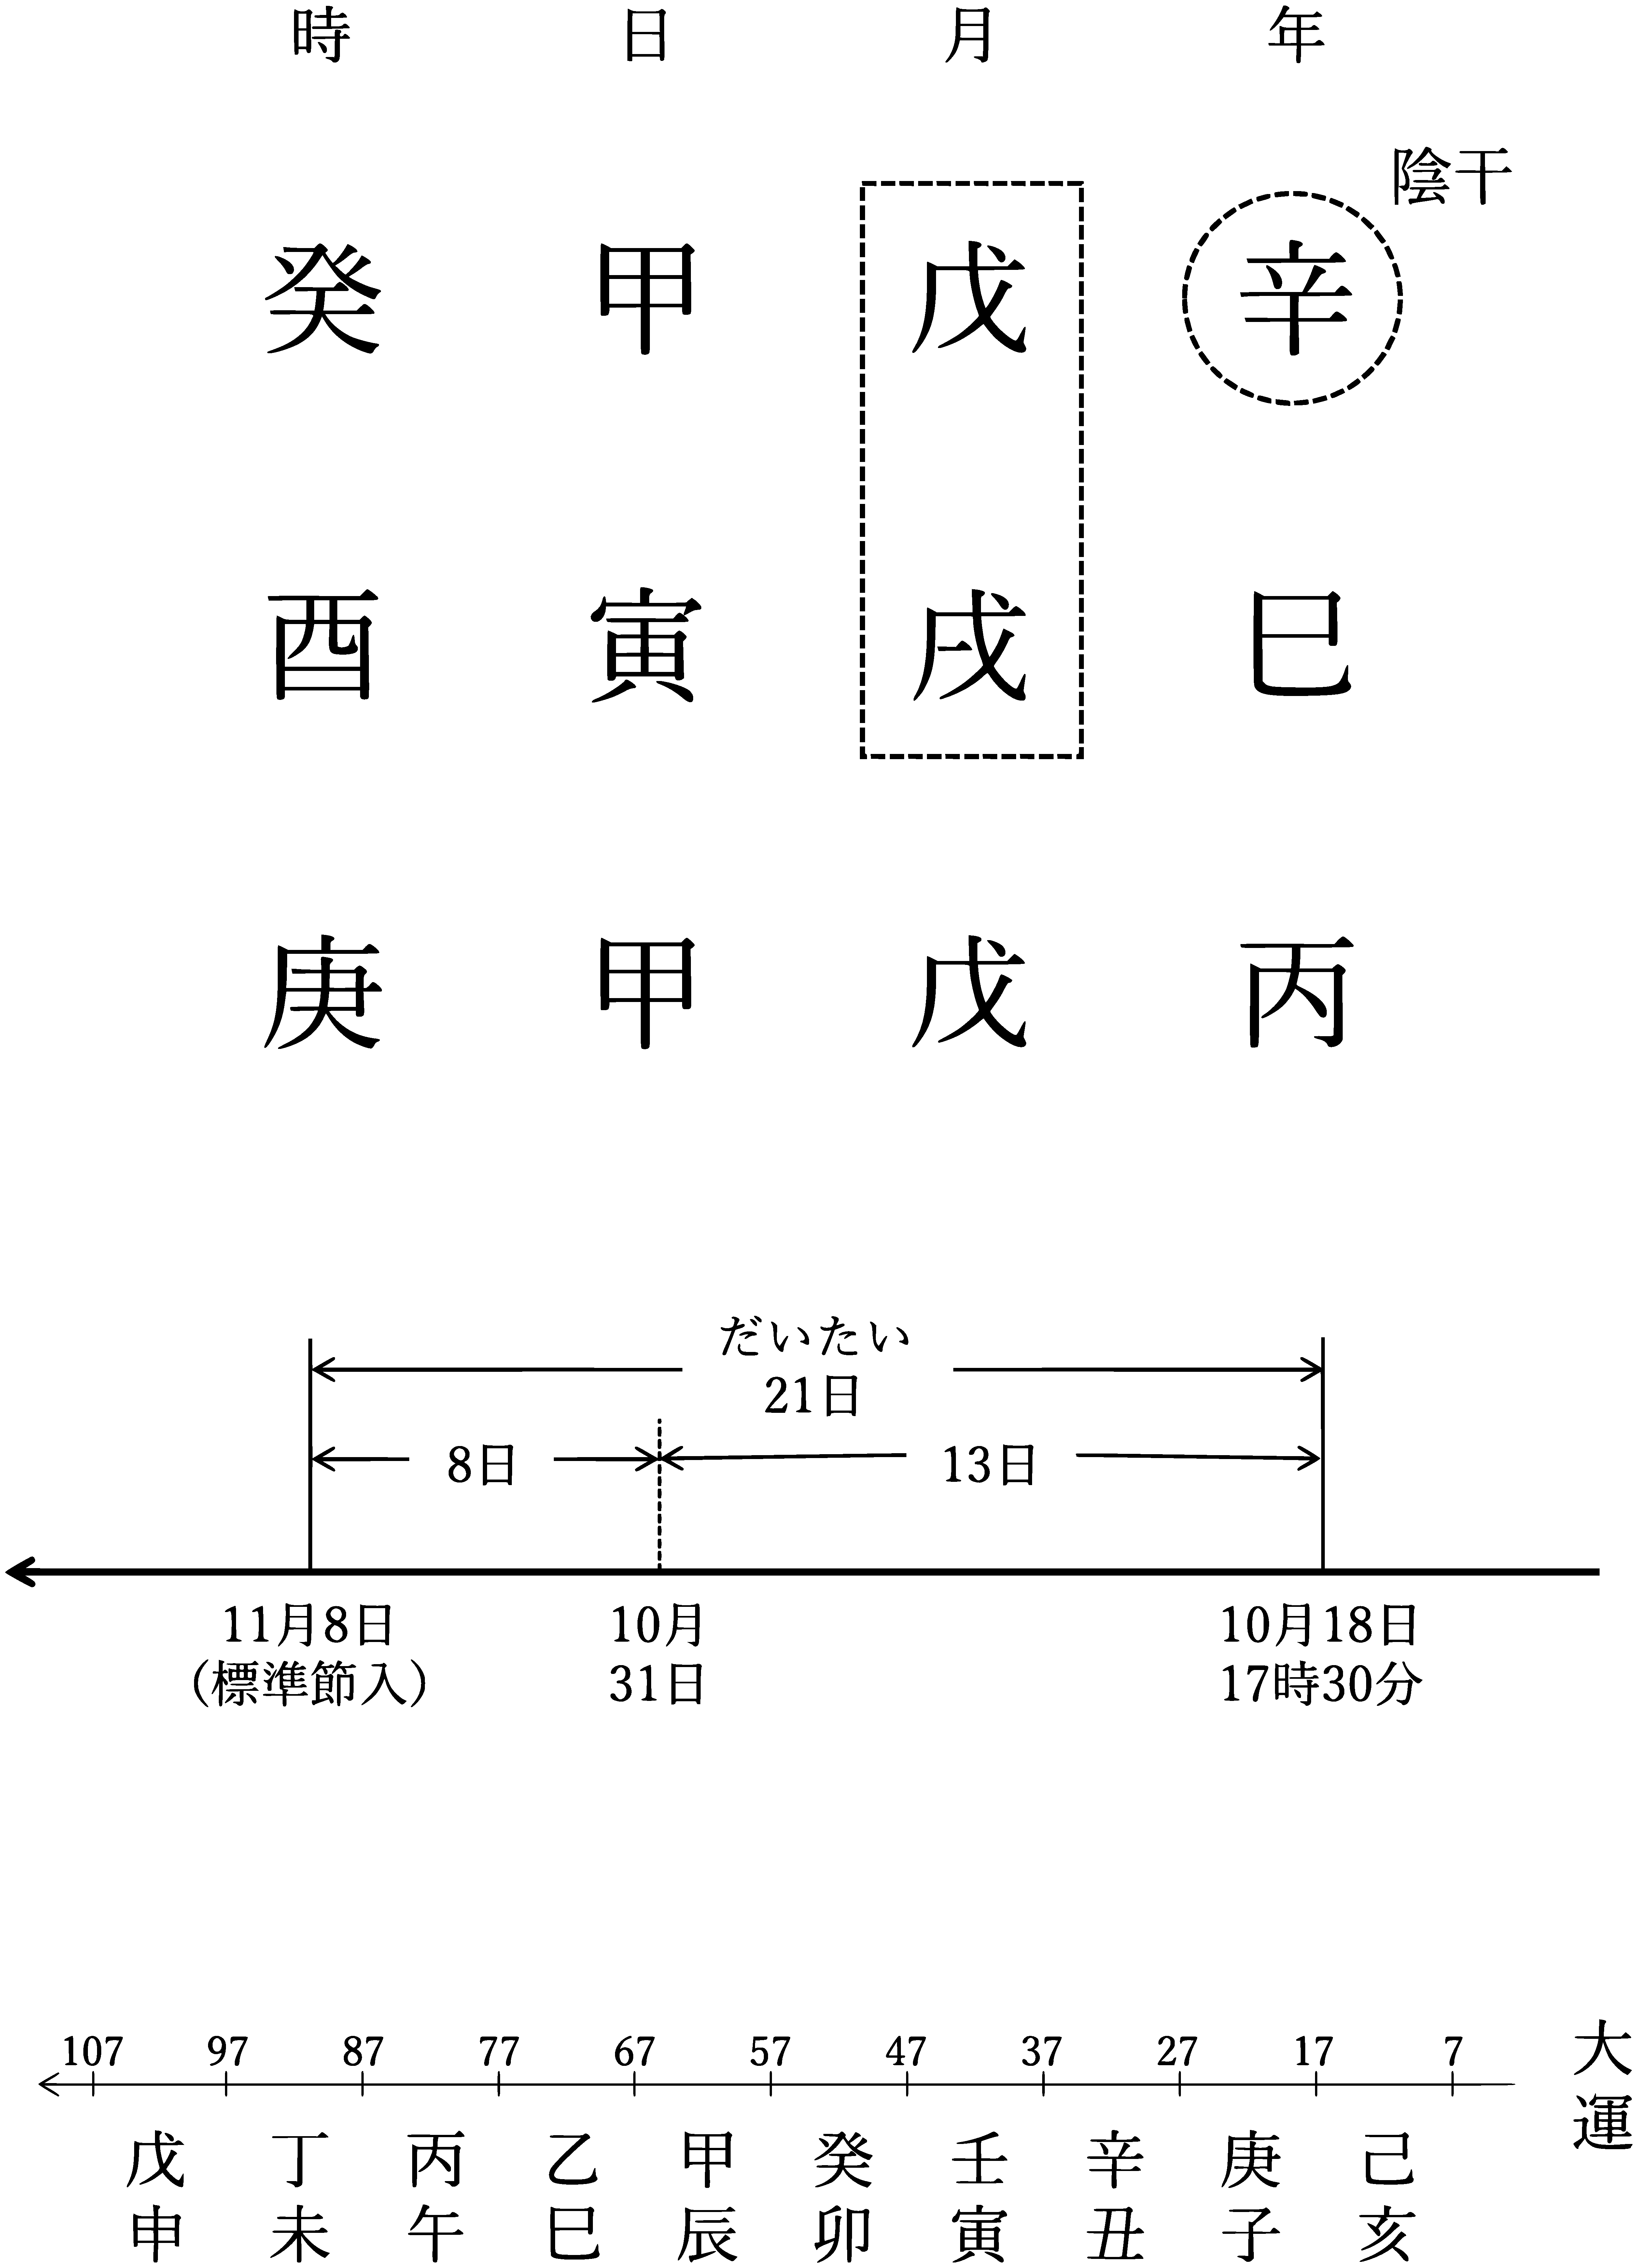
\includegraphics[width=60mm,angle=90]{figs/figure4-4.eps}
\end{figure}

まず、年柱天干に陰干「辛」を持つ女性のため、順運であることを確認します。次に、生日より次の節入日までの日数は、\rensuji{11}月の標準節入日(月干支表の○内数字を参照)を考慮すると「だいたい\rensuji{21}日」であることが分かります。そして、これを3で割ると「7余り0」となるため、立運年数は「7年」と計算できます。

月柱干支は「戊戌」ですから、六十干支表の「戊戌」を参照します。順運ですから、大運は「戊戌」の次の干支「己亥」から順番に進んでいきます。結果、この女性の大運は、右図下のとおりとなります。

\noindent
\\(2) 逆運の場合

生日より前の節入日までの日数を3で割り、1捨2入した数が立運年数となります。

平成4年(1992年)7月4日7時\rensuji{20}分生まれの女性を例にして説明しましょう。

\begin{figure}[h]
  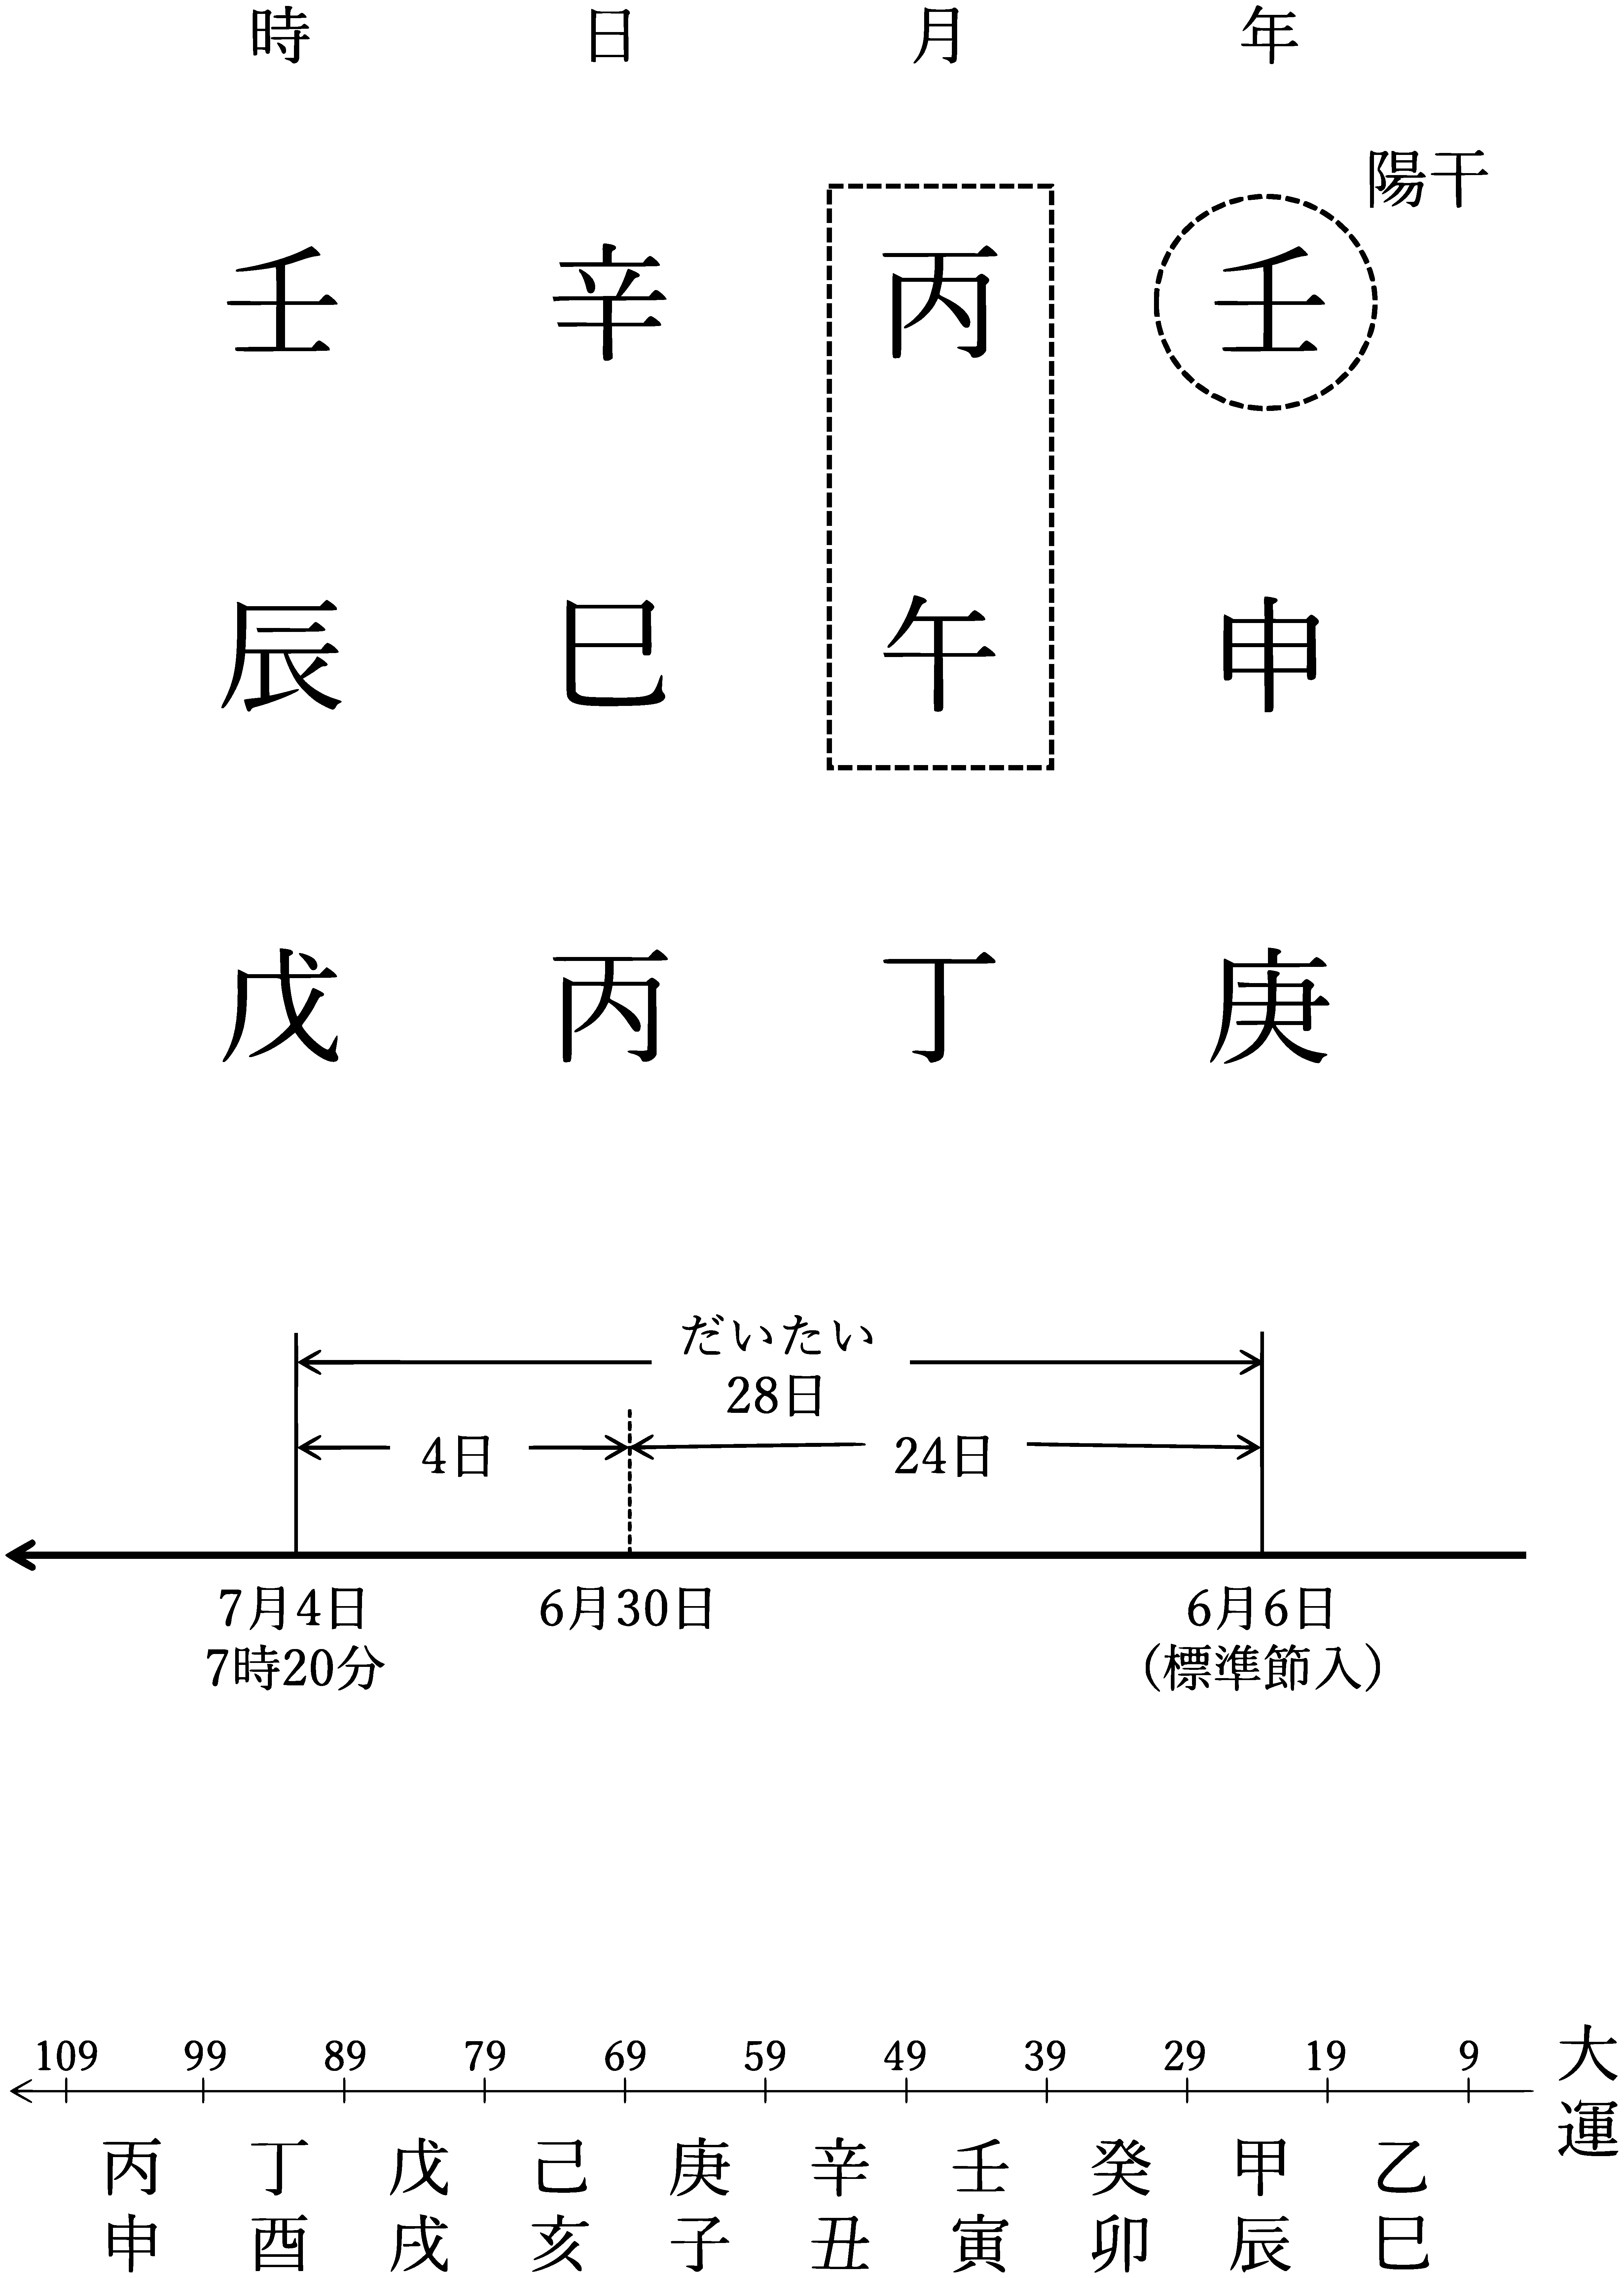
\includegraphics[width=60mm,angle=90]{figs/figure4-6.eps}
\end{figure}

まず、年柱天干に陽干「壬」を持つ女性のため、逆運であることを確認します。次に、生日より前の節入日までの日数は、6月の標準節入日を考慮すると「だいたい\rensuji{28}日」であることが分かります。そして、これを3で割ると「9余り1」となるため、立運年数は「9年」と計算できます(余りの1は切り捨てます)。

月柱干支は「丙午」ですから、六十干支表の「丙午」を参照します。逆運ですから、大運は「丙午」の前の干支「乙巳」から順番に遡っていきます。結果、この女性の大運は、右図下のとおりとなります。\\

大運は、その人が生涯歩いていかなければならない人生の道であり、運勢の起伏になります。
一〇年ごとの運勢は、四柱命式と大運との組み合わせによって推測します。

\subsection{年運}
干支暦では、六十干支表にしたがって暦(干支)が巡ることを第二章で説明しました。四柱推命学においては、運勢を読むためにこの年の干支も重要で、これを\ruby{年運}{ねんうん}と呼びます。

大運は人それぞれ異なりますが、年運はすべての人に共通です。例えば、令和5年は「癸卯」の年であり、令和6年は「甲辰」の年でした。各年の運勢は、四柱命式と大運・年運との組み合わせによって推測します。

つまり、先天運命(性格や人事・事相など)は四柱(生年・月・日・時)で推命するのに対し、後天運勢は六柱(生年・月・日・時・大運・年運)で推測することになります。

生年・月・日・時から構成された四柱命式は、持って生まれた宿命的なものです。
その宿命的運命が生涯にわたって変化する過程をみるのが大運・年運で、その動きをよく把握しながら、
個人の努力によって「禍転じて福にする」ことも不可能ではありません。
先天的宿命は如何ともし難いのですが、これを知って努力するのは後天的人力によるものです。

\subsection{接木運}

\begin{wrapfigure}{l}[0pt]{0.3\textwidth}
  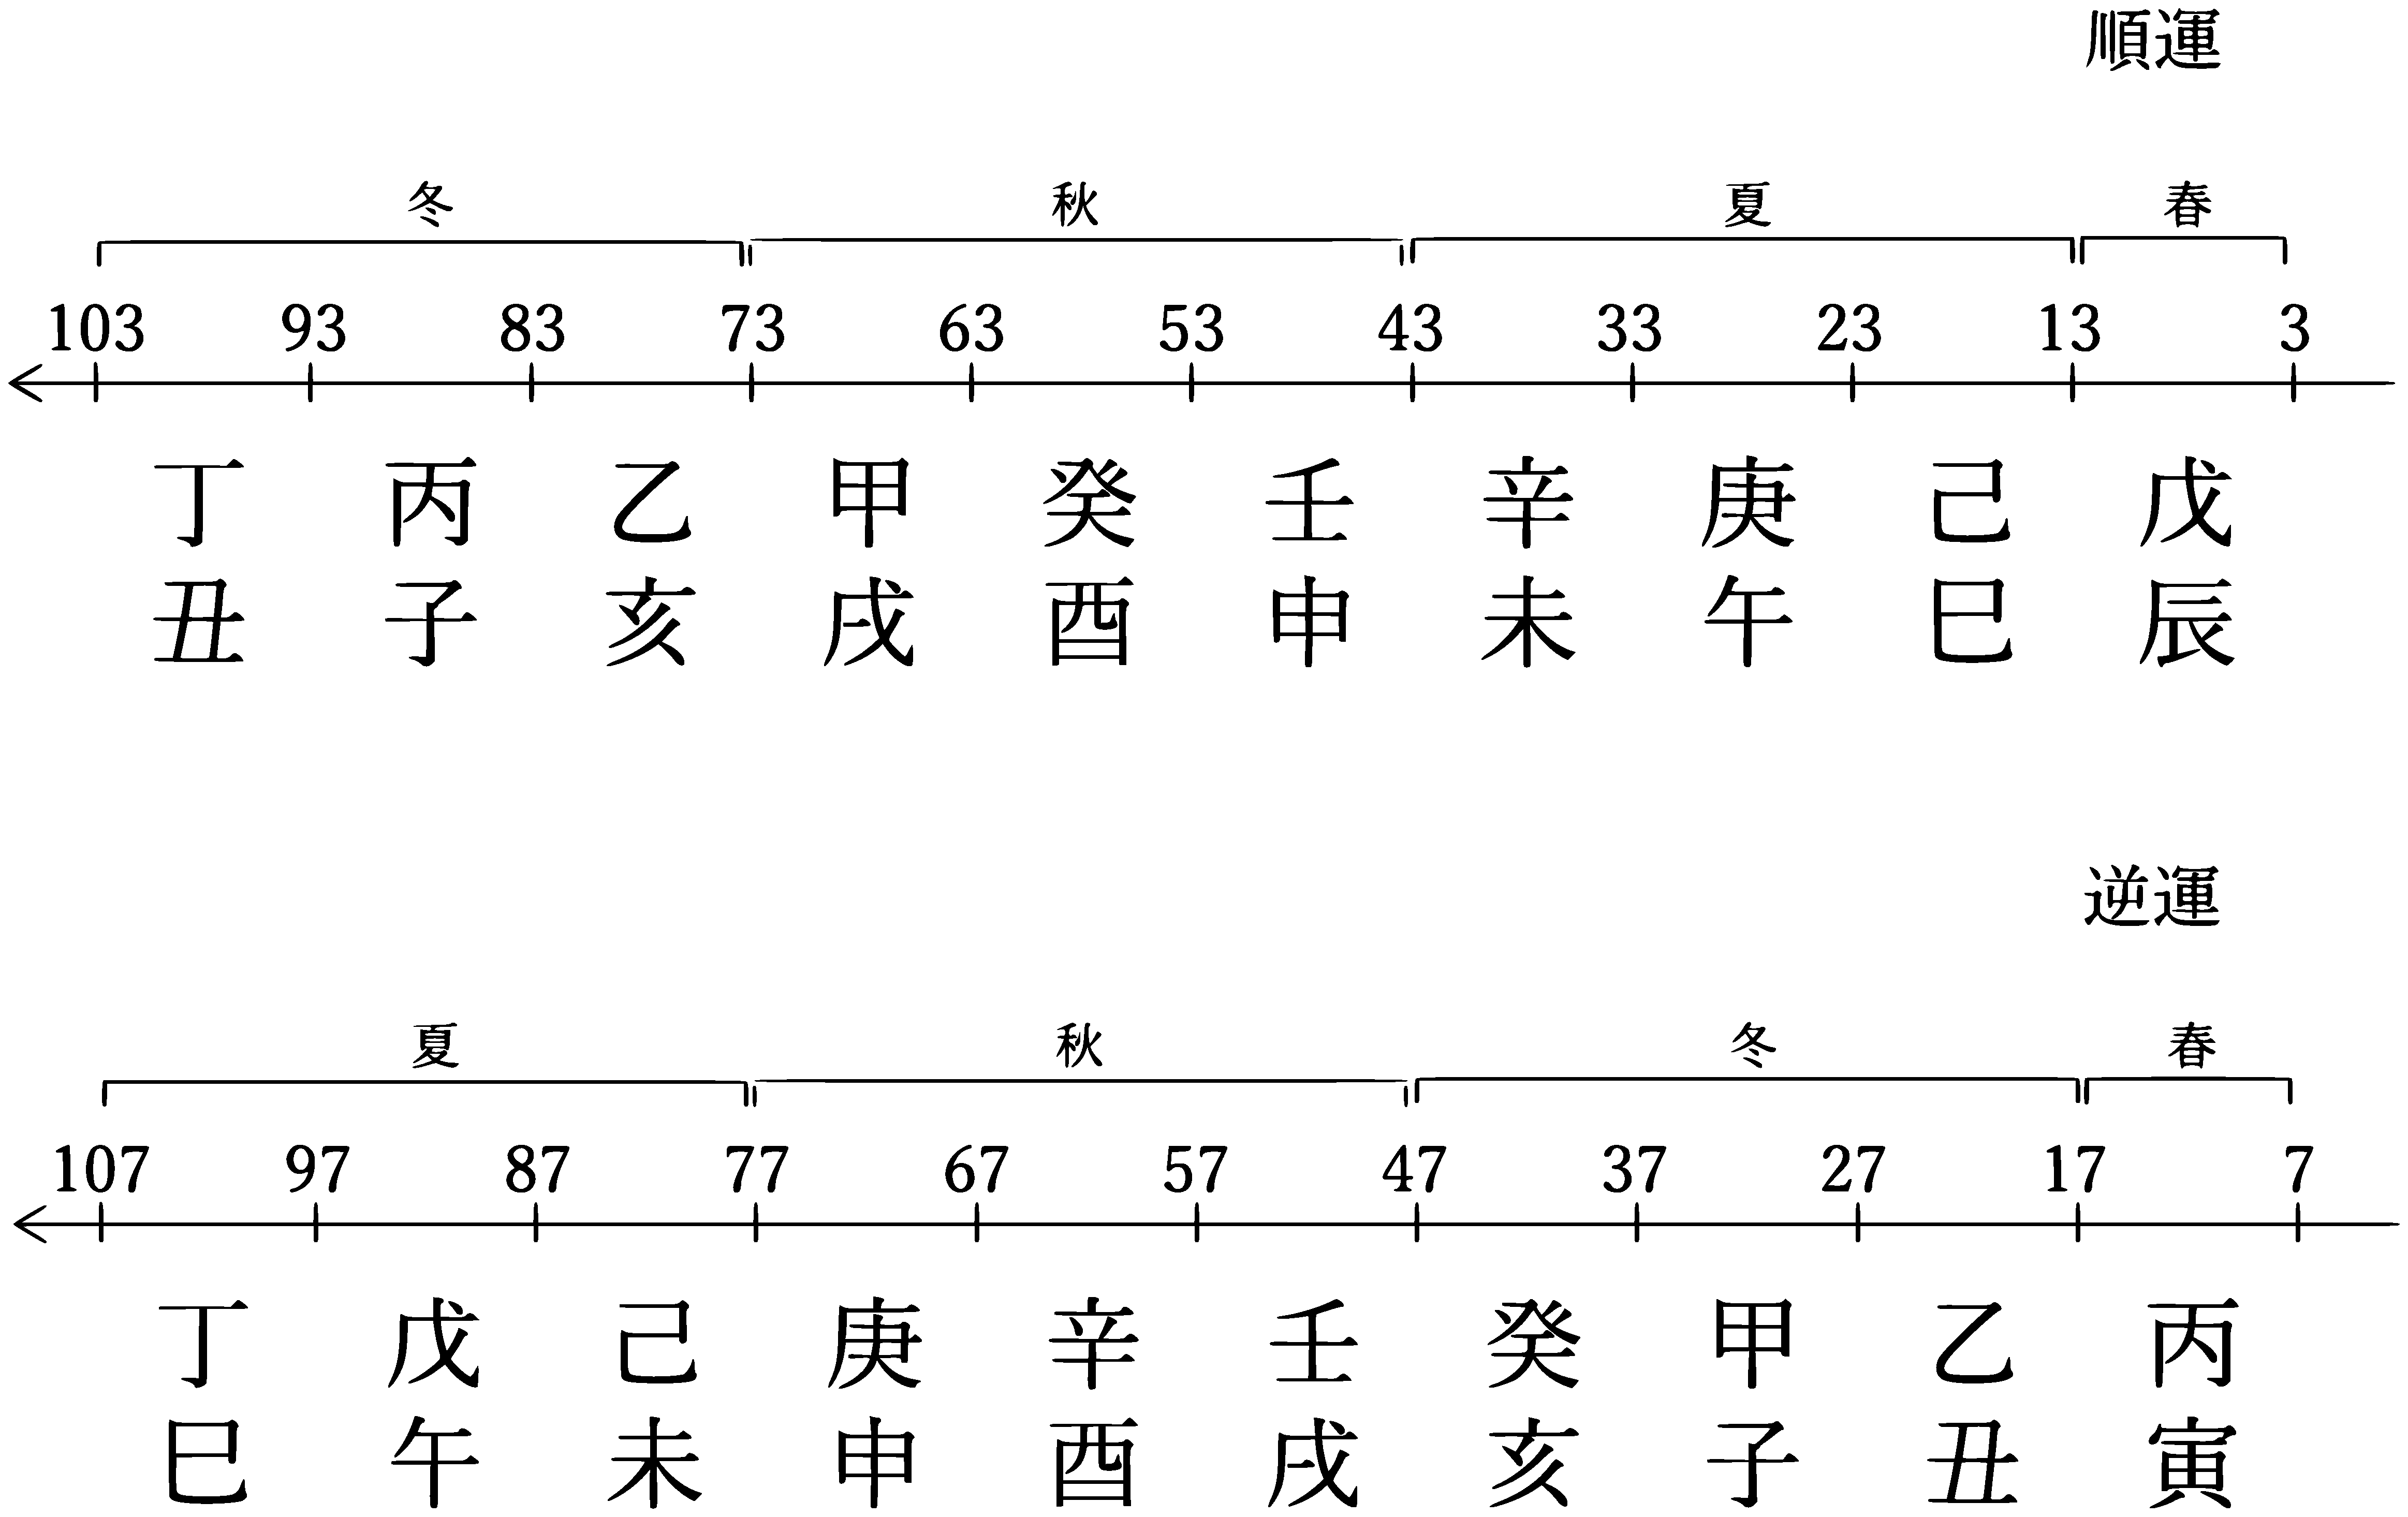
\includegraphics[width=75mm,angle=90]{figs/figure4-8.eps}
\end{wrapfigure}

大運の支を四季に分けて区切りをつけると、三〇年ごとに季節が変わっていくことになります。つまり、寅\rensuji{10}年・卯\rensuji{10}年・辰\rensuji{10}年の\rensuji{30}年が春、巳・午・未が夏、申・酉・戌が秋、亥・子・丑が冬です。そして、大運における季節の変わり目を「\ruby{接木運}{せつぼくうん}」といいます。\footnote{辰・未・戌・丑が、それぞれ春・夏・秋・冬を兼ねることに注意が必要です。つまり、辰は「春・土用」(木の土)、未は「夏・土用」(火の土)、戌は「秋・土用」(金の土)、丑は「冬・土用」(水の土)であり、例えば、辰は「土用」であると同時に「春」になります。}

上の図で説明します。

図の上の大運(順運)の場合、3歳から\rensuji{12}歳までが春(辰)、\rensuji{13}歳から\rensuji{42}歳までが夏(巳・午・未)、\rensuji{43}歳から\rensuji{72}歳までが秋(申・酉・戌)、\rensuji{73}歳以降が冬(亥・子・丑)です。そして、\rensuji{13}歳前後・\rensuji{43}歳前後・\rensuji{73}歳前後が接木運になります。

図の下の大運(逆運)の場合、7歳から\rensuji{16}歳までが春(辰)、\rensuji{17}歳から\rensuji{46}歳までが冬(丑・子・亥)、\rensuji{47}歳から\rensuji{76}歳までが秋(戌・酉・申)、\rensuji{77}歳以降が夏(未・午・巳)です。そして、\rensuji{17}歳前後・\rensuji{47}歳前後・\rensuji{77}歳前後が接木運になります。

私たちの身体でも、気候の変わり目は調子が悪くなることがあるように、この接木運にあたる年の前後は、あらゆることに注意を必要とします。
人によっては、運勢上に大きな変化をもたらす年まわりになることが多いと考えられています。



\clearpage

\section{通変}

\ruby{通変}{つうへん}は、二つの干の陰陽五行の関係を二字熟語で表現したものです。通変には、\ruby{比肩}{ひけん}、\ruby{劫財}{ごうざい}、\ruby{食神}{しょくじん}、\ruby{傷官}{しょうかん}、\ruby{偏財}{へんざい}、\ruby{正財}{せいざい}、\ruby{偏官}{へんかん}、\ruby{正官}{せいかん}、\ruby{偏印}{へんいん}、\ruby{印綬}{いんじゅ}の十種類があります。それぞれの意味を説明する前に、まずは「五行の\ruby{生剋}{しょうこく}関係」について解説します。

\subsection{五行の生剋}
五行の各要素の間には相対的な関係があります。\ruby{木}{もく}\ruby{火}{か}\ruby{土}{ど}\ruby{金}{ごん}\ruby{水}{すい}の並びにおいて、互いに隣り合う五行の間には、「\ruby{生}{しょう}」の関係があります。具体的には、

\begin{wrapfigure}{l}[0pt]{0.25\textwidth}
  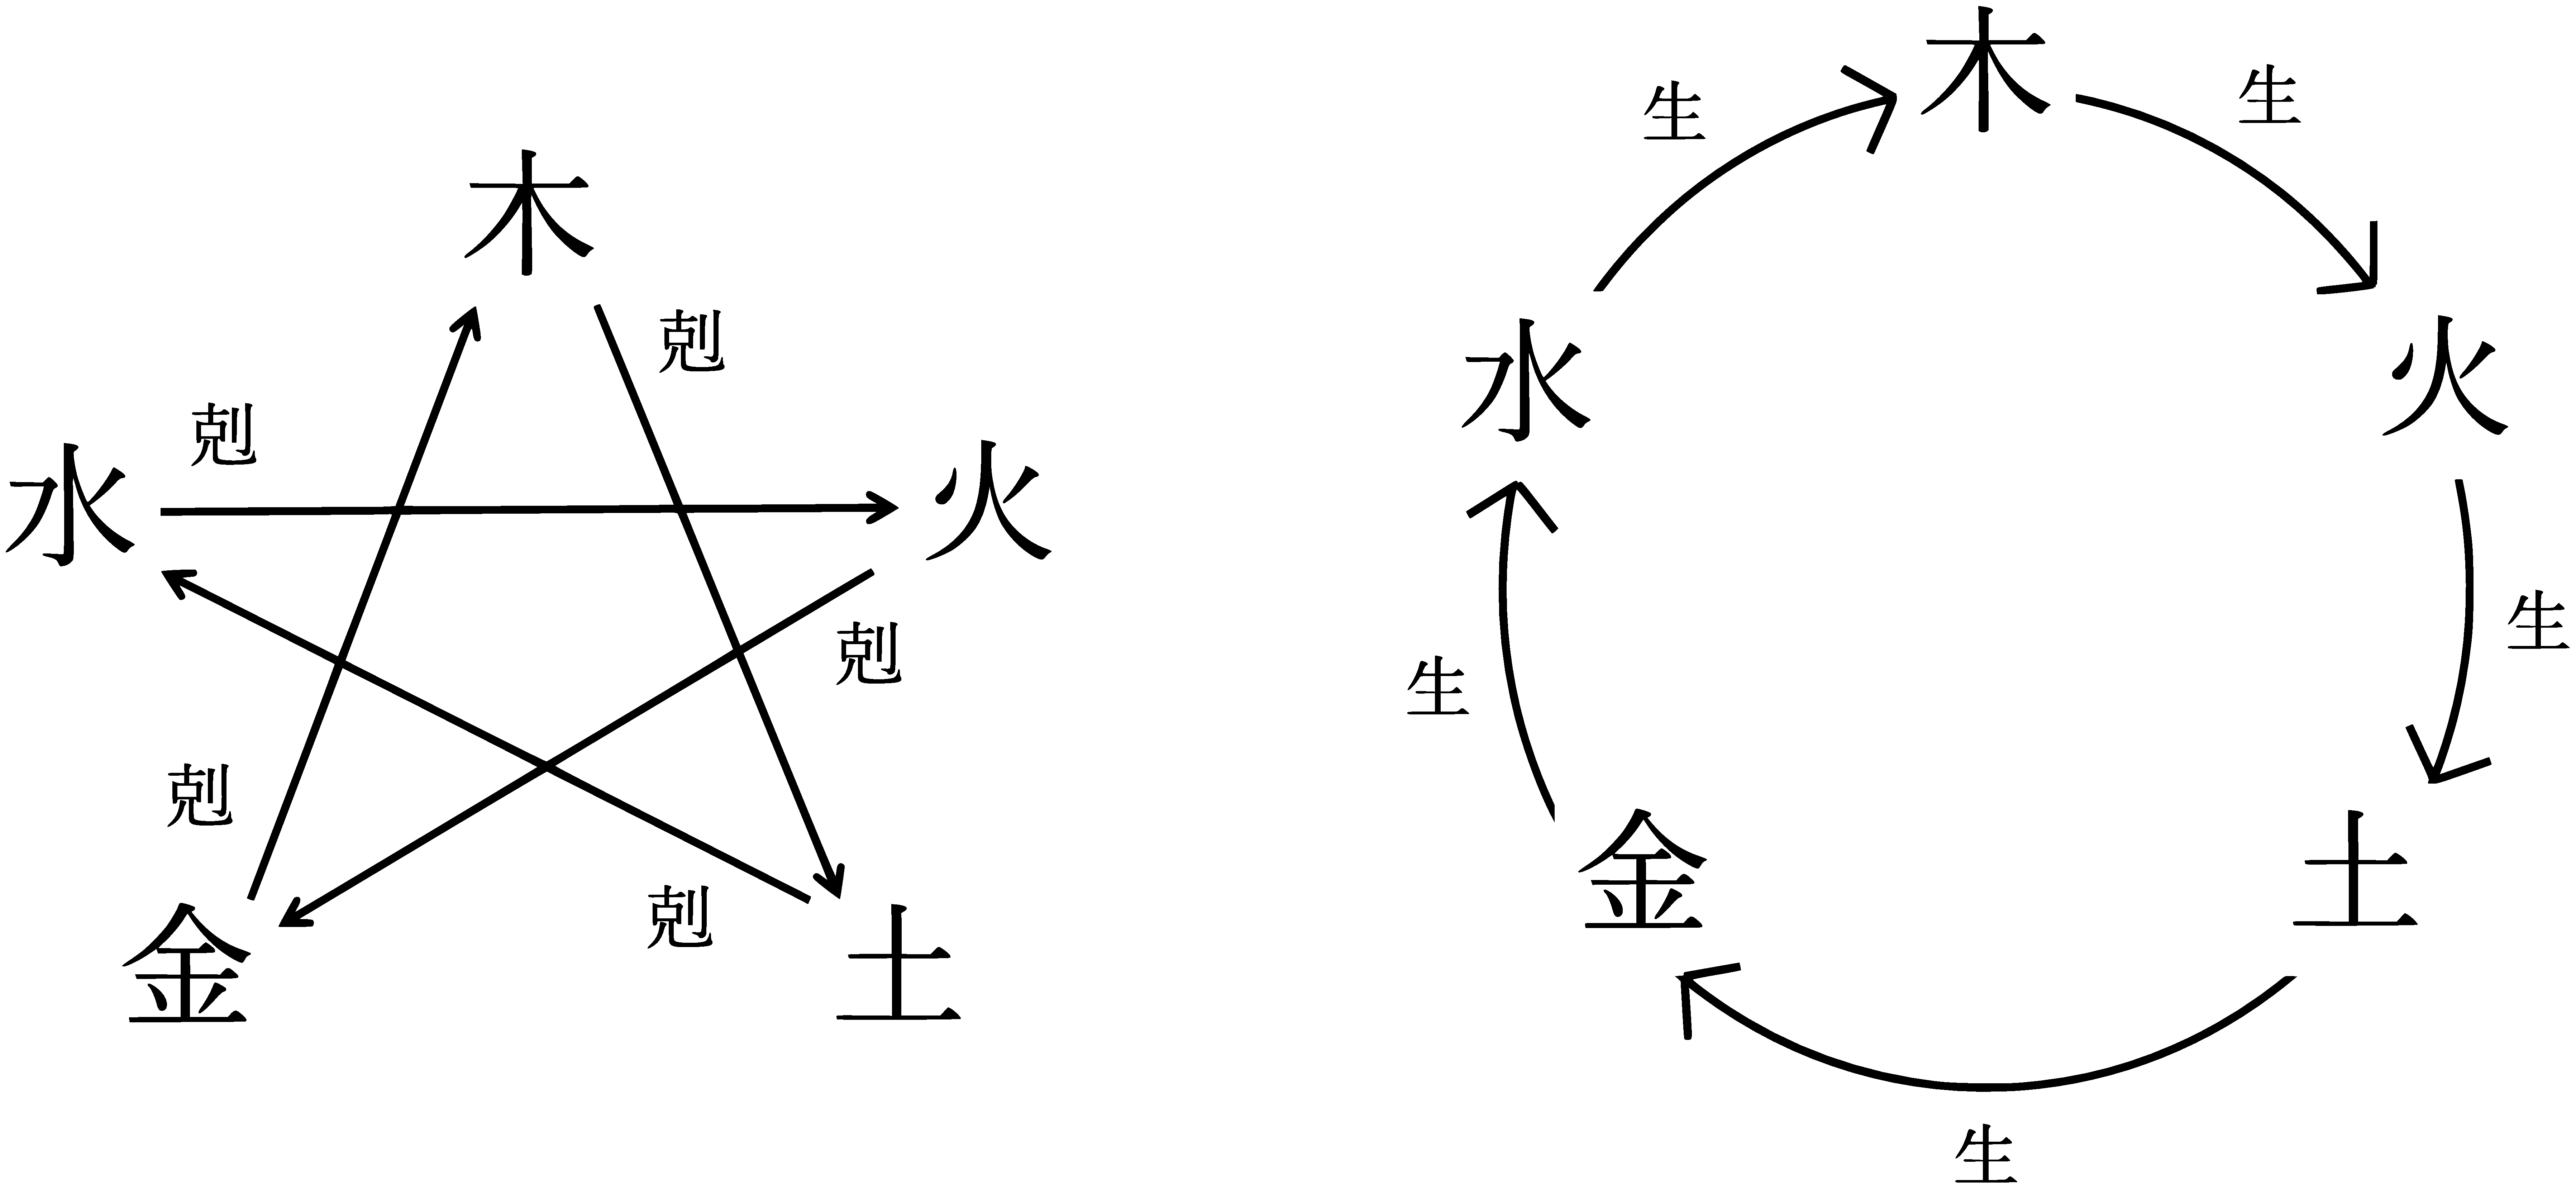
\includegraphics[width=90mm,angle=90]{figs/figure5-1.eps}
\end{wrapfigure}

\begin{itemize}
\item 木は燃えて火を生じ(\ruby{木生火}{もくしょうか})
\item 火は灰となって土を生じ(\ruby{火生土}{かしょうど})
\item 土は固まって金を生じ(\ruby{土生金}{どしょうきん})
\item 金は冷えて水を生じ(\ruby{金生水}{きんしょうすい})
\item 水は木を育て生じる(\ruby{水生木}{すいしょうもく})
\end{itemize}
という関係があります。

一方、\ruby{木}{もく}\ruby{火}{か}\ruby{土}{ど}\ruby{金}{ごん}\ruby{水}{すい}の並びにおいて、一つ飛ばして二つ先の五行、および、二つ飛ばして三つ先の五行との間には、「\ruby{剋}{こく}」の関係があります。具体的には、
\begin{itemize}
\item 木は土から養分を吸い上げ(\ruby{木剋土}{もっこくど})
\item 火は金を溶解し(\ruby{火剋金}{かこくきん})
\item 土は水の流れをせき止め(\ruby{土剋水}{どこくすい})
\item 金は尖って木を切り倒し(\ruby{金剋木}{きんこくもく})
\item 水は火を消す(\ruby{水剋火}{すいこくか})
\end{itemize}  
という関係があります。\\

いま「木」を基準にして考えると、「火」は「生じる五行」であり(\ruby{木生火}{もくしょうか})、「土」は「剋す五行」であり(\ruby{木剋土}{もっこくど})、「金」は「剋される五行」であり(\ruby{金剋木}{きんこくもく})、「水」は「生じられる五行」です(\ruby{水生木}{すいしょうもく})。

\begin{figure}[h]
  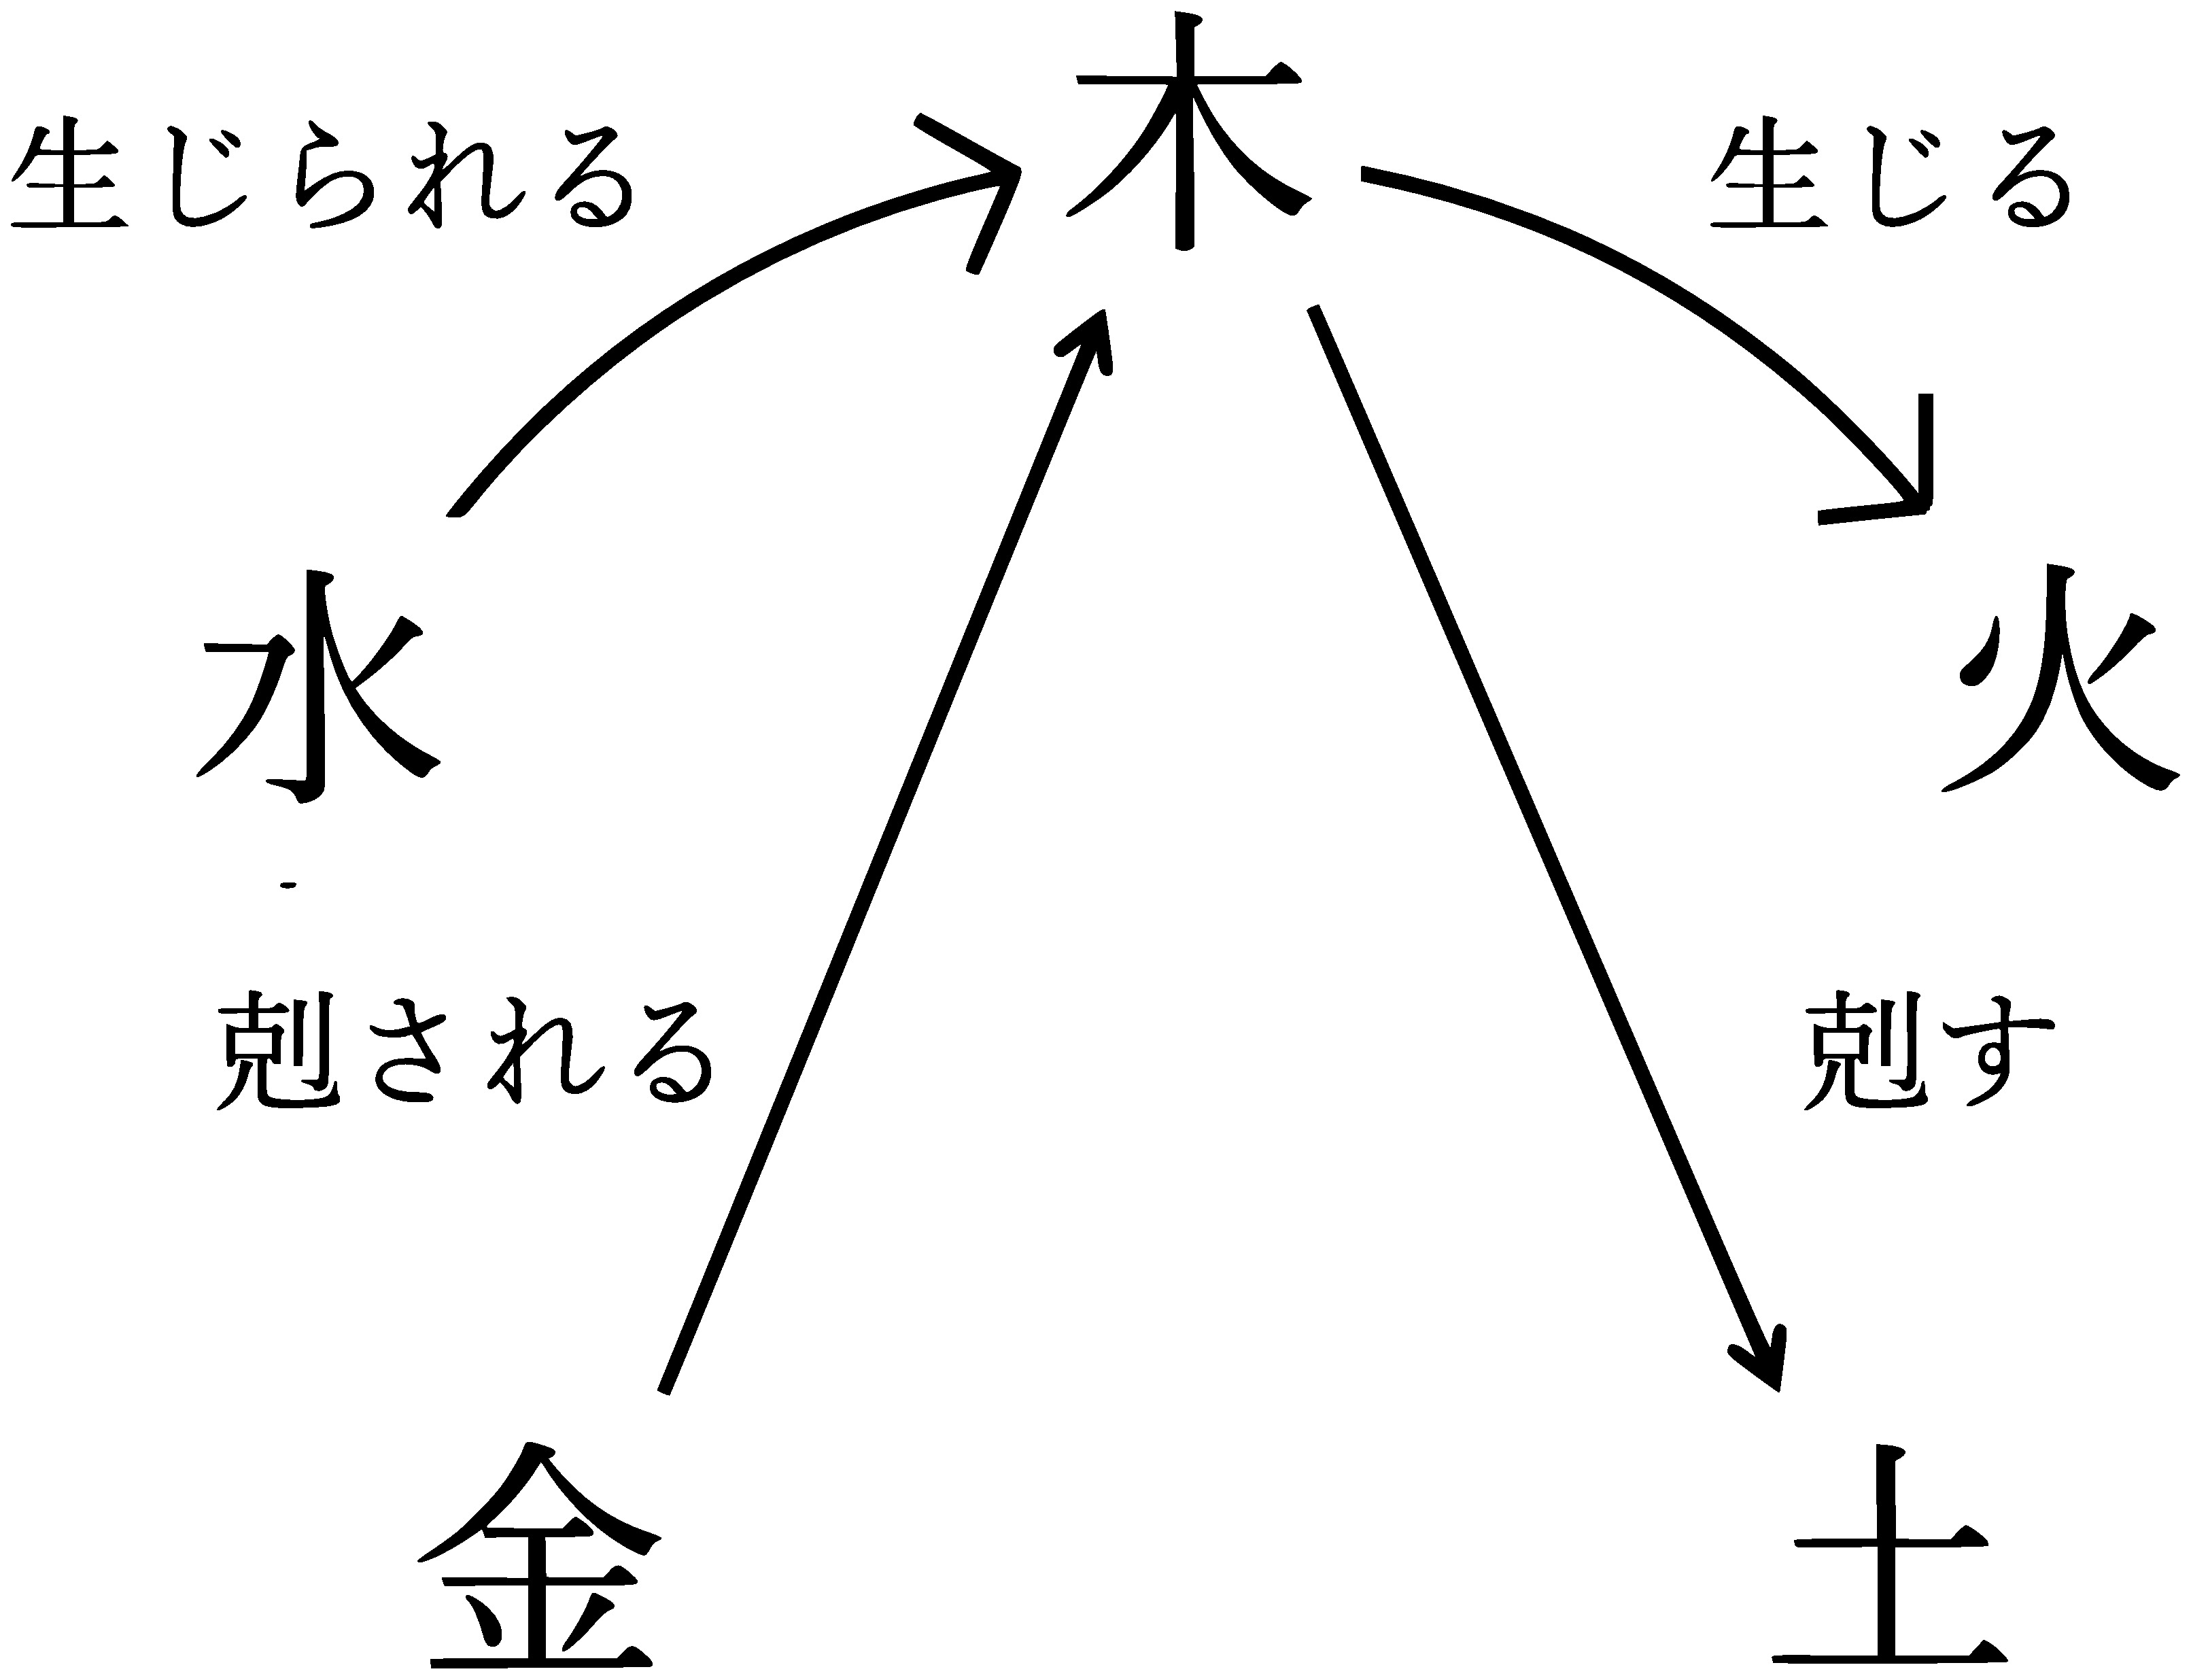
\includegraphics[width=45mm,angle=90]{figs/figure5-3.eps}
\end{figure}

なお、「木」を基準にした場合、「木」は「同一の五行」であり、これを「\ruby{比和}{ひわ}」の関係といいます。

\subsection{通変の成り立ち}

二つの干があったとき、一方の干から見て、他方の干の陰陽五行を二字熟語で整理したものが「通変」です。

例えば、「甲」を基準として「丙」の通変を考えると、甲(木)にとって丙(火)は「生じる五行」であり(\ruby{木生火}{もくしょうか})、陰陽は「陽」と「陽」で同じです。この場合、丙の通変は「\ruby{食神}{しょくじん}」になります。

同様に「辛」を考えると、甲(木)にとって辛(金)は「剋される五行」であり(\ruby{金剋木}{きんこくもく})、陰陽は「陽」と「陰」で異なります。この場合、辛の通変は「\ruby{正官}{せいかん}」になります。

さらに「乙」を考えると、甲(木)にとって乙(木)は「同一の五行」であり、陰陽は「陽」と「陰」で異なります。この場合、乙の通変は「\ruby{劫財}{ごうざい}」になります。

\begin{wrapfigure}{l}[0pt]{0.25\textwidth}
  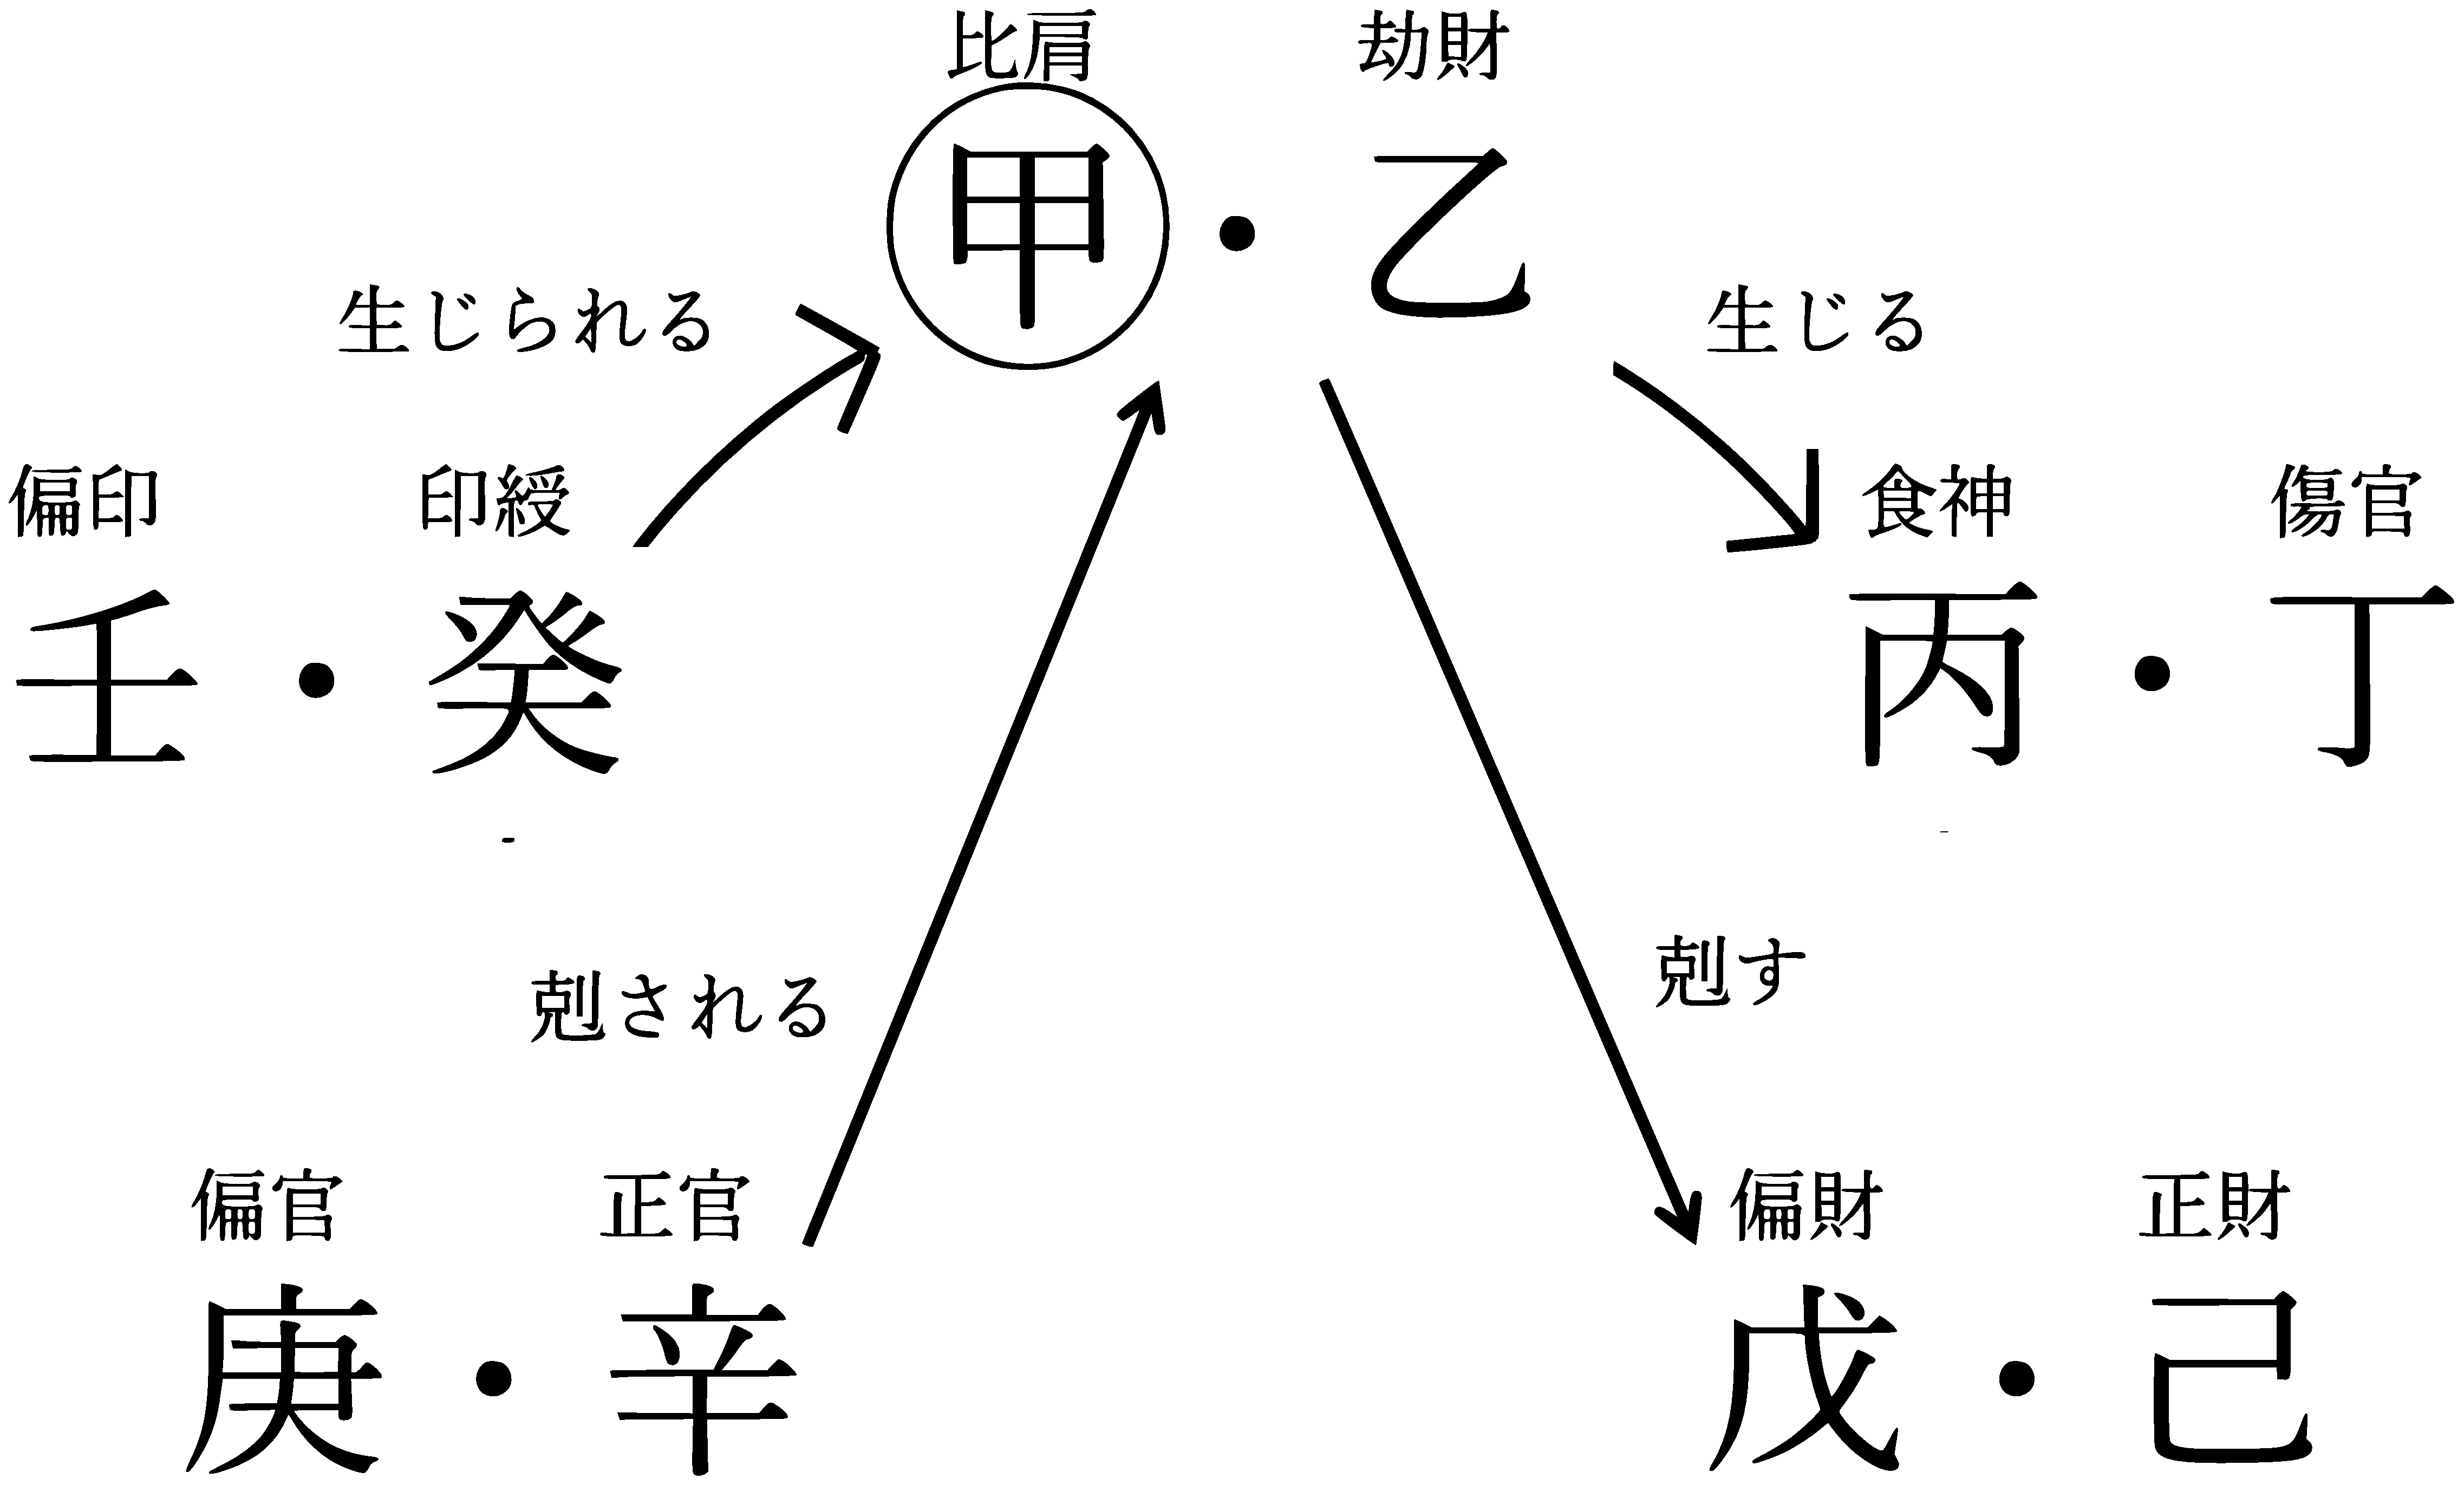
\includegraphics[width=65mm,angle=90]{figs/figure5-4.eps}
\end{wrapfigure}

このように、甲から見て、他の干の陰陽五行を二字熟語(通変)で表現すると、次の十種類にまとめられます。

\begin{itemize}
  \item 陽と陽の\ruby{木生火}{もくしょうか} → 食神
  \item 陽と陰の\ruby{木生火}{もくしょうか} → 傷官
  \item 陽と陽の\ruby{木剋土}{もっこくど} → 偏財
  \item 陽と陰の\ruby{木剋土}{もっこくど} → 正財
  \item 陽と陽の\ruby{金剋木}{きんこくもく} → 偏官
  \item 陽と陰の\ruby{金剋木}{きんこくもく} → 正官
  \item 陽と陽の\ruby{水生木}{すいしょうもく} → 偏印
  \item 陽と陰の\ruby{水生木}{すいしょうもく} → 印綬
  \item 陽と陽の同一五行 → 比肩
  \item 陽と陰の同一五行 → 劫財
\end{itemize}

今度は「癸」を基準にしましょう。この場合に「丙」の通変を考えると、癸(水)にとって丙(火)は「剋す五行」であり(\ruby{水剋火}{すいこくか})、陰陽は「陰」と「陽」で異なります。この場合、丙の通変は「\ruby{正財}{せいざい}」になります。

同様に「辛」を考えると、癸(水)にとって辛(金)は「生じられる五行」であり(\ruby{金生水}{きんしょうすい})、陰陽は「陰」と「陰」で同じです。この場合、辛の通変は「\ruby{偏印}{へんいん}」になります。

さらに「乙」を考えると、癸(水)にとって乙(木)は「生じる五行」であり(\ruby{水生木}{すいしょうもく})、陰陽は「陰」と「陰」で同じです。この場合、乙の通変は「\ruby{食神}{しょくじん}」になります。

\begin{wrapfigure}{l}[0pt]{0.25\textwidth}
  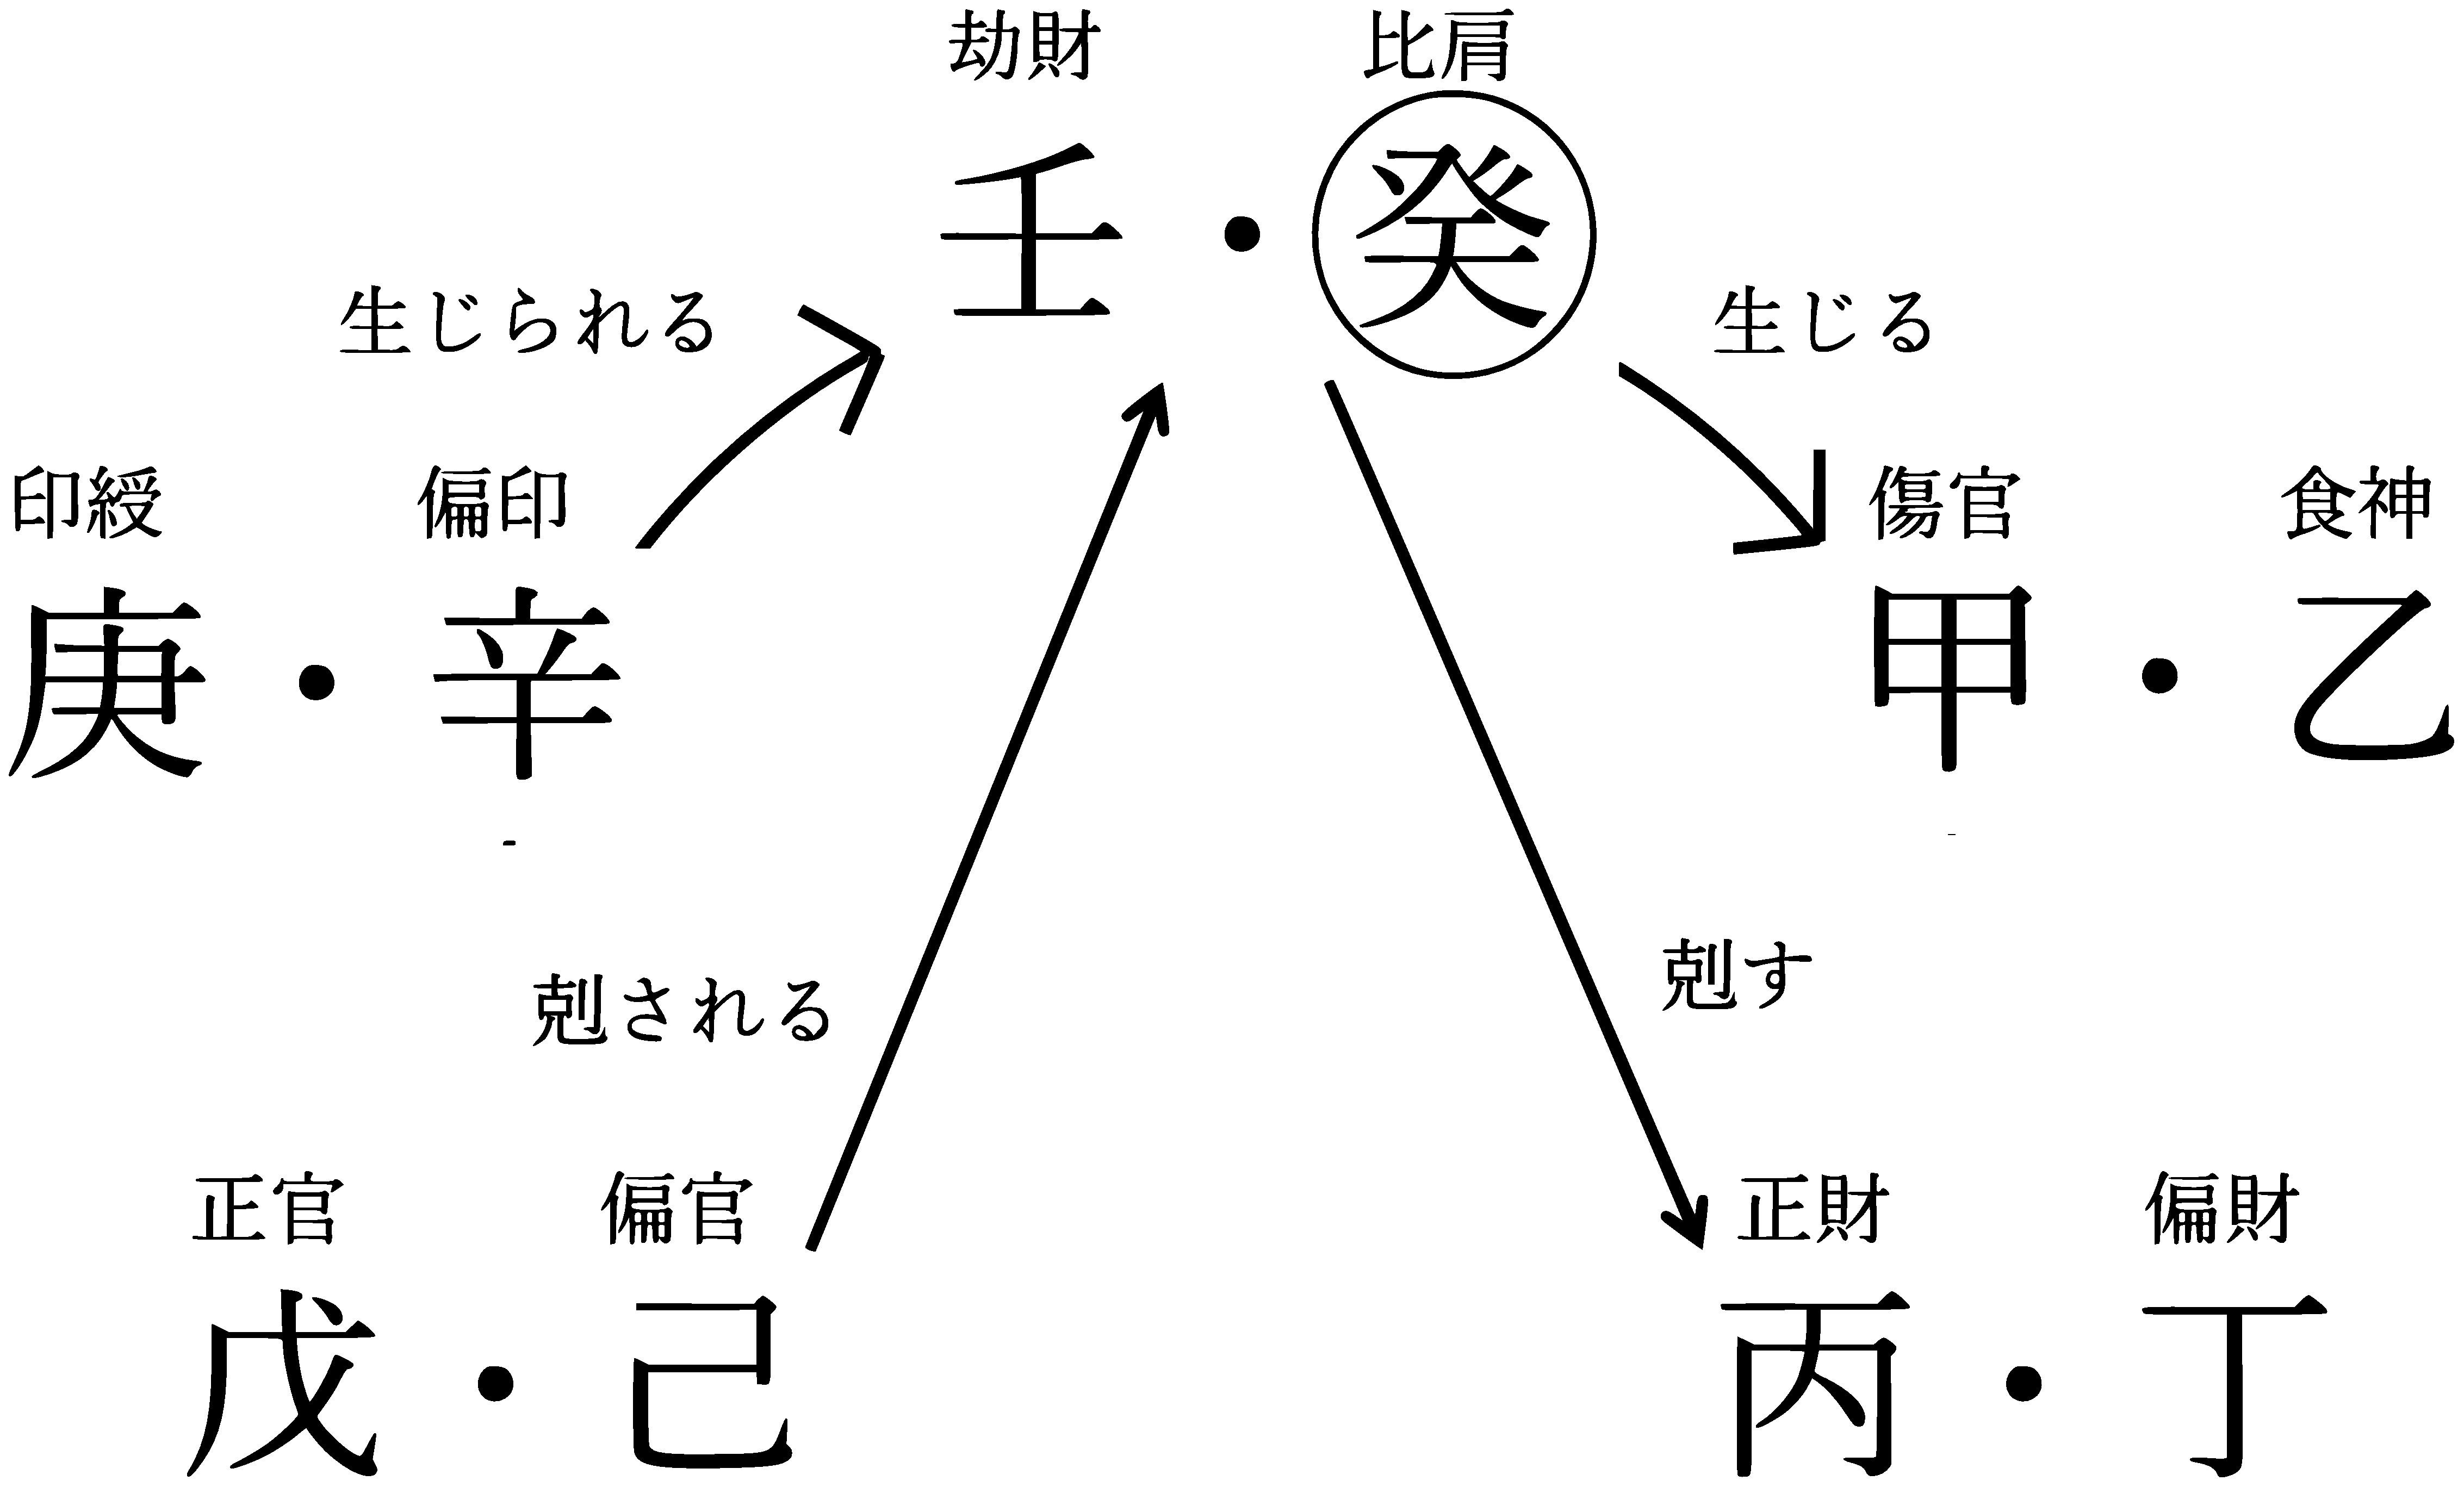
\includegraphics[width=65mm,angle=90]{figs/figure5-5.eps}
\end{wrapfigure}

このように、癸から見て、他の干の陰陽五行を二字熟語(通変)で表現すると、次の十種類にまとめられます。

\begin{itemize}
\item 陰と陰の\ruby{水生木}{すいしょうもく}→食神
\item 陰と陽の\ruby{水生木}{すいしょうもく}→傷官
\item 陰と陰の\ruby{水剋火}{すいこくか}→偏財
\item 陰と陽の\ruby{水剋火}{すいこくか}→正財
\item 陰と陰の\ruby{土剋水}{どこくすい}→偏官
\item 陰と陽の\ruby{土剋水}{どこくすい}→正官
\item 陰と陰の\ruby{金生水}{きんしょうすい}→偏印
\item 陰と陽の\ruby{金生水}{きんしょうすい}→印綬
\item 陰と陰の同一五行→比肩
\item 陰と陽の同一五行→劫財
\end{itemize}

これらの例では「甲」「癸」を基準にして考えましたが、他の干でも同様です。これを一覧表にすると、次のようになります。

\begin{figure}[h]
  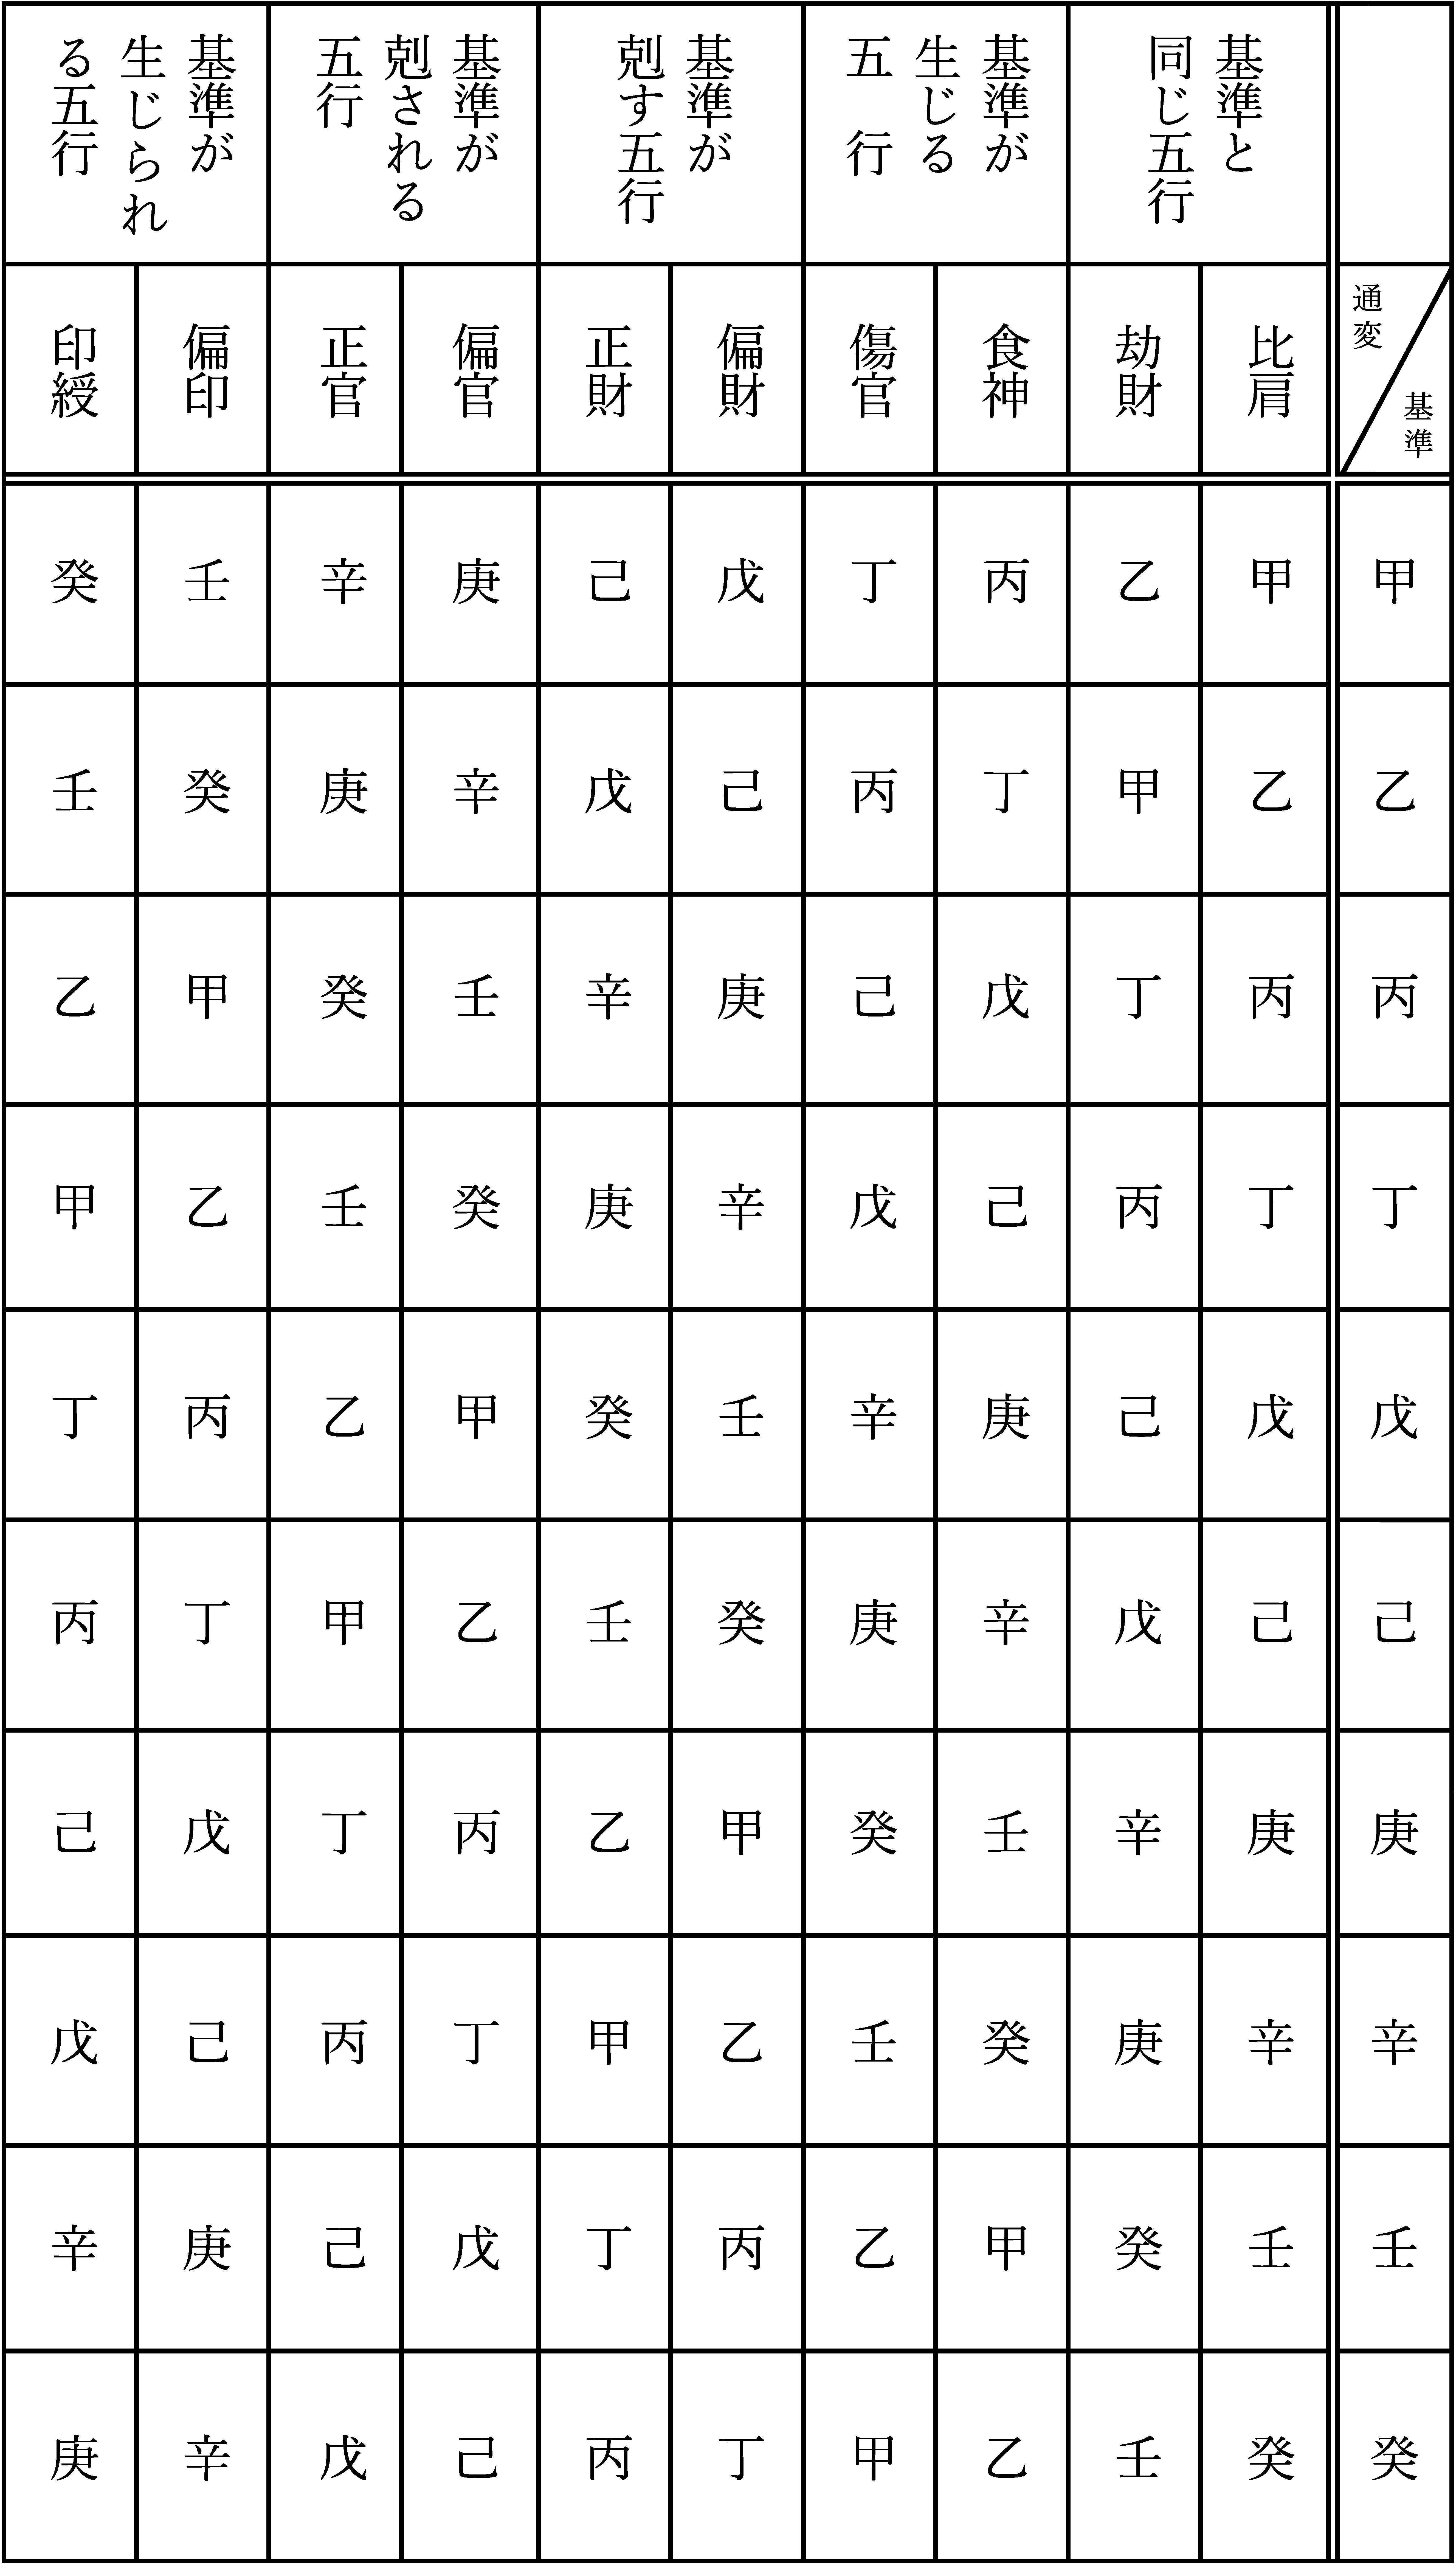
\includegraphics[width=80mm,angle=90]{figs/figure5-6.eps}
\end{figure}

四柱推命学に習熟するためには、この表を見ることなく、二つの干の関係を即座に通変に置き換えられるようにならなければなりません。そのためには、まずは理屈を運用して変換できるようにしましょう。

例えば、「壬」を基準として「己」の通変を考える場合、

\begin{enumerate}
\item 「水」は「土」に剋される(\ruby{土剋水}{どこくすい})
\item 「壬」と「己」は陰陽が異なる
\item 剋される関係にあって陰陽が異なる場合の通変は「\ruby{正官}{せいかん}」である
\end{enumerate}
のように考えます。理屈の運用では変換に時間がかかりますが、次第にすべての組み合わせを記憶できるため、即座に置き換えられるようになります。

\subsection{命式・大運における通変}
命式・大運を導いた後は、それらに含まれる干に対して、日干を基準とした通変をつけます。

例えば、平成\rensuji{13}年\rensuji{10}月\rensuji{18}日\rensuji{17}時0分生まれの女性の命式・大運には、次のように通変がつけられます。\footnote{日干を基準として通変をつけるため、日干自身には通変はつけません。また、日干を基準とする理由は、四柱推命学においては、日干を「自分自身を表す干」と考えるからです。}

\begin{figure}[h]
  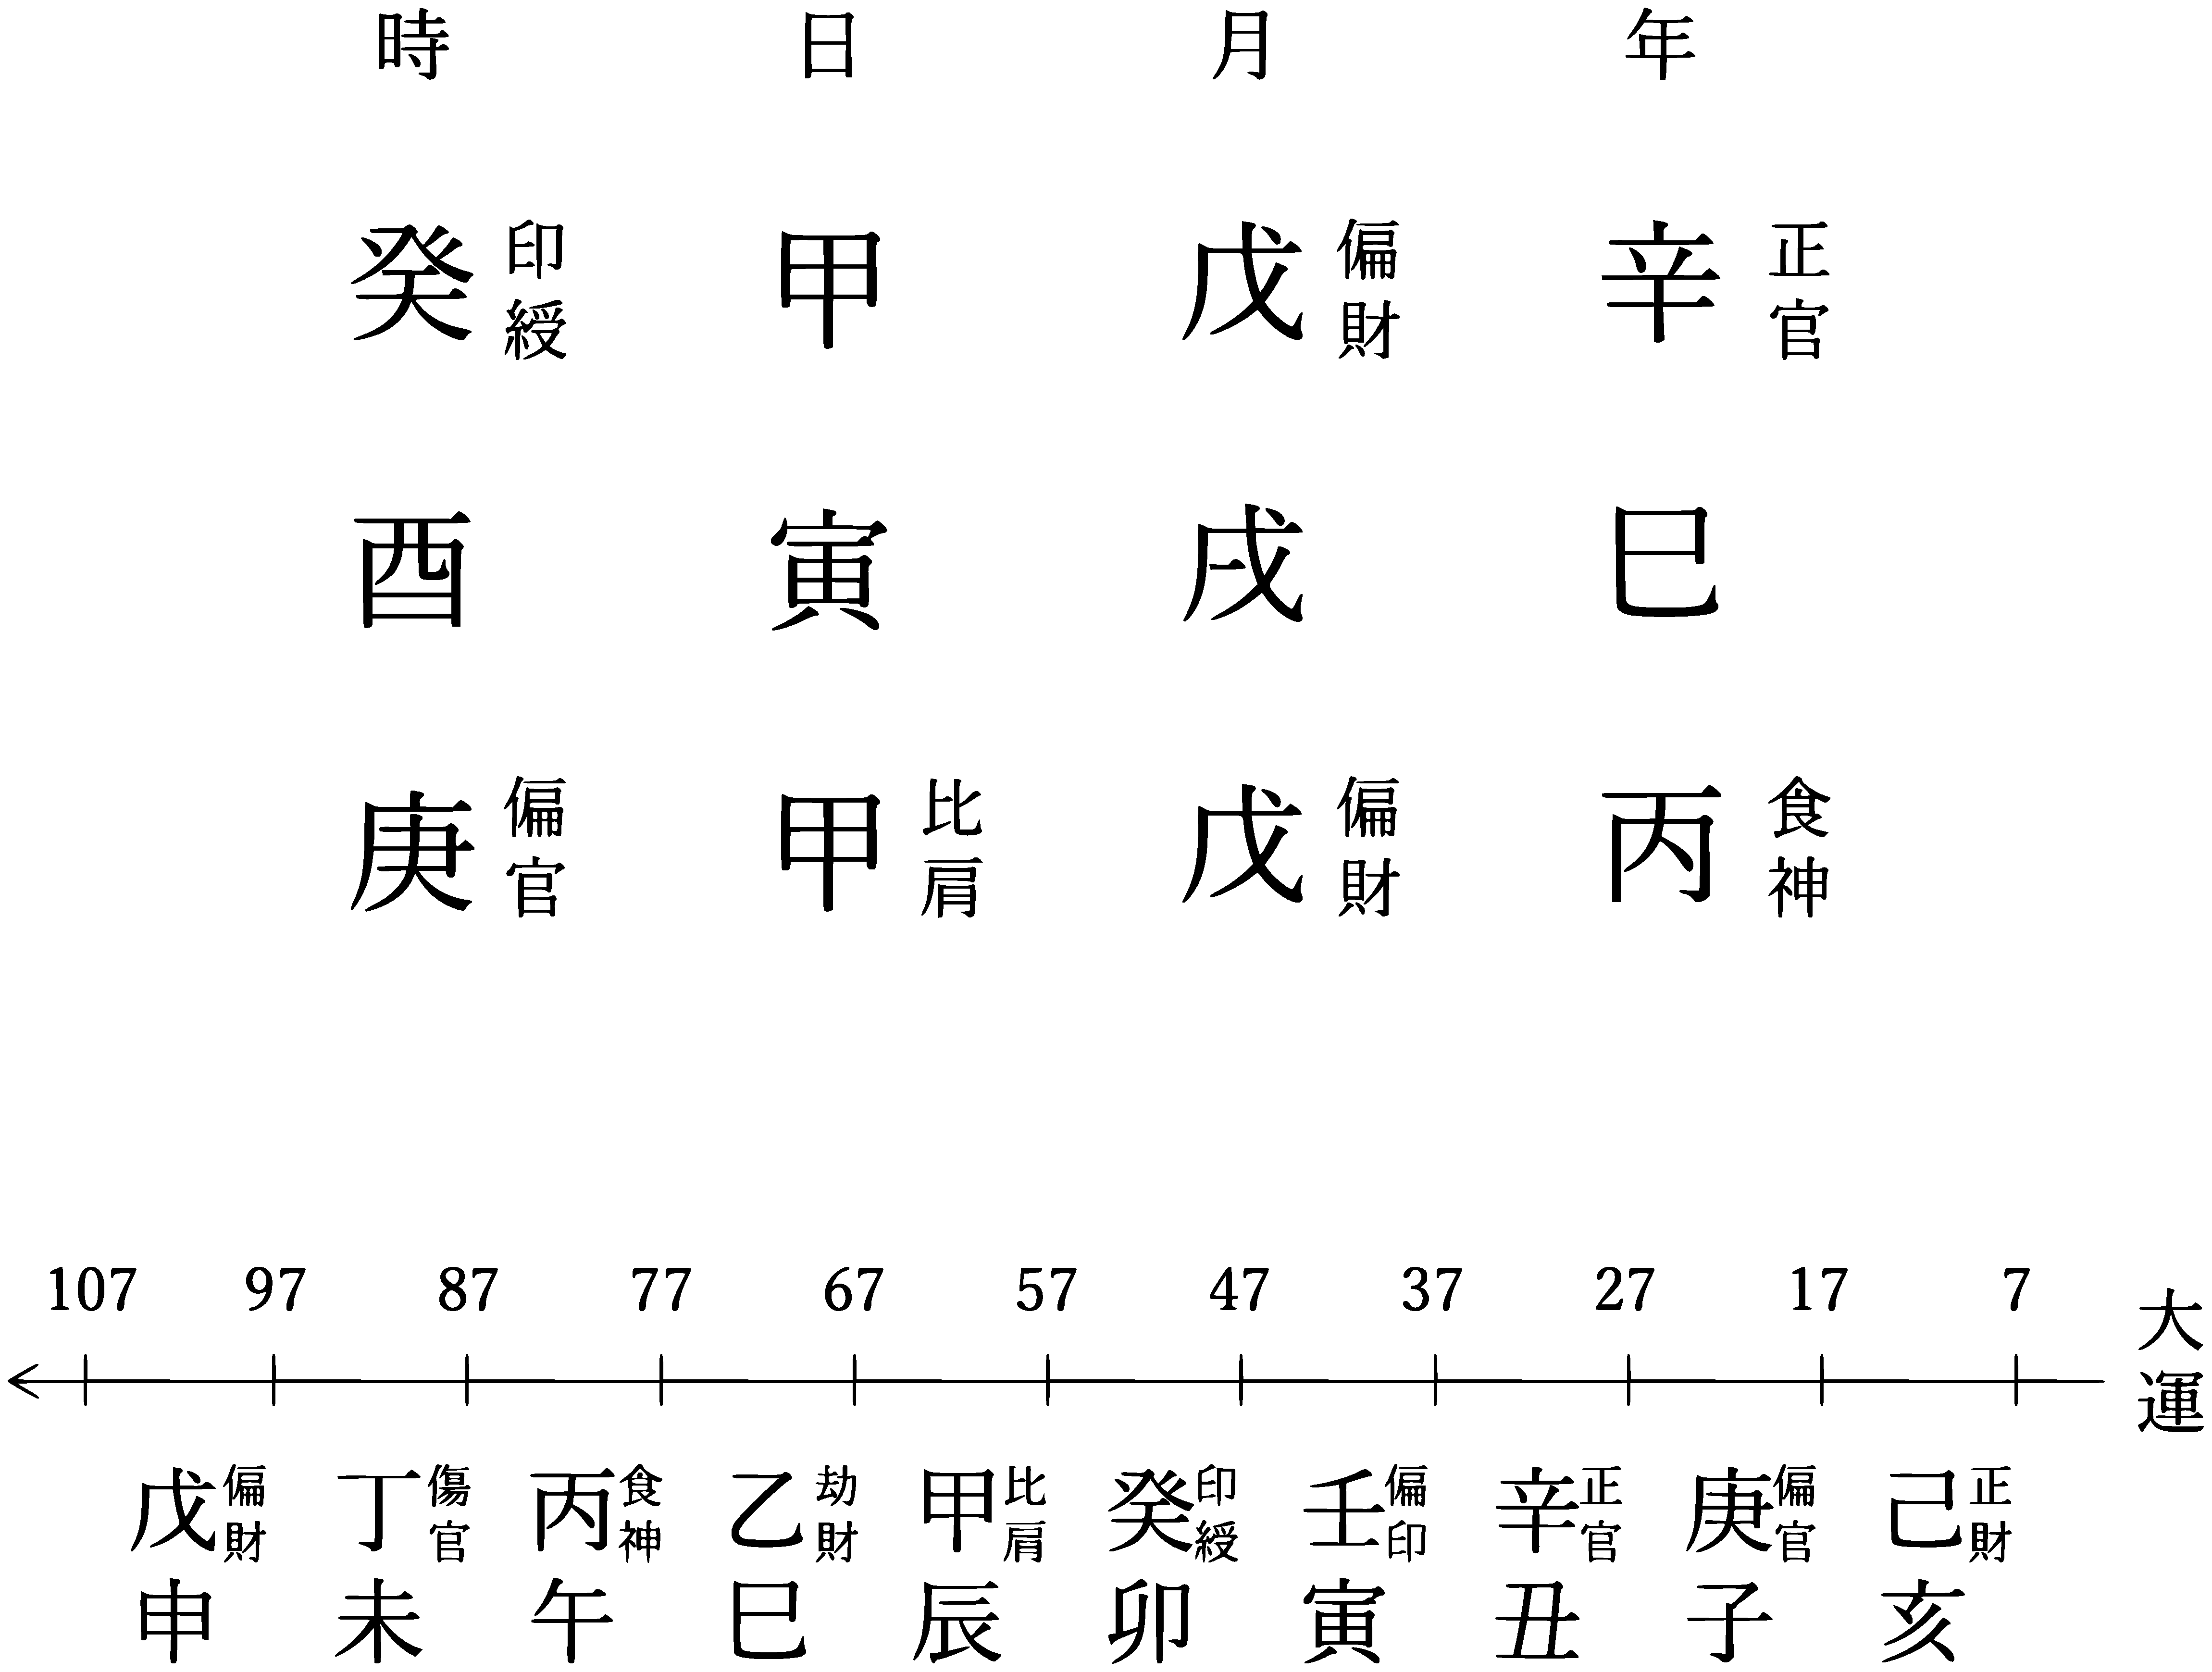
\includegraphics[width=75mm,angle=90]{figs/figure5-7.eps}
\end{figure}

このように、命式・大運に通変をつけた後は、各通変がどのような働きをするかを詳細に分析することで、看命を進めることになります。

\subsection{良い通変と悪い通変}
看命の原則として、良い通変と悪い通変を列挙します。
\begin{description}
\item[良い通変(\ruby{吉神}{きっしん})] \ruby{食神}{しょくじん}・\ruby{偏財}{へんざい}・\ruby{正財}{せいざい}・\ruby{正官}{せいかん}・\ruby{印綬}{いんじゅ}
\item[悪い通変(\ruby{凶神}{きょうじん})] \ruby{比肩}{ひけん}・\ruby{劫財}{ごうざい}・\ruby{傷官}{しょうかん}・\ruby{偏官}{へんかん}・\ruby{偏印}{へんいん}
\end{description}
  
命式・大運に良い通変が多くあれば運が良く、悪い通変が多くあれば運が悪いという単純な話ではありません。命式の状態によっては、悪い通変が大運・年運に巡ることを喜ぶ場合もありますし、逆に、良い通変が巡ることを嫌う場合もあります。例えば、命式において日干が弱い場合は、良い通変である「\ruby{正官}{せいかん}」を嫌い、悪い通変である「\ruby{偏印}{へんいん}」を喜ぶことがあります。\footnote{通変による強弱については、第六章参照。}

ここでは、一応の原則として、良い通変と悪い通変の分類を覚えておきましょう。

\subsection{月支蔵干通変(用神・格)}

原則として、月支蔵干の通変を\ruby{用神}{ようじん}といいます。先の例では、月支蔵干「戊」の通変は「\ruby{偏財}{へんざい}」ですから、この\ruby{偏財}{へんざい}が用神となります。

用神が決まると、その命式の\ruby{格}{かく}が決まります。先の例では、用神が「\ruby{偏財}{へんざい}」ですから、この命式の格は「\ruby{偏財格}{へんざいかく}」となります。格は、\ruby{食神格}{しょくじんかく}、\ruby{傷官格}{しょうかんかく}、\ruby{偏財格}{へんざいかく}、\ruby{正財格}{せいざいかく}、\ruby{偏官格}{へんかんかく}、\ruby{正官格}{せいかんかく}、\ruby{偏印格}{へんいんかく}、\ruby{印綬格}{いんじゅかく}と、八種類あります。そして、日干と格との均衡・不均衡を検討することが、看命の基本となります。\\

ここで、均衡・不均衡を理解するために、四柱命式の全体を一つの「会社」と考えてみましょう。まず、日干は私自身であり、会社を代表する「社長」です。一方、用神は会社のナンバー2である「専務」です。

社長の力が強すぎて専務が腰巾着になり、会社がワンマン運営になると、その会社の未来は暗いでしょう。逆に、社長が頼りなくて専務の勝手が過ぎても、やはり暗いでしょう。社長と専務は同じくらいの存在感で均衡しており、互いに手を取り合って会社の発展に尽くすのが望ましいのです。四柱命式においては、日干と格とがバランス(均衡)していることが重要です。

うまくバランスしていない場合は、大運・年運による作用でバランスが取れることを喜びます。例えば、日干が強すぎて命式が「ワンマン会社」になっている場合は、日干の力が衰え、格の力が増す時期を喜びと考えます。逆に、日干が弱すぎて命式が「リーダーシップ不在の会社」になっている場合は、日干の力が増す時期を喜びと考えます。また、バランスしている場合であっても、大運・年運による作用でそれが崩れる時期は要注意です。

陰陽説では、自然界の全てのものを「陰」と「陽」の相反する二つの要素で相対的にとらえます。そして、これらが互いに消長し、調和することによって自然界の秩序が保たれていると解釈するのでした。\footnote{第二章参照}

四柱推命学では、命式における「日干」と「格」という二つの要素を相対的にとらえます。そして、「均衡の原則」にしたがって、日干と格とが均衡(調和)していることを喜びます。そのため、日干と格との力関係を測ることが看命の基本となります。\\

なお、月支蔵干通変が「\ruby{比肩}{ひけん}」または「\ruby{劫財}{ごうざい}」の場合は、これらを格とすることはできません。先に「原則として」と述べ、格は「八種類」と説明したのはこれが理由です(「\ruby{比肩格}{ひけんかく}」「\ruby{劫財格}{ごうざいかく}」は存在しません)。

月支蔵干通変が「\ruby{比肩}{ひけん}」または「\ruby{劫財}{ごうざい}」の場合、まずは時柱天干通変を参照します。そして、その通変が「良い通変」である場合はそれを格とします。

例えば、次の命式を考えます。

\begin{figure}[h]
  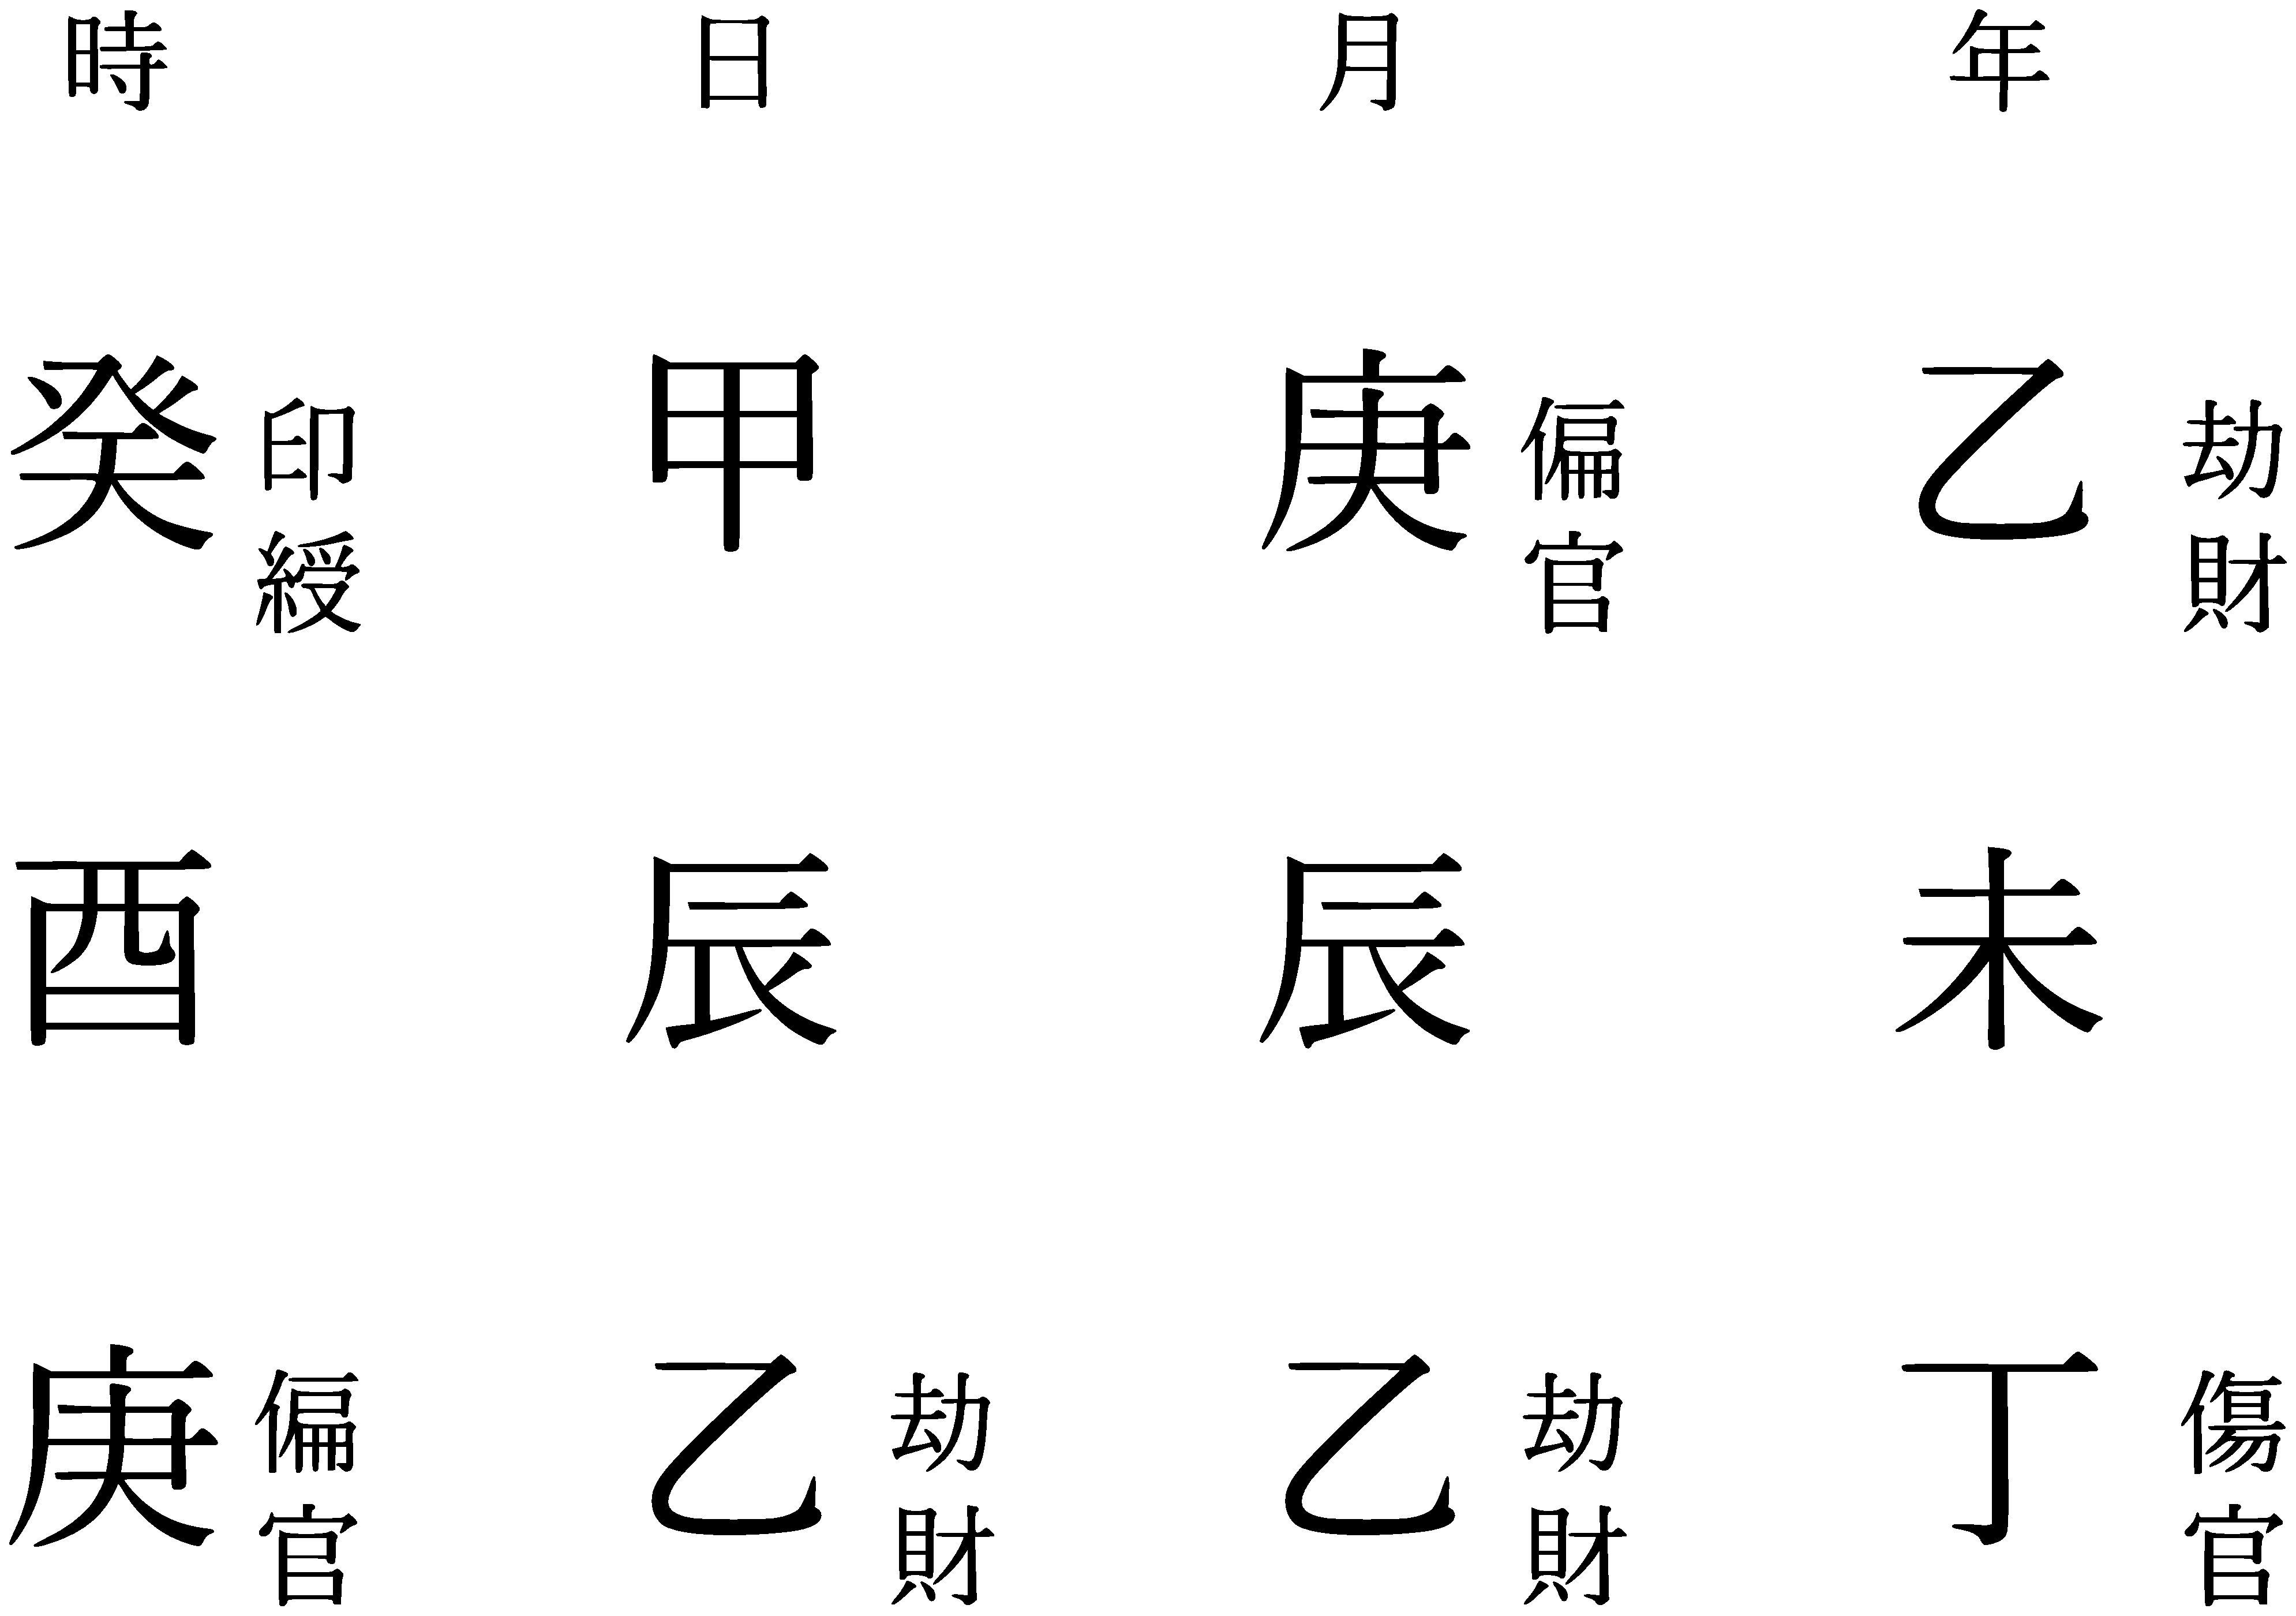
\includegraphics[width=60mm,angle=90]{figs/figure5-8.eps}
\end{figure}

この命式の場合、月支蔵干の通変は「\ruby{劫財}{ごうざい}」であるため、これを格とすることはできません。そのため、時柱天干にあって良い通変である「\ruby{印綬}{いんじゅ}」を格とします。この命式の格は「\ruby{印綬格}{いんじゅかく}」です。

時柱天干通変でも格をとれない場合(時柱天干通変も\ruby{比肩}{ひけん}・\ruby{劫財}{ごうざい}である場合、または、時柱天干通変が悪い通変である場合)、次は年柱天干通変を参照し、その通変が「良い通変」である場合はそれを格とします。

さらに、年柱天干通変でも格をとれない場合は時柱蔵干通変を参照し、それでも格をとれない場合は年柱蔵干通変を参照します。

このように、月支蔵干通変が「\ruby{比肩}{ひけん}」または「\ruby{劫財}{ごうざい}」の場合は、格のとりかたが変則的になるので注意が必要です。



\clearpage

\section{旺衰強弱}

日干と格との均衡・不均衡を検討することが看命の基本であることを、先に述べました。そのためには、日干・用神の\ruby{旺衰強弱}{おうすいきょうじゃく}をそれぞれ測る必要があります。

旺衰強弱を測る方法は、四つあります。

\begin{enumerate}
\item \ruby{月令}{げつれい}
\item 十二運
  \item 通変による作用
\item 干・支の変化による作用
\item 大運・年運による作用
\end{enumerate}

これらを順番に説明しましょう。

\subsection{月令}
\ruby{月令}{げつれい}は、干の旺衰を測る一つの指標です。命式が構成されると、日干の五行(木火土金水)が分かります。そこで、
\begin{enumerate}
\item 日干の五行と同じ季節に生まれている
\item 日干の五行を生じてくれる季節に生まれている
\end{enumerate}
のいずれかの条件を満たす場合、「月令を得ている」といい、日干は盛んであるとひとまず推定します。逆に、条件を満たさない場合は「月令を得ず」といい、日干は衰えているとまずは推定します。

これと同じ要領で、用神の月令もみます。例えば、日干・用神ともに月令を得ている場合は、双方盛んで均衡が取れていると、この時点では推定できます。\\

いくつかの命式を例にして説明します。

\begin{figure}[h]
  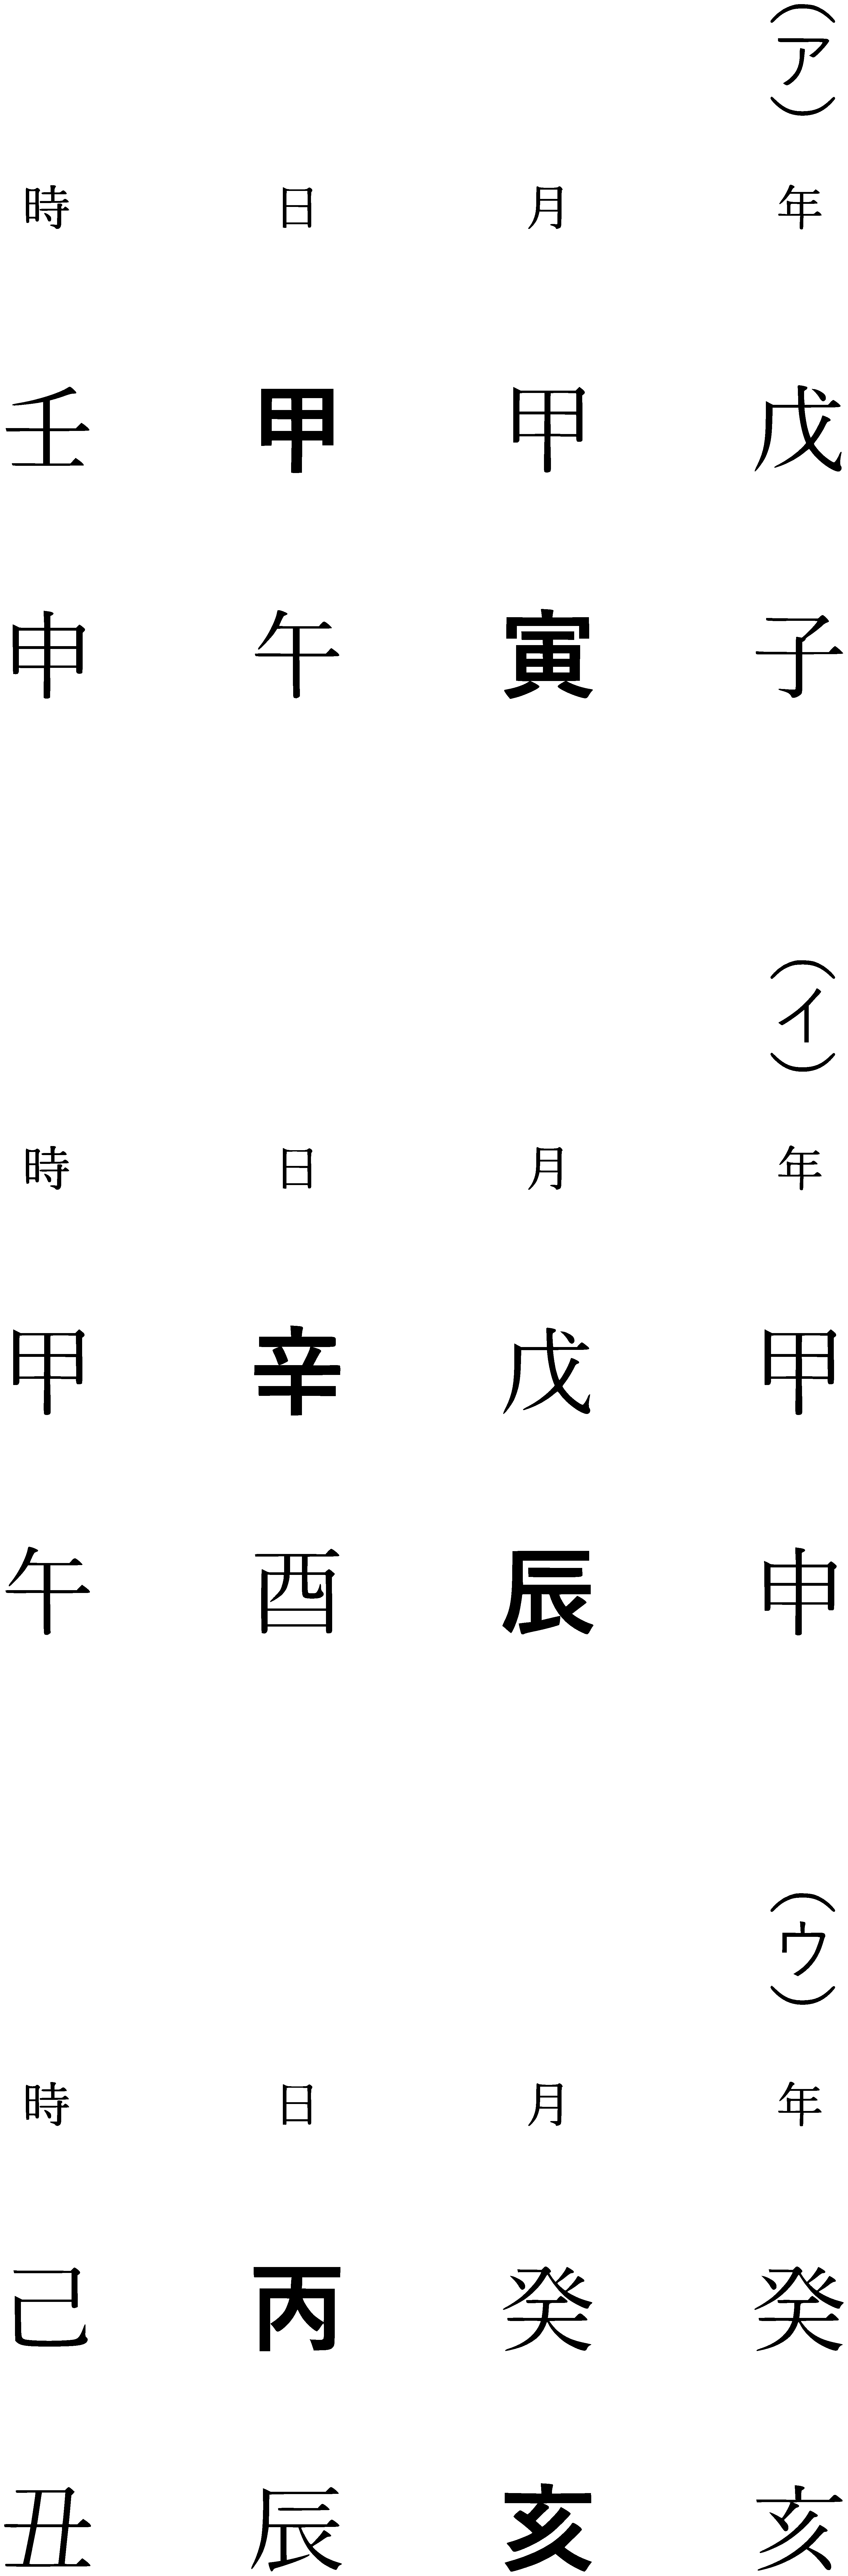
\includegraphics[width=45mm,angle=90]{figs/figure6-1.eps}
\end{figure}

日干は「甲」ですから、その五行は「木」です。一方で、月支(生まれた月)は「寅」であり、その季節は「春」(木の季節)です。五行と季節が一致しますので、条件1を満たし、日干は「月令を得ている」と分かります。

一方、用神は「戊」ですから、その五行は「土」です。この場合は、条件1および2のいずれも満たしませんので、用神は「月令を得ず」と分かります。

そのため、月令だけを参酌すれば、日干対格のバランスは崩れている(日干に力が偏っている)と分かります。

\begin{figure}[h]
  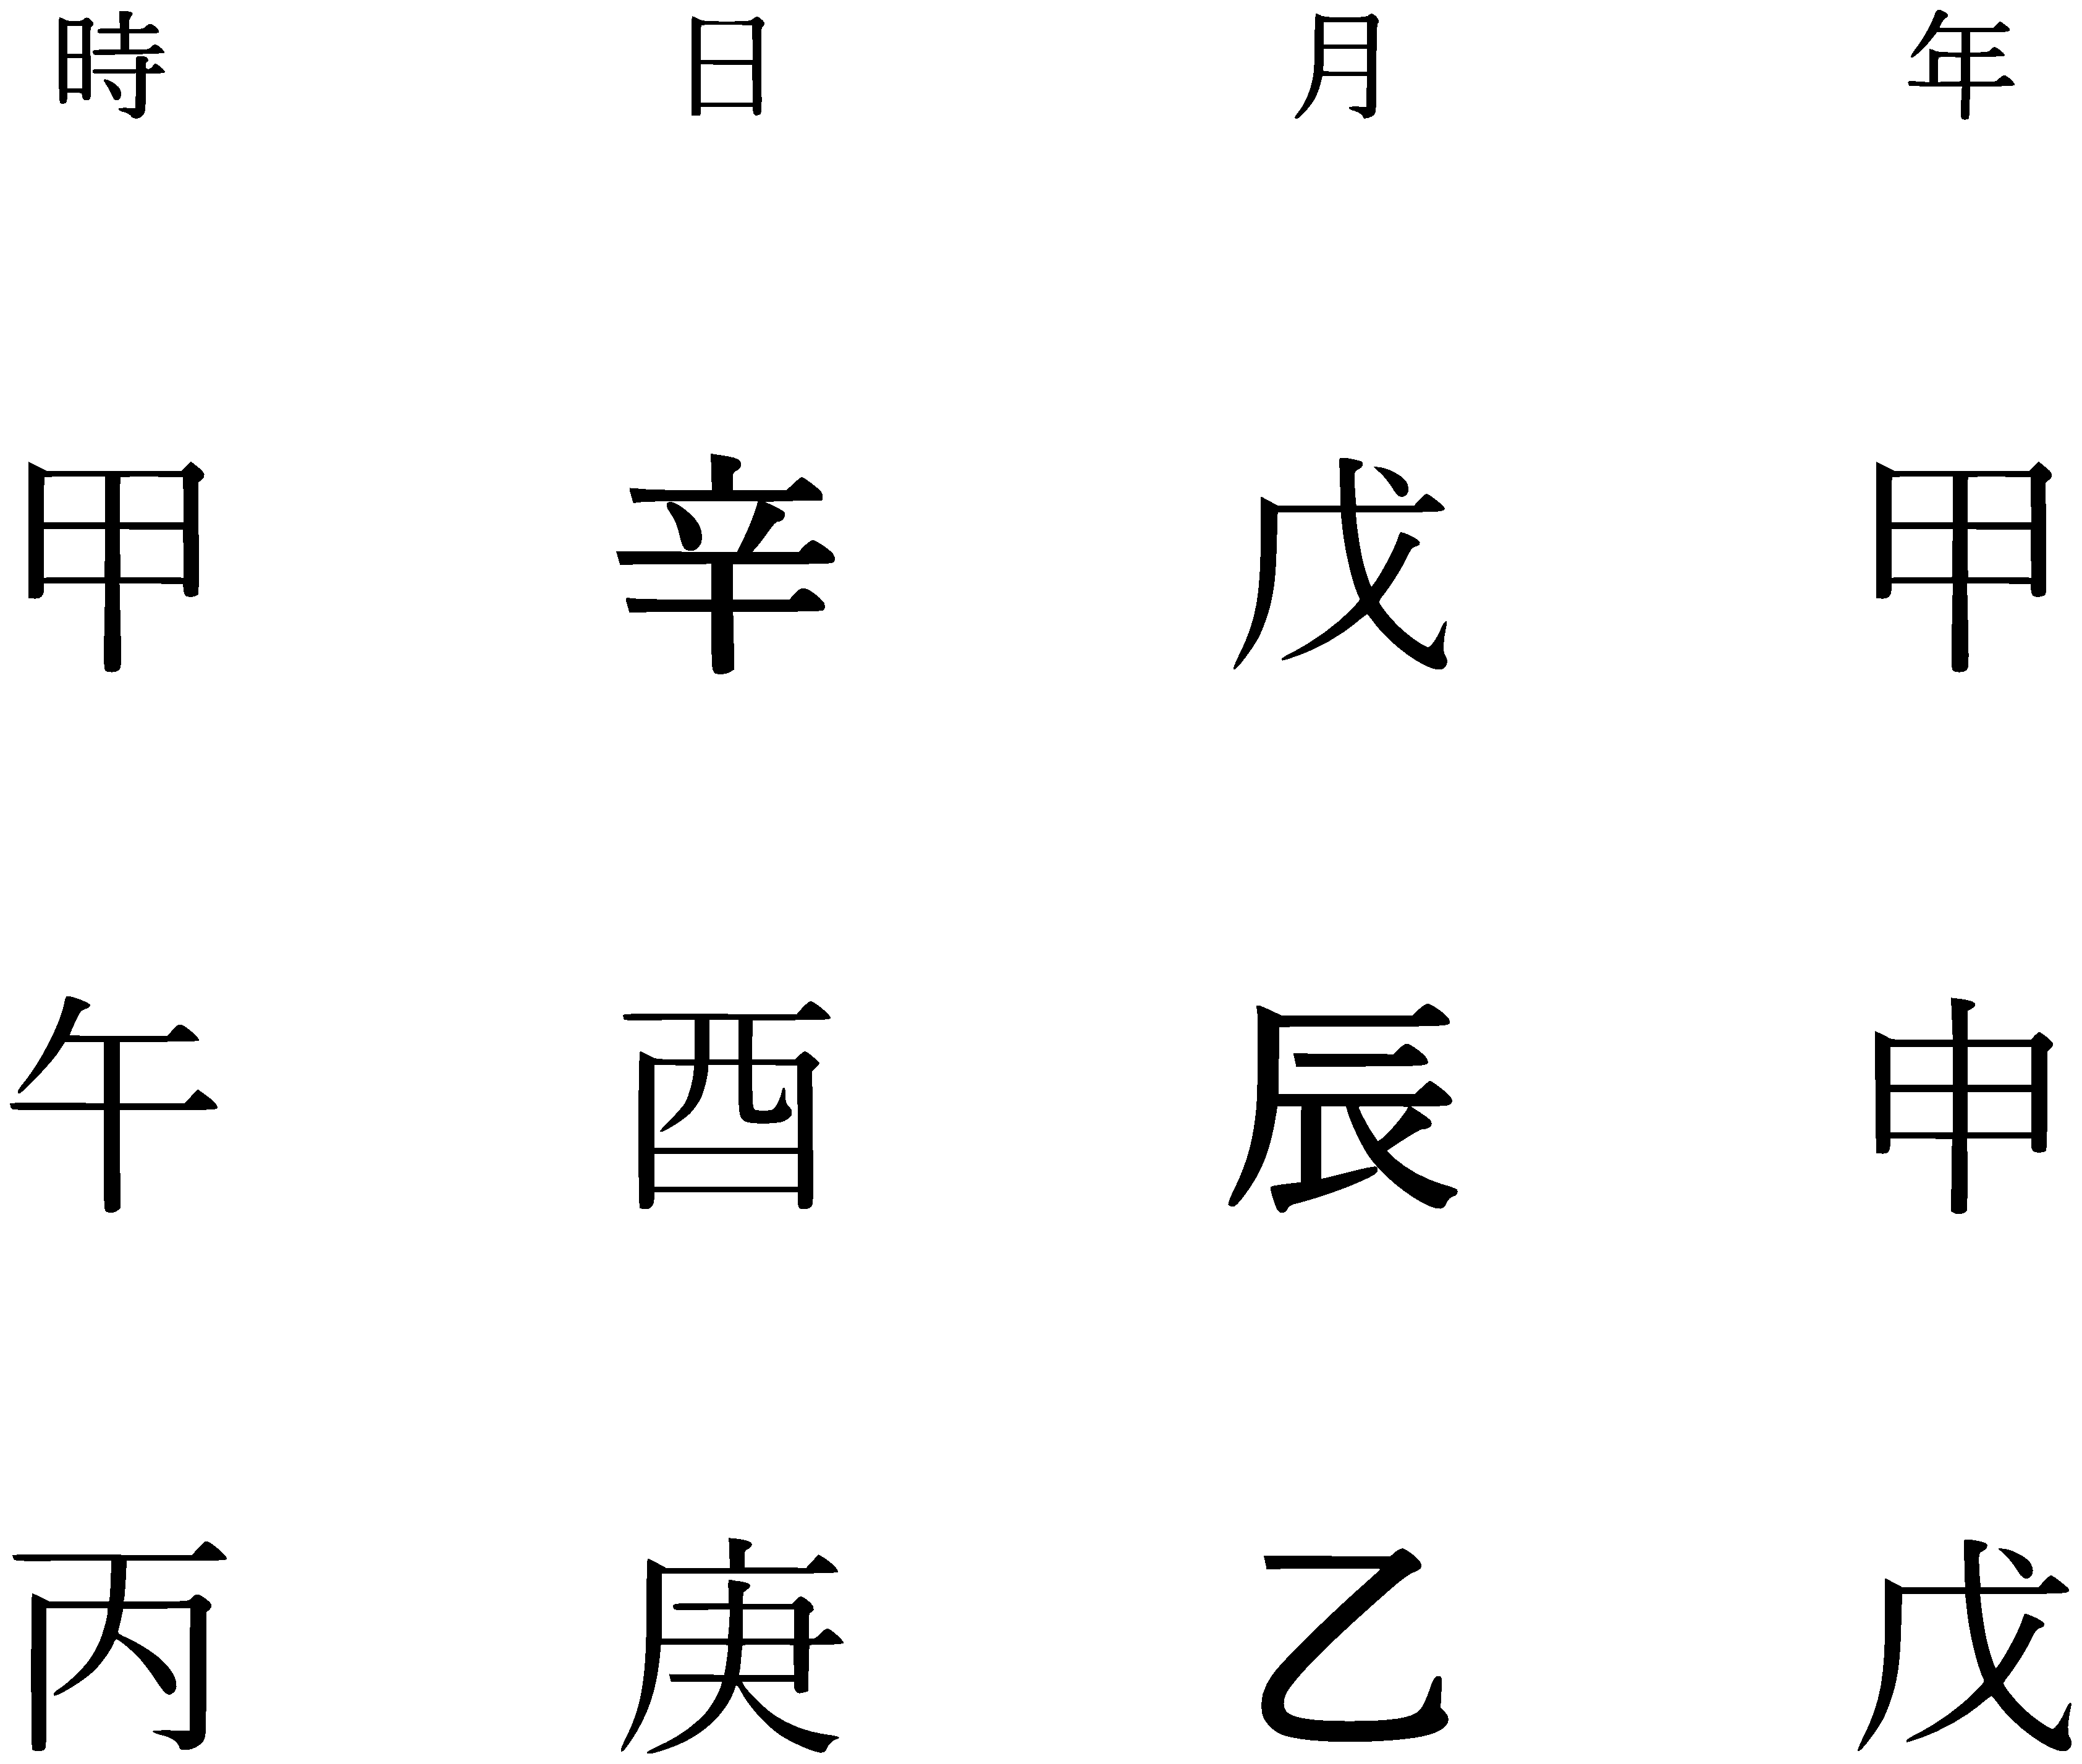
\includegraphics[width=45mm,angle=90]{figs/figure6-2.eps}
\end{figure}

日干は「辛」ですから、その五行は「金」です。一方で、月支は「辰」であり、その季節は「土用」(土の季節)です。金は土に生じられる(\ruby{土生金}{どしょうきん})関係にあるので、条件2を満たし、「月令を得ている」と分かります。

一方、用神は「乙」ですから、その五行は「木」です。「辰」の季節は「土用」ですが、それと同時に「春」(木の土)でもあります。そのため、条件1を満たし、用神は「月令を得ている」と分かります。

ここで、辰・未・戌・丑が、それぞれ春・夏・秋・冬を兼ねることに注意が必要です。つまり、辰は「春・土用」(木の土)、未は「夏・土用」(火の土)、戌は「秋・土用」(金の土)、丑は「冬・土用」(水の土)であり、例えば、辰は「土用」であると同時に「春」なのです。

このように、月令を考える場合、辰・未・戌・丑の季節が変則的になるので注意しましょう。

\begin{figure}[h]
  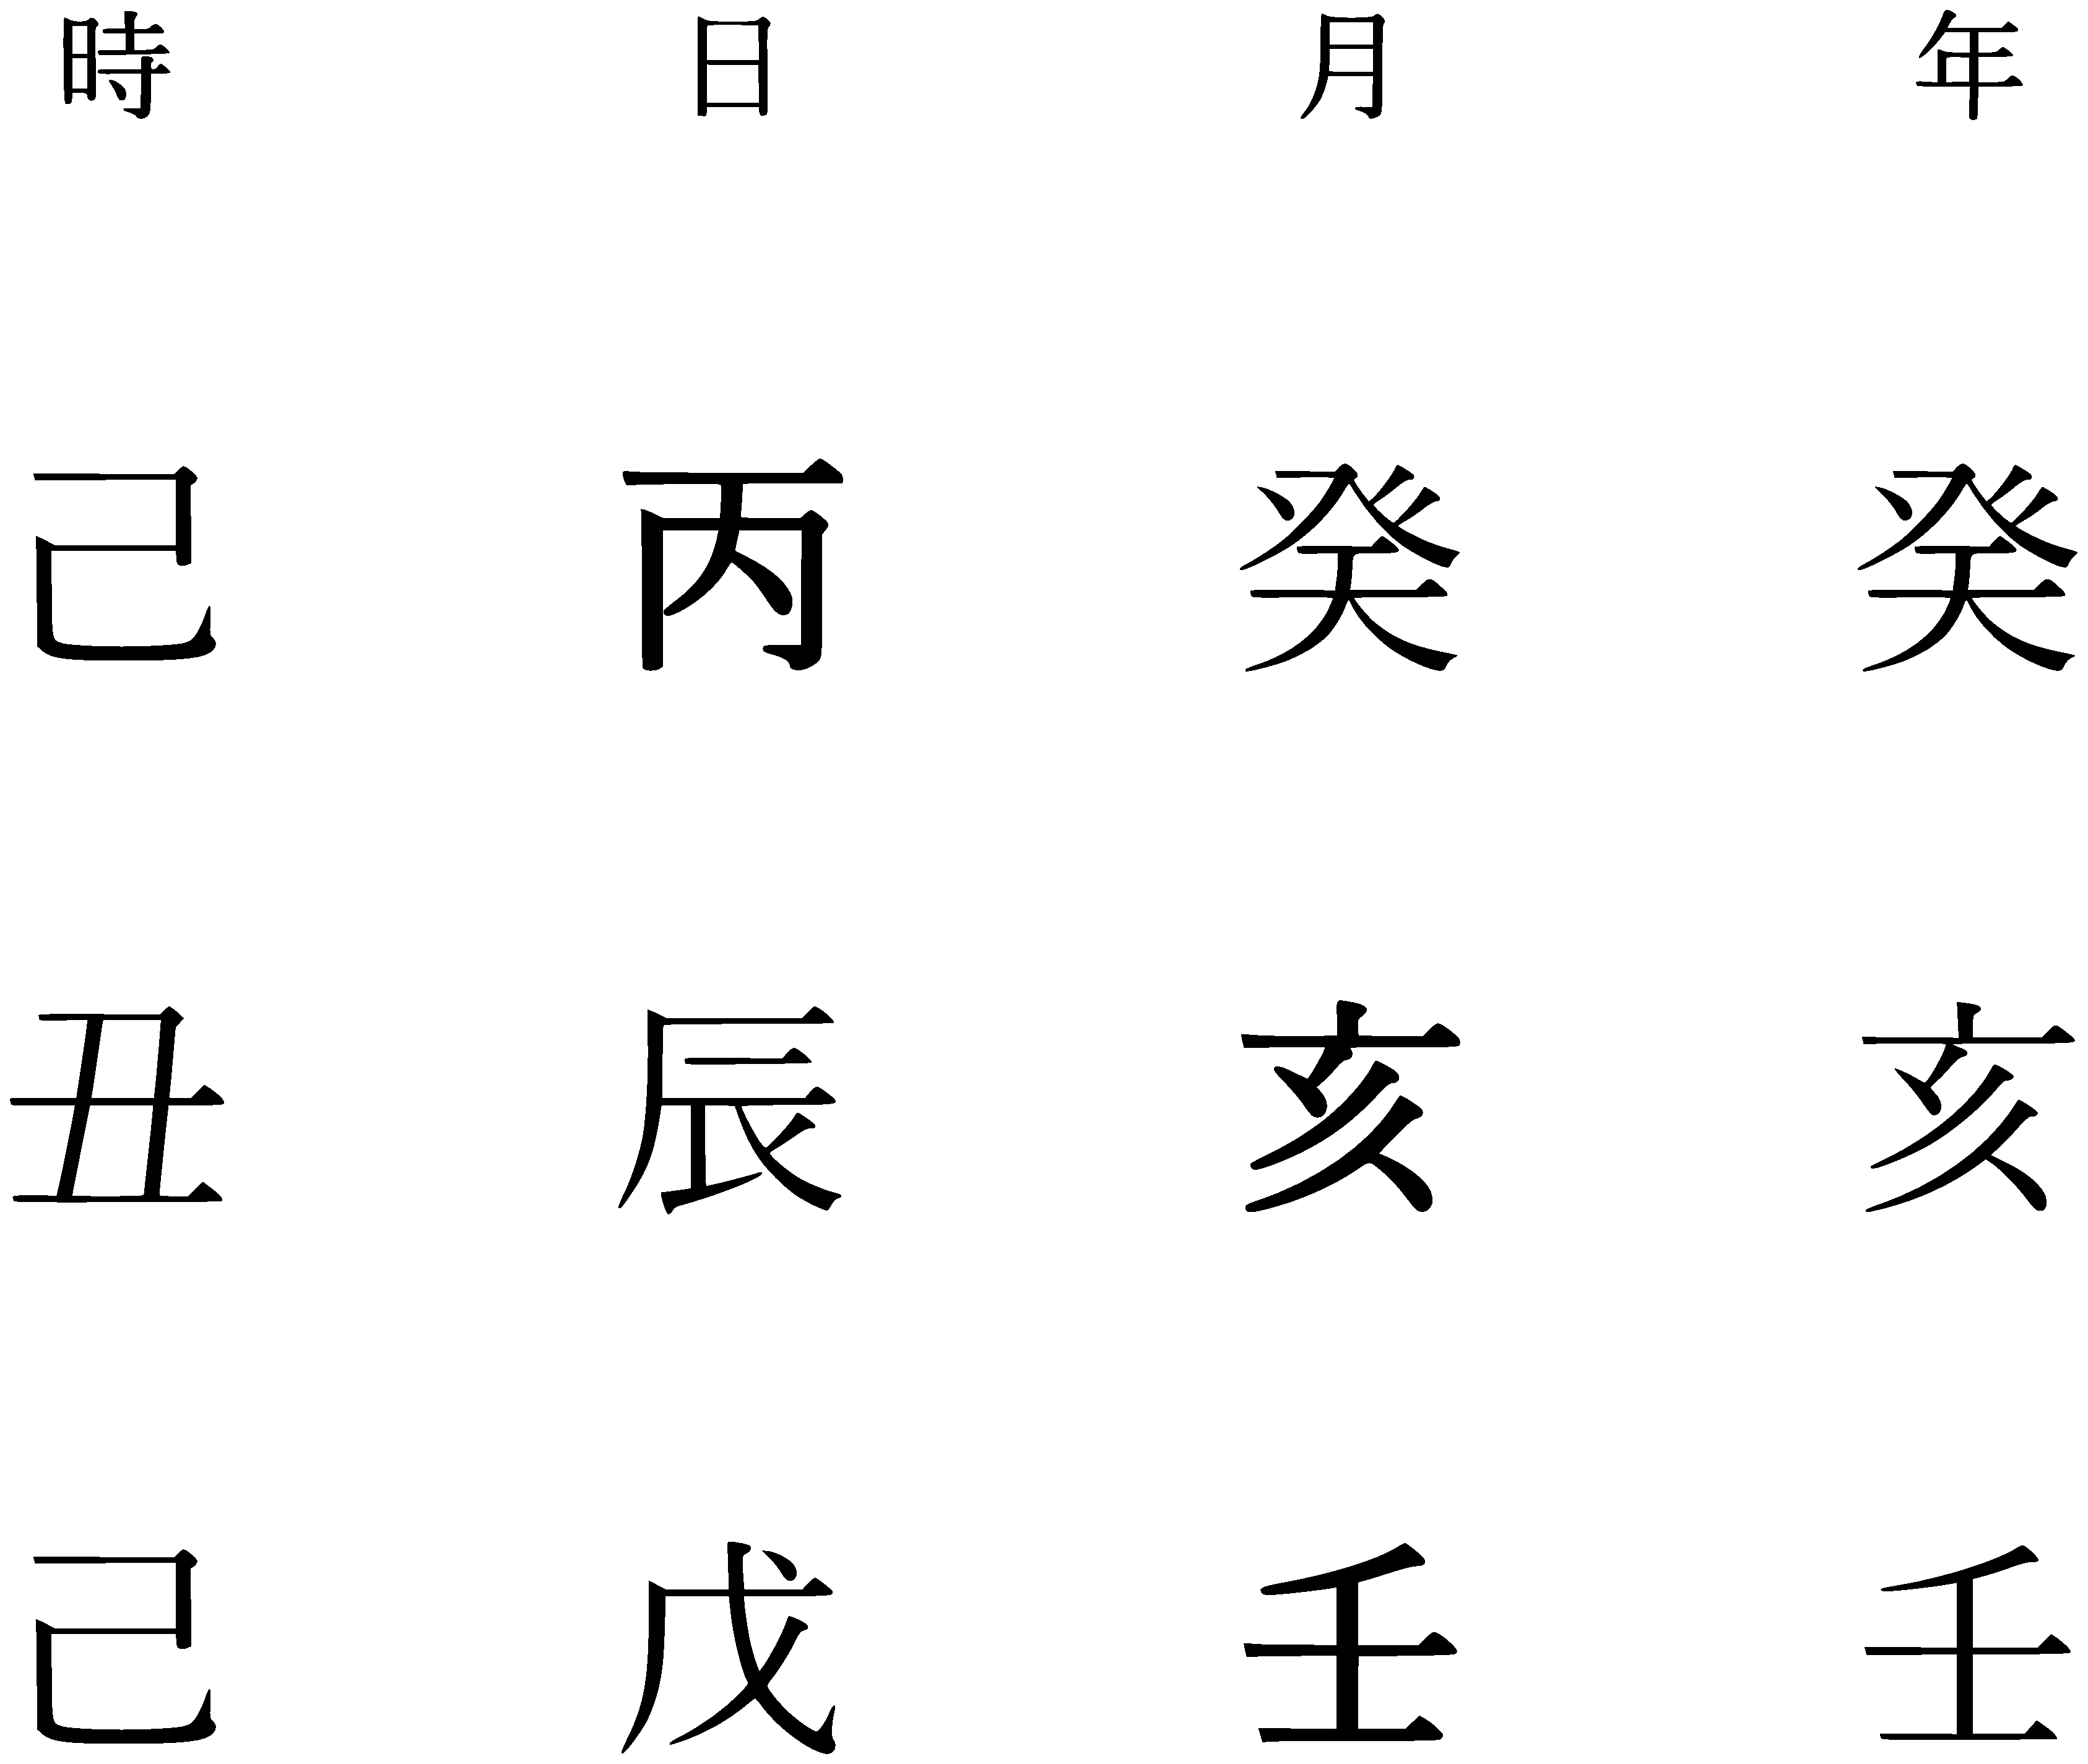
\includegraphics[width=45mm,angle=90]{figs/figure6-3.eps}
\end{figure}

日干は「丙」ですから、その五行は「火」です。一方で、月支は「亥」であり、その季節は「冬」(水の季節)です。この場合は、条件1および2のいずれも満たしませんので、「月令を得ず」と分かります。

一方、用神は「壬」ですから、その五行は「水」です。五行と季節が一致しますので、条件1を満たし、用神は「月令を得ている」と分かります。

月令をまとめると、次の表になります。

【表6−1】

\subsection{十二運}
十二運(補運)とは、日干・用神を基準として地支の強さを測る指標です。つまり、日干・用神から「年・月・日・時」の四つの支に照らし合わせて、どの支が強いか、どの支が弱いかを判定した上で、日干・用神がそれぞれどの程度の強さがあるかを推定するものです。

十二運には、次の十二種類の分類があります。

\begin{enumerate}
\item \ruby{長生}{ちょうせい}:人間が元気よく誕生した状態(強)
\item \ruby{沐浴}{もくよく}:誕生した後で産湯を使っている状態(小強)
\item \ruby{冠帯}{かんたい}:成人式を迎えて元気はつらつとしている状態(強)
\item \ruby{建禄}{けんろく}:中堅として実力を発揮し、活躍している状態(強)
\item \ruby{帝旺}{ていおう}:成功の最頂上にいる状態(強)
\item \ruby{衰}{すい}:やや身体が衰えてきた状態(弱)
\item \ruby{病}{びょう}:病床にある状態(弱)
\item \ruby{死}{し}:逝去の状態(弱)
\item \ruby{墓}{ぼ}:墓石の奥深くに骨を埋められた状態(弱)
\item \ruby{絶}{ぜつ}:骨・魂ともに絶無となる状態(弱)
\item \ruby{胎}{たい}:母胎に生命が宿る状態(小強)
\item \ruby{養}{よう}:胎内で発育し、誕生を待つ状態(小強)
\end{enumerate}

十二運をまとめると、次の表になります。

【表6−2】

いくつかの命式を例にして説明します。

\begin{figure}[h]
  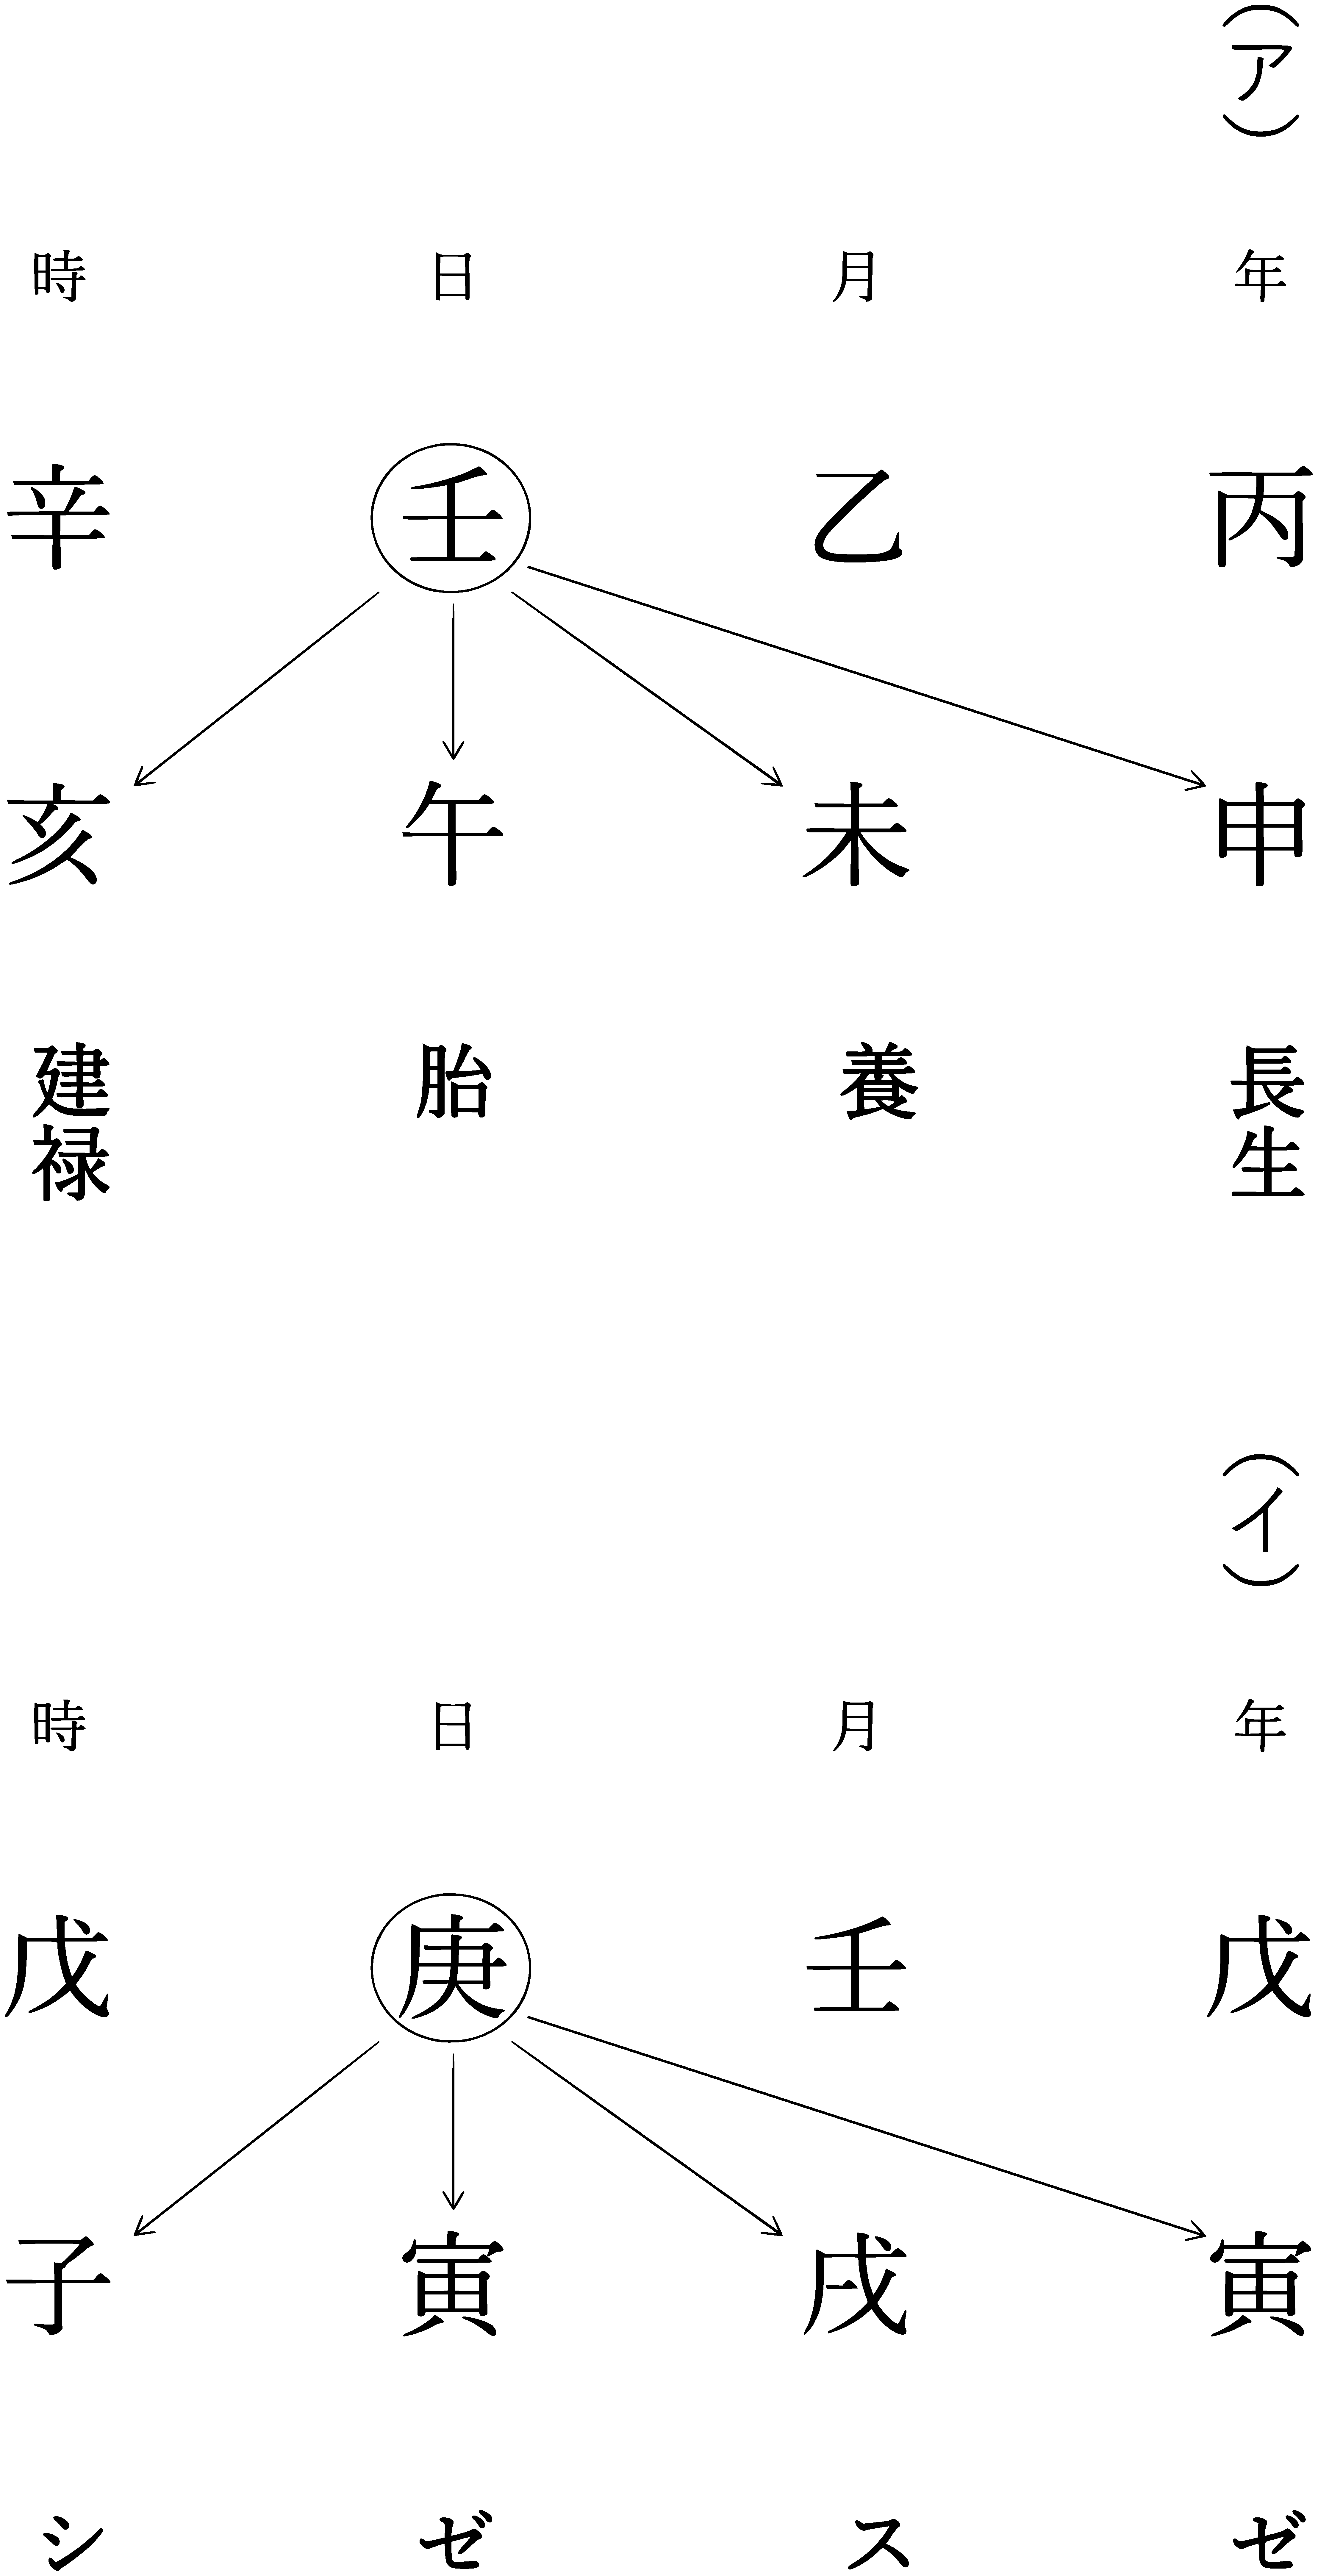
\includegraphics[width=60mm,angle=90]{figs/figure6-4.eps}
\end{figure}

まず、日干は壬ですので、十二運表の「壬」の列で「支」を参照し、そこから横にたどって「十二運」を特定します。すると「申」は「長生(強)」、「未」は「養(小強)」、「午」は「胎(小強)」、「亥」は「建禄(強)」であるため、日干の十二運はかなり強いことが分かります。

次に、用神に対応する月支蔵干は己ですので、「己」の列で「支」を参照し、そこから横にたどって「十二運」を特定します。すると「申」は「沐浴(小強)」、「未」は「冠帯(強)」、「午」は「建禄(強)」、「亥」は「胎(小強)」であるため、用神の十二運もかなり強いことが分かります。

そのため、日干も用神も強い十二運に支えられて、旺じていると判断できます。

\begin{figure}[h]
  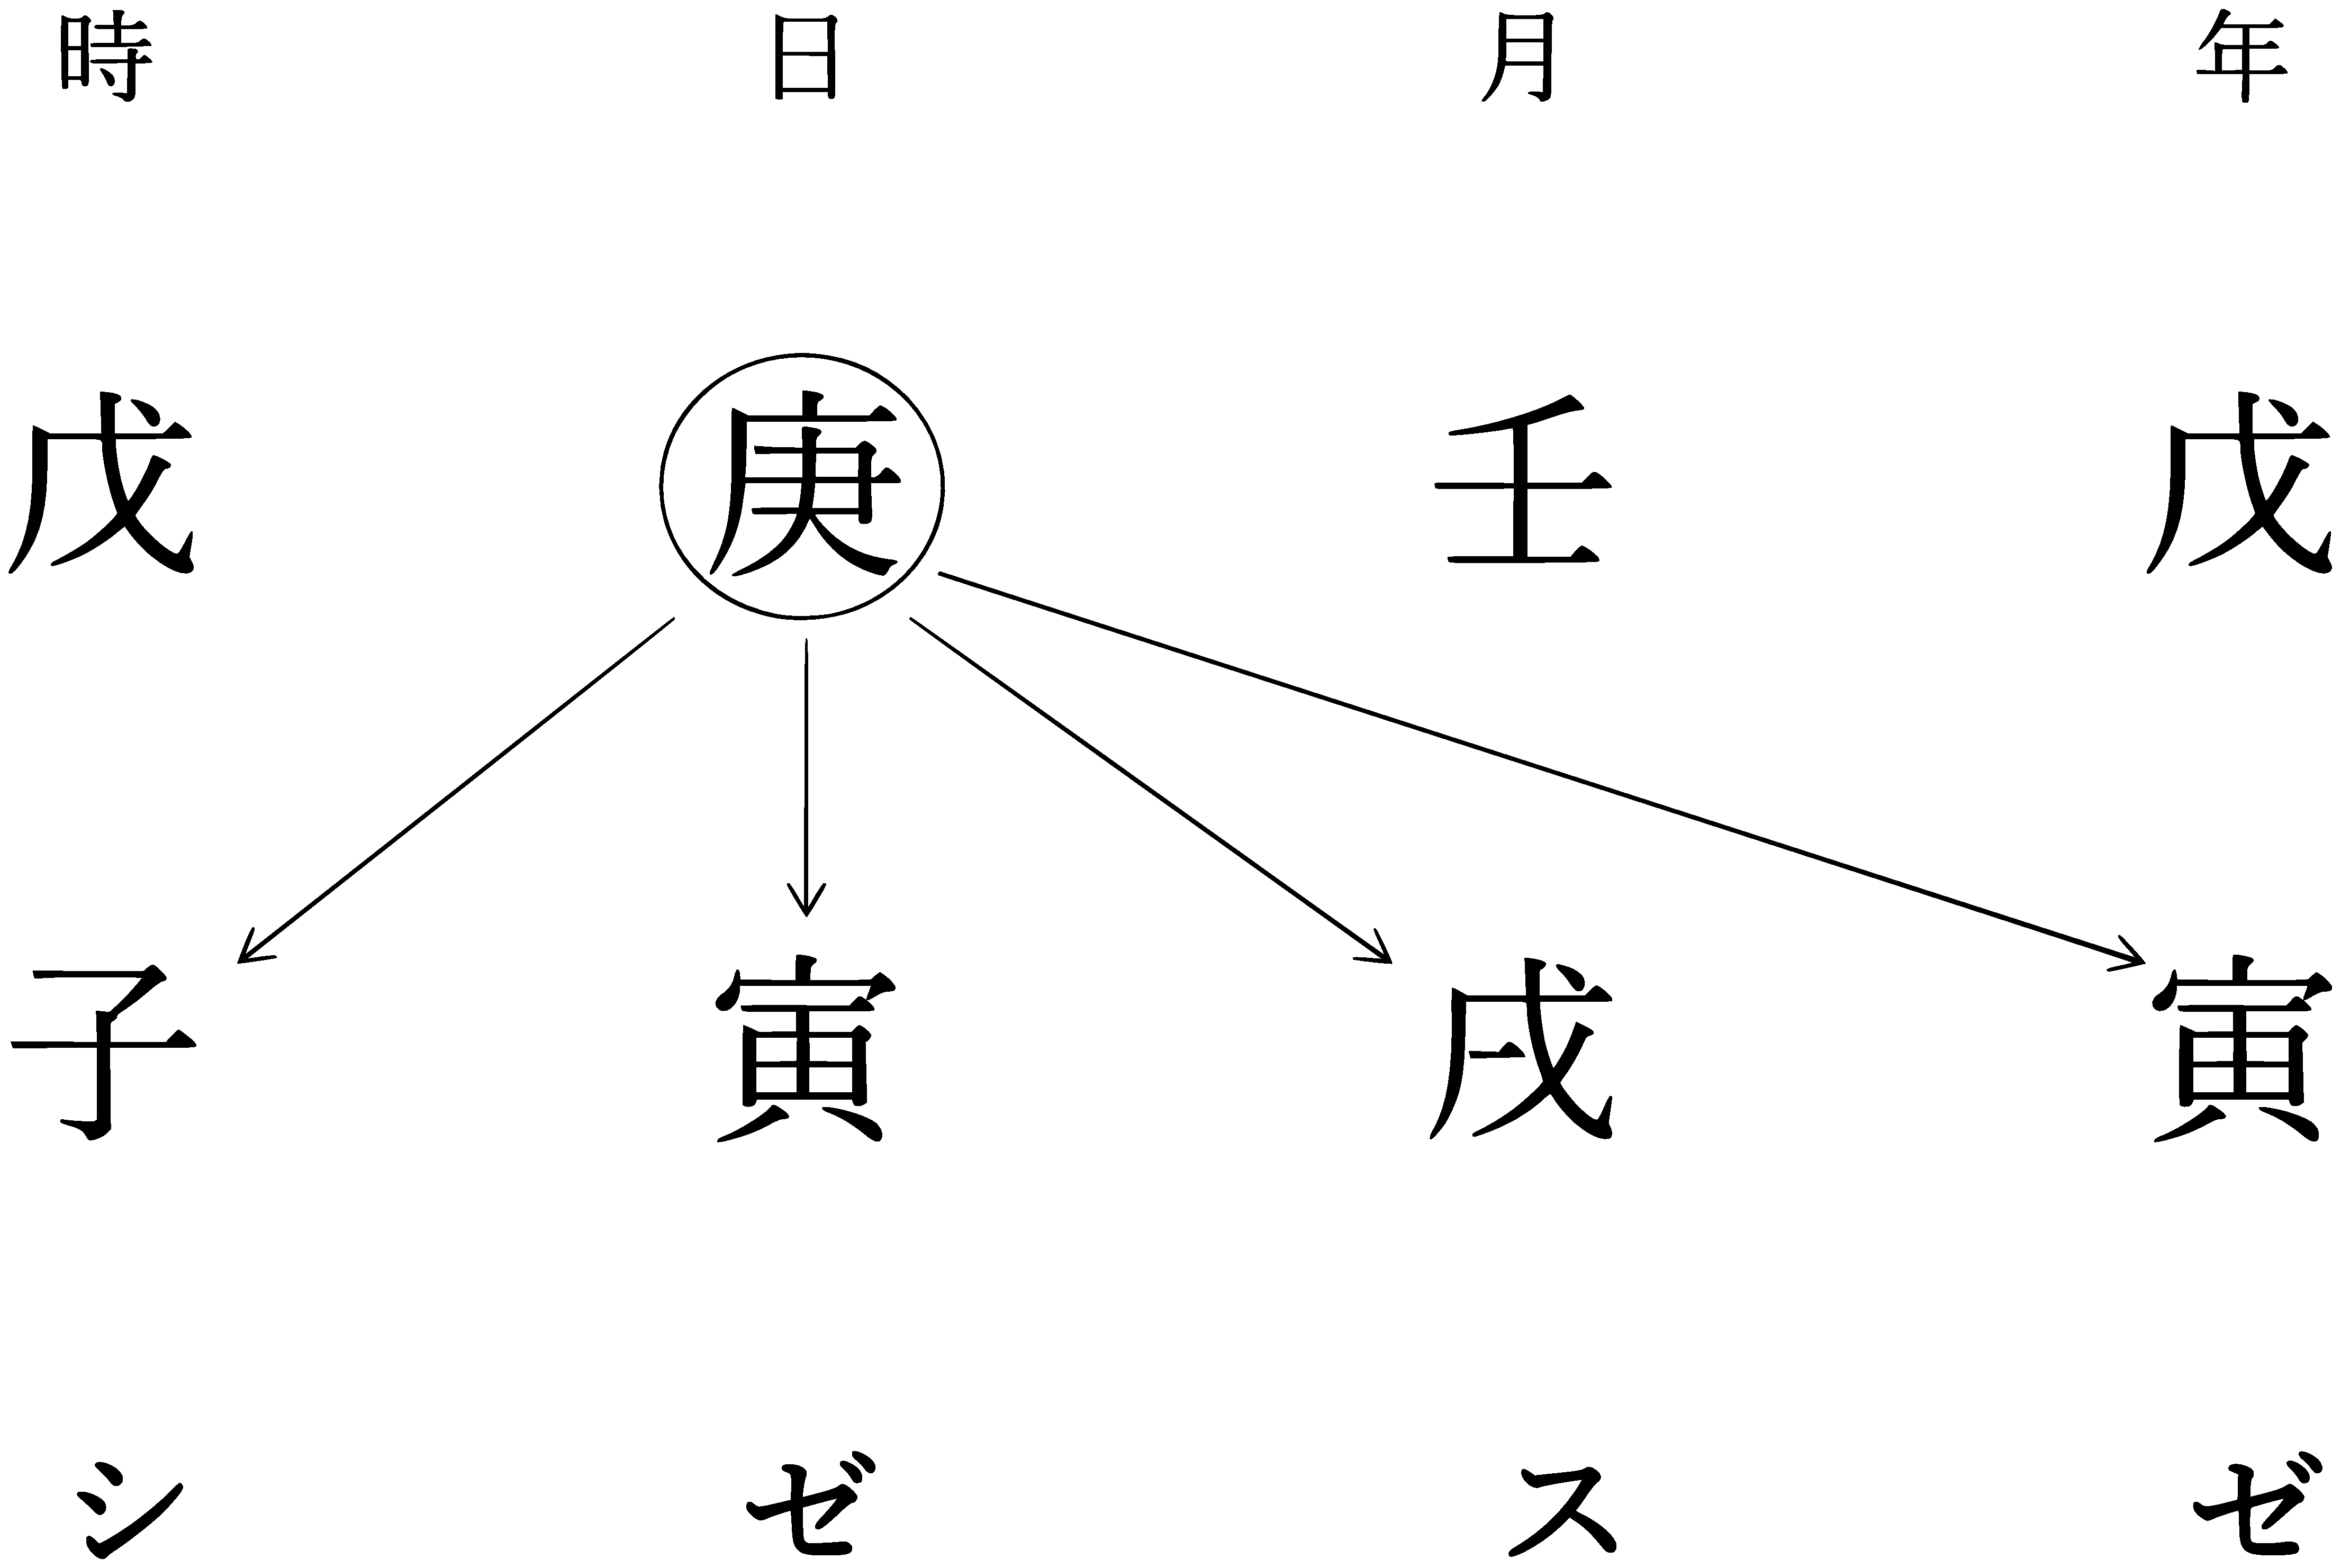
\includegraphics[width=60mm,angle=90]{figs/figure6-5.eps}
\end{figure}

まず、日干は庚ですので、十二運表の「庚」の列で「支」を参照し、そこから横にたどって「十二運」を特定します。すると「寅」は「絶(弱)」、「戌」は「衰(弱)」、「寅」は「絶(弱)」、「子」は「死(弱)」であるため、日干の十二運はかなり弱いことが分かります。

なお、衰・病・死・墓・絶の五つは、漢字から受ける印象が悪いため、それぞれス・ビ・シ・ボ・ゼとカタカナで表記した方がよいでしょう。

次に、用神に対応する月支蔵干は戊ですので、「戊」の列で「支」を参照し、そこから横にたどって「十二運」を特定します。すると「寅」は「長生(強)」、「戌」は「衰(弱)」、「寅」は「長生(強)」、「子」は「胎(小強)」であるため、用神の十二運は強いことが分かります。

そのため、日干は弱い十二運に基づいているので旺じておらず、用神は強い十二運に支えられて、旺じていると判断できます。

\subsection{通変による作用}
命式中にある通変に応じて、日干・用神の強さは変わります。

\begin{description}
\item[比肩・劫財] 日干と「同じ五行」なので、日干は強まります。
\item[食神・傷官] 日干から「生じる五行」で、日干から力が\ruby{洩}{も}れるため、日干は弱まります。
\item[偏財・正財] 日干が「剋す五行」で、その力が消耗するため、日干は弱まります。
\item[偏官・正官] 日干が「剋される五行」なので、日干は弱まります。
\item[偏印・印綬] 日干が「生じられる五行」なので、日干は強まります。
\end{description}


\subsection{干・支の変化による作用}


\subsection{大運・年運による作用}


\subsection{総合判定による強さの分類}

大強
中強
小強
小強未満

\clearpage

\section{干・支の変化}

干・支は、その組み合わせによってさまざまに変化し、多彩な作用が生まれます。
この章では、変化を生じる干・支の組み合わせを列挙し、それぞれの作用について解説します。

\subsection{干の変化}

\subsubsection*{干合}
十干の中には、互いに「仲良し」な干のペアがあります。そして、命式中にこのペアが揃った場合、それらの干が\ruby{干合}{かんごう}し、いろいろな変化が現れます。

次の表は、干合する干のペアを列挙したものです。

\begin{figure}[h]
 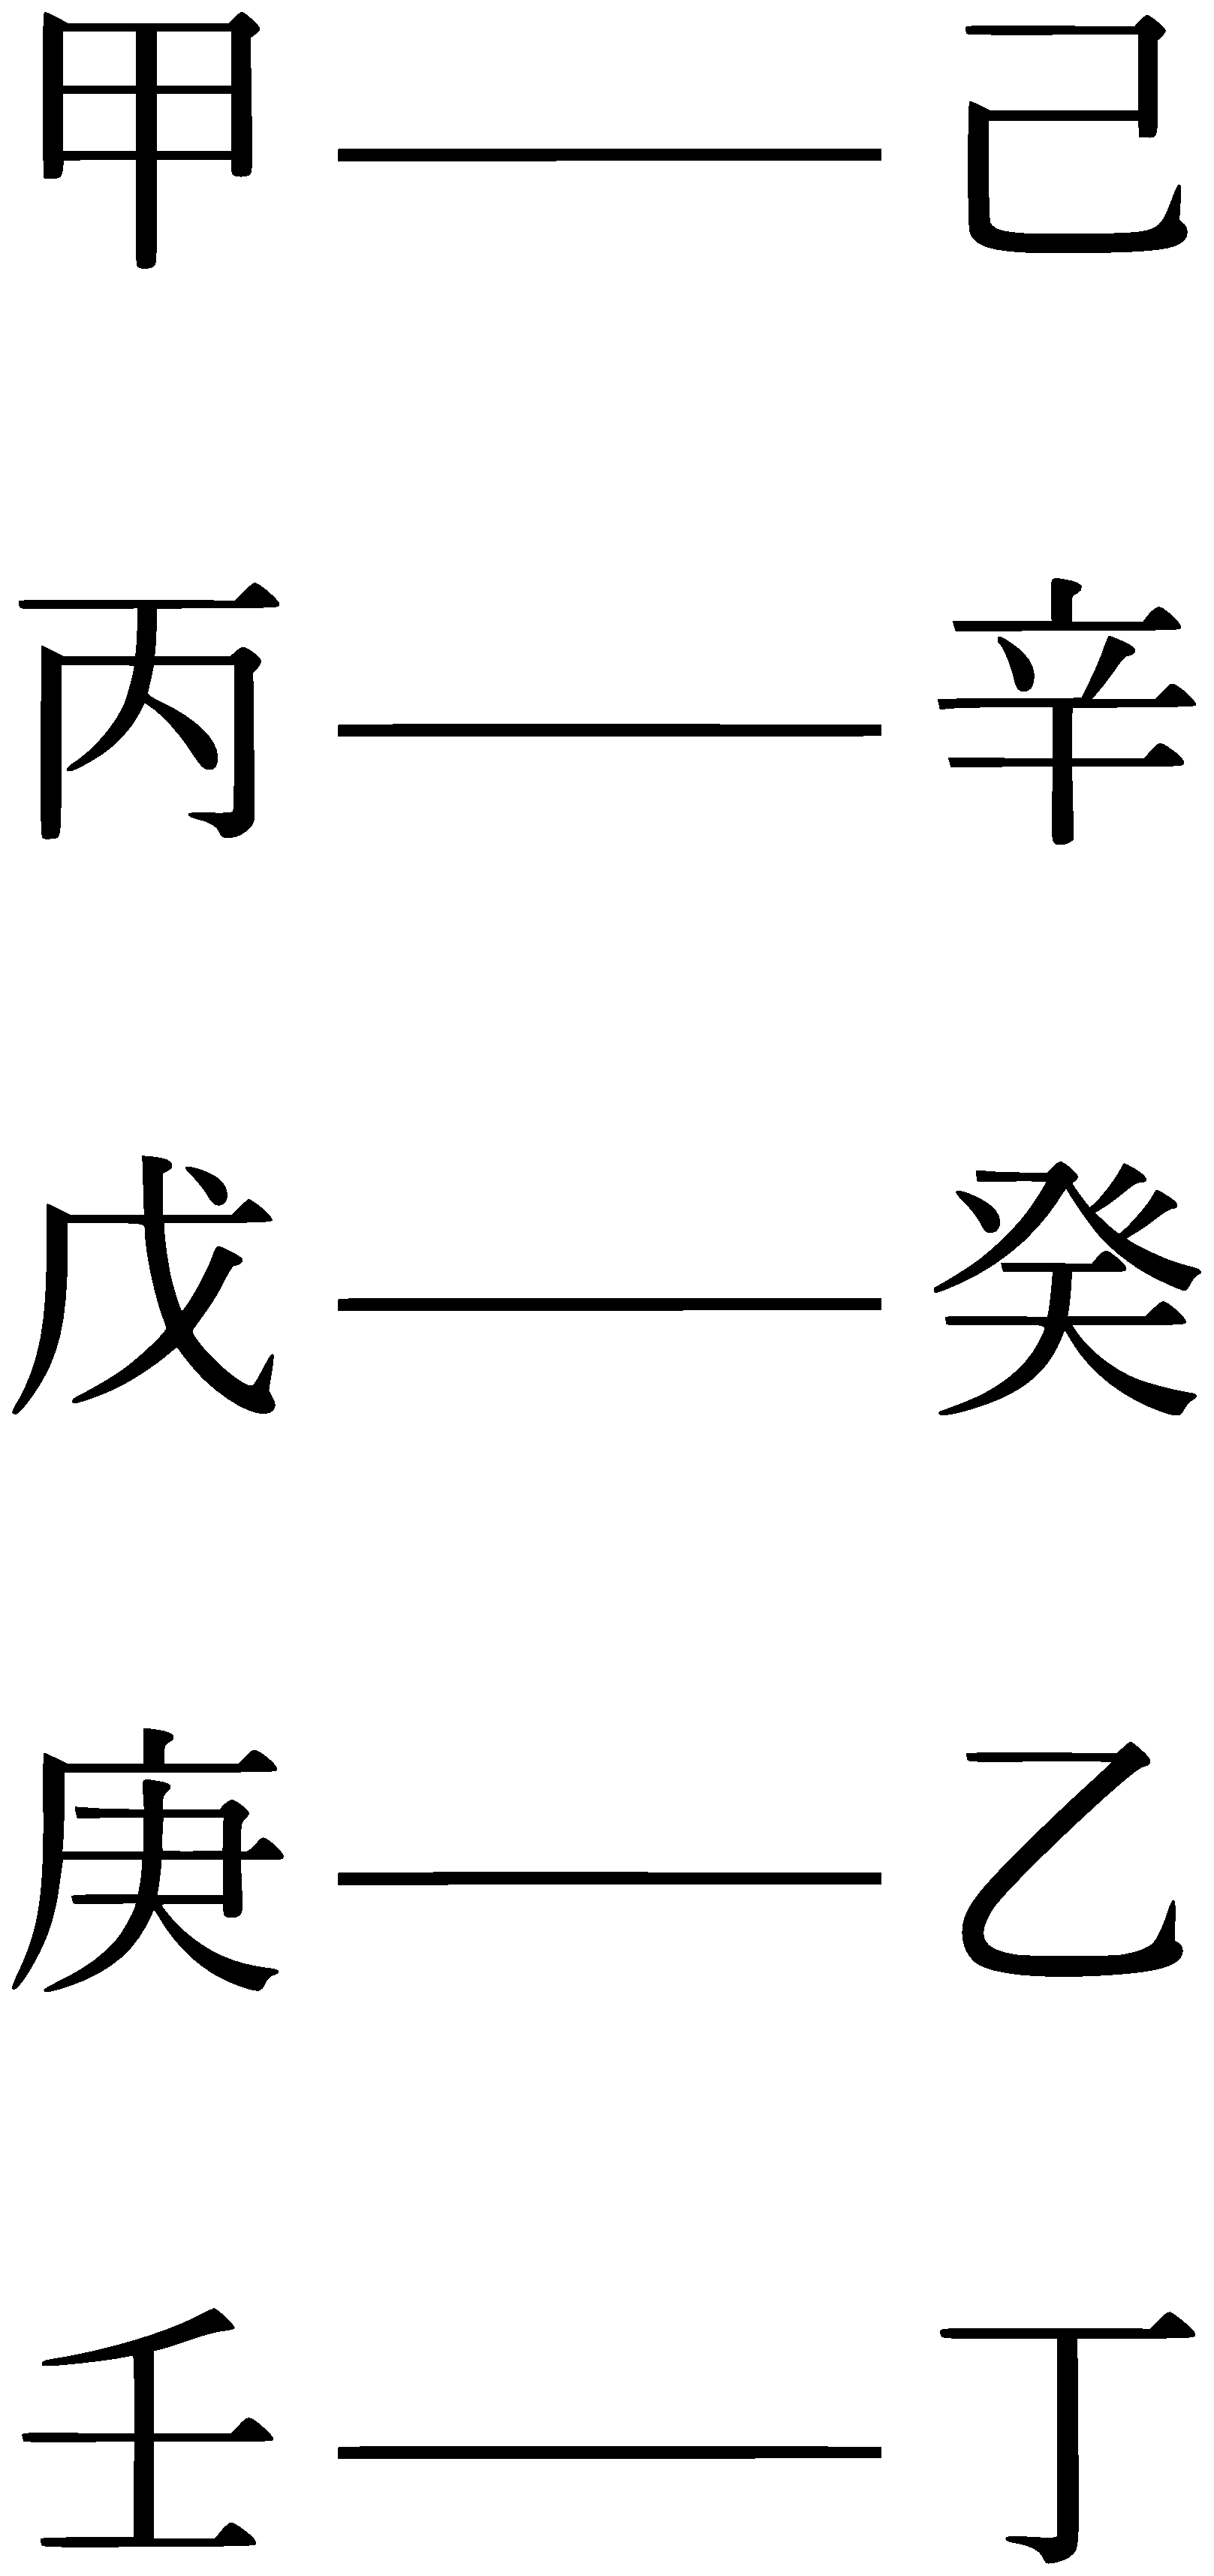
\includegraphics[width=20mm,angle=90]{figs/table7-1.eps}
\end{figure}

次の命式を例にして、干合による変化を説明します。

\begin{figure}[h]
  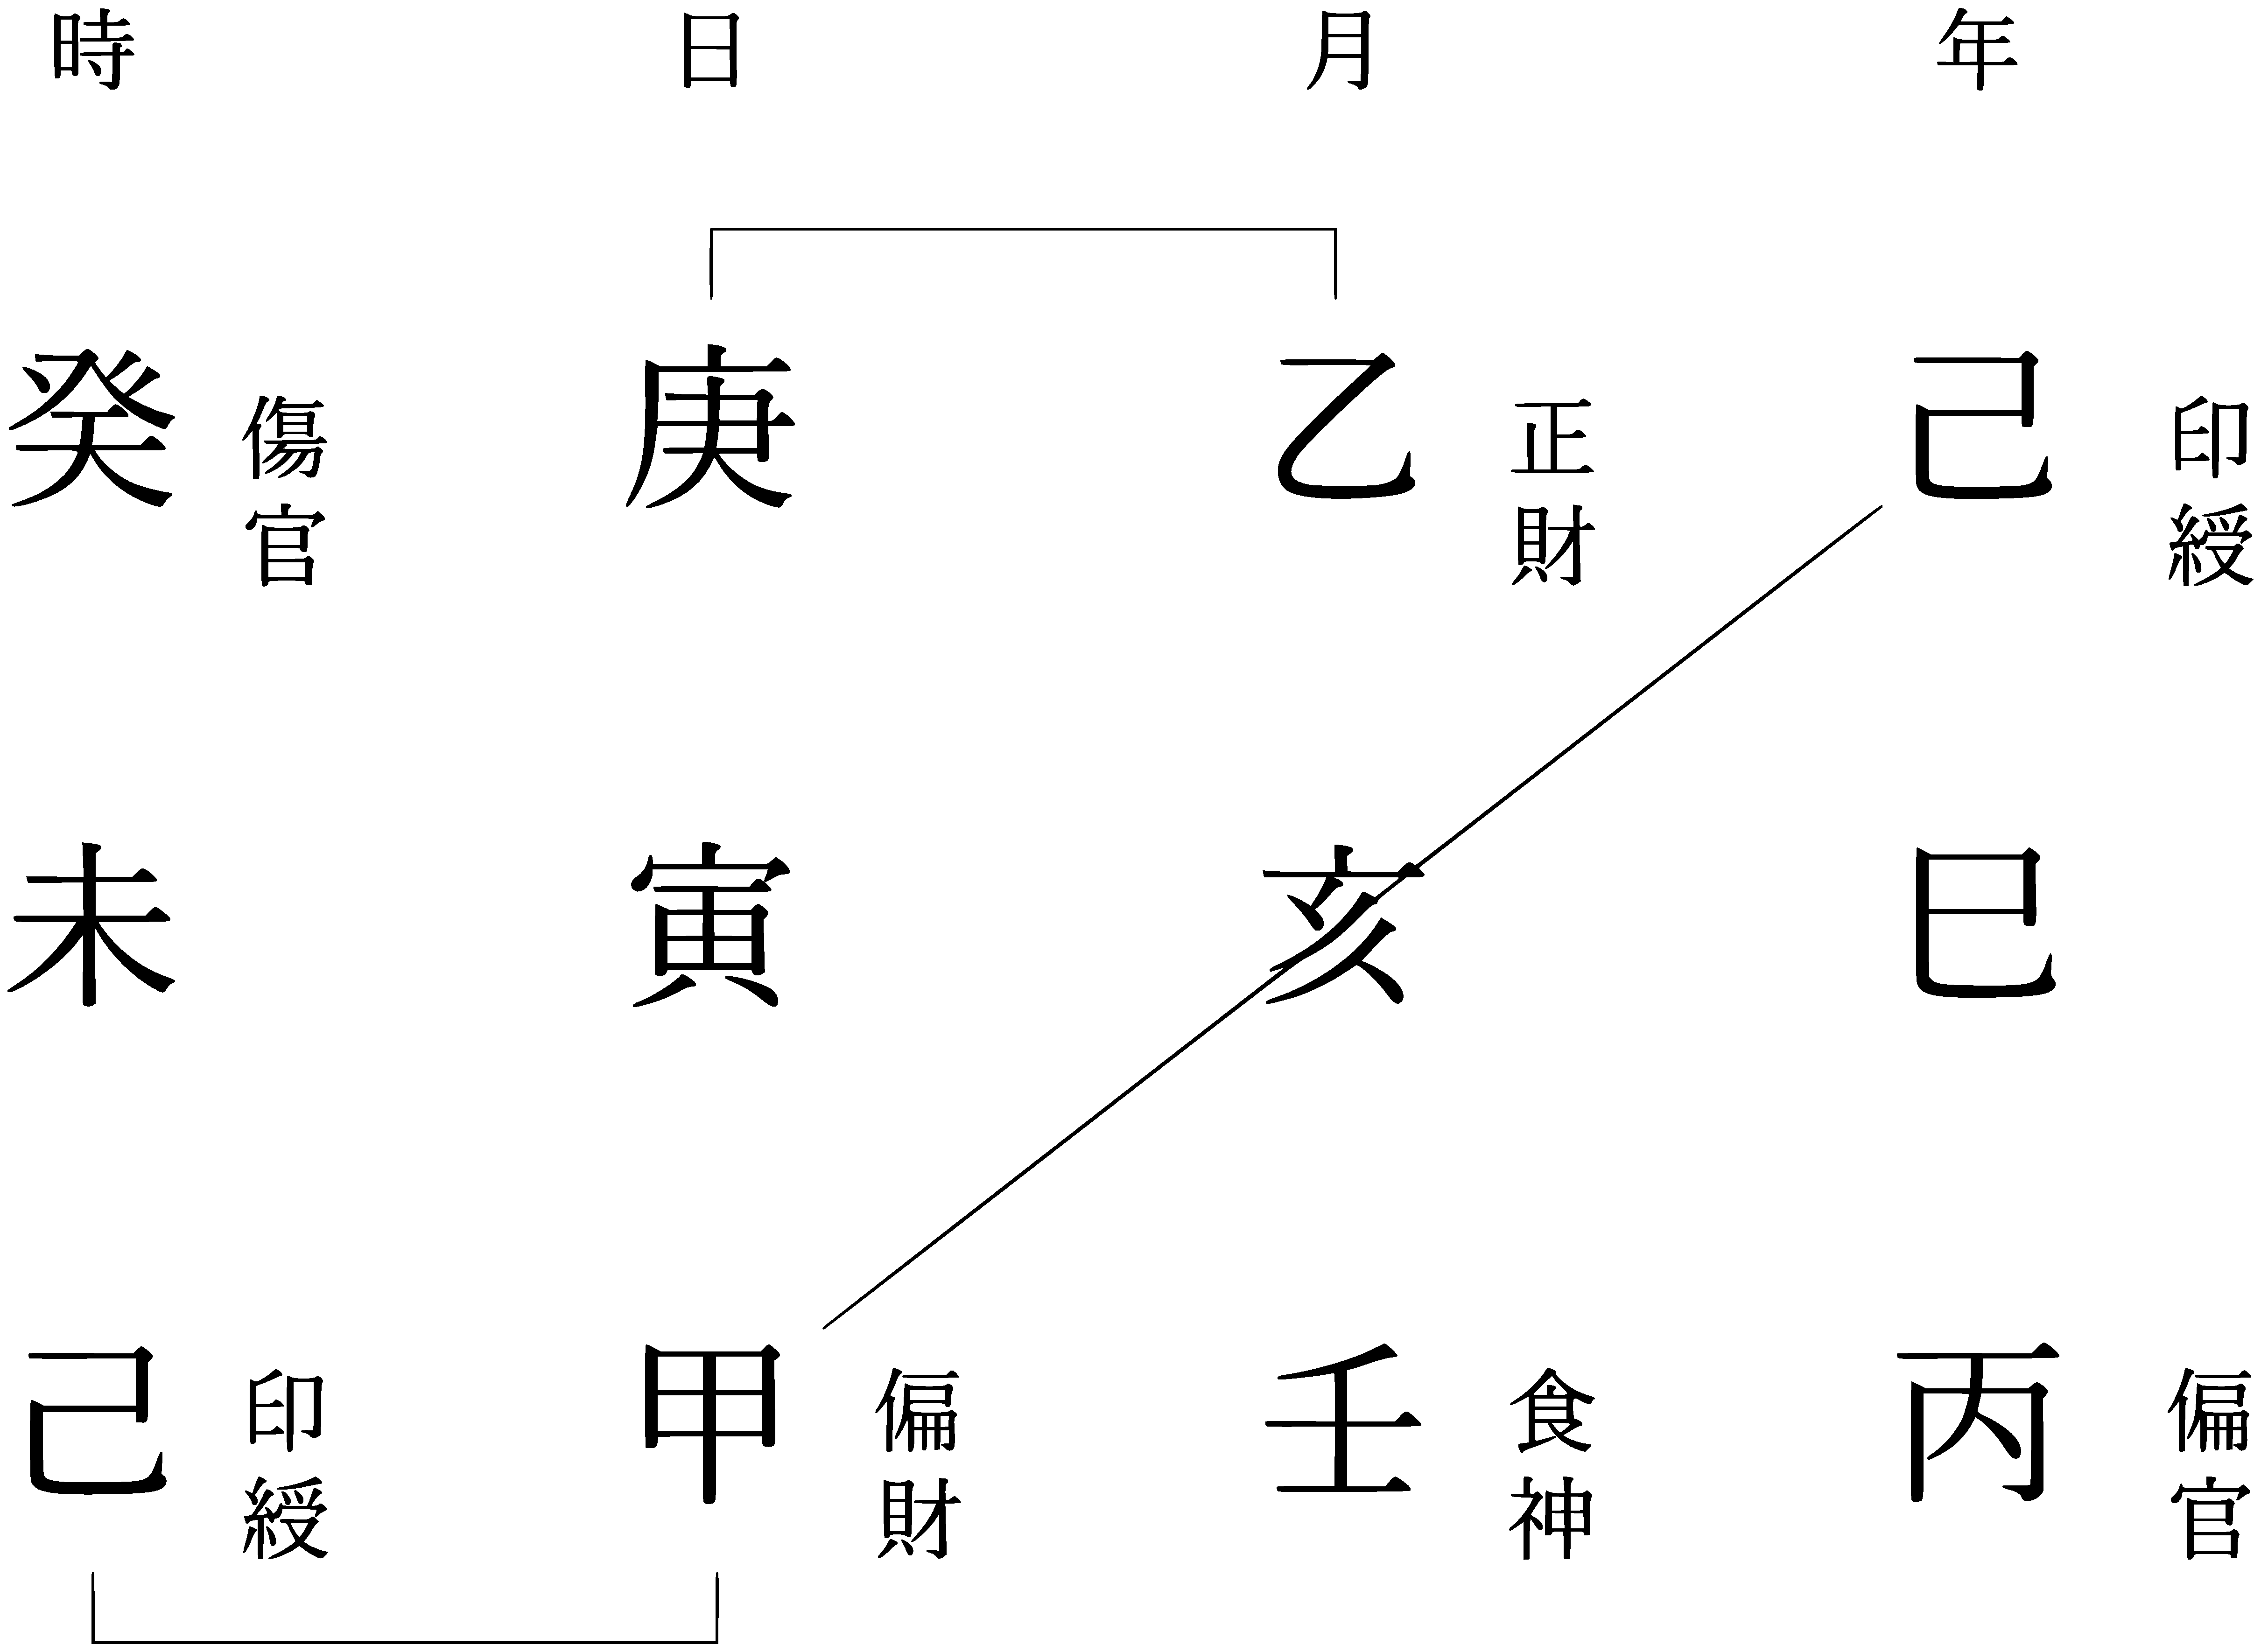
\includegraphics[width=60mm,angle=90]{figs/figure7-1.eps}
\end{figure}

この命式では、日干の庚と月柱天干の乙とが干合しています。このように、日干と他の干が干合したとき、他の干の通変が良い通変である場合は、その吉の作用が倍加し、悪い通変である場合は、その凶の作用が減じられます。つまり、日干に干合があるのは、基本的に喜ばしいのです。この命式では、良い通変である乙正財による吉の作用が大きくなります。

また、この命式では、日柱蔵干の甲と時柱蔵干の己とが干合しています。このように、日干以外の干同士が干合したとき、良い通変であっても悪い通変であっても、それらの作用が減じられます。この命式では、良い通変である甲偏財も己印綬も、それらの吉の作用が減じられます。

ところで、この命式では、日柱蔵干の甲は年柱天干の己とも干合しています。このように干合が重複する(一対多になる)ことを\ruby{妬合}{とごう}といい、この状態を嫌います。

\subsection{支の変化}

\subsubsection*{支合}
干と同様に、支にも互いに「仲良し」なペアがあります。命式中にこのペアが揃った場合、それらの支が\ruby{支合}{しごう}して変化が現れます。

次の表は、支合する支のペアを列挙したものです。

\begin{figure}[h]
 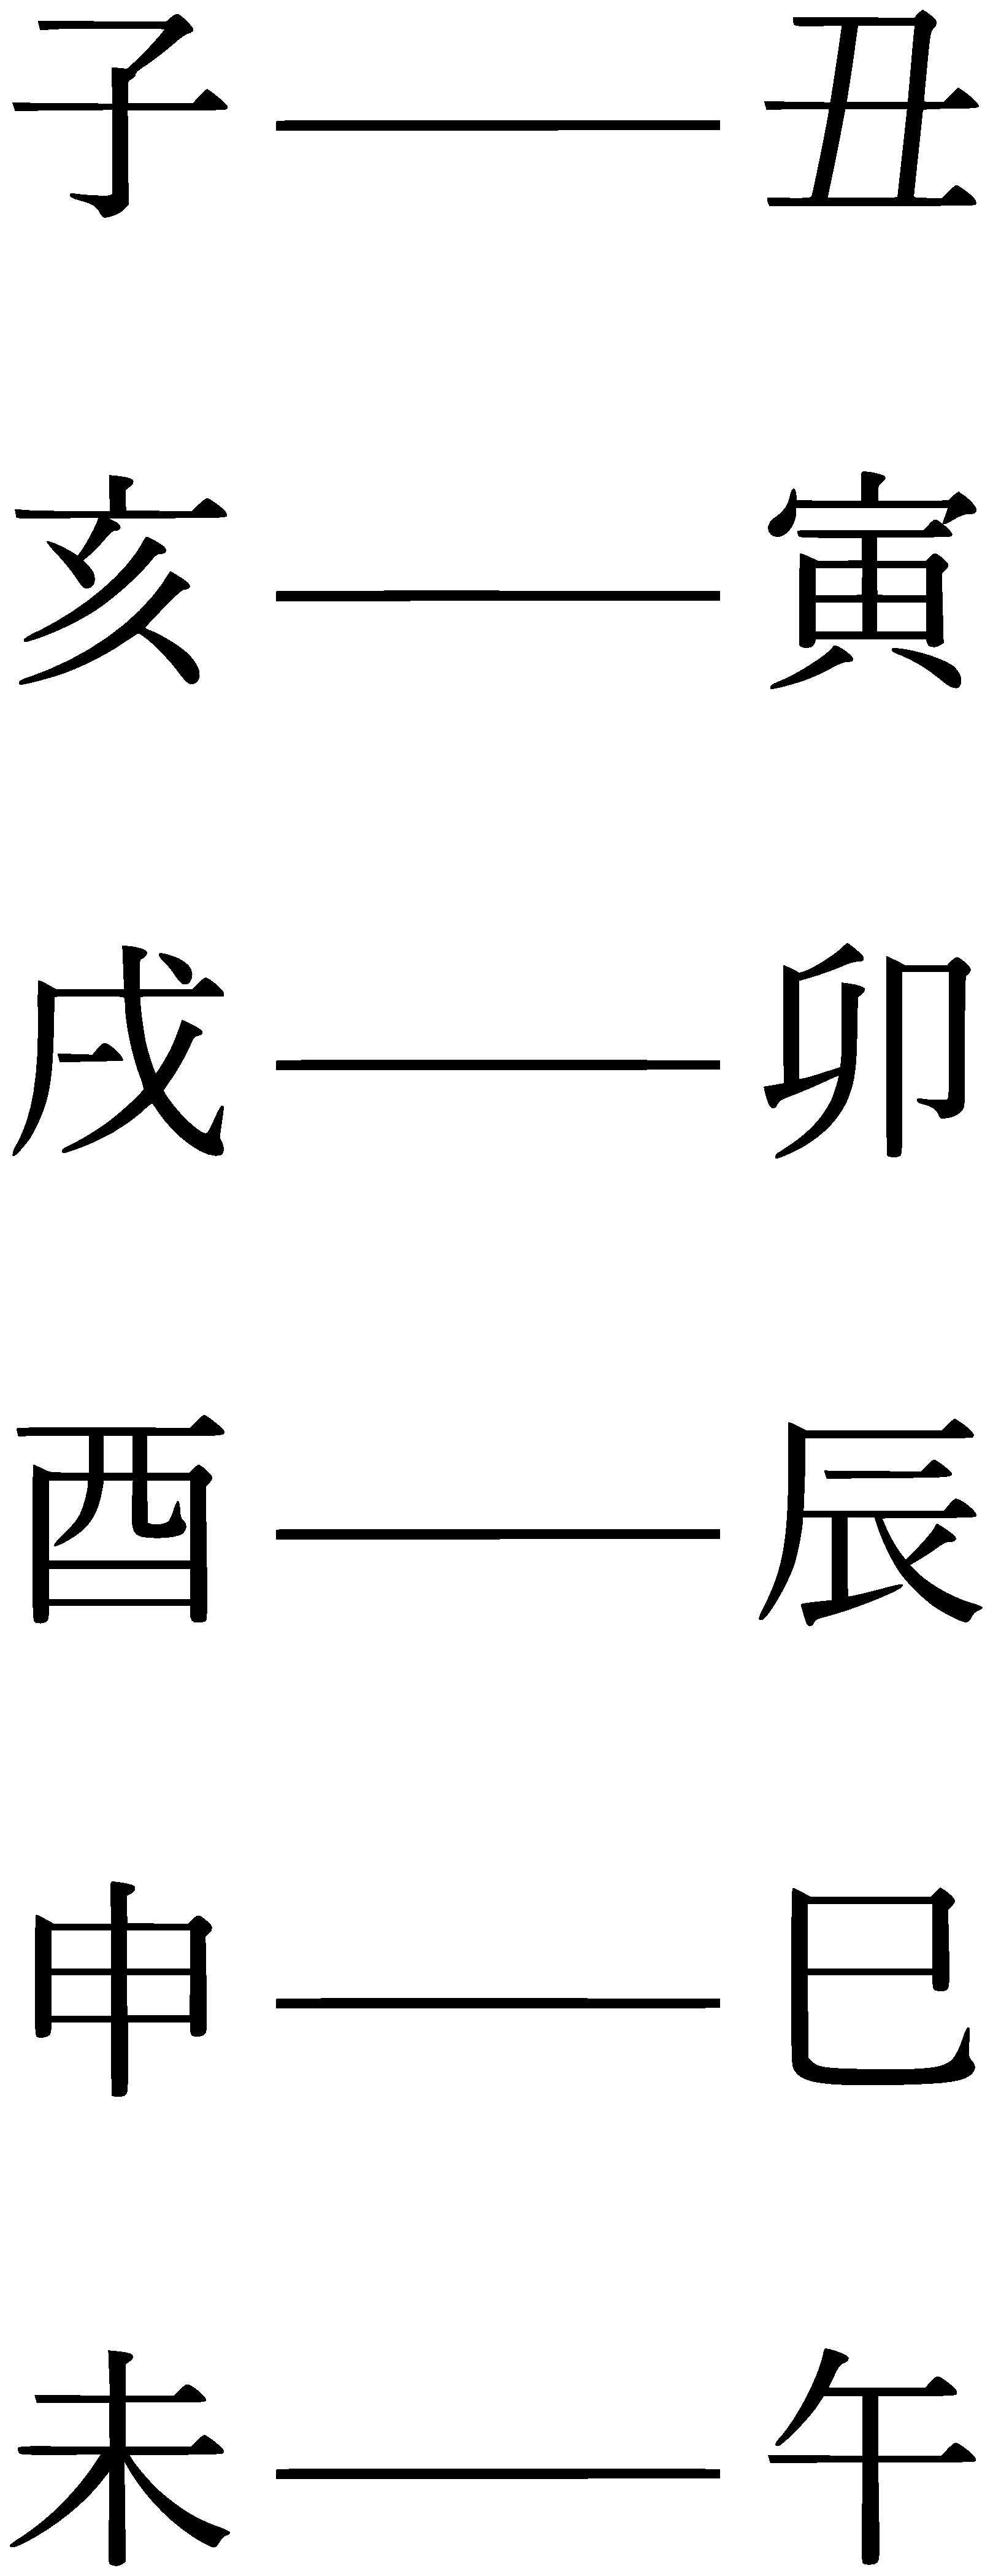
\includegraphics[width=20mm,angle=90]{figs/table7-2.eps}
\end{figure}

支合のある柱同士は結束が強くなるため、それらの柱にある吉の作用は倍加し、凶の作用は減じられます。つまり、支合があるのは喜ばしいのです。

先の命式を再掲し、支合による変化を説明します。

\begin{figure}[h]
  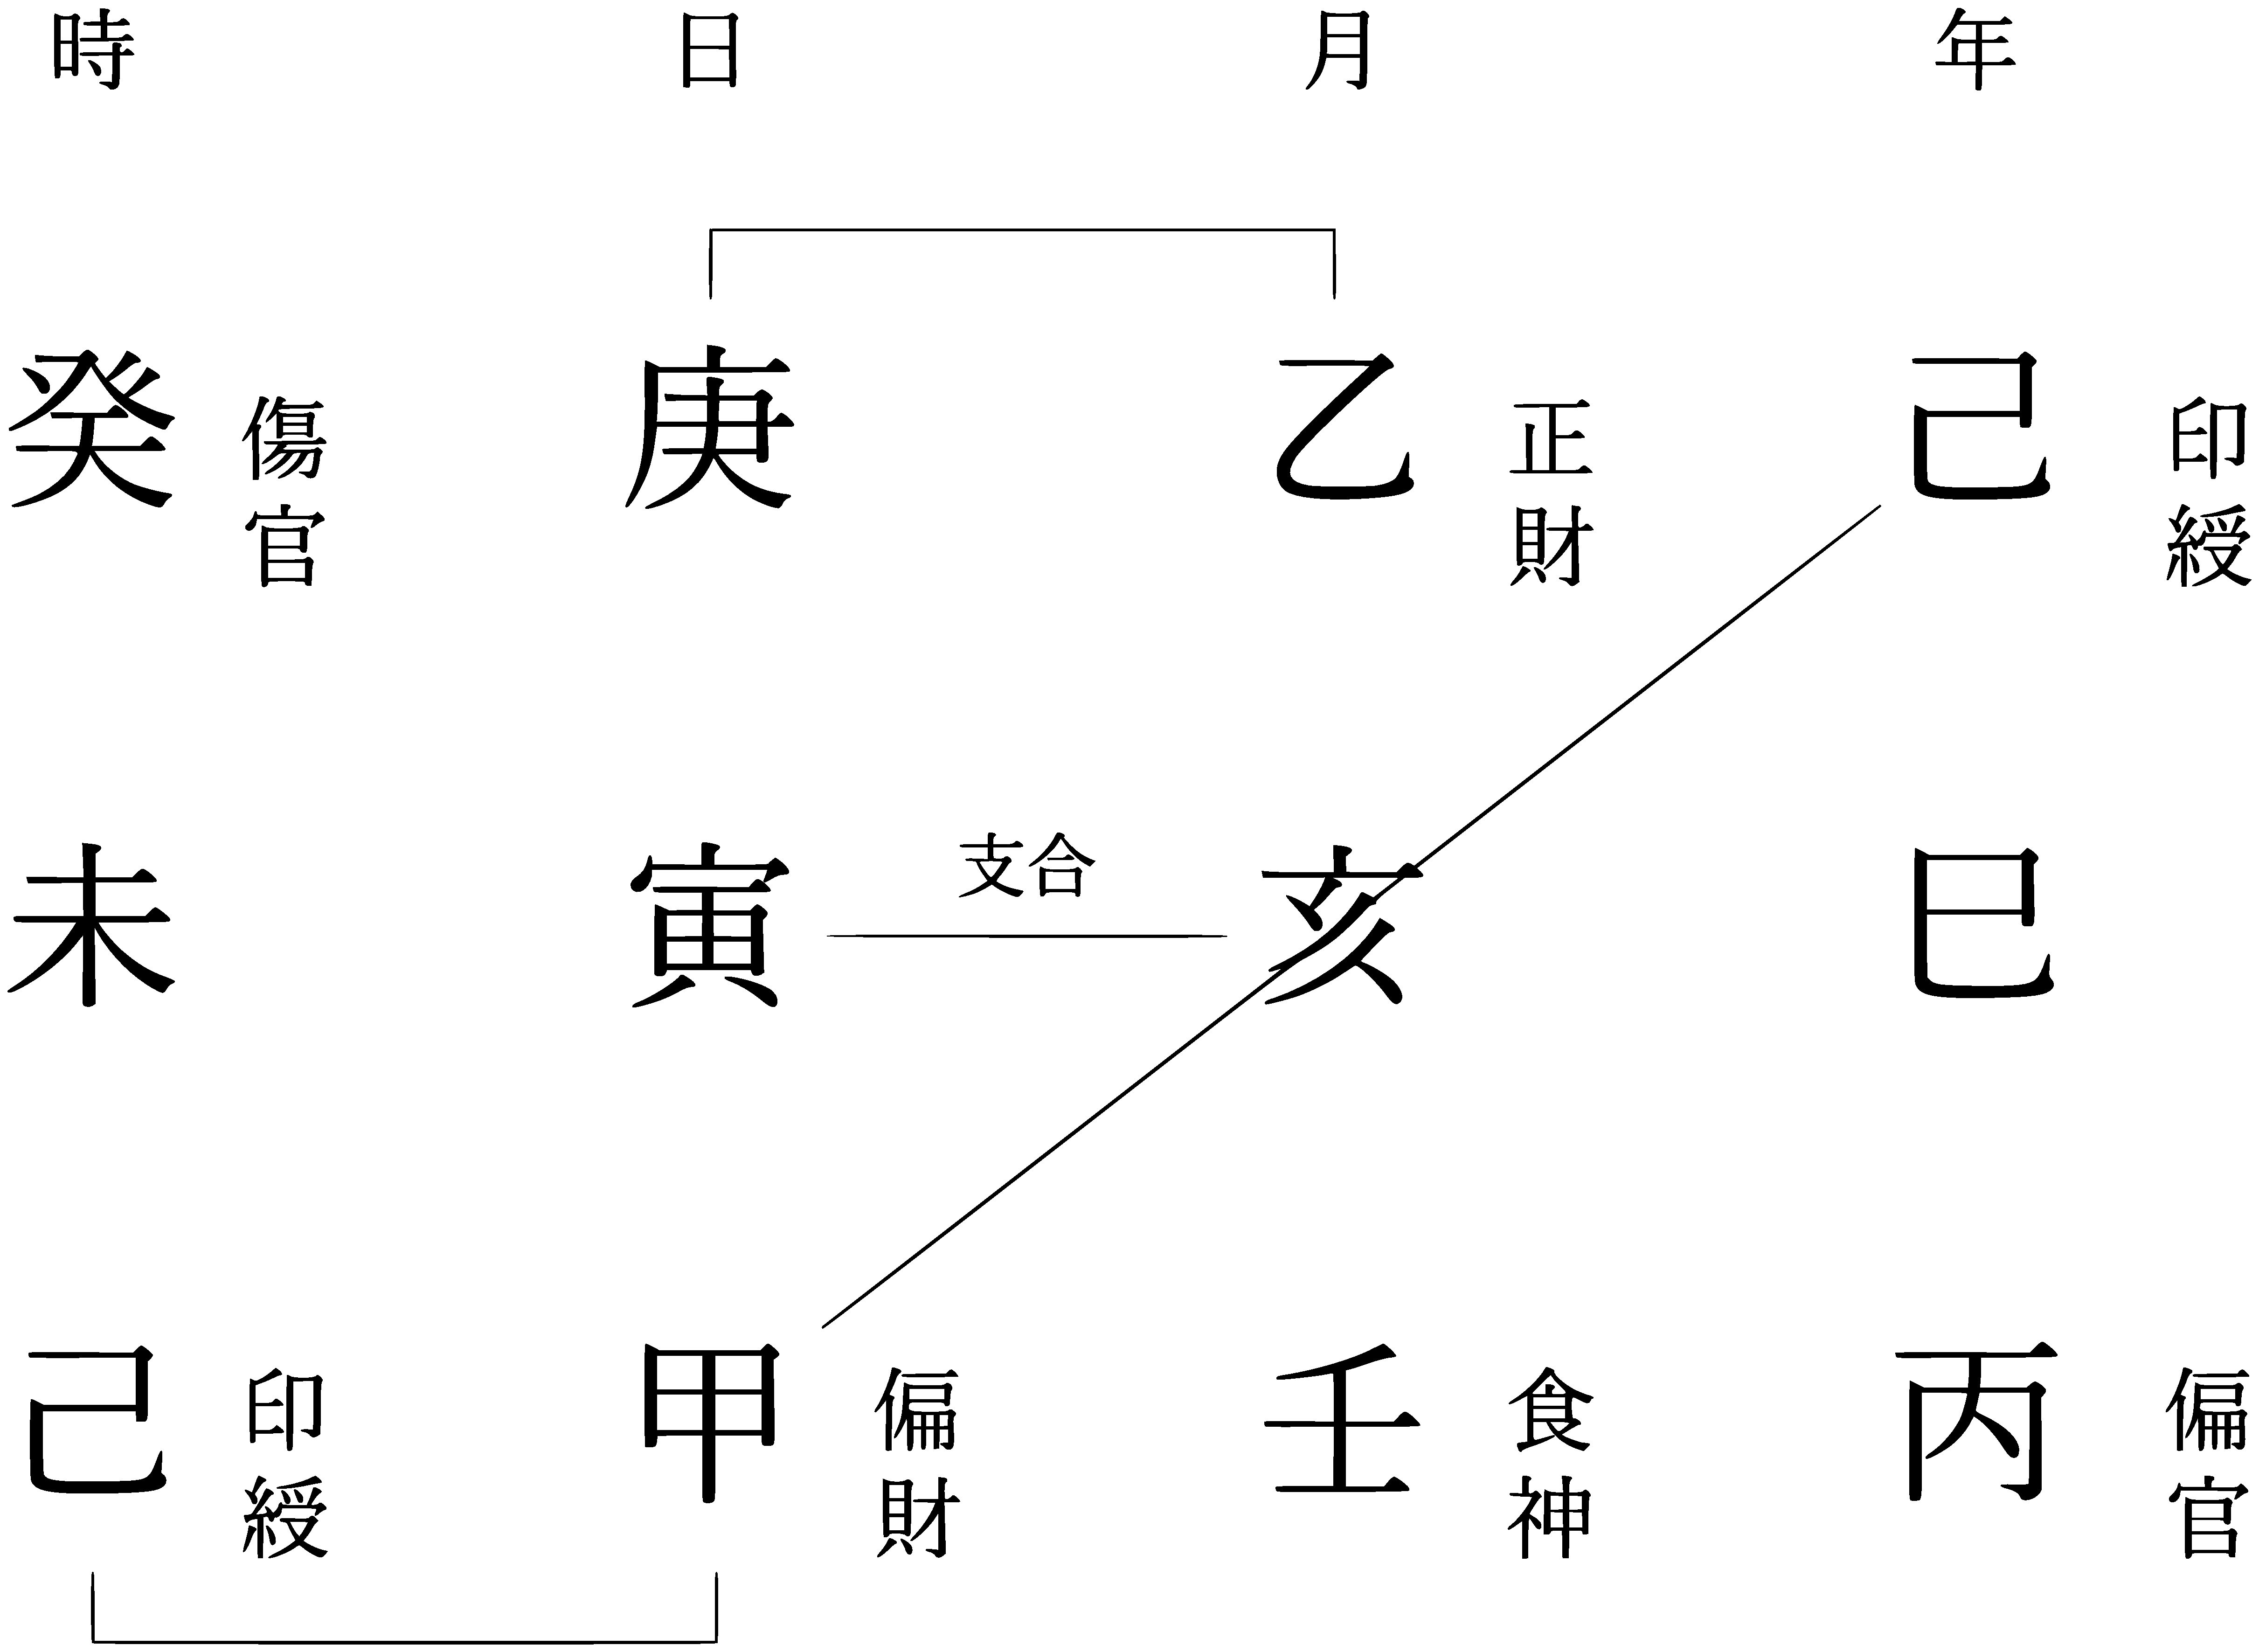
\includegraphics[width=60mm,angle=90]{figs/figure7-2.eps}
\end{figure}

この命式では、日支の寅と月支の亥が支合しています。そのため、まず日干の強さが増します。同時に、甲偏財、乙正財、壬食神による吉の作用も増します。

\subsubsection*{方合}
同じ季節を表す三つの支が揃うと\ruby{方合}{ほうごう}となります。

【表7−3】

\begin{figure}[h]
  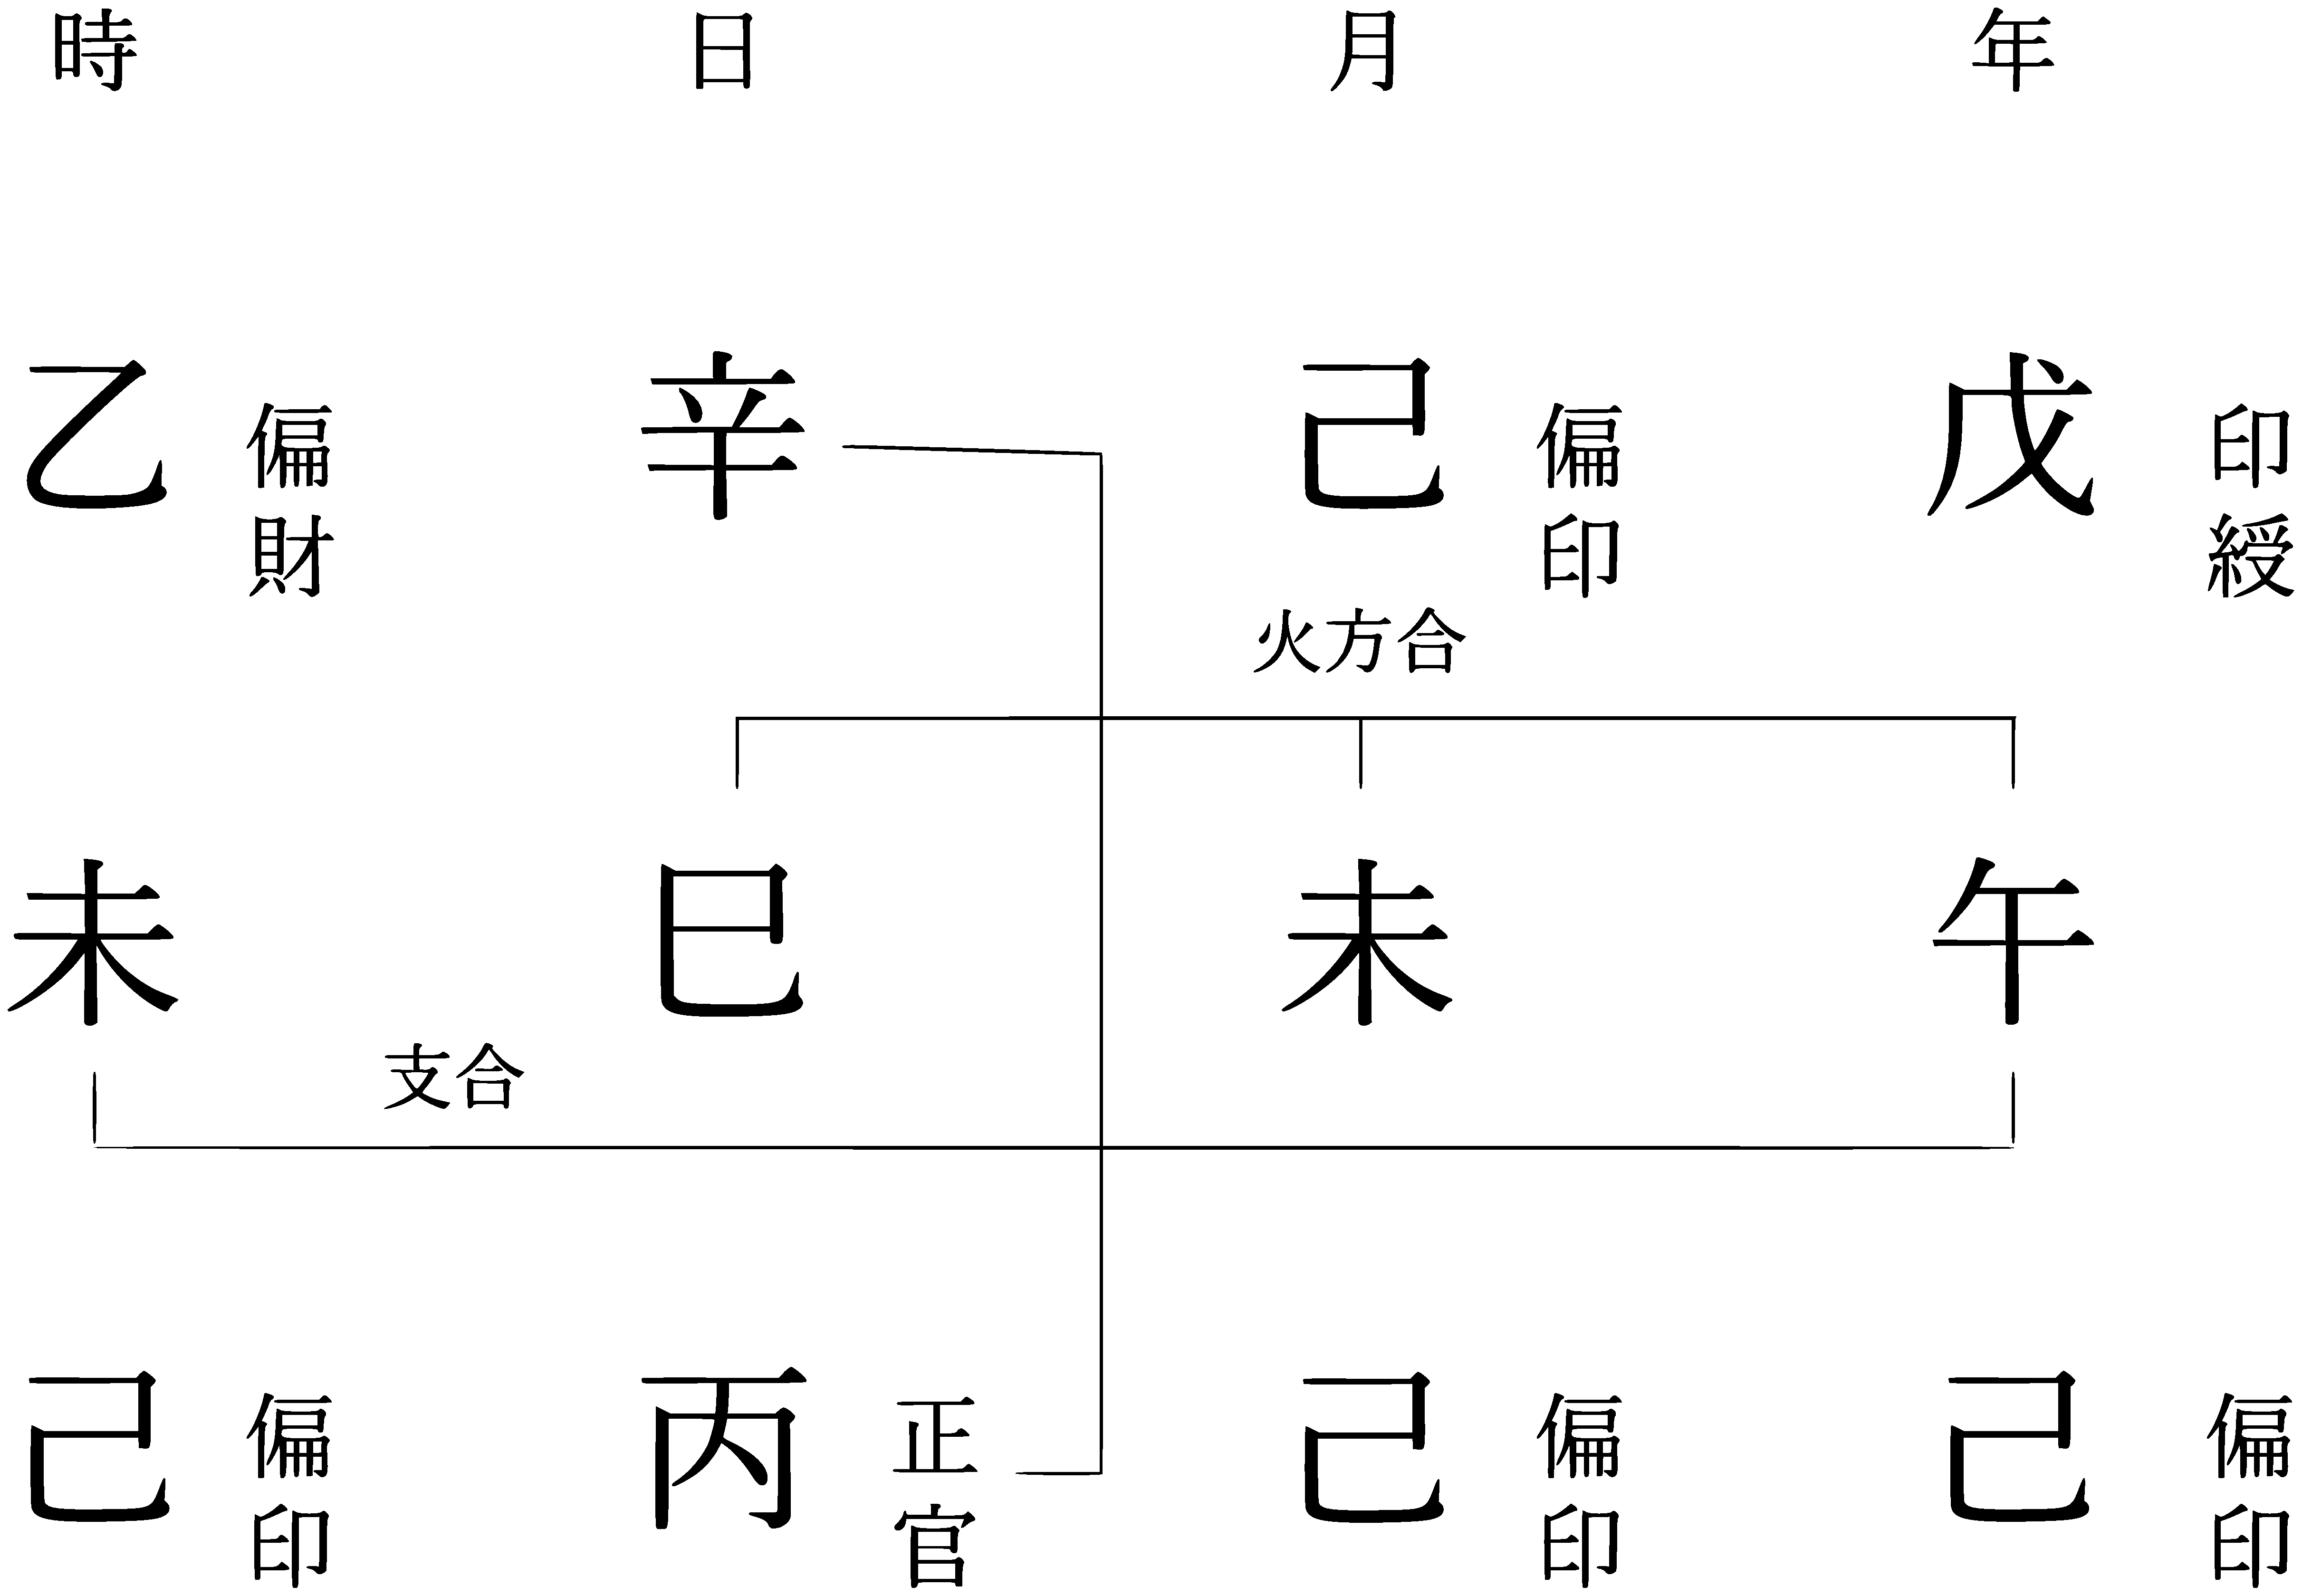
\includegraphics[width=60mm,angle=90]{figs/figure7-3.eps}
\end{figure}

なお、この命式では、日干の辛と日柱蔵干の丙とが干合しています。
このように、天干と蔵干が干合することを「\ruby{自化干合}{じかかんごう}」といい、大変良い作用をもたらします。

\subsubsection*{三合・半会}
\ruby{三合}{さんごう}とは、子・卯・午・酉を中心とする特別な三つの支の組み合わせです。\footnote{子・卯・午・酉は、各季節の真ん中に位置する支であり、これらを「\ruby{四聖}{しせい}」と呼びます。}

【表7−4】

三合の支が命式中に揃っていれば、その五行の気勢は大変強いと考えます。これを\ruby{三合会局}{さんごうかいきょく}といい、\ruby{合}{ごう}(\ruby{支合}{しごう}・\ruby{方合}{ほうごう}・\ruby{三合}{さんごう})の中で最も重要です。

【図7−4】

\subsubsection*{七冲}
支合が互いに「仲良し」なペアである一方で、\ruby{七冲}{ひつちゅう}は互いに「仲の悪い」支のペアです。

次の表は、\ruby{冲}{ちゅう}する支のペアを列挙したものです。\footnote{\ruby{七冲}{ひつちゅう}は、単に「\ruby{冲}{ちゅう}」と略す場合があります。}

【表7−5】

\ruby{七冲}{ひつちゅう}には向きがあることに注意しましょう。

命式中に冲があれば、

次の命式を例にして、\ruby{七冲}{ひつちゅう}による影響を説明します。

【図7−5】


解冲


\subsubsection*{刑}


\subsubsection*{害}


\subsubsection*{空亡}


解空


\subsection{大運・年運との組み合わせ}



\clearpage




\section{看命の基本}

【図9−1】

\begin{enumerate}
\item 五行\\
水が欠けており、五行周流していません。
\item 日干\\
  日干辛は月令を得ています。十二運はビ・建・ゼ・スとあまり旺じていませんが、通変には比肩二つ、印綬一つ、偏印二つがあり、強力に日干を比助しています。また、月柱が金で\ruby{透干}{とうかん}しており、さらに日干を強めます。日干は中強を超えて大強に近いと判断します。
  
\item 調候\\

\item 格\\
月支蔵干は比肩のため、これを用神とすることはできません。そのため、時柱天干にあって良い通変である偏財を用神とします。
この命式は偏財格です。

用神乙は月令を得ていません。十二運は長・ゼ・建・養と旺じていますが、通変に偏財(日支蔵干)しかありません。ただし、命式中に木半会があり、これが用神乙を強めています。かろうじて小強程度と判断します。
\item 成格・破格\\
日干が極めて強いのに対して、用神が頼りなく、典型的な「ワンマン会社」になっています。日干と格との均衡は大きく崩れているため、破格と認定します。\\
\end{enumerate}


破格となったこの命式が成格に近づくためには、日干が衰弱し、用神が旺じることにより、日干対格のバランスが保たれる必要があります。
\begin{description}
\item[(ア)] 日干が衰弱する\\
まず、日干辛が月令を得なくなる時期(春・夏・冬)を喜びます。次に、日干辛(金)の力を洩らす食神・傷官(水)が大運・年運に巡ることを喜びます。さらに、日干を剋す火が方合・三合・半会によって強まる時期を喜びます。
\item[(イ)] 用神が旺じる\\
まず、用神乙が月令を得る時期(春・冬)を喜びます。次に、用神乙(木)に力を与える食神・傷官(水)、正財・偏財(木)が大運・年運に巡ることを喜びます。さらに、用神の比和である木が方合・三合・半会によって強まる時期を喜びます。
\end{description}

逆に、破格がさらに破格に近づいてしまう条件は、日干がますます旺じ、用神が衰弱することです。
\begin{description}
\item[(ウ)] 日干がますます旺じる\\
まず、日干が月令を得る時期(秋・土用)を嫌います。次に、日干辛を比助する比肩・劫財・印綬・偏印が大運・年運に巡ることを嫌います。さらに、日干の比和である金が方合・三合・半会によって強まる時期を嫌います。
\item[(エ)] 用神が衰弱する\\
まず、用神が月令を得なくなる時期(夏・秋・土用)を嫌います。次に、用神乙を剋す比肩・劫財が大運・年運に巡ることを嫌います。
\end{description}

これら(ア)〜(エ)を頭に入れた上で大運を読み、成格に近づく時期を「運気が良い」とし、逆に破格に近づく時期を「運気が悪い」とします。

\begin{enumerate}
\setcounter{enumi}{5}
\item 大運\\
○壬戌/傷官(4〜\rensuji{13}歳)
  
 季節は秋のため、日干辛は月令を得て旺じています。ここだけを見ると、強い日干がさらに強くなってよくありません。しかし、年支午と大運支戌の火半会によって日干が抑えられるとともに、大運通変の壬傷官が欠けた水を補うことによって五行周流し、日干の力を洩らします。これらを総合すれば、運気としては悪くないと言えるでしょう。\\

◎癸亥/食神(\rensuji{14}〜\rensuji{23}歳)

 季節は冬に入ります。日干辛は月令を得ない一方で、用神乙は月令を得ます。また、日支卯・時支未・大運支亥で三合木局を構成し、強力に用神乙を強めます。さらに、大運通変の癸食神が欠けた水を補うことによって日干の力を洩らします。これにより、日干に大きく傾いていた命式がバランスを取り戻し、立派な成格に変貌します。この時期の運気は最高潮で、素晴らしい青春時代を送れると期待できます。\\

○甲子/正財(\rensuji{24}〜\rensuji{33}歳)

 大運の干支は「水生木」の関係にある(子から甲が生じられる)ため、この時期は木に勢いがあります。そのため、月令を得た用神乙はますます旺じます。日干辛との均衡はまずまずと考えられ、運気としては悪くないでしょう。\\

△乙丑/偏財(\rensuji{34}〜\rensuji{43}歳)

 用神乙は引き続き月令を得ますが、同時に日干辛も月令を得ます。おまけに、月支酉と大運支丑の金半会によって日干が強められます。日干対格のバランスは日干側に倒れ、破格に近づきます。注意が必要な\rensuji{10}年間となるでしょう。

 なお、この時期の年運に巳年が巡ると、月支酉・大運支丑・年運支巳の三合金局を構成します。日干がますます強くなり、さらにバランスが崩れるため、特に注意が必要な1年になります。\\

◎丙寅/正官(\rensuji{44}〜\rensuji{53}歳)

 季節は春に入ります。日干辛は月令を得ておらず、用神乙は月令を得ています。大運の干支は「木生火」の関係にある(寅から丙が生じられる)ため、この時期は火に勢いがあります。大運通変の丙正官が日干辛を剋すとともに、年支午と大運支寅の強力な火半会によって日干が抑えられます。再び立派な成格に変貌し、運気は上々です。輝かしい中年期として活躍が期待されるでしょう。

 なお、この時期の年運に辰年が巡ると、大運支寅・日支卯・年運支辰の木方合を構成します。また、戌年が巡ると、年支午・大運支寅・年運支戌の三合火局を構成します。これらの年では特に運気が上昇し、ますますの発展が望めるでしょう。\\

○丁卯/偏官(\rensuji{54}〜\rensuji{63}歳)

 引き続き日干辛は月令を得ておらず、用神乙は月令を得ています。時支未と大運支卯で木半会が新たに生じ、これが用神を強めます。日干との均衡はまずまずと考えられ、運気としては悪くないでしょう。\\

△戊辰/印綬(\rensuji{64}〜\rensuji{73}歳)

 用神乙は引き続き月令を得ますが、同時に日干辛も月令を得ます。また、大運通変の戊印綬が日干を強めるため、日干対格のバランスは日干側に倒れます。注意が必要な\rensuji{10}年間となるでしょう。\\

△己巳/偏印(\rensuji{74}〜\rensuji{83}歳)

 季節は夏に入ります。日干・用神ともに月令を得ていません。\\


なお、この時期の年運に丑年が巡ると、月支酉・大運支巳・年運支丑の三合金局を構成します。日干がますます強くなり、さらにバランスが崩れるため、特に注意が必要な1年になります。


×庚午/劫財(\rensuji{84}〜\rensuji{93}歳)

×辛未/比肩(\rensuji{94}〜\rensuji{103}歳)


\item 性格\\
   まず、なんといっても日干が強いので、非常に「我が強い」ことが特徴です。強気で我が道をゆくことに生きがいを感じ、多少のリスクがあっても新しいことにどんどんチャレンジします。積極的に手を広げるため、その人生は浮き沈みの激しい面を持ちます。自分の力を過信しやすく、周囲から孤立する場合があるので、状況に応じて我を抑える意識が必要になるでしょう。
  
   また、月支蔵干通変である「比肩」の性質が強く表に現れます。自分の力で何かを成し遂げるプロセスを経て、達成感を得ることに生き甲斐を感じるタイプです。ピュアで裏表がなく、嘘をついたり人を裏切ったりしないため、周りから信頼を得られるでしょう。
  
   不器用なほど自分のペースとこだわりを守ろうとするため、周囲を困惑させることがあるかもしれません。とにかく強く我を通そうとするため、身近な人とトラブルになる場合があるのが心配です。行動力があり、目標に向かって努力できるので、少し我を抑えれば活躍の幅は徐々に広がっていきます。
  
   自分で本当に納得しなければ、絶対に人の言うことを受け入れません。逆に、自分で納得して一度決めたことは、トコトン貫く意志の強さがあります。一方で、一本気なパワーをまっすぐに生かすためには、意地を張らず、頑固になりすぎず、たまには他人のアドバイスを素直に聞くことが重要と言えるでしょう。
  
   次に、日支蔵干通変である「偏財」の性質が現れます。一つのことをじっくり掘り下げるのは苦手です。次から次に色々なアイデアが浮かぶので、忘れないうちに実際に試してみたい衝動に駆られるからです。そのため、どうしても多動的になり、いつもバタバタしている落ち着きのない人だと思われているかもしれません。
  
   選択を迫られる場面では、損か得かで判断する傾向があります。目先の利益に左右されず、感情にも流されないのは、優れた大人の判断です。行動的で嗅覚に恵まれたことを誇りに思い、有意義に生かしましょう。
  
 コミュニケーション能力が高く、ユーモアのセンスがあり、何事にもマメです。ただし、誰かと会話をするときは、自分の話を抑えて相手を立て、聞き役にまわることを意識することが重要です。

\end{enumerate}


\end{document}
